\documentclass[twoside]{book}

% Packages required by doxygen
\usepackage{fixltx2e}
\usepackage{calc}
\usepackage{doxygen}
\usepackage[export]{adjustbox} % also loads graphicx
\usepackage{graphicx}
\usepackage[utf8]{inputenc}
\usepackage{makeidx}
\usepackage{multicol}
\usepackage{multirow}
\PassOptionsToPackage{warn}{textcomp}
\usepackage{textcomp}
\usepackage[nointegrals]{wasysym}
\usepackage[table]{xcolor}

% Font selection
\usepackage[T1]{fontenc}
\usepackage[scaled=.90]{helvet}
\usepackage{courier}
\usepackage{amssymb}
\usepackage{sectsty}
\renewcommand{\familydefault}{\sfdefault}
\allsectionsfont{%
  \fontseries{bc}\selectfont%
  \color{darkgray}%
}
\renewcommand{\DoxyLabelFont}{%
  \fontseries{bc}\selectfont%
  \color{darkgray}%
}
\newcommand{\+}{\discretionary{\mbox{\scriptsize$\hookleftarrow$}}{}{}}

% Page & text layout
\usepackage{geometry}
\geometry{%
  a4paper,%
  top=2.5cm,%
  bottom=2.5cm,%
  left=2.5cm,%
  right=2.5cm%
}
\tolerance=750
\hfuzz=15pt
\hbadness=750
\setlength{\emergencystretch}{15pt}
\setlength{\parindent}{0cm}
\setlength{\parskip}{3ex plus 2ex minus 2ex}
\makeatletter
\renewcommand{\paragraph}{%
  \@startsection{paragraph}{4}{0ex}{-1.0ex}{1.0ex}{%
    \normalfont\normalsize\bfseries\SS@parafont%
  }%
}
\renewcommand{\subparagraph}{%
  \@startsection{subparagraph}{5}{0ex}{-1.0ex}{1.0ex}{%
    \normalfont\normalsize\bfseries\SS@subparafont%
  }%
}
\makeatother

% Headers & footers
\usepackage{fancyhdr}
\pagestyle{fancyplain}
\fancyhead[LE]{\fancyplain{}{\bfseries\thepage}}
\fancyhead[CE]{\fancyplain{}{}}
\fancyhead[RE]{\fancyplain{}{\bfseries\leftmark}}
\fancyhead[LO]{\fancyplain{}{\bfseries\rightmark}}
\fancyhead[CO]{\fancyplain{}{}}
\fancyhead[RO]{\fancyplain{}{\bfseries\thepage}}
\fancyfoot[LE]{\fancyplain{}{}}
\fancyfoot[CE]{\fancyplain{}{}}
\fancyfoot[RE]{\fancyplain{}{\bfseries\scriptsize Generated by Doxygen }}
\fancyfoot[LO]{\fancyplain{}{\bfseries\scriptsize Generated by Doxygen }}
\fancyfoot[CO]{\fancyplain{}{}}
\fancyfoot[RO]{\fancyplain{}{}}
\renewcommand{\footrulewidth}{0.4pt}
\renewcommand{\chaptermark}[1]{%
  \markboth{#1}{}%
}
\renewcommand{\sectionmark}[1]{%
  \markright{\thesection\ #1}%
}

% Indices & bibliography
\usepackage{natbib}
\usepackage[titles]{tocloft}
\setcounter{tocdepth}{3}
\setcounter{secnumdepth}{5}
\makeindex

% Hyperlinks (required, but should be loaded last)
\usepackage{ifpdf}
\ifpdf
  \usepackage[pdftex,pagebackref=true]{hyperref}
\else
  \usepackage[ps2pdf,pagebackref=true]{hyperref}
\fi
\hypersetup{%
  colorlinks=true,%
  linkcolor=blue,%
  citecolor=blue,%
  unicode%
}

% Custom commands
\newcommand{\clearemptydoublepage}{%
  \newpage{\pagestyle{empty}\cleardoublepage}%
}

\usepackage{caption}
\captionsetup{labelsep=space,justification=centering,font={bf},singlelinecheck=off,skip=4pt,position=top}

%===== C O N T E N T S =====

\begin{document}

% Titlepage & ToC
\hypersetup{pageanchor=false,
             bookmarksnumbered=true,
             pdfencoding=unicode
            }
\pagenumbering{roman}
\begin{titlepage}
\vspace*{7cm}
\begin{center}%
{\Large Network\+D\+E\+VS \\[1ex]\large 1.\+0.\+0 }\\
\vspace*{1cm}
{\large Generated by Doxygen 1.8.11}\\
\end{center}
\end{titlepage}
\clearemptydoublepage
\tableofcontents
\clearemptydoublepage
\pagenumbering{arabic}
\hypersetup{pageanchor=true}

%--- Begin generated contents ---
\chapter{Network\+D\+E\+VS}
\label{md__home_lao_powerdevs_atomics_NetworkDEVS_README}
\hypertarget{md__home_lao_powerdevs_atomics_NetworkDEVS_README}{}
\subsubsection*{A Network simulation framework for D\+E\+VS and Power\+D\+E\+VS}

\paragraph*{Dependencies}


\begin{DoxyEnumerate}
\item Power\+D\+E\+VS
\item C++11 $>$
\end{DoxyEnumerate}

{\bfseries Note\+:} To compile the model in Power\+D\+E\+VS I\+DE the flag $\ast$-\/std=c++11$\ast$ must be added to the {\itshape C\+X\+X\+F\+L\+A\+GS} variable of the Power\+D\+E\+VS makefile in {\itshape powerdevs/engine/\+Makefile.\+include}. Also, in order to debug using the G\+DB option of Power\+D\+E\+VS I\+DE, this flag must also be added in the same way to {\itshape powerdevs/engine/\+Makefile.\+include.\+debug}. 
\chapter{Namespace Index}
\section{Namespace List}
Here is a list of all documented namespaces with brief descriptions\+:\begin{DoxyCompactList}
\item\contentsline{section}{\hyperlink{namespacearp}{arp} }{\pageref{namespacearp}}{}
\item\contentsline{section}{\hyperlink{namespacedns}{dns} }{\pageref{namespacedns}}{}
\item\contentsline{section}{\hyperlink{namespaceip}{ip} }{\pageref{namespaceip}}{}
\item\contentsline{section}{\hyperlink{namespacelink}{link} }{\pageref{namespacelink}}{}
\item\contentsline{section}{\hyperlink{namespacesw}{sw} }{\pageref{namespacesw}}{}
\item\contentsline{section}{\hyperlink{namespaceswp}{swp} }{\pageref{namespaceswp}}{}
\item\contentsline{section}{\hyperlink{namespaceudp}{udp} }{\pageref{namespaceudp}}{}
\end{DoxyCompactList}

\chapter{Hierarchical Index}
\section{Class Hierarchy}
This inheritance list is sorted roughly, but not completely, alphabetically\+:\begin{DoxyCompactList}
\item \contentsline{section}{ip\+:\+:Control}{\pageref{structip_1_1Control}}{}
\item \contentsline{section}{link\+:\+:Control}{\pageref{structlink_1_1Control}}{}
\item \contentsline{section}{abstract\+:\+:Data}{\pageref{structabstract_1_1Data}}{}
\begin{DoxyCompactList}
\item \contentsline{section}{ip\+:\+:Datagram}{\pageref{structip_1_1Datagram}}{}
\item \contentsline{section}{link\+:\+:arp\+:\+:Packet}{\pageref{structlink_1_1arp_1_1Packet}}{}
\item \contentsline{section}{link\+:\+:Frame}{\pageref{structlink_1_1Frame}}{}
\item \contentsline{section}{udp\+:\+:Control}{\pageref{structudp_1_1Control}}{}
\item \contentsline{section}{udp\+:\+:Segment}{\pageref{structudp_1_1Segment}}{}
\end{DoxyCompactList}
\item \contentsline{section}{dns\+:\+:Domain\+Name}{\pageref{structdns_1_1DomainName}}{}
\item \contentsline{section}{link\+:\+:arp\+:\+:Entry}{\pageref{structlink_1_1arp_1_1Entry}}{}
\item \contentsline{section}{ip\+:\+:Forwarding\+\_\+entry}{\pageref{structip_1_1Forwarding__entry}}{}
\item \contentsline{section}{sw\+:\+:Forwarding\+\_\+entry}{\pageref{structsw_1_1Forwarding__entry}}{}
\item \contentsline{section}{swp\+:\+:Hdr}{\pageref{structswp_1_1Hdr}}{}
\item \contentsline{section}{abstract\+:\+:Header}{\pageref{structabstract_1_1Header}}{}
\begin{DoxyCompactList}
\item \contentsline{section}{dns\+:\+:Header}{\pageref{structdns_1_1Header}}{}
\item \contentsline{section}{ip\+:\+:Header}{\pageref{structip_1_1Header}}{}
\item \contentsline{section}{udp\+:\+:Header}{\pageref{structudp_1_1Header}}{}
\item \contentsline{section}{udp\+:\+:Pseudo\+Header}{\pageref{structudp_1_1PseudoHeader}}{}
\end{DoxyCompactList}
\item \contentsline{section}{I\+Pv4}{\pageref{structIPv4}}{}
\item \contentsline{section}{Logger}{\pageref{classLogger}}{}
\item \contentsline{section}{M\+AC}{\pageref{structMAC}}{}
\item \contentsline{section}{message\+:\+:Multiplexed$<$ M\+SG $>$}{\pageref{structmessage_1_1Multiplexed}}{}
\item \contentsline{section}{message\+:\+:Multiplexed$<$ link\+:\+:Control $>$}{\pageref{structmessage_1_1Multiplexed}}{}
\item \contentsline{section}{message\+:\+:Multiplexed$<$ link\+:\+:Frame $>$}{\pageref{structmessage_1_1Multiplexed}}{}
\item \contentsline{section}{dns\+:\+:Packet}{\pageref{structdns_1_1Packet}}{}
\item \contentsline{section}{Parser$<$ I\+N\+P\+UT $>$}{\pageref{classParser}}{}
\item \contentsline{section}{Parser$<$ dns\+:\+:Domain\+Name $>$}{\pageref{classParser}}{}
\item \contentsline{section}{Parser$<$ dns\+:\+:Packet $>$}{\pageref{classParser}}{}
\item \contentsline{section}{Parser$<$ ip\+:\+:Control $>$}{\pageref{classParser}}{}
\item \contentsline{section}{Parser$<$ ip\+:\+:Datagram $>$}{\pageref{classParser}}{}
\item \contentsline{section}{Parser$<$ link\+:\+:Control $>$}{\pageref{classParser}}{}
\item \contentsline{section}{Parser$<$ link\+:\+:Frame $>$}{\pageref{classParser}}{}
\item \contentsline{section}{Parser$<$ udp\+:\+:Control $>$}{\pageref{classParser}}{}
\item \contentsline{section}{Parser$<$ udp\+:\+:Segment $>$}{\pageref{classParser}}{}
\item \contentsline{section}{message\+:\+:queue$<$ M\+SG $>$}{\pageref{classmessage_1_1queue}}{}
\item \contentsline{section}{message\+:\+:queue$<$ C\+H2 $>$}{\pageref{classmessage_1_1queue}}{}
\item \contentsline{section}{message\+:\+:queue$<$ C\+L2 $>$}{\pageref{classmessage_1_1queue}}{}
\item \contentsline{section}{message\+:\+:queue$<$ D\+H2 $>$}{\pageref{classmessage_1_1queue}}{}
\item \contentsline{section}{message\+:\+:queue$<$ D\+L2 $>$}{\pageref{classmessage_1_1queue}}{}
\item \contentsline{section}{message\+:\+:queue$<$ dns\+:\+:Domain\+Name $>$}{\pageref{classmessage_1_1queue}}{}
\item \contentsline{section}{message\+:\+:queue$<$ dns\+:\+:Packet $>$}{\pageref{classmessage_1_1queue}}{}
\item \contentsline{section}{message\+:\+:queue$<$ I\+N\+P\+UT $>$}{\pageref{classmessage_1_1queue}}{}
\item \contentsline{section}{message\+:\+:queue$<$ int $>$}{\pageref{classmessage_1_1queue}}{}
\item \contentsline{section}{message\+:\+:queue$<$ ip\+:\+:Control $>$}{\pageref{classmessage_1_1queue}}{}
\item \contentsline{section}{message\+:\+:queue$<$ ip\+:\+:Datagram $>$}{\pageref{classmessage_1_1queue}}{}
\item \contentsline{section}{message\+:\+:queue$<$ link\+:\+:Control $>$}{\pageref{classmessage_1_1queue}}{}
\item \contentsline{section}{message\+:\+:queue$<$ link\+:\+:Frame $>$}{\pageref{classmessage_1_1queue}}{}
\item \contentsline{section}{message\+:\+:queue$<$ message\+:\+:Multiplexed$<$ link\+:\+:Control $>$ $>$}{\pageref{classmessage_1_1queue}}{}
\item \contentsline{section}{message\+:\+:queue$<$ message\+:\+:Multiplexed$<$ link\+:\+:Frame $>$ $>$}{\pageref{classmessage_1_1queue}}{}
\item \contentsline{section}{message\+:\+:queue$<$ message\+:\+:Multiplexed$<$ M\+SG $>$ $>$}{\pageref{classmessage_1_1queue}}{}
\item \contentsline{section}{message\+:\+:queue$<$ udp\+:\+:Control $>$}{\pageref{classmessage_1_1queue}}{}
\item \contentsline{section}{message\+:\+:queue$<$ udp\+:\+:Segment $>$}{\pageref{classmessage_1_1queue}}{}
\item \contentsline{section}{swp\+:\+:recv\+Q\+\_\+slot$<$ M\+SG $>$}{\pageref{structswp_1_1recvQ__slot}}{}
\item \contentsline{section}{swp\+:\+:recv\+Q\+\_\+slot$<$ link\+:\+:Frame $>$}{\pageref{structswp_1_1recvQ__slot}}{}
\item \contentsline{section}{dns\+:\+:Resource\+Record}{\pageref{structdns_1_1ResourceRecord}}{}
\item \contentsline{section}{ip\+:\+:Routing\+\_\+entry}{\pageref{structip_1_1Routing__entry}}{}
\item \contentsline{section}{swp\+:\+:send\+Q\+\_\+slot$<$ M\+SG $>$}{\pageref{structswp_1_1sendQ__slot}}{}
\item \contentsline{section}{swp\+:\+:send\+Q\+\_\+slot$<$ link\+:\+:Frame $>$}{\pageref{structswp_1_1sendQ__slot}}{}
\item Simulator\begin{DoxyCompactList}
\item \contentsline{section}{demultiplexer$<$ M\+SG $>$}{\pageref{classdemultiplexer}}{}
\item \contentsline{section}{demultiplexer$<$ link\+:\+:Control $>$}{\pageref{classdemultiplexer}}{}
\begin{DoxyCompactList}
\item \contentsline{section}{demultiplexer\+\_\+ip\+\_\+link}{\pageref{classdemultiplexer__ip__link}}{}
\end{DoxyCompactList}
\item \contentsline{section}{demultiplexer$<$ link\+:\+:Frame $>$}{\pageref{classdemultiplexer}}{}
\begin{DoxyCompactList}
\item \contentsline{section}{demultiplexer\+\_\+switch}{\pageref{classdemultiplexer__switch}}{}
\end{DoxyCompactList}
\item \contentsline{section}{input\+\_\+stream$<$ I\+N\+P\+UT $>$}{\pageref{classinput__stream}}{}
\item \contentsline{section}{input\+\_\+stream$<$ dns\+:\+:Domain\+Name $>$}{\pageref{classinput__stream}}{}
\begin{DoxyCompactList}
\item \contentsline{section}{domain\+\_\+name\+\_\+source}{\pageref{classdomain__name__source}}{}
\end{DoxyCompactList}
\item \contentsline{section}{input\+\_\+stream$<$ dns\+:\+:Packet $>$}{\pageref{classinput__stream}}{}
\begin{DoxyCompactList}
\item \contentsline{section}{dns\+\_\+packet\+\_\+src}{\pageref{classdns__packet__src}}{}
\end{DoxyCompactList}
\item \contentsline{section}{input\+\_\+stream$<$ ip\+:\+:Control $>$}{\pageref{classinput__stream}}{}
\begin{DoxyCompactList}
\item \contentsline{section}{ip\+\_\+control\+\_\+src}{\pageref{classip__control__src}}{}
\end{DoxyCompactList}
\item \contentsline{section}{input\+\_\+stream$<$ ip\+:\+:Datagram $>$}{\pageref{classinput__stream}}{}
\begin{DoxyCompactList}
\item \contentsline{section}{ip\+\_\+datagram\+\_\+src}{\pageref{classip__datagram__src}}{}
\end{DoxyCompactList}
\item \contentsline{section}{input\+\_\+stream$<$ link\+:\+:Control $>$}{\pageref{classinput__stream}}{}
\begin{DoxyCompactList}
\item \contentsline{section}{link\+\_\+control\+\_\+src}{\pageref{classlink__control__src}}{}
\end{DoxyCompactList}
\item \contentsline{section}{input\+\_\+stream$<$ link\+:\+:Frame $>$}{\pageref{classinput__stream}}{}
\begin{DoxyCompactList}
\item \contentsline{section}{link\+\_\+frame\+\_\+src}{\pageref{classlink__frame__src}}{}
\end{DoxyCompactList}
\item \contentsline{section}{input\+\_\+stream$<$ udp\+:\+:Control $>$}{\pageref{classinput__stream}}{}
\begin{DoxyCompactList}
\item \contentsline{section}{udp\+\_\+control\+\_\+src}{\pageref{classudp__control__src}}{}
\end{DoxyCompactList}
\item \contentsline{section}{input\+\_\+stream$<$ udp\+:\+:Segment $>$}{\pageref{classinput__stream}}{}
\begin{DoxyCompactList}
\item \contentsline{section}{udp\+\_\+segment\+\_\+src}{\pageref{classudp__segment__src}}{}
\end{DoxyCompactList}
\item \contentsline{section}{Layer$<$ DH, CH, DL, CL, D\+H2, C\+H2, D\+L2, C\+L2 $>$}{\pageref{classLayer}}{}
\item \contentsline{section}{Layer$<$ dns\+:\+:Domain\+Name, int, dns\+:\+:Packet, udp\+:\+:Control, dns\+:\+:Packet $>$}{\pageref{classLayer}}{}
\begin{DoxyCompactList}
\item \contentsline{section}{dns\+\_\+server}{\pageref{classdns__server}}{}
\end{DoxyCompactList}
\item \contentsline{section}{Layer$<$ dns\+:\+:Packet, udp\+:\+:Control, udp\+:\+:Segment, ip\+:\+:Control $>$}{\pageref{classLayer}}{}
\begin{DoxyCompactList}
\item \contentsline{section}{udp\+\_\+protocol}{\pageref{classudp__protocol}}{}
\end{DoxyCompactList}
\item \contentsline{section}{Layer$<$ int, int, message\+:\+:Multiplexed$<$ link\+:\+:Frame $>$, int $>$}{\pageref{classLayer}}{}
\begin{DoxyCompactList}
\item \contentsline{section}{switch\+\_\+protocol}{\pageref{classswitch__protocol}}{}
\end{DoxyCompactList}
\item \contentsline{section}{Layer$<$ ip\+:\+:Datagram, link\+:\+:Control, link\+:\+:Frame, int $>$}{\pageref{classLayer}}{}
\begin{DoxyCompactList}
\item \contentsline{section}{link\+\_\+protocol}{\pageref{classlink__protocol}}{}
\end{DoxyCompactList}
\item \contentsline{section}{Layer$<$ udp\+:\+:Segment, ip\+:\+:Control, ip\+:\+:Datagram, link\+:\+:Control, udp\+:\+:Segment, ip\+:\+:Control, ip\+:\+:Datagram, message\+:\+:Multiplexed$<$ link\+:\+:Control $>$ $>$}{\pageref{classLayer}}{}
\begin{DoxyCompactList}
\item \contentsline{section}{ip\+\_\+protocol}{\pageref{classip__protocol}}{}
\begin{DoxyCompactList}
\item \contentsline{section}{ip\+\_\+host\+\_\+protocol}{\pageref{classip__host__protocol}}{}
\item \contentsline{section}{ip\+\_\+router\+\_\+protocol}{\pageref{classip__router__protocol}}{}
\end{DoxyCompactList}
\end{DoxyCompactList}
\item \contentsline{section}{multiplexer$<$ M\+SG $>$}{\pageref{classmultiplexer}}{}
\item \contentsline{section}{multiplexer$<$ link\+:\+:Frame $>$}{\pageref{classmultiplexer}}{}
\begin{DoxyCompactList}
\item \contentsline{section}{multiplexer\+\_\+switch}{\pageref{classmultiplexer__switch}}{}
\end{DoxyCompactList}
\item \contentsline{section}{output\+\_\+stream$<$ D\+A\+TA $>$}{\pageref{classoutput__stream}}{}
\item \contentsline{section}{output\+\_\+stream$<$ dns\+:\+:Domain\+Name $>$}{\pageref{classoutput__stream}}{}
\begin{DoxyCompactList}
\item \contentsline{section}{domain\+\_\+name\+\_\+sink}{\pageref{classdomain__name__sink}}{}
\end{DoxyCompactList}
\item \contentsline{section}{output\+\_\+stream$<$ dns\+:\+:Packet $>$}{\pageref{classoutput__stream}}{}
\begin{DoxyCompactList}
\item \contentsline{section}{dns\+\_\+packet\+\_\+sink}{\pageref{classdns__packet__sink}}{}
\end{DoxyCompactList}
\item \contentsline{section}{output\+\_\+stream$<$ ip\+:\+:Datagram $>$}{\pageref{classoutput__stream}}{}
\begin{DoxyCompactList}
\item \contentsline{section}{ip\+\_\+datagram\+\_\+sink}{\pageref{classip__datagram__sink}}{}
\end{DoxyCompactList}
\item \contentsline{section}{output\+\_\+stream$<$ link\+:\+:Control $>$}{\pageref{classoutput__stream}}{}
\begin{DoxyCompactList}
\item \contentsline{section}{link\+\_\+control\+\_\+sink}{\pageref{classlink__control__sink}}{}
\end{DoxyCompactList}
\item \contentsline{section}{output\+\_\+stream$<$ link\+:\+:Frame $>$}{\pageref{classoutput__stream}}{}
\begin{DoxyCompactList}
\item \contentsline{section}{link\+\_\+frame\+\_\+sink}{\pageref{classlink__frame__sink}}{}
\end{DoxyCompactList}
\item \contentsline{section}{output\+\_\+stream$<$ udp\+:\+:Control $>$}{\pageref{classoutput__stream}}{}
\begin{DoxyCompactList}
\item \contentsline{section}{udp\+\_\+control\+\_\+sink}{\pageref{classudp__control__sink}}{}
\end{DoxyCompactList}
\item \contentsline{section}{output\+\_\+stream$<$ udp\+:\+:Segment $>$}{\pageref{classoutput__stream}}{}
\begin{DoxyCompactList}
\item \contentsline{section}{udp\+\_\+segment\+\_\+sink}{\pageref{classudp__segment__sink}}{}
\end{DoxyCompactList}
\end{DoxyCompactList}
\item \contentsline{section}{udp\+:\+:Socket}{\pageref{structudp_1_1Socket}}{}
\item \contentsline{section}{swp\+:\+:State$<$ M\+SG $>$}{\pageref{structswp_1_1State}}{}
\item \contentsline{section}{swp\+:\+:State$<$ link\+:\+:Frame $>$}{\pageref{structswp_1_1State}}{}
\item \contentsline{section}{swp\+\_\+protocol}{\pageref{classswp__protocol}}{}
\item \contentsline{section}{dns\+:\+:Zone}{\pageref{structdns_1_1Zone}}{}
\end{DoxyCompactList}

\chapter{Class Index}
\section{Class List}
Here are the classes, structs, unions and interfaces with brief descriptions\+:\begin{DoxyCompactList}
\item\contentsline{section}{\hyperlink{structip_1_1Control}{ip\+::\+Control} \\*This struct is used to send control messages to the U\+DP protocol in the near up layer }{\pageref{structip_1_1Control}}{}
\item\contentsline{section}{\hyperlink{structlink_1_1Control}{link\+::\+Control} \\*This struct is used to allow comunication between the io layer and ther link layer }{\pageref{structlink_1_1Control}}{}
\item\contentsline{section}{\hyperlink{structudp_1_1Control}{udp\+::\+Control} }{\pageref{structudp_1_1Control}}{}
\item\contentsline{section}{\hyperlink{structabstract_1_1Data}{abstract\+::\+Data} \\*Represent an abstract data structure for any kind of network data }{\pageref{structabstract_1_1Data}}{}
\item\contentsline{section}{\hyperlink{structip_1_1Datagram}{ip\+::\+Datagram} \\*This class represent an \hyperlink{structip_1_1Datagram}{ip\+::\+Datagram} to send through the network }{\pageref{structip_1_1Datagram}}{}
\item\contentsline{section}{\hyperlink{classdemultiplexer}{demultiplexer$<$ M\+S\+G $>$} \\*Template meta model of a demultiplexer that receives a message\+::multiplexed$<$\+M\+S\+G$>$ in the input port number zero and returns the encapsulated message through the port indicated by the interface field of the multiplexed instance }{\pageref{classdemultiplexer}}{}
\item\contentsline{section}{\hyperlink{classdemultiplexer__ip__link}{demultiplexer\+\_\+ip\+\_\+link} \\*A specialization of the \hyperlink{classdemultiplexer}{demultiplexer} template model to demultiplex message\+::\+Multiplexed$<$link\+::\+Control$>$ messages }{\pageref{classdemultiplexer__ip__link}}{}
\item\contentsline{section}{\hyperlink{classdemultiplexer__switch}{demultiplexer\+\_\+switch} \\*A specialization of the \hyperlink{classdemultiplexer}{demultiplexer} template model to demultiplex message\+::\+Multiplexed$<$link\+::\+Frame$>$ messages }{\pageref{classdemultiplexer__switch}}{}
\item\contentsline{section}{\hyperlink{classdns__packet__sink}{dns\+\_\+packet\+\_\+sink} \\*A specialization of \hyperlink{classoutput__stream}{output\+\_\+stream} template model to write in a file output messages of type \hyperlink{structdns_1_1Packet}{dns\+::\+Packet} }{\pageref{classdns__packet__sink}}{}
\item\contentsline{section}{\hyperlink{classdns__packet__src}{dns\+\_\+packet\+\_\+src} \\*A specialization of \hyperlink{classinput__stream}{input\+\_\+stream} template model to generate input of type \hyperlink{structdns_1_1Packet}{dns\+::\+Packet} from a file }{\pageref{classdns__packet__src}}{}
\item\contentsline{section}{\hyperlink{classdns__server}{dns\+\_\+server} }{\pageref{classdns__server}}{}
\item\contentsline{section}{\hyperlink{classdomain__name__sink}{domain\+\_\+name\+\_\+sink} \\*A specialization of \hyperlink{classoutput__stream}{output\+\_\+stream} template model to write in a file output messages of type \hyperlink{structdns_1_1DomainName}{dns\+::\+Domain\+Name} }{\pageref{classdomain__name__sink}}{}
\item\contentsline{section}{\hyperlink{classdomain__name__source}{domain\+\_\+name\+\_\+source} \\*A specialization of \hyperlink{classinput__stream}{input\+\_\+stream} template model to generate input of type \hyperlink{structdns_1_1DomainName}{dns\+::\+Domain\+Name} from a file }{\pageref{classdomain__name__source}}{}
\item\contentsline{section}{\hyperlink{structdns_1_1DomainName}{dns\+::\+Domain\+Name} \\*This struct handles domain names with the format \textquotesingle{}zone1.\+zone2.\+zone3...zoneN\textquotesingle{} }{\pageref{structdns_1_1DomainName}}{}
\item\contentsline{section}{\hyperlink{structlink_1_1arp_1_1Entry}{link\+::arp\+::\+Entry} \\*This struct represent an entry in the A\+RP cache Table }{\pageref{structlink_1_1arp_1_1Entry}}{}
\item\contentsline{section}{\hyperlink{structip_1_1Forwarding__entry}{ip\+::\+Forwarding\+\_\+entry} \\*Represent an entry of the forwarding table of the ip protocol }{\pageref{structip_1_1Forwarding__entry}}{}
\item\contentsline{section}{\hyperlink{structsw_1_1Forwarding__entry}{sw\+::\+Forwarding\+\_\+entry} \\*This structures declares an entry of the Datagram protocol forwading table }{\pageref{structsw_1_1Forwarding__entry}}{}
\item\contentsline{section}{\hyperlink{structlink_1_1Frame}{link\+::\+Frame} \\*Implement a L2 frame }{\pageref{structlink_1_1Frame}}{}
\item\contentsline{section}{\hyperlink{structswp_1_1Hdr}{swp\+::\+Hdr} \\*This structs declares a \hyperlink{structswp_1_1Hdr}{Hdr} as explained in the book\+: Computer Networks A system approach -\/ 2011 }{\pageref{structswp_1_1Hdr}}{}
\item\contentsline{section}{\hyperlink{structabstract_1_1Header}{abstract\+::\+Header} \\*Represent an abstract header structure for any kind of network data }{\pageref{structabstract_1_1Header}}{}
\item\contentsline{section}{\hyperlink{structdns_1_1Header}{dns\+::\+Header} \\*Structure that implements a \hyperlink{structdns_1_1Packet}{dns\+::\+Packet} header }{\pageref{structdns_1_1Header}}{}
\item\contentsline{section}{\hyperlink{structip_1_1Header}{ip\+::\+Header} \\*This struct implement an \hyperlink{structIPv4}{I\+Pv4} \hyperlink{structip_1_1Datagram}{Datagram} header }{\pageref{structip_1_1Header}}{}
\item\contentsline{section}{\hyperlink{structudp_1_1Header}{udp\+::\+Header} }{\pageref{structudp_1_1Header}}{}
\item\contentsline{section}{\hyperlink{classinput__stream}{input\+\_\+stream$<$ I\+N\+P\+U\+T $>$} \\*Template meta model of an \hyperlink{classinput__stream}{input\+\_\+stream} model. Once instanciated, this model is initialized with a file\+\_\+path pointing to the file where is the input to generate and insert to the model. This model parses the file lines using the \hyperlink{classParser}{parser} class and generates a timed input that will be send through the output port number zero. The input stream uses the next\+\_\+timed\+\_\+input method from the \hyperlink{classParser}{parser} class in order to read the input with it asociated time as the first value of each line (see the \hyperlink{classParser}{parser} documentation) }{\pageref{classinput__stream}}{}
\item\contentsline{section}{\hyperlink{classip__control__src}{ip\+\_\+control\+\_\+src} \\*A specialization of \hyperlink{classinput__stream}{input\+\_\+stream} template model to generate input of type \hyperlink{structip_1_1Control}{ip\+::\+Control} from a file }{\pageref{classip__control__src}}{}
\item\contentsline{section}{\hyperlink{classip__datagram__sink}{ip\+\_\+datagram\+\_\+sink} \\*A specialization of \hyperlink{classoutput__stream}{output\+\_\+stream} template model to write in a file output messages of type \hyperlink{structip_1_1Datagram}{ip\+::\+Datagram} }{\pageref{classip__datagram__sink}}{}
\item\contentsline{section}{\hyperlink{classip__datagram__src}{ip\+\_\+datagram\+\_\+src} \\*A specialization of \hyperlink{classinput__stream}{input\+\_\+stream} template model to generate input of type \hyperlink{structip_1_1Datagram}{ip\+::\+Datagram} from a file }{\pageref{classip__datagram__src}}{}
\item\contentsline{section}{\hyperlink{classip__host__protocol}{ip\+\_\+host\+\_\+protocol} }{\pageref{classip__host__protocol}}{}
\item\contentsline{section}{\hyperlink{classip__protocol}{ip\+\_\+protocol} }{\pageref{classip__protocol}}{}
\item\contentsline{section}{\hyperlink{classip__router__protocol}{ip\+\_\+router\+\_\+protocol} }{\pageref{classip__router__protocol}}{}
\item\contentsline{section}{\hyperlink{structIPv4}{I\+Pv4} \\*This struct declares a \hyperlink{structIPv4}{I\+Pv4} type for Network\+D\+E\+VS simulation purposes }{\pageref{structIPv4}}{}
\item\contentsline{section}{\hyperlink{classLayer}{Layer$<$ D\+H, C\+H, D\+L, C\+L, D\+H2, C\+H2, D\+L2, C\+L2 $>$} \\*This class is a meta model that implements all the common behavior of a network devise layer from the O\+SI model and must be inherited to implement the protocol of the layer }{\pageref{classLayer}}{}
\item\contentsline{section}{\hyperlink{classlink__control__sink}{link\+\_\+control\+\_\+sink} \\*A specialization of \hyperlink{classoutput__stream}{output\+\_\+stream} template model to write in a file output messages of type \hyperlink{structlink_1_1Control}{link\+::\+Control} }{\pageref{classlink__control__sink}}{}
\item\contentsline{section}{\hyperlink{classlink__control__src}{link\+\_\+control\+\_\+src} \\*A specialization of \hyperlink{classinput__stream}{input\+\_\+stream} template model to generate input of type \hyperlink{structlink_1_1Control}{link\+::\+Control} from a file }{\pageref{classlink__control__src}}{}
\item\contentsline{section}{\hyperlink{classlink__frame__sink}{link\+\_\+frame\+\_\+sink} \\*A specialization of \hyperlink{classoutput__stream}{output\+\_\+stream} template model to write in a file output messages of type \hyperlink{structlink_1_1Frame}{link\+::\+Frame} }{\pageref{classlink__frame__sink}}{}
\item\contentsline{section}{\hyperlink{classlink__frame__src}{link\+\_\+frame\+\_\+src} \\*A specialization of \hyperlink{classinput__stream}{input\+\_\+stream} template model to generate input of type \hyperlink{structlink_1_1Frame}{link\+::\+Frame} from a file }{\pageref{classlink__frame__src}}{}
\item\contentsline{section}{\hyperlink{classlink__protocol}{link\+\_\+protocol} }{\pageref{classlink__protocol}}{}
\item\contentsline{section}{\hyperlink{classLogger}{Logger} \\*This class print formated std\+::string in the pdevs.\+log file used by the Power\+D\+E\+VS simulator }{\pageref{classLogger}}{}
\item\contentsline{section}{\hyperlink{structMAC}{M\+AC} \\*This struct declares a \hyperlink{structMAC}{M\+AC} type for Networks\+D\+E\+VS simulation purposes }{\pageref{structMAC}}{}
\item\contentsline{section}{\hyperlink{structmessage_1_1Multiplexed}{message\+::\+Multiplexed$<$ M\+S\+G $>$} \\*Encapsualtes a message of type M\+SG and a interface number together }{\pageref{structmessage_1_1Multiplexed}}{}
\item\contentsline{section}{\hyperlink{classmultiplexer}{multiplexer$<$ M\+S\+G $>$} \\*Template meta model of a multiplexer that receives a M\+SG in one of the inputs port and returns a message\+::multiplexer$<$\+M\+S\+G$>$ that encapsulate the M\+SG seting the port where it has arrives as the interface field of the multiplexed instance. The multiplexed instance is send through the output port number zero }{\pageref{classmultiplexer}}{}
\item\contentsline{section}{\hyperlink{classmultiplexer__switch}{multiplexer\+\_\+switch} }{\pageref{classmultiplexer__switch}}{}
\item\contentsline{section}{\hyperlink{classoutput__stream}{output\+\_\+stream$<$ D\+A\+T\+A $>$} \\*Template meta model of an \hyperlink{classoutput__stream}{output\+\_\+stream} model. Once instanciated, this model is initialized with a file\+\_\+path pointing to the file where to write the input generated. This model receives messages of type D\+A\+TA and it uses the $<$$<$ operator to write the message and the time at which the message has arrives in the file specified by the file\+\_\+path parameter }{\pageref{classoutput__stream}}{}
\item\contentsline{section}{\hyperlink{structdns_1_1Packet}{dns\+::\+Packet} \\*This struct represent a \hyperlink{structdns_1_1Packet}{dns\+::\+Packet}, it has a \hyperlink{structdns_1_1Header}{dns\+::\+Header} that indicates how many dns\+::resource\+Record there is in each one of the four sections\+: questions, answers, authoritatives and aditionals and four std\+::lists$<$dns\+::\+Resource\+Redords$>$ containing them }{\pageref{structdns_1_1Packet}}{}
\item\contentsline{section}{\hyperlink{structlink_1_1arp_1_1Packet}{link\+::arp\+::\+Packet} \\*This struct implements an A\+RP packet to send a query through the subnet in order to get the response with the \hyperlink{structMAC}{M\+AC} address of the node with asigned \hyperlink{structIPv4}{I\+Pv4} ip }{\pageref{structlink_1_1arp_1_1Packet}}{}
\item\contentsline{section}{\hyperlink{classParser}{Parser$<$ I\+N\+P\+U\+T $>$} \\*A \hyperlink{classParser}{Parser} that reads inputs of type I\+N\+P\+UT from files, construct the corresponding I\+N\+P\+UT instance and returns it }{\pageref{classParser}}{}
\item\contentsline{section}{\hyperlink{structudp_1_1PseudoHeader}{udp\+::\+Pseudo\+Header} }{\pageref{structudp_1_1PseudoHeader}}{}
\item\contentsline{section}{\hyperlink{classmessage_1_1queue}{message\+::queue$<$ M\+S\+G $>$} \\*Implement a queue to output messages through ports in Power\+D\+E\+VS models }{\pageref{classmessage_1_1queue}}{}
\item\contentsline{section}{\hyperlink{structswp_1_1recQ__slot}{swp\+::rec\+Q\+\_\+slot} \\*This strict declares a \hyperlink{structswp_1_1sendQ__slot}{send\+Q\+\_\+slot} as explained in the book\+: Computer Networks A system approach -\/ 2011 }{\pageref{structswp_1_1recQ__slot}}{}
\item\contentsline{section}{\hyperlink{structswp_1_1recvQ__slot}{swp\+::recv\+Q\+\_\+slot$<$ M\+S\+G $>$} }{\pageref{structswp_1_1recvQ__slot}}{}
\item\contentsline{section}{\hyperlink{structdns_1_1ResourceRecord}{dns\+::\+Resource\+Record} \\*This structs represent a \hyperlink{structdns_1_1ResourceRecord}{Resource\+Record} that contains information of a query or answer of a dns\+::domain\+Name }{\pageref{structdns_1_1ResourceRecord}}{}
\item\contentsline{section}{\hyperlink{structip_1_1Routing__entry}{ip\+::\+Routing\+\_\+entry} \\*Represent an entry of the routing table of the ip protocol }{\pageref{structip_1_1Routing__entry}}{}
\item\contentsline{section}{\hyperlink{structudp_1_1Segment}{udp\+::\+Segment} }{\pageref{structudp_1_1Segment}}{}
\item\contentsline{section}{\hyperlink{structswp_1_1sendQ__slot}{swp\+::send\+Q\+\_\+slot$<$ M\+S\+G $>$} \\*This strict declares a \hyperlink{structswp_1_1sendQ__slot}{send\+Q\+\_\+slot} as explained in the book\+: Computer Networks A system approach -\/ 2011 }{\pageref{structswp_1_1sendQ__slot}}{}
\item\contentsline{section}{\hyperlink{structudp_1_1Socket}{udp\+::\+Socket} }{\pageref{structudp_1_1Socket}}{}
\item\contentsline{section}{\hyperlink{structswp_1_1State}{swp\+::\+State$<$ M\+S\+G $>$} }{\pageref{structswp_1_1State}}{}
\item\contentsline{section}{\hyperlink{structswp_1_1state}{swp\+::state} \\*This strict declares a \hyperlink{structswp_1_1state}{swp\+::state} as explained in the book\+: Computer Networks A system approach -\/ 2011 }{\pageref{structswp_1_1state}}{}
\item\contentsline{section}{\hyperlink{classswitch__protocol}{switch\+\_\+protocol} }{\pageref{classswitch__protocol}}{}
\item\contentsline{section}{\hyperlink{classswp__protocol}{swp\+\_\+protocol} }{\pageref{classswp__protocol}}{}
\item\contentsline{section}{\hyperlink{classudp__control__sink}{udp\+\_\+control\+\_\+sink} \\*A specialization of \hyperlink{classoutput__stream}{output\+\_\+stream} template model to write in a file output messages of type \hyperlink{structudp_1_1Control}{udp\+::\+Control} }{\pageref{classudp__control__sink}}{}
\item\contentsline{section}{\hyperlink{classudp__control__src}{udp\+\_\+control\+\_\+src} \\*A specialization of \hyperlink{classinput__stream}{input\+\_\+stream} template model to generate input of type \hyperlink{structudp_1_1Control}{udp\+::\+Control} from a file }{\pageref{classudp__control__src}}{}
\item\contentsline{section}{\hyperlink{classudp__protocol}{udp\+\_\+protocol} }{\pageref{classudp__protocol}}{}
\item\contentsline{section}{\hyperlink{classudp__segment__sink}{udp\+\_\+segment\+\_\+sink} \\*A specialization of \hyperlink{classoutput__stream}{output\+\_\+stream} template model to write in a file output messages of type udp\+::\+Segmento }{\pageref{classudp__segment__sink}}{}
\item\contentsline{section}{\hyperlink{classudp__segment__src}{udp\+\_\+segment\+\_\+src} \\*A specialization of \hyperlink{classinput__stream}{input\+\_\+stream} template model to generate input of type \hyperlink{structudp_1_1Segment}{udp\+::\+Segment} from a file }{\pageref{classudp__segment__src}}{}
\item\contentsline{section}{\hyperlink{structdns_1_1Zone}{dns\+::\+Zone} \\*This struct represent a zone entry that has the zone domain name and the domain name of the server that is authoritative for that zone }{\pageref{structdns_1_1Zone}}{}
\end{DoxyCompactList}

\chapter{Namespace Documentation}
\hypertarget{namespacedns}{}\section{dns Namespace Reference}
\label{namespacedns}\index{dns@{dns}}
\subsection*{Classes}
\begin{DoxyCompactItemize}
\item 
struct \hyperlink{structdns_1_1DomainName}{Domain\+Name}
\begin{DoxyCompactList}\small\item\em This struct handles domain names with the format \textquotesingle{}zone1.\+zone2.\+zone3...zoneN\textquotesingle{}. \end{DoxyCompactList}\item 
struct \hyperlink{structdns_1_1Header}{Header}
\begin{DoxyCompactList}\small\item\em Structure that implements a \hyperlink{structdns_1_1Packet}{dns\+::\+Packet} header. \end{DoxyCompactList}\item 
struct \hyperlink{structdns_1_1Packet}{Packet}
\begin{DoxyCompactList}\small\item\em This struct represent a \hyperlink{structdns_1_1Packet}{dns\+::\+Packet}, it has a \hyperlink{structdns_1_1Header}{dns\+::\+Header} that indicates how many dns\+::resource\+Record there is in each one of the four sections\+: questions, answers, authoritatives and aditionals and four std\+::lists$<$dns\+::\+Resource\+Redords$>$ containing them. \end{DoxyCompactList}\item 
struct \hyperlink{structdns_1_1ResourceRecord}{Resource\+Record}
\begin{DoxyCompactList}\small\item\em This structs represent a \hyperlink{structdns_1_1ResourceRecord}{Resource\+Record} that contains information of a query or answer of a dns\+::domain\+Name. \end{DoxyCompactList}\item 
struct \hyperlink{structdns_1_1Zone}{Zone}
\begin{DoxyCompactList}\small\item\em This struct represent a zone entry that has the zone domain name and the domain name of the server that is authoritative for that zone. \end{DoxyCompactList}\end{DoxyCompactItemize}
\subsection*{Enumerations}
\begin{DoxyCompactItemize}
\item 
enum \hyperlink{namespacedns_a24d6c88b18b1d550ee6916c6a7ff5189}{QR} \+: uint16\+\_\+t \{ {\bfseries Q\+R\+\_\+\+Q\+U\+E\+RY} = 0x8000, 
{\bfseries Q\+R\+\_\+\+A\+N\+S\+W\+ER} = 0x0000, 
{\bfseries Q\+R\+\_\+\+M\+A\+SK} = 0x8000
 \}\hypertarget{namespacedns_a24d6c88b18b1d550ee6916c6a7ff5189}{}\label{namespacedns_a24d6c88b18b1d550ee6916c6a7ff5189}
\begin{DoxyCompactList}\small\item\em valid values for the Query/\+Response Flag for \hyperlink{structdns_1_1Header}{dns\+::\+Header} \end{DoxyCompactList}
\item 
enum \hyperlink{namespacedns_a70939facf35621c3f171e22096932b42}{Opcode} \+: uint16\+\_\+t \{ \\*
{\bfseries Opcode\+\_\+\+Q\+U\+E\+RY} = 0x0000, 
{\bfseries Opcode\+\_\+\+I\+Q\+U\+E\+RY} = 0x0800, 
{\bfseries Opcode\+\_\+\+S\+T\+A\+T\+US} = 0x1000, 
{\bfseries Opcode\+\_\+\+R\+E\+S\+E\+R\+V\+ED} = 0x1800, 
\\*
{\bfseries Opcode\+\_\+\+N\+O\+T\+I\+FY} = 0x2000, 
{\bfseries Opcode\+\_\+\+U\+P\+D\+A\+TE} = 0x2800, 
{\bfseries Opcode\+\_\+\+M\+A\+SK} = 0x7800
 \}\hypertarget{namespacedns_a70939facf35621c3f171e22096932b42}{}\label{namespacedns_a70939facf35621c3f171e22096932b42}
\begin{DoxyCompactList}\small\item\em valid values for the Opcode Flag for \hyperlink{structdns_1_1Header}{dns\+::\+Header} \end{DoxyCompactList}
\item 
enum \hyperlink{namespacedns_a2bdb22237537c460f31312616b38618a}{AA} \+: uint16\+\_\+t \{ {\bfseries A\+A\+\_\+\+A\+U\+T\+H\+O\+R\+I\+T\+A\+T\+I\+V\+E\+\_\+\+A\+N\+S\+W\+ER} = 0x0400, 
{\bfseries A\+A\+\_\+\+N\+O\+T\+\_\+\+A\+U\+T\+H\+O\+R\+I\+T\+A\+T\+I\+V\+E\+\_\+\+A\+N\+S\+W\+ER} = 0x0000, 
{\bfseries A\+A\+\_\+\+M\+A\+SK} = 0x0400
 \}\hypertarget{namespacedns_a2bdb22237537c460f31312616b38618a}{}\label{namespacedns_a2bdb22237537c460f31312616b38618a}
\begin{DoxyCompactList}\small\item\em valid values for the AA Flag for \hyperlink{structdns_1_1Header}{dns\+::\+Header} \end{DoxyCompactList}
\item 
enum \hyperlink{namespacedns_af39b19c1f00f88b095db77dc42eee9a1}{TC} \+: uint16\+\_\+t \{ {\bfseries T\+C\+\_\+\+T\+R\+U\+N\+C\+A\+T\+ED} = 0x0200, 
{\bfseries T\+C\+\_\+\+N\+O\+T\+\_\+\+T\+R\+U\+N\+C\+A\+T\+ED} = 0x0000, 
{\bfseries T\+C\+\_\+\+M\+A\+SK} = 0x0200
 \}\hypertarget{namespacedns_af39b19c1f00f88b095db77dc42eee9a1}{}\label{namespacedns_af39b19c1f00f88b095db77dc42eee9a1}
\begin{DoxyCompactList}\small\item\em valid values for the TC Flag for \hyperlink{structdns_1_1Header}{dns\+::\+Header} \end{DoxyCompactList}
\item 
enum \hyperlink{namespacedns_a854e4abf87b535622f79e7ff75eb2a16}{RD} \+: uint16\+\_\+t \{ {\bfseries R\+D\+\_\+\+R\+E\+C\+U\+R\+S\+I\+VE} = 0x0100, 
{\bfseries R\+D\+\_\+\+I\+T\+E\+R\+A\+T\+I\+VE} = 0x0000, 
{\bfseries R\+D\+\_\+\+M\+A\+SK} = 0x0100
 \}\hypertarget{namespacedns_a854e4abf87b535622f79e7ff75eb2a16}{}\label{namespacedns_a854e4abf87b535622f79e7ff75eb2a16}
\begin{DoxyCompactList}\small\item\em valid values for the RD Flag for \hyperlink{structdns_1_1Header}{dns\+::\+Header} \end{DoxyCompactList}
\item 
enum \hyperlink{namespacedns_ad3e1d06842c1184a727c9f02f145a2b8}{RA} \+: uint16\+\_\+t \{ {\bfseries R\+A\+\_\+\+R\+E\+C\+U\+R\+S\+I\+O\+N\+\_\+\+A\+V\+A\+I\+L\+A\+B\+LE} = 0x0080, 
{\bfseries R\+A\+\_\+\+I\+T\+E\+R\+A\+T\+I\+VE} = 0x0000, 
{\bfseries R\+A\+\_\+\+M\+A\+SK} = 0x0080
 \}\hypertarget{namespacedns_ad3e1d06842c1184a727c9f02f145a2b8}{}\label{namespacedns_ad3e1d06842c1184a727c9f02f145a2b8}
\begin{DoxyCompactList}\small\item\em valid values for the RA Flag for \hyperlink{structdns_1_1Header}{dns\+::\+Header} \end{DoxyCompactList}
\item 
enum \hyperlink{namespacedns_ad80d44e1e7fa84c98fd5a99a90c50b57}{Z} \+: uint16\+\_\+t \{ {\bfseries Z\+\_\+\+R\+E\+S\+E\+R\+V\+ED} = 0x0000, 
{\bfseries Z\+\_\+\+M\+A\+SK} = 0x0070
 \}\hypertarget{namespacedns_ad80d44e1e7fa84c98fd5a99a90c50b57}{}\label{namespacedns_ad80d44e1e7fa84c98fd5a99a90c50b57}
\begin{DoxyCompactList}\small\item\em valid values for the Z Flag for \hyperlink{structdns_1_1Header}{dns\+::\+Header} \end{DoxyCompactList}
\item 
enum \hyperlink{namespacedns_ad9381dbe4cb95fcff8d401fdad88021f}{R\+Code} \+: uint16\+\_\+t \{ \\*
{\bfseries R\+Code\+\_\+\+N\+O\+\_\+\+E\+R\+R\+OR} = 0x0000, 
{\bfseries R\+Code\+\_\+\+F\+O\+R\+M\+A\+T\+\_\+\+E\+R\+R\+OR} = 0x0001, 
{\bfseries R\+Code\+\_\+\+S\+E\+R\+V\+E\+R\+\_\+\+F\+A\+I\+L\+U\+RE} = 0x0002, 
{\bfseries R\+Code\+\_\+\+N\+A\+M\+E\+\_\+\+E\+R\+R\+OR} = 0x0003, 
\\*
{\bfseries R\+Code\+\_\+\+N\+O\+T\+\_\+\+I\+M\+P\+L\+E\+M\+E\+N\+T\+ED} = 0x0004, 
{\bfseries R\+Code\+\_\+\+R\+E\+F\+U\+S\+ED} = 0x0005, 
{\bfseries R\+Code\+\_\+\+Y\+X\+\_\+\+D\+O\+M\+A\+IN} = 0x0006, 
{\bfseries R\+Code\+\_\+\+Y\+X\+\_\+\+R\+R\+\_\+\+S\+ET} = 0x0007, 
\\*
{\bfseries R\+Code\+\_\+\+N\+X\+\_\+\+R\+R\+\_\+\+S\+ET} = 0x0008, 
{\bfseries R\+Code\+\_\+\+N\+O\+T\+\_\+\+A\+U\+TH} = 0x0009, 
{\bfseries R\+Code\+\_\+\+N\+O\+T\+\_\+\+Z\+O\+NE} = 0x000A, 
{\bfseries R\+Code\+\_\+\+M\+A\+SK} = 0x000F
 \}\hypertarget{namespacedns_ad9381dbe4cb95fcff8d401fdad88021f}{}\label{namespacedns_ad9381dbe4cb95fcff8d401fdad88021f}
\begin{DoxyCompactList}\small\item\em valid values for the R\+Code Flag for \hyperlink{structdns_1_1Header}{dns\+::\+Header} \end{DoxyCompactList}
\item 
enum \hyperlink{namespacedns_a2f53daa27510b0ea61122af921bb66c7}{Type} \+: uint16\+\_\+t \{ {\bfseries A} = 1, 
{\bfseries NS} = 2
 \}\hypertarget{namespacedns_a2f53daa27510b0ea61122af921bb66c7}{}\label{namespacedns_a2f53daa27510b0ea61122af921bb66c7}
\begin{DoxyCompactList}\small\item\em valid values for the Type Flag for \hyperlink{structdns_1_1Header}{dns\+::\+Header} \end{DoxyCompactList}
\item 
enum \hyperlink{namespacedns_a90321cc8e6ade0bea4be3fee56d3cef2}{Class} \+: uint16\+\_\+t \{ {\bfseries IN} = 1
 \}\hypertarget{namespacedns_a90321cc8e6ade0bea4be3fee56d3cef2}{}\label{namespacedns_a90321cc8e6ade0bea4be3fee56d3cef2}
\begin{DoxyCompactList}\small\item\em valid values for the Class Flag for \hyperlink{structdns_1_1Header}{dns\+::\+Header} \end{DoxyCompactList}
\end{DoxyCompactItemize}


\subsection{Detailed Description}
namespace to use for all the data type refered to the D\+NS protocol. 
\chapter{Class Documentation}
\hypertarget{structip_1_1Control}{}\section{ip\+:\+:Control Struct Reference}
\label{structip_1_1Control}\index{ip\+::\+Control@{ip\+::\+Control}}


This struct is used to send control messages to the U\+DP protocol in the near up layer.  




{\ttfamily \#include $<$ip.\+h$>$}



Collaboration diagram for ip\+:\+:Control\+:\nopagebreak
\begin{figure}[H]
\begin{center}
\leavevmode
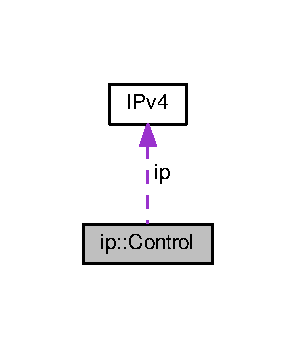
\includegraphics[width=142pt]{structip_1_1Control__coll__graph}
\end{center}
\end{figure}
\subsection*{Public Member Functions}
\begin{DoxyCompactItemize}
\item 
\hyperlink{structip_1_1Control_a0face8d8ee8eb1362440a04f9a6ce4a5}{Control} ()
\begin{DoxyCompactList}\small\item\em Default constructor. \end{DoxyCompactList}\item 
\hyperlink{structip_1_1Control_a32ecd23afdfd205d5b7c7fb780f918ae}{Control} (\hyperlink{namespaceip_a341d8827cf57ab044a78c05922bea473}{Ctrl} c)
\begin{DoxyCompactList}\small\item\em Constructor from \hyperlink{namespaceip_a341d8827cf57ab044a78c05922bea473}{ip\+::\+Ctrl}. \end{DoxyCompactList}\item 
\hyperlink{structip_1_1Control_a082e14e4b06f64d456fb417656ec5f73}{Control} (const \hyperlink{structip_1_1Control}{Control} \&o)
\begin{DoxyCompactList}\small\item\em Copy constructor. \end{DoxyCompactList}\end{DoxyCompactItemize}
\subsection*{Public Attributes}
\begin{DoxyCompactItemize}
\item 
\hyperlink{namespaceip_a341d8827cf57ab044a78c05922bea473}{Ctrl} {\bfseries request}\hypertarget{structip_1_1Control_a4d825322ee770bf17c4921947bb98bc6}{}\label{structip_1_1Control_a4d825322ee770bf17c4921947bb98bc6}

\item 
\hyperlink{structIPv4}{I\+Pv4} {\bfseries ip}\hypertarget{structip_1_1Control_aa8de1b05503ff62f1af2032c8d1861e5}{}\label{structip_1_1Control_aa8de1b05503ff62f1af2032c8d1861e5}

\end{DoxyCompactItemize}


\subsection{Detailed Description}
This struct is used to send control messages to the U\+DP protocol in the near up layer. 

\begin{DoxyAuthor}{Author}
Laouen Louan Mayal Belloli 
\end{DoxyAuthor}
\begin{DoxyDate}{Date}
14 May 2017 
\end{DoxyDate}


\subsection{Constructor \& Destructor Documentation}
\index{ip\+::\+Control@{ip\+::\+Control}!Control@{Control}}
\index{Control@{Control}!ip\+::\+Control@{ip\+::\+Control}}
\subsubsection[{\texorpdfstring{Control()}{Control()}}]{\setlength{\rightskip}{0pt plus 5cm}ip\+::\+Control\+::\+Control (
\begin{DoxyParamCaption}
{}
\end{DoxyParamCaption}
)\hspace{0.3cm}{\ttfamily [inline]}}\hypertarget{structip_1_1Control_a0face8d8ee8eb1362440a04f9a6ce4a5}{}\label{structip_1_1Control_a0face8d8ee8eb1362440a04f9a6ce4a5}


Default constructor. 

Construct a new empty instance. \index{ip\+::\+Control@{ip\+::\+Control}!Control@{Control}}
\index{Control@{Control}!ip\+::\+Control@{ip\+::\+Control}}
\subsubsection[{\texorpdfstring{Control(\+Ctrl c)}{Control(Ctrl c)}}]{\setlength{\rightskip}{0pt plus 5cm}ip\+::\+Control\+::\+Control (
\begin{DoxyParamCaption}
\item[{{\bf Ctrl}}]{c}
\end{DoxyParamCaption}
)\hspace{0.3cm}{\ttfamily [inline]}}\hypertarget{structip_1_1Control_a32ecd23afdfd205d5b7c7fb780f918ae}{}\label{structip_1_1Control_a32ecd23afdfd205d5b7c7fb780f918ae}


Constructor from \hyperlink{namespaceip_a341d8827cf57ab044a78c05922bea473}{ip\+::\+Ctrl}. 

Construct a new instance with the request passed as parameter.


\begin{DoxyParams}{Parameters}
{\em c} & The \hyperlink{namespaceip_a341d8827cf57ab044a78c05922bea473}{ip\+::\+Ctrl} with the request value. \\
\hline
\end{DoxyParams}
\index{ip\+::\+Control@{ip\+::\+Control}!Control@{Control}}
\index{Control@{Control}!ip\+::\+Control@{ip\+::\+Control}}
\subsubsection[{\texorpdfstring{Control(const Control \&o)}{Control(const Control &o)}}]{\setlength{\rightskip}{0pt plus 5cm}ip\+::\+Control\+::\+Control (
\begin{DoxyParamCaption}
\item[{const {\bf Control} \&}]{o}
\end{DoxyParamCaption}
)\hspace{0.3cm}{\ttfamily [inline]}}\hypertarget{structip_1_1Control_a082e14e4b06f64d456fb417656ec5f73}{}\label{structip_1_1Control_a082e14e4b06f64d456fb417656ec5f73}


Copy constructor. 

Construct a new instance from a copy of the one passed as parameter.


\begin{DoxyParams}{Parameters}
{\em o} & The \hyperlink{structip_1_1Control}{ip\+::\+Control} to copy in the new instance. \\
\hline
\end{DoxyParams}


The documentation for this struct was generated from the following file\+:\begin{DoxyCompactItemize}
\item 
/home/lao/\+Documents/git/\+Network\+D\+E\+V\+S/structures/ip.\+h\end{DoxyCompactItemize}

\hypertarget{structlink_1_1Control}{}\section{link\+:\+:Control Struct Reference}
\label{structlink_1_1Control}\index{link\+::\+Control@{link\+::\+Control}}


This struct is used to allow comunication between the io layer and ther link layer.  




{\ttfamily \#include $<$link.\+h$>$}



Collaboration diagram for link\+:\+:Control\+:\nopagebreak
\begin{figure}[H]
\begin{center}
\leavevmode
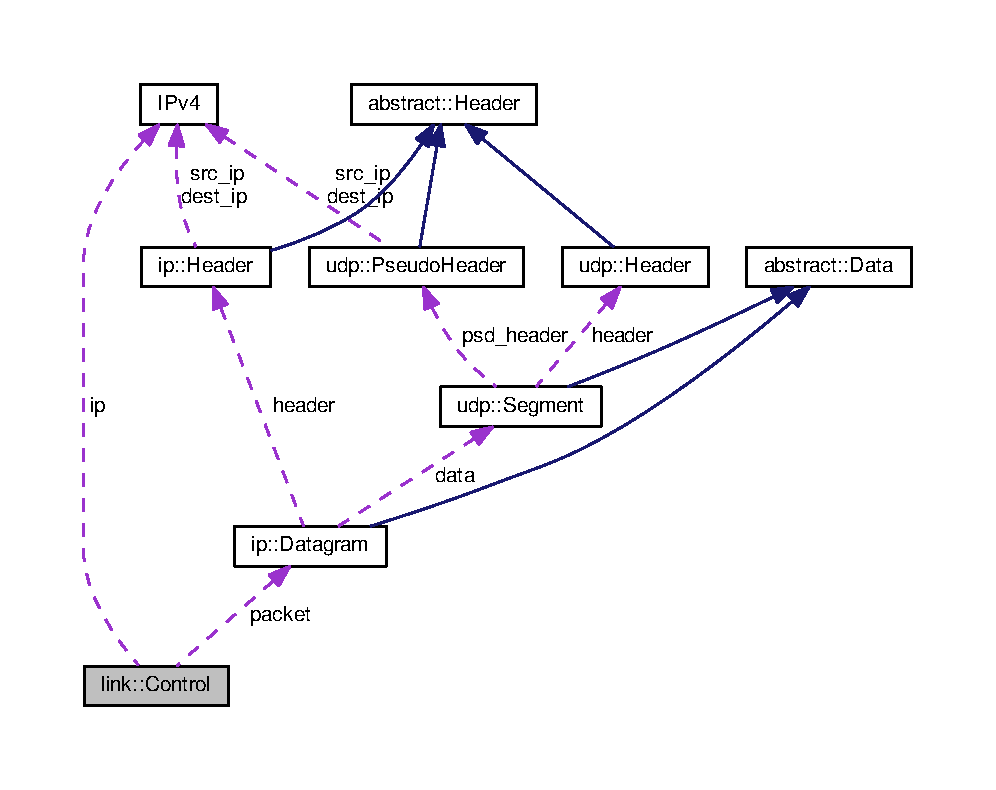
\includegraphics[width=350pt]{structlink_1_1Control__coll__graph}
\end{center}
\end{figure}
\subsection*{Public Member Functions}
\begin{DoxyCompactItemize}
\item 
\hyperlink{structlink_1_1Control_a516338434f0fb973c8f790e8aba08ec6}{Control} ()
\begin{DoxyCompactList}\small\item\em Default constructor. \end{DoxyCompactList}\item 
\hyperlink{structlink_1_1Control_af69072be879940dcb70c80cc40f2e46a}{Control} (const \hyperlink{structlink_1_1Control}{Control} \&other)
\begin{DoxyCompactList}\small\item\em Copy constructor. \end{DoxyCompactList}\end{DoxyCompactItemize}
\subsection*{Public Attributes}
\begin{DoxyCompactItemize}
\item 
Ctrl {\bfseries request}\hypertarget{structlink_1_1Control_afb4bed2321bc90a524872e03126342e9}{}\label{structlink_1_1Control_afb4bed2321bc90a524872e03126342e9}

\item 
ushort {\bfseries interface}\hypertarget{structlink_1_1Control_a9ad3f2480082b69e5b8ab59c4f04c6a3}{}\label{structlink_1_1Control_a9ad3f2480082b69e5b8ab59c4f04c6a3}

\item 
\hyperlink{structIPv4}{I\+Pv4} {\bfseries ip}\hypertarget{structlink_1_1Control_a0b7fcf55d5c517914373a1979fc87277}{}\label{structlink_1_1Control_a0b7fcf55d5c517914373a1979fc87277}

\item 
\hyperlink{structip_1_1Datagram}{ip\+::\+Datagram} {\bfseries packet}\hypertarget{structlink_1_1Control_aa67780caf362cd49f34b9357a2d86999}{}\label{structlink_1_1Control_aa67780caf362cd49f34b9357a2d86999}

\end{DoxyCompactItemize}


\subsection{Detailed Description}
This struct is used to allow comunication between the io layer and ther link layer. 

\begin{DoxyAuthor}{Author}
Laouen Louan Mayal Belloli 
\end{DoxyAuthor}
\begin{DoxyDate}{Date}
14 May 2017
\end{DoxyDate}
A \hyperlink{structlink_1_1Control}{link\+::\+Control} has the next fields\+:
\begin{DoxyEnumerate}
\item request\+: a link\+::\+Ctrol that indicates the purpose of the message.
\item interface\+: an unsigned short that indicate the interface where is conected the link module that is being part of the comunication process.
\item ip\+: If the request is link\+::\+Ctrl\+::\+A\+R\+P\+\_\+\+Q\+U\+E\+RY, this fields contains the ip to ve resolved.
\item packet\+: If the request is link\+::\+Ctrl\+::\+S\+E\+N\+D\+\_\+\+P\+A\+C\+K\+ET, this fields contains the \hyperlink{structip_1_1Datagram}{ip\+::\+Datagram} to send. 
\end{DoxyEnumerate}

\subsection{Constructor \& Destructor Documentation}
\index{link\+::\+Control@{link\+::\+Control}!Control@{Control}}
\index{Control@{Control}!link\+::\+Control@{link\+::\+Control}}
\subsubsection[{\texorpdfstring{Control()}{Control()}}]{\setlength{\rightskip}{0pt plus 5cm}link\+::\+Control\+::\+Control (
\begin{DoxyParamCaption}
{}
\end{DoxyParamCaption}
)\hspace{0.3cm}{\ttfamily [inline]}}\hypertarget{structlink_1_1Control_a516338434f0fb973c8f790e8aba08ec6}{}\label{structlink_1_1Control_a516338434f0fb973c8f790e8aba08ec6}


Default constructor. 

Construct a new empty instance. \index{link\+::\+Control@{link\+::\+Control}!Control@{Control}}
\index{Control@{Control}!link\+::\+Control@{link\+::\+Control}}
\subsubsection[{\texorpdfstring{Control(const Control \&other)}{Control(const Control &other)}}]{\setlength{\rightskip}{0pt plus 5cm}link\+::\+Control\+::\+Control (
\begin{DoxyParamCaption}
\item[{const {\bf Control} \&}]{other}
\end{DoxyParamCaption}
)\hspace{0.3cm}{\ttfamily [inline]}}\hypertarget{structlink_1_1Control_af69072be879940dcb70c80cc40f2e46a}{}\label{structlink_1_1Control_af69072be879940dcb70c80cc40f2e46a}


Copy constructor. 

Construct a copy of the instance passed as parameter in the new instance.


\begin{DoxyParams}{Parameters}
{\em other} & The \hyperlink{structlink_1_1Control}{link\+::\+Control} to copy in the new instance. \\
\hline
\end{DoxyParams}


The documentation for this struct was generated from the following file\+:\begin{DoxyCompactItemize}
\item 
/home/lao/powerdevs/atomics/\+Network\+D\+E\+V\+S/structures/link.\+h\end{DoxyCompactItemize}

\hypertarget{structudp_1_1Control}{}\section{udp\+:\+:Control Struct Reference}
\label{structudp_1_1Control}\index{udp\+::\+Control@{udp\+::\+Control}}


Inheritance diagram for udp\+:\+:Control\+:\nopagebreak
\begin{figure}[H]
\begin{center}
\leavevmode
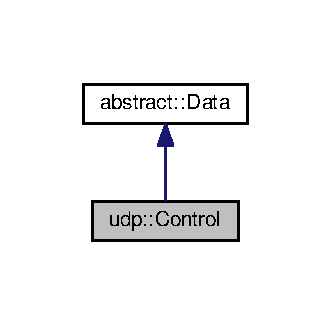
\includegraphics[width=159pt]{structudp_1_1Control__inherit__graph}
\end{center}
\end{figure}


Collaboration diagram for udp\+:\+:Control\+:
\nopagebreak
\begin{figure}[H]
\begin{center}
\leavevmode
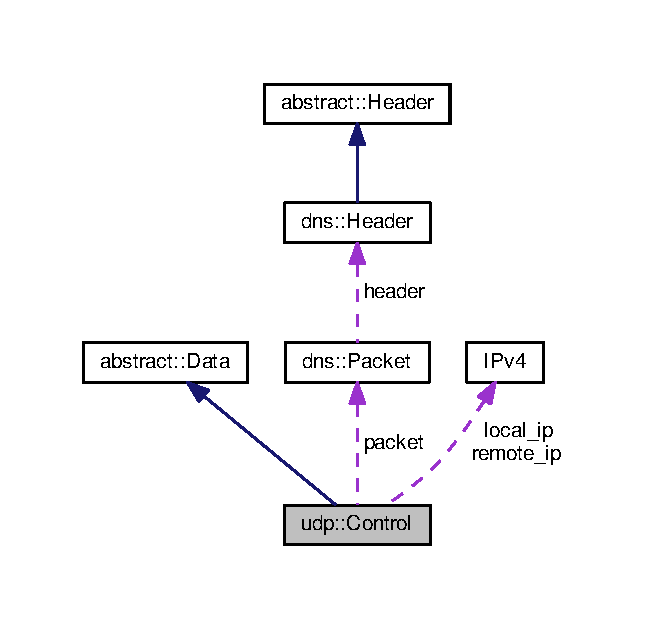
\includegraphics[width=310pt]{structudp_1_1Control__coll__graph}
\end{center}
\end{figure}
\subsection*{Public Member Functions}
\begin{DoxyCompactItemize}
\item 
{\bfseries Control} (const \hyperlink{structudp_1_1Control}{Control} \&other)\hypertarget{structudp_1_1Control_a80ead121f346f13f0541ebc2b8d5e85c}{}\label{structudp_1_1Control_a80ead121f346f13f0541ebc2b8d5e85c}

\item 
{\bfseries Control} (unsigned int other\+\_\+app\+\_\+id, Ctrl other\+\_\+request)\hypertarget{structudp_1_1Control_a52fc45d985e82b72f2866315400db2a7}{}\label{structudp_1_1Control_a52fc45d985e82b72f2866315400db2a7}

\item 
bool {\bfseries is\+App\+Request} () const \hypertarget{structudp_1_1Control_aca09c51711169fbe9631531e80d3c8b6}{}\label{structudp_1_1Control_aca09c51711169fbe9631531e80d3c8b6}

\item 
std\+::string {\bfseries as\+\_\+string} () const \hypertarget{structudp_1_1Control_ad1fcb10d98b4f729bdf6bd54949940d4}{}\label{structudp_1_1Control_ad1fcb10d98b4f729bdf6bd54949940d4}

\end{DoxyCompactItemize}
\subsection*{Public Attributes}
\begin{DoxyCompactItemize}
\item 
Ctrl {\bfseries request}\hypertarget{structudp_1_1Control_a2aa019b350db9c5f2d66f20772d9b79b}{}\label{structudp_1_1Control_a2aa019b350db9c5f2d66f20772d9b79b}

\item 
unsigned int {\bfseries app\+\_\+id}\hypertarget{structudp_1_1Control_af8d12ad139541466d82bd99d79e3be42}{}\label{structudp_1_1Control_af8d12ad139541466d82bd99d79e3be42}

\item 
\hyperlink{structdns_1_1Packet}{dns\+::\+Packet} {\bfseries packet}\hypertarget{structudp_1_1Control_afb69653a07aa874b2c6be07621744c9d}{}\label{structudp_1_1Control_afb69653a07aa874b2c6be07621744c9d}

\item 
ushort {\bfseries local\+\_\+port}\hypertarget{structudp_1_1Control_a4f07eed648f80d37385c12a0b5b803f8}{}\label{structudp_1_1Control_a4f07eed648f80d37385c12a0b5b803f8}

\item 
ushort {\bfseries remote\+\_\+port}\hypertarget{structudp_1_1Control_a03d29c28ed03e44e4db2df155f638b3e}{}\label{structudp_1_1Control_a03d29c28ed03e44e4db2df155f638b3e}

\item 
\hyperlink{structIPv4}{I\+Pv4} {\bfseries local\+\_\+ip}\hypertarget{structudp_1_1Control_a3f31765e13cd17a0c2661754971db196}{}\label{structudp_1_1Control_a3f31765e13cd17a0c2661754971db196}

\item 
\hyperlink{structIPv4}{I\+Pv4} {\bfseries remote\+\_\+ip}\hypertarget{structudp_1_1Control_ae07465d93c71c8ed4a74d8c523c6f054}{}\label{structudp_1_1Control_ae07465d93c71c8ed4a74d8c523c6f054}

\end{DoxyCompactItemize}


The documentation for this struct was generated from the following file\+:\begin{DoxyCompactItemize}
\item 
/home/lao/powerdevs/atomics/\+Network\+D\+E\+V\+S/structures/udp.\+h\end{DoxyCompactItemize}

\hypertarget{structabstract_1_1Data}{}\section{abstract\+:\+:Data Struct Reference}
\label{structabstract_1_1Data}\index{abstract\+::\+Data@{abstract\+::\+Data}}


Represent an abstract data structure for any kind of network data.  




{\ttfamily \#include $<$abstract\+\_\+types.\+h$>$}



Inheritance diagram for abstract\+:\+:Data\+:\nopagebreak
\begin{figure}[H]
\begin{center}
\leavevmode
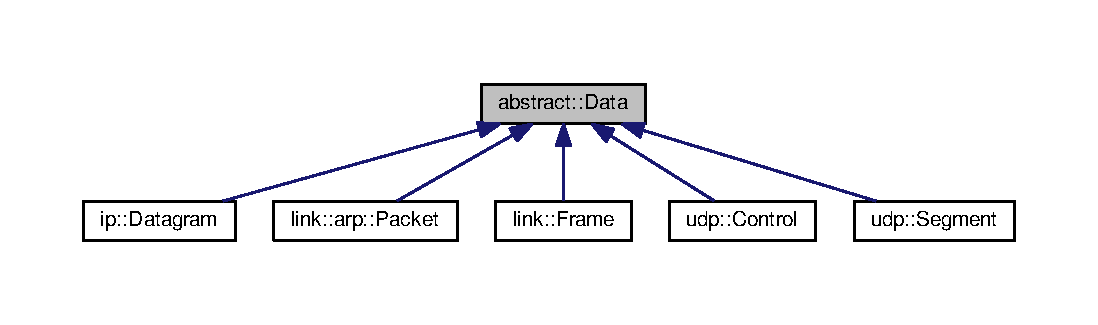
\includegraphics[width=350pt]{structabstract_1_1Data__inherit__graph}
\end{center}
\end{figure}


\subsection{Detailed Description}
Represent an abstract data structure for any kind of network data. 

\begin{DoxyAuthor}{Author}
Laouen Louan Mayal Belloli 
\end{DoxyAuthor}
\begin{DoxyDate}{Date}
14 May 2017
\end{DoxyDate}
This struct it is used to clasify the structs into header and data. It does not implement any functionality. 

The documentation for this struct was generated from the following file\+:\begin{DoxyCompactItemize}
\item 
/home/lao/powerdevs/atomics/\+Network\+D\+E\+V\+S/structures/abstract\+\_\+types.\+h\end{DoxyCompactItemize}

\hypertarget{structip_1_1Datagram}{}\section{ip\+:\+:Datagram Struct Reference}
\label{structip_1_1Datagram}\index{ip\+::\+Datagram@{ip\+::\+Datagram}}


Inheritance diagram for ip\+:\+:Datagram\+:\nopagebreak
\begin{figure}[H]
\begin{center}
\leavevmode
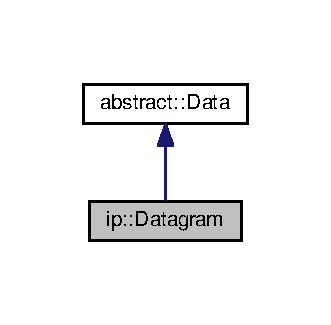
\includegraphics[width=159pt]{structip_1_1Datagram__inherit__graph}
\end{center}
\end{figure}


Collaboration diagram for ip\+:\+:Datagram\+:\nopagebreak
\begin{figure}[H]
\begin{center}
\leavevmode
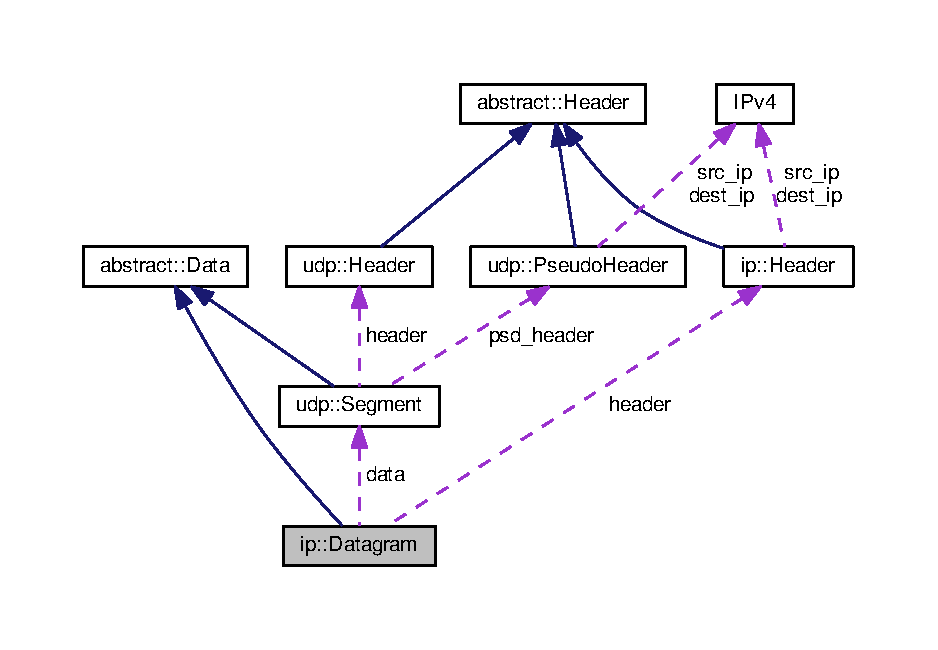
\includegraphics[width=350pt]{structip_1_1Datagram__coll__graph}
\end{center}
\end{figure}
\subsection*{Public Member Functions}
\begin{DoxyCompactItemize}
\item 
{\bfseries Datagram} (const \hyperlink{structip_1_1Datagram}{Datagram} \&other)\hypertarget{structip_1_1Datagram_a9b701e9ceeeacc10ae5df56bccde8f51}{}\label{structip_1_1Datagram_a9b701e9ceeeacc10ae5df56bccde8f51}

\end{DoxyCompactItemize}
\subsection*{Public Attributes}
\begin{DoxyCompactItemize}
\item 
\hyperlink{structip_1_1Header}{Header} {\bfseries header}\hypertarget{structip_1_1Datagram_ab2f6057ca4c00b3c1d9637a5e7b6c144}{}\label{structip_1_1Datagram_ab2f6057ca4c00b3c1d9637a5e7b6c144}

\item 
\hyperlink{structudp_1_1Segment}{udp\+::\+Segment} {\bfseries data}\hypertarget{structip_1_1Datagram_a4de3ad46fa81bc6d312c2e77321e59d1}{}\label{structip_1_1Datagram_a4de3ad46fa81bc6d312c2e77321e59d1}

\end{DoxyCompactItemize}


The documentation for this struct was generated from the following file\+:\begin{DoxyCompactItemize}
\item 
/home/lao/powerdevs/atomics/\+Network\+D\+E\+V\+S/structures/ip.\+h\end{DoxyCompactItemize}

\hypertarget{classdemultiplexer}{}\section{demultiplexer$<$ M\+SG $>$ Class Template Reference}
\label{classdemultiplexer}\index{demultiplexer$<$ M\+S\+G $>$@{demultiplexer$<$ M\+S\+G $>$}}


Template meta model of a demultiplexer that receives a message\+::multiplexed$<$\+M\+S\+G$>$ in the input port number zero and returns the encapsulated message through the port indicated by the interface field of the multiplexed instance.  




{\ttfamily \#include $<$demultiplexer.\+h$>$}



Inheritance diagram for demultiplexer$<$ M\+SG $>$\+:\nopagebreak
\begin{figure}[H]
\begin{center}
\leavevmode
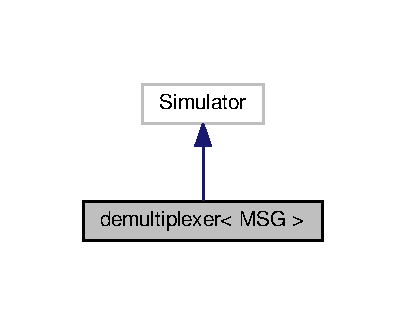
\includegraphics[width=195pt]{classdemultiplexer__inherit__graph}
\end{center}
\end{figure}


Collaboration diagram for demultiplexer$<$ M\+SG $>$\+:\nopagebreak
\begin{figure}[H]
\begin{center}
\leavevmode
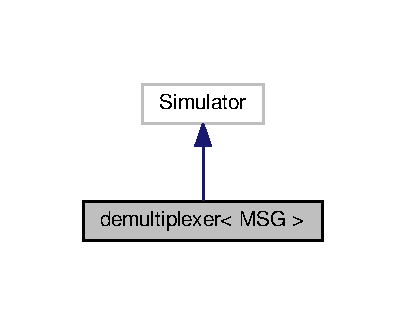
\includegraphics[width=195pt]{classdemultiplexer__coll__graph}
\end{center}
\end{figure}
\subsection*{Public Member Functions}
\begin{DoxyCompactItemize}
\item 
{\bfseries demultiplexer} (const char $\ast$n)\hypertarget{classdemultiplexer_ac0ffa1eb3ce7caac3f20f3908d7d819d}{}\label{classdemultiplexer_ac0ffa1eb3ce7caac3f20f3908d7d819d}

\item 
void {\bfseries init} (double t,...)\hypertarget{classdemultiplexer_ac7c93289875df74e1dfcd2175df19166}{}\label{classdemultiplexer_ac7c93289875df74e1dfcd2175df19166}

\item 
double {\bfseries ta} (double t)\hypertarget{classdemultiplexer_a4c7cc8b523b116010118d564ef8a4d8a}{}\label{classdemultiplexer_a4c7cc8b523b116010118d564ef8a4d8a}

\item 
void {\bfseries dint} (double t)\hypertarget{classdemultiplexer_a4921af7a5202a37af68b1b2197cc3285}{}\label{classdemultiplexer_a4921af7a5202a37af68b1b2197cc3285}

\item 
void {\bfseries dext} (Event x, double t)\hypertarget{classdemultiplexer_aae8739a52134e736f3fab5719518ba74}{}\label{classdemultiplexer_aae8739a52134e736f3fab5719518ba74}

\item 
Event {\bfseries lambda} (double t)\hypertarget{classdemultiplexer_a8fdbd39d23564293c263a42a9513392d}{}\label{classdemultiplexer_a8fdbd39d23564293c263a42a9513392d}

\item 
void {\bfseries exit} ()\hypertarget{classdemultiplexer_a201e20cca9a7d603d3373ca7053e6b7d}{}\label{classdemultiplexer_a201e20cca9a7d603d3373ca7053e6b7d}

\end{DoxyCompactItemize}


\subsection{Detailed Description}
\subsubsection*{template$<$typename M\+SG$>$\\*
class demultiplexer$<$ M\+S\+G $>$}

Template meta model of a demultiplexer that receives a message\+::multiplexed$<$\+M\+S\+G$>$ in the input port number zero and returns the encapsulated message through the port indicated by the interface field of the multiplexed instance. 

\begin{DoxyAuthor}{Author}
Laouen Louan Mayal Belloli 
\end{DoxyAuthor}
\begin{DoxyDate}{Date}
14 May 2017
\end{DoxyDate}
This model must be inherited by a new class with the template M\+SG parameter specified with the same data type that is specified in the message\+::multiplexed type that will arrives to this model.

The new class must follow the Power\+D\+E\+VS specifications and a .cpp file must exist even if it is an empty file in order to correctly compile the model from the Power\+D\+E\+VS I\+DE.

The next rules must be followed\+:
\begin{DoxyEnumerate}
\item This file must be included in the file where the new class is declared.
\item The new class name must be all lower case.
\item The new class must have in the first line the next comment\+: //\+C\+PP\+:network\+D\+E\+V\+S/new\+\_\+class\+\_\+name.\+cpp.
\item The file network\+D\+E\+V\+S/new\+\_\+class\+\_\+name.\+cpp must exist as an empty file.
\item The constructor of the new class must be specified in the public section as shown here\+: new\+\_\+class\+\_\+name(const char $\ast$n)\+: \hyperlink{classdemultiplexer}{demultiplexer(n)} \{\};
\end{DoxyEnumerate}

The parameters to specifie in the Power\+D\+E\+VS I\+DE (right click in the atomic model -\/$>$ edit -\/$>$ parameters) are the nexts\+:

\tabulinesep=1mm
\begin{longtabu} spread 0pt [c]{*3{|X[-1]}|}
\hline
\rowcolor{\tableheadbgcolor}\PBS\centering {\bf name }&\PBS\centering {\bf type }&\PBS\centering {\bf description  }\\\cline{1-3}
\endfirsthead
\hline
\endfoot
\hline
\rowcolor{\tableheadbgcolor}\PBS\centering {\bf name }&\PBS\centering {\bf type }&\PBS\centering {\bf description  }\\\cline{1-3}
\endhead
\PBS\centering module name &\PBS\centering String &\PBS\centering a name used to tag the logs generated by this model \\\cline{1-3}
\end{longtabu}

\begin{DoxyTemplParams}{Template Parameters}
{\em M\+SG} & The data type of the template parameter M\+SG of the \hyperlink{structmessage_1_1Multiplexed}{message\+::\+Multiplexed} message that arrives in the input port zero. \\
\hline
\end{DoxyTemplParams}


The documentation for this class was generated from the following file\+:\begin{DoxyCompactItemize}
\item 
/home/lao/powerdevs/atomics/\+Network\+D\+E\+V\+S/template/demultiplexer.\+h\end{DoxyCompactItemize}

\hypertarget{classdemultiplexer__ip__link}{}\section{demultiplexer\+\_\+ip\+\_\+link Class Reference}
\label{classdemultiplexer__ip__link}\index{demultiplexer\+\_\+ip\+\_\+link@{demultiplexer\+\_\+ip\+\_\+link}}


Inheritance diagram for demultiplexer\+\_\+ip\+\_\+link\+:
\nopagebreak
\begin{figure}[H]
\begin{center}
\leavevmode
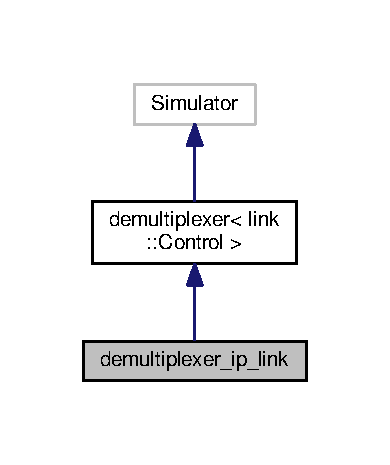
\includegraphics[width=187pt]{classdemultiplexer__ip__link__inherit__graph}
\end{center}
\end{figure}


Collaboration diagram for demultiplexer\+\_\+ip\+\_\+link\+:
\nopagebreak
\begin{figure}[H]
\begin{center}
\leavevmode
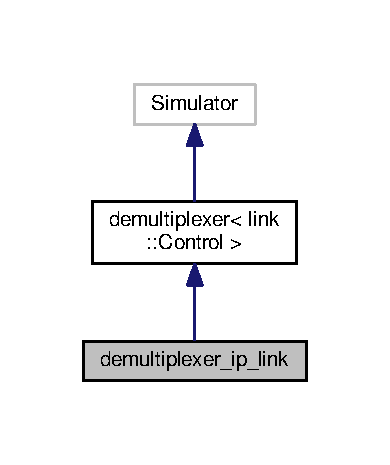
\includegraphics[width=187pt]{classdemultiplexer__ip__link__coll__graph}
\end{center}
\end{figure}
\subsection*{Public Member Functions}
\begin{DoxyCompactItemize}
\item 
{\bfseries demultiplexer\+\_\+ip\+\_\+link} (const char $\ast$n)\hypertarget{classdemultiplexer__ip__link_aec9879ae23d1a8c51d7d73f9c8b3e2a5}{}\label{classdemultiplexer__ip__link_aec9879ae23d1a8c51d7d73f9c8b3e2a5}

\end{DoxyCompactItemize}


The documentation for this class was generated from the following file\+:\begin{DoxyCompactItemize}
\item 
/home/lao/powerdevs/atomics/\+Network\+D\+E\+V\+S/demultiplexer\+\_\+ip\+\_\+link.\+h\end{DoxyCompactItemize}

\hypertarget{classdemultiplexer__switch}{}\section{demultiplexer\+\_\+switch Class Reference}
\label{classdemultiplexer__switch}\index{demultiplexer\+\_\+switch@{demultiplexer\+\_\+switch}}


A specialization of the \hyperlink{classdemultiplexer}{demultiplexer} template model to demultiplex message\+::\+Multiplexed$<$link\+::\+Frame$>$ messages.  




{\ttfamily \#include $<$demultiplexer\+\_\+switch.\+h$>$}



Inheritance diagram for demultiplexer\+\_\+switch\+:\nopagebreak
\begin{figure}[H]
\begin{center}
\leavevmode
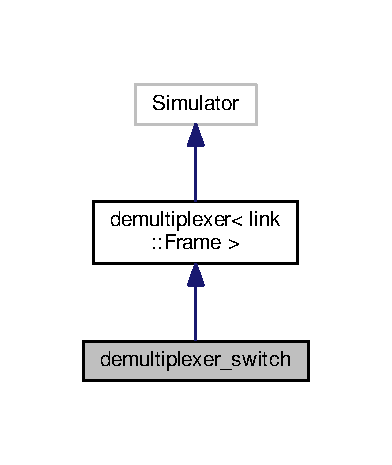
\includegraphics[width=188pt]{classdemultiplexer__switch__inherit__graph}
\end{center}
\end{figure}


Collaboration diagram for demultiplexer\+\_\+switch\+:\nopagebreak
\begin{figure}[H]
\begin{center}
\leavevmode
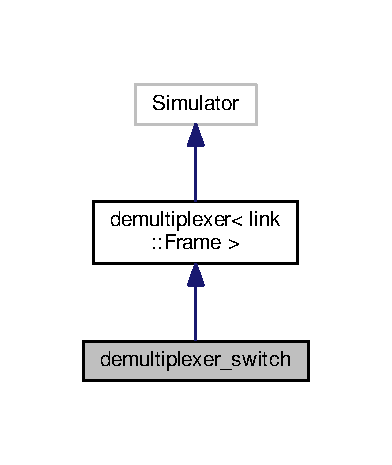
\includegraphics[width=188pt]{classdemultiplexer__switch__coll__graph}
\end{center}
\end{figure}
\subsection*{Public Member Functions}
\begin{DoxyCompactItemize}
\item 
{\bfseries demultiplexer\+\_\+switch} (const char $\ast$n)\hypertarget{classdemultiplexer__switch_a7e1728adcdcb9628a53c66e2c2e8ad3d}{}\label{classdemultiplexer__switch_a7e1728adcdcb9628a53c66e2c2e8ad3d}

\end{DoxyCompactItemize}


\subsection{Detailed Description}
A specialization of the \hyperlink{classdemultiplexer}{demultiplexer} template model to demultiplex message\+::\+Multiplexed$<$link\+::\+Frame$>$ messages. 

\begin{DoxyAuthor}{Author}
Lauen Louan Mayal Belloli 
\end{DoxyAuthor}
\begin{DoxyDate}{Date}
14 May 2017 
\end{DoxyDate}


The documentation for this class was generated from the following file\+:\begin{DoxyCompactItemize}
\item 
/home/lao/powerdevs/atomics/\+Network\+D\+E\+V\+S/demultiplexer\+\_\+switch.\+h\end{DoxyCompactItemize}

\hypertarget{classdns__packet__sink}{}\section{dns\+\_\+packet\+\_\+sink Class Reference}
\label{classdns__packet__sink}\index{dns\+\_\+packet\+\_\+sink@{dns\+\_\+packet\+\_\+sink}}


A specialization of \hyperlink{classoutput__stream}{output\+\_\+stream} template model to write in a file output messages of type \hyperlink{structdns_1_1Packet}{dns\+::\+Packet}.  




{\ttfamily \#include $<$dns\+\_\+packet\+\_\+sink.\+h$>$}



Inheritance diagram for dns\+\_\+packet\+\_\+sink\+:\nopagebreak
\begin{figure}[H]
\begin{center}
\leavevmode
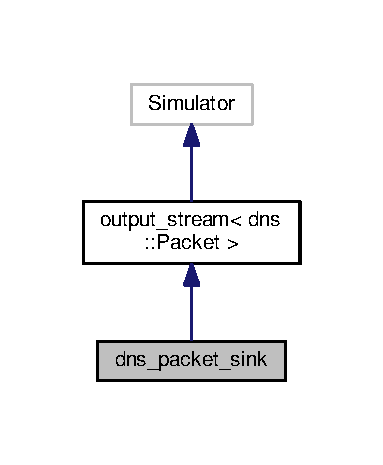
\includegraphics[width=184pt]{classdns__packet__sink__inherit__graph}
\end{center}
\end{figure}


Collaboration diagram for dns\+\_\+packet\+\_\+sink\+:\nopagebreak
\begin{figure}[H]
\begin{center}
\leavevmode
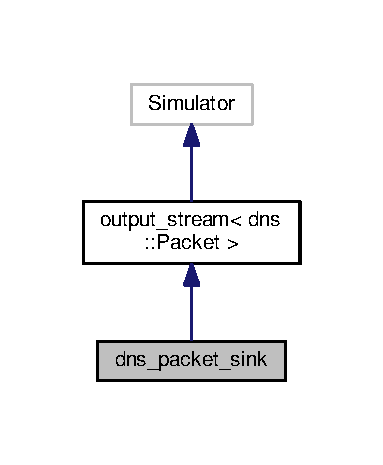
\includegraphics[width=184pt]{classdns__packet__sink__coll__graph}
\end{center}
\end{figure}
\subsection*{Public Member Functions}
\begin{DoxyCompactItemize}
\item 
{\bfseries dns\+\_\+packet\+\_\+sink} (const char $\ast$n)\hypertarget{classdns__packet__sink_a2ead1895f1847c995f3bed2c10fe52e9}{}\label{classdns__packet__sink_a2ead1895f1847c995f3bed2c10fe52e9}

\end{DoxyCompactItemize}


\subsection{Detailed Description}
A specialization of \hyperlink{classoutput__stream}{output\+\_\+stream} template model to write in a file output messages of type \hyperlink{structdns_1_1Packet}{dns\+::\+Packet}. 

\begin{DoxyAuthor}{Author}
Lauen Louan Mayal Belloli 
\end{DoxyAuthor}
\begin{DoxyDate}{Date}
14 May 2017 
\end{DoxyDate}


The documentation for this class was generated from the following file\+:\begin{DoxyCompactItemize}
\item 
/home/lao/powerdevs/atomics/\+Network\+D\+E\+V\+S/dns\+\_\+packet\+\_\+sink.\+h\end{DoxyCompactItemize}

\hypertarget{classdns__packet__src}{}\section{dns\+\_\+packet\+\_\+src Class Reference}
\label{classdns__packet__src}\index{dns\+\_\+packet\+\_\+src@{dns\+\_\+packet\+\_\+src}}


A specialization of \hyperlink{classinput__stream}{input\+\_\+stream} template model to generate input of type \hyperlink{structdns_1_1Packet}{dns\+::\+Packet} from a file.  




{\ttfamily \#include $<$dns\+\_\+packet\+\_\+src.\+h$>$}



Inheritance diagram for dns\+\_\+packet\+\_\+src\+:\nopagebreak
\begin{figure}[H]
\begin{center}
\leavevmode
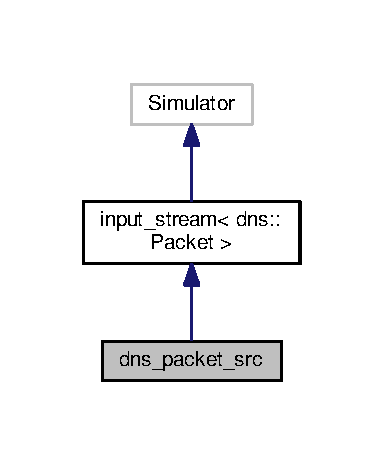
\includegraphics[width=184pt]{classdns__packet__src__inherit__graph}
\end{center}
\end{figure}


Collaboration diagram for dns\+\_\+packet\+\_\+src\+:\nopagebreak
\begin{figure}[H]
\begin{center}
\leavevmode
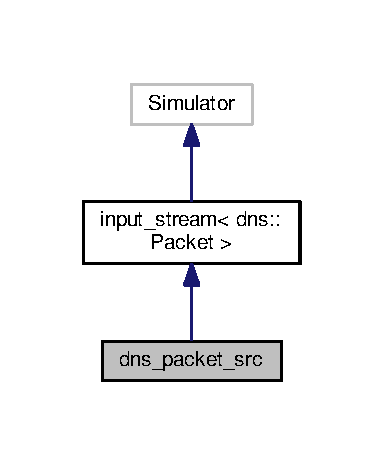
\includegraphics[width=184pt]{classdns__packet__src__coll__graph}
\end{center}
\end{figure}
\subsection*{Public Member Functions}
\begin{DoxyCompactItemize}
\item 
{\bfseries dns\+\_\+packet\+\_\+src} (const char $\ast$n)\hypertarget{classdns__packet__src_a6b057e9ffb6aa7fbbf52262e34a6d85c}{}\label{classdns__packet__src_a6b057e9ffb6aa7fbbf52262e34a6d85c}

\end{DoxyCompactItemize}


\subsection{Detailed Description}
A specialization of \hyperlink{classinput__stream}{input\+\_\+stream} template model to generate input of type \hyperlink{structdns_1_1Packet}{dns\+::\+Packet} from a file. 

\begin{DoxyAuthor}{Author}
Lauen Louan Mayal Belloli 
\end{DoxyAuthor}
\begin{DoxyDate}{Date}
14 May 2017 
\end{DoxyDate}


The documentation for this class was generated from the following file\+:\begin{DoxyCompactItemize}
\item 
/home/lao/powerdevs/atomics/\+Network\+D\+E\+V\+S/dns\+\_\+packet\+\_\+src.\+h\end{DoxyCompactItemize}

\hypertarget{classdns__server}{}\section{dns\+\_\+server Class Reference}
\label{classdns__server}\index{dns\+\_\+server@{dns\+\_\+server}}


Inheritance diagram for dns\+\_\+server\+:\nopagebreak
\begin{figure}[H]
\begin{center}
\leavevmode
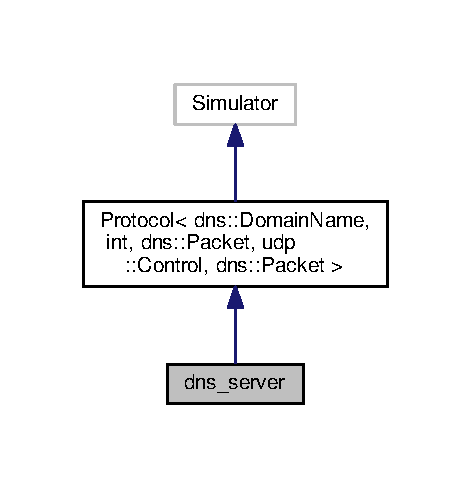
\includegraphics[width=214pt]{classdns__server__inherit__graph}
\end{center}
\end{figure}


Collaboration diagram for dns\+\_\+server\+:\nopagebreak
\begin{figure}[H]
\begin{center}
\leavevmode
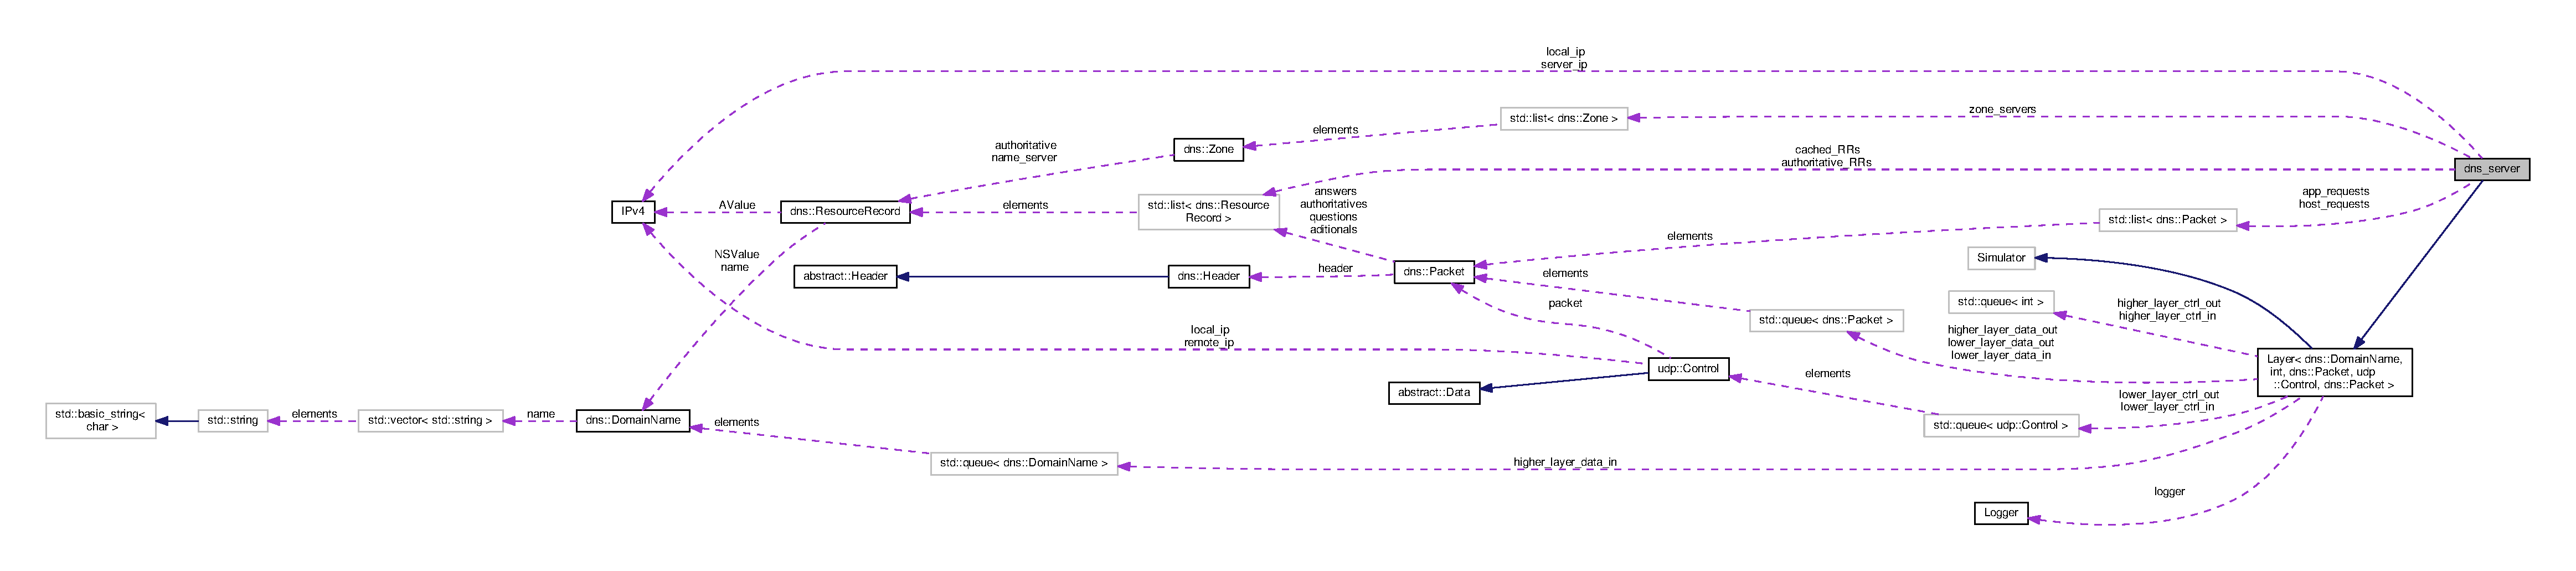
\includegraphics[width=350pt]{classdns__server__coll__graph}
\end{center}
\end{figure}
\subsection*{Public Member Functions}
\begin{DoxyCompactItemize}
\item 
{\bfseries dns\+\_\+server} (const char $\ast$n)\hypertarget{classdns__server_afbeb3f646717cf7960d54385e469b850}{}\label{classdns__server_afbeb3f646717cf7960d54385e469b850}

\item 
void {\bfseries init} (double,...)\hypertarget{classdns__server_a4b17d2d96b3e7a702495b8f44707ec02}{}\label{classdns__server_a4b17d2d96b3e7a702495b8f44707ec02}

\item 
double {\bfseries ta} (double t)\hypertarget{classdns__server_a18ec5017d2e817ddf8d876b3f3f747e5}{}\label{classdns__server_a18ec5017d2e817ddf8d876b3f3f747e5}

\item 
Event {\bfseries lambda} (double)\hypertarget{classdns__server_ad691a03c4bfb71509b3043560c6b73b0}{}\label{classdns__server_ad691a03c4bfb71509b3043560c6b73b0}

\item 
void {\bfseries exit} ()\hypertarget{classdns__server_a05eb620b2f8308ec3818cf5412669890}{}\label{classdns__server_a05eb620b2f8308ec3818cf5412669890}

\item 
virtual void \hyperlink{classdns__server_a51e296892a2de8776c83689f172a0797}{dinternal} (double)
\begin{DoxyCompactList}\small\item\em This method is virtual and must be overloaded with the protocol. \end{DoxyCompactList}\item 
virtual void \hyperlink{classdns__server_a3a6cdeea496be969d034af8a0bdb893f}{dexternal} (double)
\begin{DoxyCompactList}\small\item\em This method is virtual and can be overloaded with the protocol. \end{DoxyCompactList}\end{DoxyCompactItemize}
\subsection*{Protected Member Functions}
\begin{DoxyCompactItemize}
\item 
void {\bfseries process\+Domain\+Name} (\hyperlink{structdns_1_1DomainName}{dns\+::\+Domain\+Name} domain)\hypertarget{classdns__server_ade0acda9d6fc57e25a7a52645101c753}{}\label{classdns__server_ade0acda9d6fc57e25a7a52645101c753}

\item 
void {\bfseries send\+To} (const \hyperlink{structdns_1_1Packet}{dns\+::\+Packet} \&p, \hyperlink{structIPv4}{I\+Pv4} server\+\_\+ip, ushort server\+\_\+port)\hypertarget{classdns__server_a0471cc529b817849b3910a6c8e415a86}{}\label{classdns__server_a0471cc529b817849b3910a6c8e415a86}

\item 
void {\bfseries process\+D\+N\+S\+Packet} (\hyperlink{structdns_1_1Packet}{dns\+::\+Packet} packet)\hypertarget{classdns__server_aedffffa660f9076ce9a5e2ee8de8602d}{}\label{classdns__server_aedffffa660f9076ce9a5e2ee8de8602d}

\item 
void {\bfseries set\+As\+Response} (\hyperlink{structdns_1_1Packet}{dns\+::\+Packet} \&packet)\hypertarget{classdns__server_aa05469d6b169567590aa23b64119e413}{}\label{classdns__server_aa05469d6b169567590aa23b64119e413}

\item 
void {\bfseries direct\+Answer} (\hyperlink{structdns_1_1Packet}{dns\+::\+Packet} \&packet)\hypertarget{classdns__server_a2ed1fc3068bf26f5932f3ba55cc7d374}{}\label{classdns__server_a2ed1fc3068bf26f5932f3ba55cc7d374}

\item 
void {\bfseries deliver\+Answer} (const \hyperlink{structdns_1_1Packet}{dns\+::\+Packet} \&packet)\hypertarget{classdns__server_ac0521c8ec9d0c0283bfcf1e53e1e5bcb}{}\label{classdns__server_ac0521c8ec9d0c0283bfcf1e53e1e5bcb}

\item 
void {\bfseries set\+Authoritative\+Flag} (\hyperlink{structdns_1_1Packet}{dns\+::\+Packet} \&packet, \hyperlink{structdns_1_1DomainName}{dns\+::\+Domain\+Name} d)\hypertarget{classdns__server_af6b289b84e5be96e9596193b06daf65f}{}\label{classdns__server_af6b289b84e5be96e9596193b06daf65f}

\item 
void {\bfseries remove\+Packet} (ushort id)\hypertarget{classdns__server_a29ce34ee3c497ba383b1651498500b12}{}\label{classdns__server_a29ce34ee3c497ba383b1651498500b12}

\item 
\hyperlink{structdns_1_1Packet}{dns\+::\+Packet} {\bfseries get\+Packet} (ushort id)\hypertarget{classdns__server_afcfb30629b4d0538bac2c44f1659d9eb}{}\label{classdns__server_afcfb30629b4d0538bac2c44f1659d9eb}

\item 
void {\bfseries update\+Cache} (double t)\hypertarget{classdns__server_af8c786411d5c0eb9f24f53c928ac9b48}{}\label{classdns__server_af8c786411d5c0eb9f24f53c928ac9b48}

\item 
\hyperlink{structdns_1_1Zone}{dns\+::\+Zone} {\bfseries get\+Best\+Match} (\hyperlink{structdns_1_1DomainName}{dns\+::\+Domain\+Name} d)\hypertarget{classdns__server_a0b1f6f215b752925e9901adf16df7edf}{}\label{classdns__server_a0b1f6f215b752925e9901adf16df7edf}

\item 
\hyperlink{structdns_1_1Packet}{dns\+::\+Packet} {\bfseries Query\+Packet} (\hyperlink{structdns_1_1DomainName}{dns\+::\+Domain\+Name} d)\hypertarget{classdns__server_ac4a4d1569cfb515454b442a2bd0d84db}{}\label{classdns__server_ac4a4d1569cfb515454b442a2bd0d84db}

\item 
bool {\bfseries is\+App\+Request} (ushort id) const \hypertarget{classdns__server_a87c7e3fe0cfa2e0cf4ac452b9dbf05da}{}\label{classdns__server_a87c7e3fe0cfa2e0cf4ac452b9dbf05da}

\item 
bool {\bfseries is\+Host\+Request} (ushort id) const \hypertarget{classdns__server_a86c84b8b2f3e35d546a3ad9660944de9}{}\label{classdns__server_a86c84b8b2f3e35d546a3ad9660944de9}

\item 
bool {\bfseries exist\+RR} (const \hyperlink{structdns_1_1DomainName}{dns\+::\+Domain\+Name} \&d) const \hypertarget{classdns__server_ab0d83fc5df34b863592c906f01e681bc}{}\label{classdns__server_ab0d83fc5df34b863592c906f01e681bc}

\item 
\hyperlink{structdns_1_1ResourceRecord}{dns\+::\+Resource\+Record} {\bfseries get\+RR} (const \hyperlink{structdns_1_1DomainName}{dns\+::\+Domain\+Name} \&d)\hypertarget{classdns__server_a2c2bffe8648fed6274b8fcde47f2f3bd}{}\label{classdns__server_a2c2bffe8648fed6274b8fcde47f2f3bd}

\end{DoxyCompactItemize}
\subsection*{Protected Attributes}
\begin{DoxyCompactItemize}
\item 
int {\bfseries next\+\_\+id}\hypertarget{classdns__server_a2da2838d3660ae78cba549d9acb899e7}{}\label{classdns__server_a2da2838d3660ae78cba549d9acb899e7}

\item 
bool {\bfseries bind}\hypertarget{classdns__server_aa593f877363212c866ffa1fe59a06435}{}\label{classdns__server_aa593f877363212c866ffa1fe59a06435}

\item 
bool {\bfseries start\+\_\+reading}\hypertarget{classdns__server_a9245a53bf6cd3a03fe38b5ef1c08cd1a}{}\label{classdns__server_a9245a53bf6cd3a03fe38b5ef1c08cd1a}

\item 
bool {\bfseries recursive\+\_\+allowed}\hypertarget{classdns__server_a754e1a5b9cc9f5831724d3209fa101e7}{}\label{classdns__server_a754e1a5b9cc9f5831724d3209fa101e7}

\item 
\hyperlink{structIPv4}{I\+Pv4} {\bfseries local\+\_\+ip}\hypertarget{classdns__server_a3b185eef3b7d44822d0a9a12baeb71ee}{}\label{classdns__server_a3b185eef3b7d44822d0a9a12baeb71ee}

\item 
\hyperlink{structIPv4}{I\+Pv4} {\bfseries server\+\_\+ip}\hypertarget{classdns__server_af587511dc4a23c264e30502506746c9a}{}\label{classdns__server_af587511dc4a23c264e30502506746c9a}

\item 
std\+::list$<$ \hyperlink{structdns_1_1ResourceRecord}{dns\+::\+Resource\+Record} $>$ {\bfseries cached\+\_\+\+R\+Rs}\hypertarget{classdns__server_a9708a2ed7f8735caaf541b1fde6ee15d}{}\label{classdns__server_a9708a2ed7f8735caaf541b1fde6ee15d}

\item 
std\+::list$<$ \hyperlink{structdns_1_1ResourceRecord}{dns\+::\+Resource\+Record} $>$ {\bfseries authoritative\+\_\+\+R\+Rs}\hypertarget{classdns__server_aafed2cfadd1263403cf6147981ca503b}{}\label{classdns__server_aafed2cfadd1263403cf6147981ca503b}

\item 
std\+::list$<$ \hyperlink{structdns_1_1Zone}{dns\+::\+Zone} $>$ {\bfseries zone\+\_\+servers}\hypertarget{classdns__server_a4e467dbf292e6f8e15b28fe93c4969fb}{}\label{classdns__server_a4e467dbf292e6f8e15b28fe93c4969fb}

\item 
std\+::list$<$ \hyperlink{structdns_1_1Packet}{dns\+::\+Packet} $>$ {\bfseries app\+\_\+requests}\hypertarget{classdns__server_a4df4c84961c098bba0dcc5fe41e52564}{}\label{classdns__server_a4df4c84961c098bba0dcc5fe41e52564}

\item 
std\+::list$<$ \hyperlink{structdns_1_1Packet}{dns\+::\+Packet} $>$ {\bfseries host\+\_\+requests}\hypertarget{classdns__server_a0ed8a7cc91535c4bbcff5320503dc8ba}{}\label{classdns__server_a0ed8a7cc91535c4bbcff5320503dc8ba}

\item 
double {\bfseries process\+\_\+dns\+\_\+query} = 0.\+001\hypertarget{classdns__server_a9444ae1982f78180dd1c8d905b46d3c3}{}\label{classdns__server_a9444ae1982f78180dd1c8d905b46d3c3}

\item 
double {\bfseries process\+\_\+dns\+\_\+response} = 0.\+001\hypertarget{classdns__server_a5b577ff9d1e88181cd5c753c6ea31c07}{}\label{classdns__server_a5b577ff9d1e88181cd5c753c6ea31c07}

\end{DoxyCompactItemize}


\subsection{Member Function Documentation}
\index{dns\+\_\+server@{dns\+\_\+server}!dexternal@{dexternal}}
\index{dexternal@{dexternal}!dns\+\_\+server@{dns\+\_\+server}}
\subsubsection[{\texorpdfstring{dexternal(double)}{dexternal(double)}}]{\setlength{\rightskip}{0pt plus 5cm}void dns\+\_\+server\+::dexternal (
\begin{DoxyParamCaption}
\item[{double}]{t}
\end{DoxyParamCaption}
)\hspace{0.3cm}{\ttfamily [virtual]}}\hypertarget{classdns__server_a3a6cdeea496be969d034af8a0bdb893f}{}\label{classdns__server_a3a6cdeea496be969d034af8a0bdb893f}


This method is virtual and can be overloaded with the protocol. 

This method is called each time an external transition takes place.


\begin{DoxyParams}{Parameters}
{\em t} & The virtual global time of the simulation at which the method is triggered. \\
\hline
\end{DoxyParams}


Reimplemented from \hyperlink{classLayer_ae21ef24340c6c1f6cf20d66b5ab6a5f7}{Layer$<$ dns\+::\+Domain\+Name, int, dns\+::\+Packet, udp\+::\+Control, dns\+::\+Packet $>$}.

\index{dns\+\_\+server@{dns\+\_\+server}!dinternal@{dinternal}}
\index{dinternal@{dinternal}!dns\+\_\+server@{dns\+\_\+server}}
\subsubsection[{\texorpdfstring{dinternal(double)}{dinternal(double)}}]{\setlength{\rightskip}{0pt plus 5cm}void dns\+\_\+server\+::dinternal (
\begin{DoxyParamCaption}
\item[{double}]{t}
\end{DoxyParamCaption}
)\hspace{0.3cm}{\ttfamily [virtual]}}\hypertarget{classdns__server_a51e296892a2de8776c83689f172a0797}{}\label{classdns__server_a51e296892a2de8776c83689f172a0797}


This method is virtual and must be overloaded with the protocol. 

This method is called while the input queues has messages to process and the procotol should be implemented here..


\begin{DoxyParams}{Parameters}
{\em t} & The virtual global time of the simulation at which the method is triggered. \\
\hline
\end{DoxyParams}


Reimplemented from \hyperlink{classLayer_a1c82b14ba3efc37969f55c633a9b3173}{Layer$<$ dns\+::\+Domain\+Name, int, dns\+::\+Packet, udp\+::\+Control, dns\+::\+Packet $>$}.



The documentation for this class was generated from the following files\+:\begin{DoxyCompactItemize}
\item 
/home/lao/\+Documents/git/\+Network\+D\+E\+V\+S/dns\+\_\+server.\+h\item 
/home/lao/\+Documents/git/\+Network\+D\+E\+V\+S/dns\+\_\+server.\+cpp\end{DoxyCompactItemize}

\hypertarget{classdomain__name__sink}{}\section{domain\+\_\+name\+\_\+sink Class Reference}
\label{classdomain__name__sink}\index{domain\+\_\+name\+\_\+sink@{domain\+\_\+name\+\_\+sink}}


Inheritance diagram for domain\+\_\+name\+\_\+sink\+:
\nopagebreak
\begin{figure}[H]
\begin{center}
\leavevmode
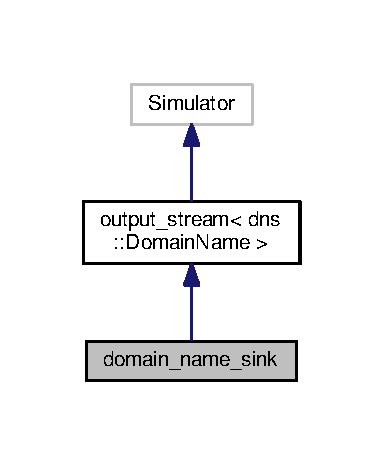
\includegraphics[width=184pt]{classdomain__name__sink__inherit__graph}
\end{center}
\end{figure}


Collaboration diagram for domain\+\_\+name\+\_\+sink\+:
\nopagebreak
\begin{figure}[H]
\begin{center}
\leavevmode
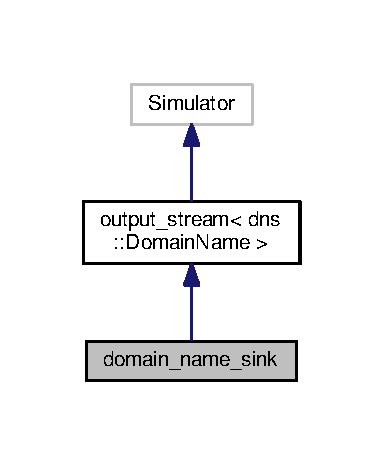
\includegraphics[width=184pt]{classdomain__name__sink__coll__graph}
\end{center}
\end{figure}
\subsection*{Public Member Functions}
\begin{DoxyCompactItemize}
\item 
{\bfseries domain\+\_\+name\+\_\+sink} (const char $\ast$n)\hypertarget{classdomain__name__sink_a3e4a6071da63647e596cbe5b855d386d}{}\label{classdomain__name__sink_a3e4a6071da63647e596cbe5b855d386d}

\end{DoxyCompactItemize}


The documentation for this class was generated from the following file\+:\begin{DoxyCompactItemize}
\item 
/home/lao/powerdevs/atomics/\+Network\+D\+E\+V\+S/domain\+\_\+name\+\_\+sink.\+h\end{DoxyCompactItemize}

\hypertarget{classdomain__name__source}{}\section{domain\+\_\+name\+\_\+source Class Reference}
\label{classdomain__name__source}\index{domain\+\_\+name\+\_\+source@{domain\+\_\+name\+\_\+source}}


A specialization of \hyperlink{classinput__stream}{input\+\_\+stream} template model to generate input of type \hyperlink{structdns_1_1DomainName}{dns\+::\+Domain\+Name} from a file.  




{\ttfamily \#include $<$domain\+\_\+name\+\_\+source.\+h$>$}



Inheritance diagram for domain\+\_\+name\+\_\+source\+:\nopagebreak
\begin{figure}[H]
\begin{center}
\leavevmode
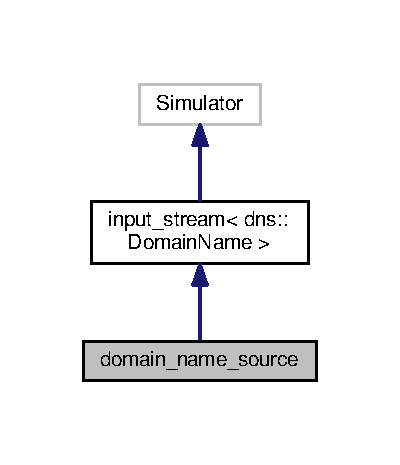
\includegraphics[width=192pt]{classdomain__name__source__inherit__graph}
\end{center}
\end{figure}


Collaboration diagram for domain\+\_\+name\+\_\+source\+:\nopagebreak
\begin{figure}[H]
\begin{center}
\leavevmode
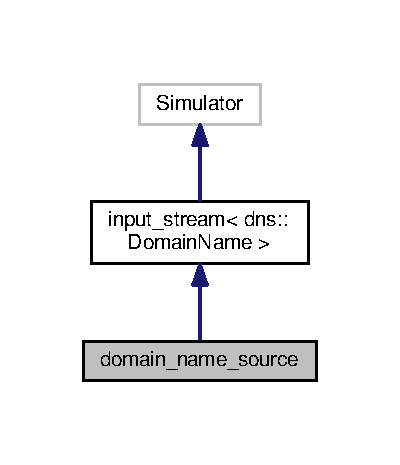
\includegraphics[width=192pt]{classdomain__name__source__coll__graph}
\end{center}
\end{figure}
\subsection*{Public Member Functions}
\begin{DoxyCompactItemize}
\item 
{\bfseries domain\+\_\+name\+\_\+source} (const char $\ast$n)\hypertarget{classdomain__name__source_a76cb055b27491617cad5842617bfe299}{}\label{classdomain__name__source_a76cb055b27491617cad5842617bfe299}

\end{DoxyCompactItemize}


\subsection{Detailed Description}
A specialization of \hyperlink{classinput__stream}{input\+\_\+stream} template model to generate input of type \hyperlink{structdns_1_1DomainName}{dns\+::\+Domain\+Name} from a file. 

\begin{DoxyAuthor}{Author}
Lauen Louan Mayal Belloli 
\end{DoxyAuthor}
\begin{DoxyDate}{Date}
14 May 2017 
\end{DoxyDate}


The documentation for this class was generated from the following file\+:\begin{DoxyCompactItemize}
\item 
/home/lao/powerdevs/atomics/\+Network\+D\+E\+V\+S/domain\+\_\+name\+\_\+source.\+h\end{DoxyCompactItemize}

\hypertarget{structdns_1_1DomainName}{}\section{dns\+:\+:Domain\+Name Struct Reference}
\label{structdns_1_1DomainName}\index{dns\+::\+Domain\+Name@{dns\+::\+Domain\+Name}}


This struct handles domain names with the format \textquotesingle{}zone1.\+zone2.\+zone3...zoneN\textquotesingle{}.  




{\ttfamily \#include $<$dns.\+h$>$}



Collaboration diagram for dns\+:\+:Domain\+Name\+:\nopagebreak
\begin{figure}[H]
\begin{center}
\leavevmode
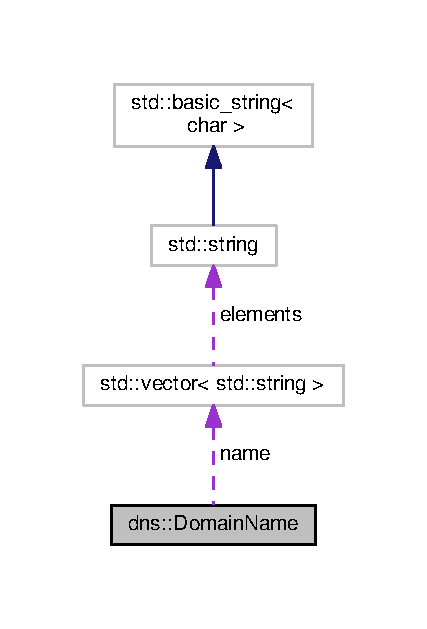
\includegraphics[width=205pt]{structdns_1_1DomainName__coll__graph}
\end{center}
\end{figure}
\subsection*{Public Member Functions}
\begin{DoxyCompactItemize}
\item 
\hyperlink{structdns_1_1DomainName_aa6753a696606acc35cb7df58ae22ca8d}{Domain\+Name} ()
\begin{DoxyCompactList}\small\item\em Default constructor. \end{DoxyCompactList}\item 
\hyperlink{structdns_1_1DomainName_ad60b6906c878a459d90e581e38a14b88}{Domain\+Name} (const \hyperlink{structdns_1_1DomainName}{Domain\+Name} \&other)
\begin{DoxyCompactList}\small\item\em Copy constructor. \end{DoxyCompactList}\item 
\hyperlink{structdns_1_1DomainName_ae5672debce76216a4fdc132d2f793f7d}{Domain\+Name} (std\+::string str)
\begin{DoxyCompactList}\small\item\em Constructor from std\+::string. \end{DoxyCompactList}\item 
\hyperlink{structdns_1_1DomainName_ae4dfa596bfe1f9a2ee9aa7d6a08a1288}{Domain\+Name} (const char $\ast$data)
\begin{DoxyCompactList}\small\item\em Constructor from const char $\ast$. \end{DoxyCompactList}\item 
const char $\ast$ \hyperlink{structdns_1_1DomainName_ae02a0ca9015d761bbea80711d18f4bf6}{c\+\_\+str} () const 
\item 
std\+::string \hyperlink{structdns_1_1DomainName_a139b1cb39d27b693f7662698e865536d}{as\+\_\+string} () const 
\begin{DoxyCompactList}\small\item\em Return the value of the instance in a std\+::string with the I\+DN format as required by the constructor from std\+::string. \end{DoxyCompactList}\item 
int \hyperlink{structdns_1_1DomainName_a894ccfcd88ac1ad2425b2bfe9ce826a6}{size} () const 
\item 
bool \hyperlink{structdns_1_1DomainName_a3c69c68df68eff0fa0f5009958119ba6}{operator==} (const \hyperlink{structdns_1_1DomainName}{Domain\+Name} \&other) const 
\begin{DoxyCompactList}\small\item\em Operator == for \hyperlink{structdns_1_1DomainName}{dns\+::\+Domain\+Name}. \end{DoxyCompactList}\end{DoxyCompactItemize}
\subsection*{Public Attributes}
\begin{DoxyCompactItemize}
\item 
std\+::vector$<$ std\+::string $>$ {\bfseries name}\hypertarget{structdns_1_1DomainName_a36d2107b7c6e3c78eb233244d22102ca}{}\label{structdns_1_1DomainName_a36d2107b7c6e3c78eb233244d22102ca}

\end{DoxyCompactItemize}


\subsection{Detailed Description}
This struct handles domain names with the format \textquotesingle{}zone1.\+zone2.\+zone3...zoneN\textquotesingle{}. 

\begin{DoxyAuthor}{Author}
Laouen Louan Mayal Belloli 
\end{DoxyAuthor}
\begin{DoxyDate}{Date}
14 May 2017
\end{DoxyDate}
This method allows to parse domain names from strings. An example of a \hyperlink{structdns_1_1DomainName}{dns\+::\+Domain\+Name} is \textquotesingle{}networks.\+devs.\+com\textquotesingle{} where \textquotesingle{}networks\textquotesingle{} es zone1 \textquotesingle{}devs\textquotesingle{} is zone2 and \textquotesingle{}com\textquotesingle{} is zone3. 

\subsection{Constructor \& Destructor Documentation}
\index{dns\+::\+Domain\+Name@{dns\+::\+Domain\+Name}!Domain\+Name@{Domain\+Name}}
\index{Domain\+Name@{Domain\+Name}!dns\+::\+Domain\+Name@{dns\+::\+Domain\+Name}}
\subsubsection[{\texorpdfstring{Domain\+Name()}{DomainName()}}]{\setlength{\rightskip}{0pt plus 5cm}dns\+::\+Domain\+Name\+::\+Domain\+Name (
\begin{DoxyParamCaption}
{}
\end{DoxyParamCaption}
)\hspace{0.3cm}{\ttfamily [inline]}}\hypertarget{structdns_1_1DomainName_aa6753a696606acc35cb7df58ae22ca8d}{}\label{structdns_1_1DomainName_aa6753a696606acc35cb7df58ae22ca8d}


Default constructor. 

Construct a new instance with an empty vale \textquotesingle{}\textquotesingle{} \index{dns\+::\+Domain\+Name@{dns\+::\+Domain\+Name}!Domain\+Name@{Domain\+Name}}
\index{Domain\+Name@{Domain\+Name}!dns\+::\+Domain\+Name@{dns\+::\+Domain\+Name}}
\subsubsection[{\texorpdfstring{Domain\+Name(const Domain\+Name \&other)}{DomainName(const DomainName &other)}}]{\setlength{\rightskip}{0pt plus 5cm}dns\+::\+Domain\+Name\+::\+Domain\+Name (
\begin{DoxyParamCaption}
\item[{const {\bf Domain\+Name} \&}]{other}
\end{DoxyParamCaption}
)\hspace{0.3cm}{\ttfamily [inline]}}\hypertarget{structdns_1_1DomainName_ad60b6906c878a459d90e581e38a14b88}{}\label{structdns_1_1DomainName_ad60b6906c878a459d90e581e38a14b88}


Copy constructor. 


\begin{DoxyParams}{Parameters}
{\em other} & A \hyperlink{structdns_1_1DomainName}{dns\+::\+Domain\+Name} to copy its value to construct the new instance. \\
\hline
\end{DoxyParams}
\index{dns\+::\+Domain\+Name@{dns\+::\+Domain\+Name}!Domain\+Name@{Domain\+Name}}
\index{Domain\+Name@{Domain\+Name}!dns\+::\+Domain\+Name@{dns\+::\+Domain\+Name}}
\subsubsection[{\texorpdfstring{Domain\+Name(std\+::string str)}{DomainName(std::string str)}}]{\setlength{\rightskip}{0pt plus 5cm}dns\+::\+Domain\+Name\+::\+Domain\+Name (
\begin{DoxyParamCaption}
\item[{std\+::string}]{str}
\end{DoxyParamCaption}
)\hspace{0.3cm}{\ttfamily [inline]}}\hypertarget{structdns_1_1DomainName_ae5672debce76216a4fdc132d2f793f7d}{}\label{structdns_1_1DomainName_ae5672debce76216a4fdc132d2f793f7d}


Constructor from std\+::string. 

This constructor uses a std\+::string formated in the I\+DN format.


\begin{DoxyParams}{Parameters}
{\em str} & A std\+::string used to construct the new instance. \\
\hline
\end{DoxyParams}
\index{dns\+::\+Domain\+Name@{dns\+::\+Domain\+Name}!Domain\+Name@{Domain\+Name}}
\index{Domain\+Name@{Domain\+Name}!dns\+::\+Domain\+Name@{dns\+::\+Domain\+Name}}
\subsubsection[{\texorpdfstring{Domain\+Name(const char $\ast$data)}{DomainName(const char *data)}}]{\setlength{\rightskip}{0pt plus 5cm}dns\+::\+Domain\+Name\+::\+Domain\+Name (
\begin{DoxyParamCaption}
\item[{const char $\ast$}]{data}
\end{DoxyParamCaption}
)\hspace{0.3cm}{\ttfamily [inline]}}\hypertarget{structdns_1_1DomainName_ae4dfa596bfe1f9a2ee9aa7d6a08a1288}{}\label{structdns_1_1DomainName_ae4dfa596bfe1f9a2ee9aa7d6a08a1288}


Constructor from const char $\ast$. 

This constructor uses a char $\ast$ representation to initialize the new instance. the format must be the next\+:

0xlen1zone10xlen2zone20xlen3...0xlen\+Nzone\+N0x00 where there is no space between the len and the zones name. The len are unsigned chars with the length in bytes of the zones names in text format and the len = 0x00 represent the end of the domain name.

example 0x08networks0x04devs0x03com0x00 = networks.\+devs.\+com


\begin{DoxyParams}{Parameters}
{\em data} & A const char $\ast$ used to inicialize the new instance \\
\hline
\end{DoxyParams}


\subsection{Member Function Documentation}
\index{dns\+::\+Domain\+Name@{dns\+::\+Domain\+Name}!as\+\_\+string@{as\+\_\+string}}
\index{as\+\_\+string@{as\+\_\+string}!dns\+::\+Domain\+Name@{dns\+::\+Domain\+Name}}
\subsubsection[{\texorpdfstring{as\+\_\+string() const }{as_string() const }}]{\setlength{\rightskip}{0pt plus 5cm}std\+::string dns\+::\+Domain\+Name\+::as\+\_\+string (
\begin{DoxyParamCaption}
{}
\end{DoxyParamCaption}
) const\hspace{0.3cm}{\ttfamily [inline]}}\hypertarget{structdns_1_1DomainName_a139b1cb39d27b693f7662698e865536d}{}\label{structdns_1_1DomainName_a139b1cb39d27b693f7662698e865536d}


Return the value of the instance in a std\+::string with the I\+DN format as required by the constructor from std\+::string. 

\begin{DoxyReturn}{Returns}
A std\+::string with the formated domain name value. 
\end{DoxyReturn}
\index{dns\+::\+Domain\+Name@{dns\+::\+Domain\+Name}!c\+\_\+str@{c\+\_\+str}}
\index{c\+\_\+str@{c\+\_\+str}!dns\+::\+Domain\+Name@{dns\+::\+Domain\+Name}}
\subsubsection[{\texorpdfstring{c\+\_\+str() const }{c_str() const }}]{\setlength{\rightskip}{0pt plus 5cm}const char$\ast$ dns\+::\+Domain\+Name\+::c\+\_\+str (
\begin{DoxyParamCaption}
{}
\end{DoxyParamCaption}
) const\hspace{0.3cm}{\ttfamily [inline]}}\hypertarget{structdns_1_1DomainName_ae02a0ca9015d761bbea80711d18f4bf6}{}\label{structdns_1_1DomainName_ae02a0ca9015d761bbea80711d18f4bf6}
\begin{DoxyReturn}{Returns}
A const char $\ast$ pointing to a memory block of a well defined representation as required by the constructor from const char $\ast$ of the instance domain name. 
\end{DoxyReturn}
\index{dns\+::\+Domain\+Name@{dns\+::\+Domain\+Name}!operator==@{operator==}}
\index{operator==@{operator==}!dns\+::\+Domain\+Name@{dns\+::\+Domain\+Name}}
\subsubsection[{\texorpdfstring{operator==(const Domain\+Name \&other) const }{operator==(const DomainName &other) const }}]{\setlength{\rightskip}{0pt plus 5cm}bool dns\+::\+Domain\+Name\+::operator== (
\begin{DoxyParamCaption}
\item[{const {\bf Domain\+Name} \&}]{other}
\end{DoxyParamCaption}
) const\hspace{0.3cm}{\ttfamily [inline]}}\hypertarget{structdns_1_1DomainName_a3c69c68df68eff0fa0f5009958119ba6}{}\label{structdns_1_1DomainName_a3c69c68df68eff0fa0f5009958119ba6}


Operator == for \hyperlink{structdns_1_1DomainName}{dns\+::\+Domain\+Name}. 

\begin{DoxyReturn}{Returns}
True if both the implicit this and the other instances are equals, False otherwise. 
\end{DoxyReturn}
\index{dns\+::\+Domain\+Name@{dns\+::\+Domain\+Name}!size@{size}}
\index{size@{size}!dns\+::\+Domain\+Name@{dns\+::\+Domain\+Name}}
\subsubsection[{\texorpdfstring{size() const }{size() const }}]{\setlength{\rightskip}{0pt plus 5cm}int dns\+::\+Domain\+Name\+::size (
\begin{DoxyParamCaption}
{}
\end{DoxyParamCaption}
) const\hspace{0.3cm}{\ttfamily [inline]}}\hypertarget{structdns_1_1DomainName_a894ccfcd88ac1ad2425b2bfe9ce826a6}{}\label{structdns_1_1DomainName_a894ccfcd88ac1ad2425b2bfe9ce826a6}
\begin{DoxyReturn}{Returns}
A int with the zise of the current domain name with is the sum of the size in bytes of all the zones of the domain. 
\end{DoxyReturn}


The documentation for this struct was generated from the following file\+:\begin{DoxyCompactItemize}
\item 
/home/lao/\+Documents/git/\+Network\+D\+E\+V\+S/structures/dns.\+h\end{DoxyCompactItemize}

\hypertarget{structlink_1_1arp_1_1Entry}{}\section{link\+:\+:arp\+:\+:Entry Struct Reference}
\label{structlink_1_1arp_1_1Entry}\index{link\+::arp\+::\+Entry@{link\+::arp\+::\+Entry}}


This struct represent an entry in the A\+RP cache Table.  




{\ttfamily \#include $<$link.\+h$>$}



Collaboration diagram for link\+:\+:arp\+:\+:Entry\+:\nopagebreak
\begin{figure}[H]
\begin{center}
\leavevmode
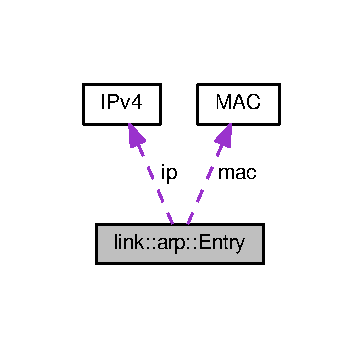
\includegraphics[width=174pt]{structlink_1_1arp_1_1Entry__coll__graph}
\end{center}
\end{figure}
\subsection*{Public Member Functions}
\begin{DoxyCompactItemize}
\item 
\hyperlink{structlink_1_1arp_1_1Entry_af14702ffc3a1b10e45a148220af6b5d4}{Entry} ()
\begin{DoxyCompactList}\small\item\em Default constructor. \end{DoxyCompactList}\item 
\hyperlink{structlink_1_1arp_1_1Entry_ab2adef8c42d08549d72c9fba0839da5c}{Entry} (const \hyperlink{structlink_1_1arp_1_1Entry}{Entry} \&other)
\begin{DoxyCompactList}\small\item\em Copy instance. \end{DoxyCompactList}\end{DoxyCompactItemize}
\subsection*{Public Attributes}
\begin{DoxyCompactItemize}
\item 
\hyperlink{structIPv4}{I\+Pv4} {\bfseries ip}\hypertarget{structlink_1_1arp_1_1Entry_a40929f76ac846faefab32e92b290c92f}{}\label{structlink_1_1arp_1_1Entry_a40929f76ac846faefab32e92b290c92f}

\item 
\hyperlink{structMAC}{M\+AC} {\bfseries mac}\hypertarget{structlink_1_1arp_1_1Entry_a72cdde0b5131b1ecc350f5ae28bb7f8a}{}\label{structlink_1_1arp_1_1Entry_a72cdde0b5131b1ecc350f5ae28bb7f8a}

\item 
double {\bfseries timeout}\hypertarget{structlink_1_1arp_1_1Entry_a8838c1d16cd38f16032703d00742df7a}{}\label{structlink_1_1arp_1_1Entry_a8838c1d16cd38f16032703d00742df7a}

\end{DoxyCompactItemize}


\subsection{Detailed Description}
This struct represent an entry in the A\+RP cache Table. 

\begin{DoxyAuthor}{Author}
Laouen Louan Mayal Belloli 
\end{DoxyAuthor}
\begin{DoxyDate}{Date}
14 May 2017
\end{DoxyDate}
A \hyperlink{structlink_1_1arp_1_1Entry}{link\+::arp\+::\+Entry} has the next fields\+:
\begin{DoxyEnumerate}
\item ip\+: The \hyperlink{structIPv4}{I\+Pv4} to get the \hyperlink{structMAC}{M\+AC} Address.
\item mac\+: The already obtained \hyperlink{structMAC}{M\+AC} address of ip.
\item timeout\+: The cache timeout in seconds before remove the entry from the A\+RP cache table. 
\end{DoxyEnumerate}

\subsection{Constructor \& Destructor Documentation}
\index{link\+::arp\+::\+Entry@{link\+::arp\+::\+Entry}!Entry@{Entry}}
\index{Entry@{Entry}!link\+::arp\+::\+Entry@{link\+::arp\+::\+Entry}}
\subsubsection[{\texorpdfstring{Entry()}{Entry()}}]{\setlength{\rightskip}{0pt plus 5cm}link\+::arp\+::\+Entry\+::\+Entry (
\begin{DoxyParamCaption}
{}
\end{DoxyParamCaption}
)\hspace{0.3cm}{\ttfamily [inline]}}\hypertarget{structlink_1_1arp_1_1Entry_af14702ffc3a1b10e45a148220af6b5d4}{}\label{structlink_1_1arp_1_1Entry_af14702ffc3a1b10e45a148220af6b5d4}


Default constructor. 

Construct a new empty instance. \index{link\+::arp\+::\+Entry@{link\+::arp\+::\+Entry}!Entry@{Entry}}
\index{Entry@{Entry}!link\+::arp\+::\+Entry@{link\+::arp\+::\+Entry}}
\subsubsection[{\texorpdfstring{Entry(const Entry \&other)}{Entry(const Entry &other)}}]{\setlength{\rightskip}{0pt plus 5cm}link\+::arp\+::\+Entry\+::\+Entry (
\begin{DoxyParamCaption}
\item[{const {\bf Entry} \&}]{other}
\end{DoxyParamCaption}
)\hspace{0.3cm}{\ttfamily [inline]}}\hypertarget{structlink_1_1arp_1_1Entry_ab2adef8c42d08549d72c9fba0839da5c}{}\label{structlink_1_1arp_1_1Entry_ab2adef8c42d08549d72c9fba0839da5c}


Copy instance. 

Construct a new copy of the instances passed as parameter.


\begin{DoxyParams}{Parameters}
{\em other} & The \hyperlink{structlink_1_1arp_1_1Entry}{link\+::arp\+::\+Entry} to copy in the new instance. \\
\hline
\end{DoxyParams}


The documentation for this struct was generated from the following file\+:\begin{DoxyCompactItemize}
\item 
/home/lao/\+Documents/git/\+Network\+D\+E\+V\+S/structures/link.\+h\end{DoxyCompactItemize}

\hypertarget{structip_1_1Forwarding__entry}{}\section{ip\+:\+:Forwarding\+\_\+entry Struct Reference}
\label{structip_1_1Forwarding__entry}\index{ip\+::\+Forwarding\+\_\+entry@{ip\+::\+Forwarding\+\_\+entry}}


Represent an entry of the forwarding table of the ip protocol.  




{\ttfamily \#include $<$ip.\+h$>$}



Collaboration diagram for ip\+:\+:Forwarding\+\_\+entry\+:\nopagebreak
\begin{figure}[H]
\begin{center}
\leavevmode
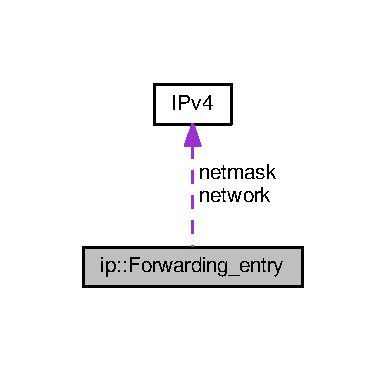
\includegraphics[width=185pt]{structip_1_1Forwarding__entry__coll__graph}
\end{center}
\end{figure}
\subsection*{Public Member Functions}
\begin{DoxyCompactItemize}
\item 
\hyperlink{structip_1_1Forwarding__entry_af4c7f746d7de8206146adf933ad3dbe8}{Forwarding\+\_\+entry} ()
\begin{DoxyCompactList}\small\item\em Default constructor. \end{DoxyCompactList}\item 
\hyperlink{structip_1_1Forwarding__entry_a9cdd6c01091d718a32a11342c3998f9f}{Forwarding\+\_\+entry} (const \hyperlink{structip_1_1Forwarding__entry}{Forwarding\+\_\+entry} \&other)
\begin{DoxyCompactList}\small\item\em Copy constructor. \end{DoxyCompactList}\item 
bool \hyperlink{structip_1_1Forwarding__entry_a15177e8af63ffd9d41a72a55abfcbb58}{same\+Subnet} (\hyperlink{structIPv4}{I\+Pv4} des\+\_\+ip) const 
\begin{DoxyCompactList}\small\item\em Cheks whether the other remote host is in the implicit this-\/$>$network or not. \end{DoxyCompactList}\item 
std\+::string \hyperlink{structip_1_1Forwarding__entry_a7b005eaf733338c728b9e63c00a84668}{as\+\_\+string} () const 
\begin{DoxyCompactList}\small\item\em Prints in a std\+::string a human redable version of the ip\+::\+Forwarding\+\_\+table. \end{DoxyCompactList}\end{DoxyCompactItemize}
\subsection*{Public Attributes}
\begin{DoxyCompactItemize}
\item 
\hyperlink{structIPv4}{I\+Pv4} {\bfseries network}\hypertarget{structip_1_1Forwarding__entry_aec0c736499656bd68f001cc50b6b4017}{}\label{structip_1_1Forwarding__entry_aec0c736499656bd68f001cc50b6b4017}

\item 
\hyperlink{structIPv4}{I\+Pv4} {\bfseries netmask}\hypertarget{structip_1_1Forwarding__entry_a51b8230ced4d6e7ea1e17f357bea242a}{}\label{structip_1_1Forwarding__entry_a51b8230ced4d6e7ea1e17f357bea242a}

\item 
ushort {\bfseries interface}\hypertarget{structip_1_1Forwarding__entry_aa84edda440aa39d70142b02320be2e07}{}\label{structip_1_1Forwarding__entry_aa84edda440aa39d70142b02320be2e07}

\end{DoxyCompactItemize}


\subsection{Detailed Description}
Represent an entry of the forwarding table of the ip protocol. 

\begin{DoxyAuthor}{Author}
Laouen Louan Mayal Belloli 
\end{DoxyAuthor}
\begin{DoxyDate}{Date}
14 May 2017
\end{DoxyDate}
The \hyperlink{structip_1_1Forwarding__entry}{ip\+::\+Forwarding\+\_\+entry} has the next field\+:
\begin{DoxyEnumerate}
\item network\+: a \hyperlink{structIPv4}{I\+Pv4} containing the subnet of the next hope.
\item netmask\+: a \hyperlink{structIPv4}{I\+Pv4} containing the mask that indicate what bits of the network represent the network of the next hope.
\item interface\+: an unsigned short with the interface where to send the \hyperlink{structip_1_1Datagram}{ip\+::\+Datagram} to reach the next hope. 
\end{DoxyEnumerate}

\subsection{Constructor \& Destructor Documentation}
\index{ip\+::\+Forwarding\+\_\+entry@{ip\+::\+Forwarding\+\_\+entry}!Forwarding\+\_\+entry@{Forwarding\+\_\+entry}}
\index{Forwarding\+\_\+entry@{Forwarding\+\_\+entry}!ip\+::\+Forwarding\+\_\+entry@{ip\+::\+Forwarding\+\_\+entry}}
\subsubsection[{\texorpdfstring{Forwarding\+\_\+entry()}{Forwarding_entry()}}]{\setlength{\rightskip}{0pt plus 5cm}ip\+::\+Forwarding\+\_\+entry\+::\+Forwarding\+\_\+entry (
\begin{DoxyParamCaption}
{}
\end{DoxyParamCaption}
)\hspace{0.3cm}{\ttfamily [inline]}}\hypertarget{structip_1_1Forwarding__entry_af4c7f746d7de8206146adf933ad3dbe8}{}\label{structip_1_1Forwarding__entry_af4c7f746d7de8206146adf933ad3dbe8}


Default constructor. 

Construct a new empty instance. \index{ip\+::\+Forwarding\+\_\+entry@{ip\+::\+Forwarding\+\_\+entry}!Forwarding\+\_\+entry@{Forwarding\+\_\+entry}}
\index{Forwarding\+\_\+entry@{Forwarding\+\_\+entry}!ip\+::\+Forwarding\+\_\+entry@{ip\+::\+Forwarding\+\_\+entry}}
\subsubsection[{\texorpdfstring{Forwarding\+\_\+entry(const Forwarding\+\_\+entry \&other)}{Forwarding_entry(const Forwarding_entry &other)}}]{\setlength{\rightskip}{0pt plus 5cm}ip\+::\+Forwarding\+\_\+entry\+::\+Forwarding\+\_\+entry (
\begin{DoxyParamCaption}
\item[{const {\bf Forwarding\+\_\+entry} \&}]{other}
\end{DoxyParamCaption}
)\hspace{0.3cm}{\ttfamily [inline]}}\hypertarget{structip_1_1Forwarding__entry_a9cdd6c01091d718a32a11342c3998f9f}{}\label{structip_1_1Forwarding__entry_a9cdd6c01091d718a32a11342c3998f9f}


Copy constructor. 

Construct a new instance with a copy of the one passed as parameter.


\begin{DoxyParams}{Parameters}
{\em other} & The \hyperlink{structip_1_1Forwarding__entry}{ip\+::\+Forwarding\+\_\+entry} used to construct the new copy. \\
\hline
\end{DoxyParams}


\subsection{Member Function Documentation}
\index{ip\+::\+Forwarding\+\_\+entry@{ip\+::\+Forwarding\+\_\+entry}!as\+\_\+string@{as\+\_\+string}}
\index{as\+\_\+string@{as\+\_\+string}!ip\+::\+Forwarding\+\_\+entry@{ip\+::\+Forwarding\+\_\+entry}}
\subsubsection[{\texorpdfstring{as\+\_\+string() const }{as_string() const }}]{\setlength{\rightskip}{0pt plus 5cm}std\+::string ip\+::\+Forwarding\+\_\+entry\+::as\+\_\+string (
\begin{DoxyParamCaption}
{}
\end{DoxyParamCaption}
) const\hspace{0.3cm}{\ttfamily [inline]}}\hypertarget{structip_1_1Forwarding__entry_a7b005eaf733338c728b9e63c00a84668}{}\label{structip_1_1Forwarding__entry_a7b005eaf733338c728b9e63c00a84668}


Prints in a std\+::string a human redable version of the ip\+::\+Forwarding\+\_\+table. 

\begin{DoxyReturn}{Returns}
A std\+::string with the value printed on it. 
\end{DoxyReturn}
\index{ip\+::\+Forwarding\+\_\+entry@{ip\+::\+Forwarding\+\_\+entry}!same\+Subnet@{same\+Subnet}}
\index{same\+Subnet@{same\+Subnet}!ip\+::\+Forwarding\+\_\+entry@{ip\+::\+Forwarding\+\_\+entry}}
\subsubsection[{\texorpdfstring{same\+Subnet(\+I\+Pv4 des\+\_\+ip) const }{sameSubnet(IPv4 des_ip) const }}]{\setlength{\rightskip}{0pt plus 5cm}bool ip\+::\+Forwarding\+\_\+entry\+::same\+Subnet (
\begin{DoxyParamCaption}
\item[{{\bf I\+Pv4}}]{des\+\_\+ip}
\end{DoxyParamCaption}
) const\hspace{0.3cm}{\ttfamily [inline]}}\hypertarget{structip_1_1Forwarding__entry_a15177e8af63ffd9d41a72a55abfcbb58}{}\label{structip_1_1Forwarding__entry_a15177e8af63ffd9d41a72a55abfcbb58}


Cheks whether the other remote host is in the implicit this-\/$>$network or not. 


\begin{DoxyParams}{Parameters}
{\em des\+\_\+ip} & The \hyperlink{structIPv4}{I\+Pv4} of the remote host to check if is in the same subnet. \\
\hline
\end{DoxyParams}
\begin{DoxyReturn}{Returns}
True if des\+\_\+ip is in the same subnate of this-\/$>$network. 
\end{DoxyReturn}


The documentation for this struct was generated from the following file\+:\begin{DoxyCompactItemize}
\item 
/home/lao/\+Documents/git/\+Network\+D\+E\+V\+S/structures/ip.\+h\end{DoxyCompactItemize}

\hypertarget{structsw_1_1Forwarding__entry}{}\section{sw\+:\+:Forwarding\+\_\+entry Struct Reference}
\label{structsw_1_1Forwarding__entry}\index{sw\+::\+Forwarding\+\_\+entry@{sw\+::\+Forwarding\+\_\+entry}}


Collaboration diagram for sw\+:\+:Forwarding\+\_\+entry\+:\nopagebreak
\begin{figure}[H]
\begin{center}
\leavevmode
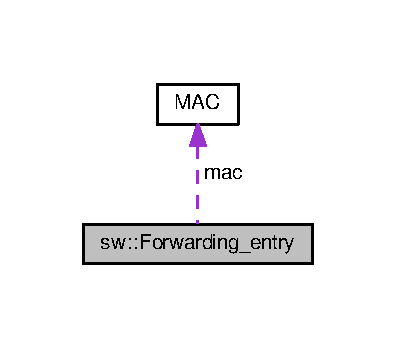
\includegraphics[width=190pt]{structsw_1_1Forwarding__entry__coll__graph}
\end{center}
\end{figure}
\subsection*{Public Member Functions}
\begin{DoxyCompactItemize}
\item 
{\bfseries Forwarding\+\_\+entry} (const \hyperlink{structsw_1_1Forwarding__entry}{Forwarding\+\_\+entry} \&other)\hypertarget{structsw_1_1Forwarding__entry_a504b52199970b085a23a28cd45b9b788}{}\label{structsw_1_1Forwarding__entry_a504b52199970b085a23a28cd45b9b788}

\end{DoxyCompactItemize}
\subsection*{Public Attributes}
\begin{DoxyCompactItemize}
\item 
\hyperlink{structMAC}{M\+AC} {\bfseries mac}\hypertarget{structsw_1_1Forwarding__entry_a69db303ecdfc75db66ea09b459ace6fc}{}\label{structsw_1_1Forwarding__entry_a69db303ecdfc75db66ea09b459ace6fc}

\item 
ushort {\bfseries interface}\hypertarget{structsw_1_1Forwarding__entry_ab08b8f0d50af0a13308f5fc5224586d6}{}\label{structsw_1_1Forwarding__entry_ab08b8f0d50af0a13308f5fc5224586d6}

\end{DoxyCompactItemize}


The documentation for this struct was generated from the following file\+:\begin{DoxyCompactItemize}
\item 
/home/lao/powerdevs/atomics/\+Network\+D\+E\+V\+S/structures/sw.\+h\end{DoxyCompactItemize}

\hypertarget{structlink_1_1Frame}{}\section{link\+:\+:Frame Struct Reference}
\label{structlink_1_1Frame}\index{link\+::\+Frame@{link\+::\+Frame}}


Implement a L2 frame.  




{\ttfamily \#include $<$link.\+h$>$}



Inheritance diagram for link\+:\+:Frame\+:\nopagebreak
\begin{figure}[H]
\begin{center}
\leavevmode
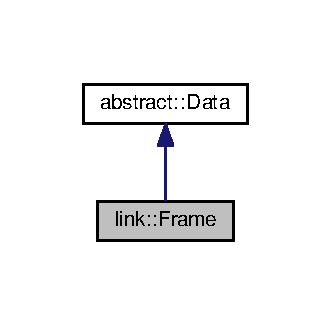
\includegraphics[width=159pt]{structlink_1_1Frame__inherit__graph}
\end{center}
\end{figure}


Collaboration diagram for link\+:\+:Frame\+:\nopagebreak
\begin{figure}[H]
\begin{center}
\leavevmode
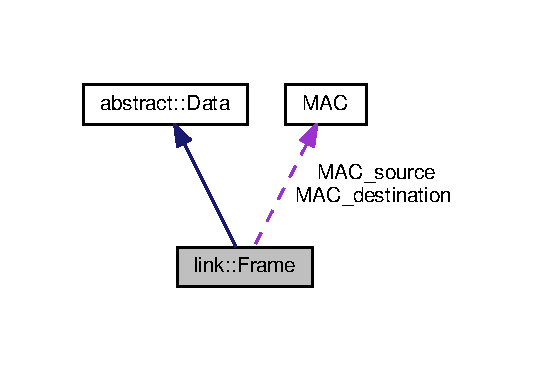
\includegraphics[width=258pt]{structlink_1_1Frame__coll__graph}
\end{center}
\end{figure}
\subsection*{Public Member Functions}
\begin{DoxyCompactItemize}
\item 
\hyperlink{structlink_1_1Frame_a66cdf70363bbb87ff48c661fdeb63242}{Frame} ()
\begin{DoxyCompactList}\small\item\em Default constructor. \end{DoxyCompactList}\item 
\hyperlink{structlink_1_1Frame_aea0b6d8d213840254aac152351a7c46a}{Frame} (const \hyperlink{structlink_1_1Frame}{Frame} \&other)
\begin{DoxyCompactList}\small\item\em Copy constructor. \end{DoxyCompactList}\item 
void \hyperlink{structlink_1_1Frame_a7dfe0d1f9213795013c55120438b9790}{disable\+A\+R\+P\+Flag} ()\hypertarget{structlink_1_1Frame_a7dfe0d1f9213795013c55120438b9790}{}\label{structlink_1_1Frame_a7dfe0d1f9213795013c55120438b9790}

\begin{DoxyCompactList}\small\item\em It set the preamble A\+RP flag as desabled to tell that the L2 frame carries an \hyperlink{structip_1_1Datagram}{ip\+::\+Datagram}. \end{DoxyCompactList}\item 
void \hyperlink{structlink_1_1Frame_aa27284375795ced3f503efcd617fb65e}{enable\+A\+R\+P\+Flag} ()
\begin{DoxyCompactList}\small\item\em It set the preamble A\+RP flag as enables to tell that the L2 frame carries an A\+RP Packet. \end{DoxyCompactList}\item 
void \hyperlink{structlink_1_1Frame_af14b9acc0bd67497f8d008425c36462e}{set\+Payload} (const \hyperlink{structip_1_1Datagram}{ip\+::\+Datagram} \&p)\hypertarget{structlink_1_1Frame_af14b9acc0bd67497f8d008425c36462e}{}\label{structlink_1_1Frame_af14b9acc0bd67497f8d008425c36462e}

\begin{DoxyCompactList}\small\item\em Sets an \hyperlink{structip_1_1Datagram}{ip\+::\+Datagram} as the payload and desables the A\+RP flags. \end{DoxyCompactList}\item 
void \hyperlink{structlink_1_1Frame_a9eb67e1eb8d928dba0a42451edb590eb}{set\+Payload} (const \hyperlink{structlink_1_1arp_1_1Packet}{arp\+::\+Packet} \&p)\hypertarget{structlink_1_1Frame_a9eb67e1eb8d928dba0a42451edb590eb}{}\label{structlink_1_1Frame_a9eb67e1eb8d928dba0a42451edb590eb}

\begin{DoxyCompactList}\small\item\em Sets a \hyperlink{structlink_1_1arp_1_1Packet}{link\+::arp\+::\+Packet} as the payload and enables the A\+RP flags. \end{DoxyCompactList}\end{DoxyCompactItemize}
\subsection*{Public Attributes}
\begin{DoxyCompactItemize}
\item 
unsigned long {\bfseries preamble}\hypertarget{structlink_1_1Frame_a560843e736beacb7e8dec851f4ee1f9e}{}\label{structlink_1_1Frame_a560843e736beacb7e8dec851f4ee1f9e}

\item 
\hyperlink{structMAC}{M\+AC} {\bfseries M\+A\+C\+\_\+destination}\hypertarget{structlink_1_1Frame_aa85e5728d6dfab309546d55c74a5def3}{}\label{structlink_1_1Frame_aa85e5728d6dfab309546d55c74a5def3}

\item 
\hyperlink{structMAC}{M\+AC} {\bfseries M\+A\+C\+\_\+source}\hypertarget{structlink_1_1Frame_a972ec99e9747b045143f6d7c6f4e0bd3}{}\label{structlink_1_1Frame_a972ec99e9747b045143f6d7c6f4e0bd3}

\item 
ushort {\bfseries Ether\+Type}\hypertarget{structlink_1_1Frame_a6ae867ac5cf3d8949d0a8ed72683e14d}{}\label{structlink_1_1Frame_a6ae867ac5cf3d8949d0a8ed72683e14d}

\item 
char {\bfseries payload} \mbox{[}1500\mbox{]}\hypertarget{structlink_1_1Frame_a0aca61f4762da429483aff778ec9f01f}{}\label{structlink_1_1Frame_a0aca61f4762da429483aff778ec9f01f}

\item 
unsigned long {\bfseries C\+RC}\hypertarget{structlink_1_1Frame_abeaa6f98cfe999333b31926b6caf5d84}{}\label{structlink_1_1Frame_abeaa6f98cfe999333b31926b6caf5d84}

\item 
u\+\_\+char {\bfseries interpacket\+\_\+gat} \mbox{[}12\mbox{]}\hypertarget{structlink_1_1Frame_a949962d7ee45bbcf1787640c797e5bf8}{}\label{structlink_1_1Frame_a949962d7ee45bbcf1787640c797e5bf8}

\end{DoxyCompactItemize}


\subsection{Detailed Description}
Implement a L2 frame. 

\begin{DoxyAuthor}{Author}
Laouen Louan Mayal Belloli 
\end{DoxyAuthor}
\begin{DoxyDate}{Date}
14 May 2017
\end{DoxyDate}
A L2 \hyperlink{structlink_1_1Frame}{Frame} contains the next fields\+: preamble\+: an unsigned long with all the required flags. M\+A\+C\+\_\+destination\+: The \hyperlink{structMAC}{M\+AC} Address of the destination host. M\+A\+C\+\_\+source\+: The \hyperlink{structMAC}{M\+AC} Address of the source host. Ether\+Type\+: Type of the fisical protocol (0 for Ethernet). payload\+: a char\mbox{[}1500\mbox{]} with the \hyperlink{structip_1_1Datagram}{ip\+::\+Datagram} or A\+RP Paket to send. interpacket\+\_\+gat\+: a char\mbox{[}12\mbox{]} used to avoid solve some networks colitions problems. 

\subsection{Constructor \& Destructor Documentation}
\index{link\+::\+Frame@{link\+::\+Frame}!Frame@{Frame}}
\index{Frame@{Frame}!link\+::\+Frame@{link\+::\+Frame}}
\subsubsection[{\texorpdfstring{Frame()}{Frame()}}]{\setlength{\rightskip}{0pt plus 5cm}link\+::\+Frame\+::\+Frame (
\begin{DoxyParamCaption}
{}
\end{DoxyParamCaption}
)\hspace{0.3cm}{\ttfamily [inline]}}\hypertarget{structlink_1_1Frame_a66cdf70363bbb87ff48c661fdeb63242}{}\label{structlink_1_1Frame_a66cdf70363bbb87ff48c661fdeb63242}


Default constructor. 

Construct a new empty instance. \index{link\+::\+Frame@{link\+::\+Frame}!Frame@{Frame}}
\index{Frame@{Frame}!link\+::\+Frame@{link\+::\+Frame}}
\subsubsection[{\texorpdfstring{Frame(const Frame \&other)}{Frame(const Frame &other)}}]{\setlength{\rightskip}{0pt plus 5cm}link\+::\+Frame\+::\+Frame (
\begin{DoxyParamCaption}
\item[{const {\bf Frame} \&}]{other}
\end{DoxyParamCaption}
)\hspace{0.3cm}{\ttfamily [inline]}}\hypertarget{structlink_1_1Frame_aea0b6d8d213840254aac152351a7c46a}{}\label{structlink_1_1Frame_aea0b6d8d213840254aac152351a7c46a}


Copy constructor. 

Construct a copy of the instance passed as parameter.


\begin{DoxyParams}{Parameters}
{\em other} & The \hyperlink{structlink_1_1Frame}{link\+::\+Frame} to copy in the new instance. \\
\hline
\end{DoxyParams}


\subsection{Member Function Documentation}
\index{link\+::\+Frame@{link\+::\+Frame}!enable\+A\+R\+P\+Flag@{enable\+A\+R\+P\+Flag}}
\index{enable\+A\+R\+P\+Flag@{enable\+A\+R\+P\+Flag}!link\+::\+Frame@{link\+::\+Frame}}
\subsubsection[{\texorpdfstring{enable\+A\+R\+P\+Flag()}{enableARPFlag()}}]{\setlength{\rightskip}{0pt plus 5cm}void link\+::\+Frame\+::enable\+A\+R\+P\+Flag (
\begin{DoxyParamCaption}
{}
\end{DoxyParamCaption}
)\hspace{0.3cm}{\ttfamily [inline]}}\hypertarget{structlink_1_1Frame_aa27284375795ced3f503efcd617fb65e}{}\label{structlink_1_1Frame_aa27284375795ced3f503efcd617fb65e}


It set the preamble A\+RP flag as enables to tell that the L2 frame carries an A\+RP Packet. 

\mbox{[}long description\mbox{]} 

The documentation for this struct was generated from the following file\+:\begin{DoxyCompactItemize}
\item 
/home/lao/\+Documents/git/\+Network\+D\+E\+V\+S/structures/link.\+h\end{DoxyCompactItemize}

\hypertarget{structswp_1_1Hdr}{}\section{swp\+:\+:Hdr Struct Reference}
\label{structswp_1_1Hdr}\index{swp\+::\+Hdr@{swp\+::\+Hdr}}
\subsection*{Public Attributes}
\begin{DoxyCompactItemize}
\item 
Seqno {\bfseries Seq\+Num}\hypertarget{structswp_1_1Hdr_a2c4899f7de5ac69d97e0944abadfd80a}{}\label{structswp_1_1Hdr_a2c4899f7de5ac69d97e0944abadfd80a}

\item 
Seqno {\bfseries Ack\+Num}\hypertarget{structswp_1_1Hdr_a8f1b40013225b925c8e88d4486d24733}{}\label{structswp_1_1Hdr_a8f1b40013225b925c8e88d4486d24733}

\item 
u\+\_\+char {\bfseries Flags}\hypertarget{structswp_1_1Hdr_a7e60a051ee14be6f6eb1da4f8a01b7a9}{}\label{structswp_1_1Hdr_a7e60a051ee14be6f6eb1da4f8a01b7a9}

\end{DoxyCompactItemize}


The documentation for this struct was generated from the following file\+:\begin{DoxyCompactItemize}
\item 
/home/lao/powerdevs/atomics/\+Network\+D\+E\+V\+S/structures/swp.\+h\end{DoxyCompactItemize}

\hypertarget{structabstract_1_1Header}{}\section{abstract\+:\+:Header Struct Reference}
\label{structabstract_1_1Header}\index{abstract\+::\+Header@{abstract\+::\+Header}}


Inheritance diagram for abstract\+:\+:Header\+:\nopagebreak
\begin{figure}[H]
\begin{center}
\leavevmode
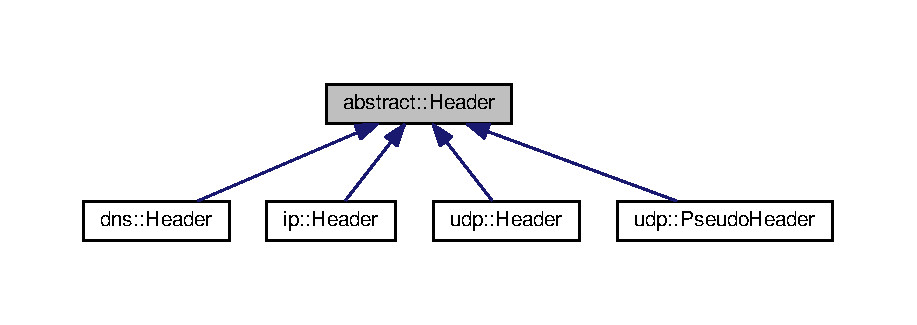
\includegraphics[width=350pt]{structabstract_1_1Header__inherit__graph}
\end{center}
\end{figure}


The documentation for this struct was generated from the following file\+:\begin{DoxyCompactItemize}
\item 
/home/lao/powerdevs/atomics/\+Network\+D\+E\+V\+S/structures/abstract\+\_\+types.\+h\end{DoxyCompactItemize}

\hypertarget{structdns_1_1Header}{}\section{dns\+:\+:Header Struct Reference}
\label{structdns_1_1Header}\index{dns\+::\+Header@{dns\+::\+Header}}


Structure that implements a \hyperlink{structdns_1_1Packet}{dns\+::\+Packet} header.  




{\ttfamily \#include $<$dns.\+h$>$}



Inheritance diagram for dns\+:\+:Header\+:\nopagebreak
\begin{figure}[H]
\begin{center}
\leavevmode
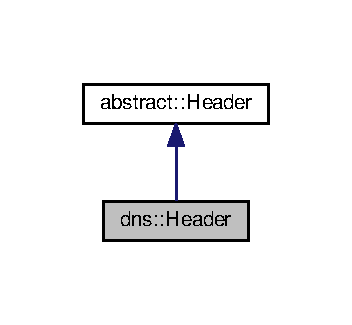
\includegraphics[width=169pt]{structdns_1_1Header__inherit__graph}
\end{center}
\end{figure}


Collaboration diagram for dns\+:\+:Header\+:\nopagebreak
\begin{figure}[H]
\begin{center}
\leavevmode
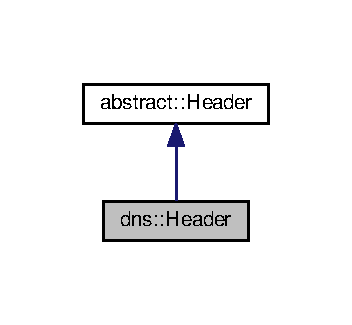
\includegraphics[width=169pt]{structdns_1_1Header__coll__graph}
\end{center}
\end{figure}
\subsection*{Public Member Functions}
\begin{DoxyCompactItemize}
\item 
\hyperlink{structdns_1_1Header_ab15c37ac6b02f5186082ea6a2f40edc0}{Header} ()
\begin{DoxyCompactList}\small\item\em Default constructor. \end{DoxyCompactList}\item 
\hyperlink{structdns_1_1Header_ab7d03fd2cec0659afe0df11f59a3b4da}{Header} (const \hyperlink{structdns_1_1Header}{Header} \&other)
\begin{DoxyCompactList}\small\item\em Copy contructor. \end{DoxyCompactList}\item 
\hyperlink{structdns_1_1Header_a5195a1241799e64eea7c5061f81a7c4e}{Header} (const char $\ast$const other)
\begin{DoxyCompactList}\small\item\em Contructor from const char$\ast$. \end{DoxyCompactList}\item 
void \hyperlink{structdns_1_1Header_ac8629bfb54bfe73b2a85ad3ab04e4561}{set\+Flag} (uint16\+\_\+t flag, uint16\+\_\+t mask)
\begin{DoxyCompactList}\small\item\em Uses the mask to set the correct bits of the flags\+\_\+code field of the instance with the value the bits in the flag parameter in those positions. \end{DoxyCompactList}\item 
bool \hyperlink{structdns_1_1Header_aee9ceec6332d282f329b967cef1d285c}{is} (uint16\+\_\+t flag, uint16\+\_\+t mask) const 
\begin{DoxyCompactList}\small\item\em Checks whether the flags\+\_\+code is set with the flag passed as parameter. \end{DoxyCompactList}\item 
ushort \hyperlink{structdns_1_1Header_abffe9b9ee5acba609e687535354ba6c8}{size} () const 
\item 
const char $\ast$ \hyperlink{structdns_1_1Header_a9b1a9610e54c5c0992fe6e756c8fadbb}{c\+\_\+str} () const 
\begin{DoxyCompactList}\small\item\em Copy all the bytes of the instance in a memory block and return a pointer to that memory block. \end{DoxyCompactList}\item 
std\+::string \hyperlink{structdns_1_1Header_a8f7e8d1e1e08f9b6734a83fafa4aca7f}{as\+\_\+string} () const 
\begin{DoxyCompactList}\small\item\em Returns a string formated with the \hyperlink{structdns_1_1Header}{dns\+::\+Header} value of the this. \end{DoxyCompactList}\end{DoxyCompactItemize}
\subsection*{Public Attributes}
\begin{DoxyCompactItemize}
\item 
ushort {\bfseries id}\hypertarget{structdns_1_1Header_a93db6477169afa0916eb97e18d0d414d}{}\label{structdns_1_1Header_a93db6477169afa0916eb97e18d0d414d}

\item 
ushort {\bfseries flags\+\_\+code}\hypertarget{structdns_1_1Header_afd9a0c9f79092a0baa8ad67d8f8cfcf5}{}\label{structdns_1_1Header_afd9a0c9f79092a0baa8ad67d8f8cfcf5}

\item 
ushort {\bfseries Q\+D\+Count}\hypertarget{structdns_1_1Header_ac4606baefe48fdda25fe00693426cac6}{}\label{structdns_1_1Header_ac4606baefe48fdda25fe00693426cac6}

\item 
ushort {\bfseries A\+N\+Count}\hypertarget{structdns_1_1Header_a47cd880532a4aaad40e32c2c2b10bf83}{}\label{structdns_1_1Header_a47cd880532a4aaad40e32c2c2b10bf83}

\item 
ushort {\bfseries N\+S\+Count}\hypertarget{structdns_1_1Header_ace802bcf38b0de507788d7fb5f4ca082}{}\label{structdns_1_1Header_ace802bcf38b0de507788d7fb5f4ca082}

\item 
ushort {\bfseries A\+R\+Count}\hypertarget{structdns_1_1Header_a7a209945d4c1fa015a4ecbfe618f11e5}{}\label{structdns_1_1Header_a7a209945d4c1fa015a4ecbfe618f11e5}

\end{DoxyCompactItemize}


\subsection{Detailed Description}
Structure that implements a \hyperlink{structdns_1_1Packet}{dns\+::\+Packet} header. 

\begin{DoxyAuthor}{Author}
Laouen Louan Mayal Belloli 
\end{DoxyAuthor}
\begin{DoxyDate}{Date}
14 May 2017
\end{DoxyDate}
For a detailed documentation of the meaning of each field can be found in \href{http://www.tcpipguide.com/free/t_DNSMessageHeaderandQuestionSectionFormat.htm}{\tt http\+://www.\+tcpipguide.\+com/free/t\+\_\+\+D\+N\+S\+Message\+Headerand\+Question\+Section\+Format.\+htm} 

\subsection{Constructor \& Destructor Documentation}
\index{dns\+::\+Header@{dns\+::\+Header}!Header@{Header}}
\index{Header@{Header}!dns\+::\+Header@{dns\+::\+Header}}
\subsubsection[{\texorpdfstring{Header()}{Header()}}]{\setlength{\rightskip}{0pt plus 5cm}dns\+::\+Header\+::\+Header (
\begin{DoxyParamCaption}
{}
\end{DoxyParamCaption}
)\hspace{0.3cm}{\ttfamily [inline]}}\hypertarget{structdns_1_1Header_ab15c37ac6b02f5186082ea6a2f40edc0}{}\label{structdns_1_1Header_ab15c37ac6b02f5186082ea6a2f40edc0}


Default constructor. 

Inicializes a new instance. \index{dns\+::\+Header@{dns\+::\+Header}!Header@{Header}}
\index{Header@{Header}!dns\+::\+Header@{dns\+::\+Header}}
\subsubsection[{\texorpdfstring{Header(const Header \&other)}{Header(const Header &other)}}]{\setlength{\rightskip}{0pt plus 5cm}dns\+::\+Header\+::\+Header (
\begin{DoxyParamCaption}
\item[{const {\bf Header} \&}]{other}
\end{DoxyParamCaption}
)\hspace{0.3cm}{\ttfamily [inline]}}\hypertarget{structdns_1_1Header_ab7d03fd2cec0659afe0df11f59a3b4da}{}\label{structdns_1_1Header_ab7d03fd2cec0659afe0df11f59a3b4da}


Copy contructor. 


\begin{DoxyParams}{Parameters}
{\em other} & A \hyperlink{structdns_1_1Header}{dns\+::\+Header} to copy its value to create the new instance. \\
\hline
\end{DoxyParams}
\index{dns\+::\+Header@{dns\+::\+Header}!Header@{Header}}
\index{Header@{Header}!dns\+::\+Header@{dns\+::\+Header}}
\subsubsection[{\texorpdfstring{Header(const char $\ast$const other)}{Header(const char *const other)}}]{\setlength{\rightskip}{0pt plus 5cm}dns\+::\+Header\+::\+Header (
\begin{DoxyParamCaption}
\item[{const char $\ast$const}]{other}
\end{DoxyParamCaption}
)\hspace{0.3cm}{\ttfamily [inline]}}\hypertarget{structdns_1_1Header_a5195a1241799e64eea7c5061f81a7c4e}{}\label{structdns_1_1Header_a5195a1241799e64eea7c5061f81a7c4e}


Contructor from const char$\ast$. 

This constructor takes a const char $\ast$ pointing to a memory block that contains a representation of a \hyperlink{structdns_1_1Header}{dns\+::\+Header} as the one obtained by the c\+\_\+str method of this class.


\begin{DoxyParams}{Parameters}
{\em other} & A const char$\ast$ pointing to the correctly formated memory block \\
\hline
\end{DoxyParams}


\subsection{Member Function Documentation}
\index{dns\+::\+Header@{dns\+::\+Header}!as\+\_\+string@{as\+\_\+string}}
\index{as\+\_\+string@{as\+\_\+string}!dns\+::\+Header@{dns\+::\+Header}}
\subsubsection[{\texorpdfstring{as\+\_\+string() const }{as_string() const }}]{\setlength{\rightskip}{0pt plus 5cm}std\+::string dns\+::\+Header\+::as\+\_\+string (
\begin{DoxyParamCaption}
{}
\end{DoxyParamCaption}
) const\hspace{0.3cm}{\ttfamily [inline]}}\hypertarget{structdns_1_1Header_a8f7e8d1e1e08f9b6734a83fafa4aca7f}{}\label{structdns_1_1Header_a8f7e8d1e1e08f9b6734a83fafa4aca7f}


Returns a string formated with the \hyperlink{structdns_1_1Header}{dns\+::\+Header} value of the this. 

This method can be used to print the dns\+::\+H\+Eader value

\begin{DoxyReturn}{Returns}
An std\+::string with the formated value. 
\end{DoxyReturn}
\index{dns\+::\+Header@{dns\+::\+Header}!c\+\_\+str@{c\+\_\+str}}
\index{c\+\_\+str@{c\+\_\+str}!dns\+::\+Header@{dns\+::\+Header}}
\subsubsection[{\texorpdfstring{c\+\_\+str() const }{c_str() const }}]{\setlength{\rightskip}{0pt plus 5cm}const char$\ast$ dns\+::\+Header\+::c\+\_\+str (
\begin{DoxyParamCaption}
{}
\end{DoxyParamCaption}
) const\hspace{0.3cm}{\ttfamily [inline]}}\hypertarget{structdns_1_1Header_a9b1a9610e54c5c0992fe6e756c8fadbb}{}\label{structdns_1_1Header_a9b1a9610e54c5c0992fe6e756c8fadbb}


Copy all the bytes of the instance in a memory block and return a pointer to that memory block. 

This method can be used to store a \hyperlink{structdns_1_1Header}{dns\+::\+Header} as an array of chars and be reconstructed with the const char $\ast$ constructor later.

\begin{DoxyReturn}{Returns}
A const char $\ast$ that point to the memory block where the instance was capied. 
\end{DoxyReturn}
\index{dns\+::\+Header@{dns\+::\+Header}!is@{is}}
\index{is@{is}!dns\+::\+Header@{dns\+::\+Header}}
\subsubsection[{\texorpdfstring{is(uint16\+\_\+t flag, uint16\+\_\+t mask) const }{is(uint16_t flag, uint16_t mask) const }}]{\setlength{\rightskip}{0pt plus 5cm}bool dns\+::\+Header\+::is (
\begin{DoxyParamCaption}
\item[{uint16\+\_\+t}]{flag, }
\item[{uint16\+\_\+t}]{mask}
\end{DoxyParamCaption}
) const\hspace{0.3cm}{\ttfamily [inline]}}\hypertarget{structdns_1_1Header_aee9ceec6332d282f329b967cef1d285c}{}\label{structdns_1_1Header_aee9ceec6332d282f329b967cef1d285c}


Checks whether the flags\+\_\+code is set with the flag passed as parameter. 


\begin{DoxyParams}{Parameters}
{\em flag} & The flag to check if it is set or not. \\
\hline
{\em mask} & The mask to know witch bits if the flags\+\_\+code are the bits of the flag.\\
\hline
\end{DoxyParams}
\begin{DoxyReturn}{Returns}
\mbox{[}description\mbox{]} 
\end{DoxyReturn}
\index{dns\+::\+Header@{dns\+::\+Header}!set\+Flag@{set\+Flag}}
\index{set\+Flag@{set\+Flag}!dns\+::\+Header@{dns\+::\+Header}}
\subsubsection[{\texorpdfstring{set\+Flag(uint16\+\_\+t flag, uint16\+\_\+t mask)}{setFlag(uint16_t flag, uint16_t mask)}}]{\setlength{\rightskip}{0pt plus 5cm}void dns\+::\+Header\+::set\+Flag (
\begin{DoxyParamCaption}
\item[{uint16\+\_\+t}]{flag, }
\item[{uint16\+\_\+t}]{mask}
\end{DoxyParamCaption}
)\hspace{0.3cm}{\ttfamily [inline]}}\hypertarget{structdns_1_1Header_ac8629bfb54bfe73b2a85ad3ab04e4561}{}\label{structdns_1_1Header_ac8629bfb54bfe73b2a85ad3ab04e4561}


Uses the mask to set the correct bits of the flags\+\_\+code field of the instance with the value the bits in the flag parameter in those positions. 

The bits with 1s in the mask are the bits of the flags\+\_\+code that will be modified by this method.


\begin{DoxyParams}{Parameters}
{\em flag} & The values to set in the flags\+\_\+code. \\
\hline
{\em mask} & The positions of the flags\+\_\+code to modify. \\
\hline
\end{DoxyParams}
\index{dns\+::\+Header@{dns\+::\+Header}!size@{size}}
\index{size@{size}!dns\+::\+Header@{dns\+::\+Header}}
\subsubsection[{\texorpdfstring{size() const }{size() const }}]{\setlength{\rightskip}{0pt plus 5cm}ushort dns\+::\+Header\+::size (
\begin{DoxyParamCaption}
{}
\end{DoxyParamCaption}
) const\hspace{0.3cm}{\ttfamily [inline]}}\hypertarget{structdns_1_1Header_abffe9b9ee5acba609e687535354ba6c8}{}\label{structdns_1_1Header_abffe9b9ee5acba609e687535354ba6c8}
\begin{DoxyReturn}{Returns}
The size of the instance in bytes. 
\end{DoxyReturn}


The documentation for this struct was generated from the following file\+:\begin{DoxyCompactItemize}
\item 
/home/lao/\+Documents/git/\+Network\+D\+E\+V\+S/structures/dns.\+h\end{DoxyCompactItemize}

\hypertarget{structip_1_1Header}{}\section{ip\+:\+:Header Struct Reference}
\label{structip_1_1Header}\index{ip\+::\+Header@{ip\+::\+Header}}


Inheritance diagram for ip\+:\+:Header\+:\nopagebreak
\begin{figure}[H]
\begin{center}
\leavevmode
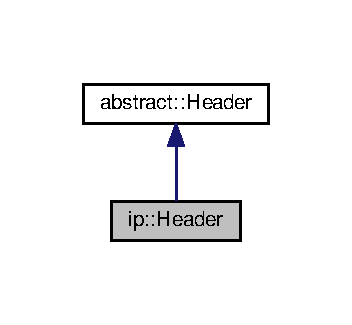
\includegraphics[width=169pt]{structip_1_1Header__inherit__graph}
\end{center}
\end{figure}


Collaboration diagram for ip\+:\+:Header\+:
\nopagebreak
\begin{figure}[H]
\begin{center}
\leavevmode
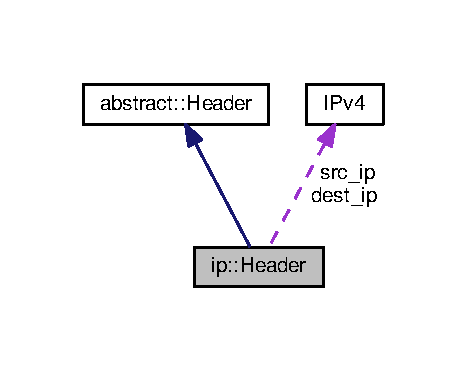
\includegraphics[width=224pt]{structip_1_1Header__coll__graph}
\end{center}
\end{figure}
\subsection*{Public Member Functions}
\begin{DoxyCompactItemize}
\item 
{\bfseries Header} (const \hyperlink{structip_1_1Header}{Header} \&other)\hypertarget{structip_1_1Header_a5e6285562e806c49a9c2f015e7400460}{}\label{structip_1_1Header_a5e6285562e806c49a9c2f015e7400460}

\item 
int {\bfseries size} () const \hypertarget{structip_1_1Header_ae426f14cf9842f7392c853463cf396da}{}\label{structip_1_1Header_ae426f14cf9842f7392c853463cf396da}

\item 
const char $\ast$ {\bfseries c\+\_\+str} () const \hypertarget{structip_1_1Header_aedc814b0cc79df651dc869d721f32b83}{}\label{structip_1_1Header_aedc814b0cc79df651dc869d721f32b83}

\item 
int {\bfseries checksum\+\_\+size} () const \hypertarget{structip_1_1Header_ae9467c8f725af565e43fb9210ad9a943}{}\label{structip_1_1Header_ae9467c8f725af565e43fb9210ad9a943}

\item 
const char $\ast$ {\bfseries checksum\+\_\+c\+\_\+str} () const \hypertarget{structip_1_1Header_a32100da1e12b3a6a8aca71d665c7a2e9}{}\label{structip_1_1Header_a32100da1e12b3a6a8aca71d665c7a2e9}

\end{DoxyCompactItemize}
\subsection*{Public Attributes}
\begin{DoxyCompactItemize}
\item 
ushort {\bfseries vide}\hypertarget{structip_1_1Header_a105b752c949ecc83a6c64dec53b51e96}{}\label{structip_1_1Header_a105b752c949ecc83a6c64dec53b51e96}

\item 
ushort {\bfseries total\+\_\+length}\hypertarget{structip_1_1Header_ae3ae0942baa2544afa8b86b9677ce464}{}\label{structip_1_1Header_ae3ae0942baa2544afa8b86b9677ce464}

\item 
ushort {\bfseries identification}\hypertarget{structip_1_1Header_a6a1db0df8e25a4bcc0f2df9549bc30b1}{}\label{structip_1_1Header_a6a1db0df8e25a4bcc0f2df9549bc30b1}

\item 
ushort {\bfseries ff}\hypertarget{structip_1_1Header_a9c79b047f8384c0e78055dda3271598f}{}\label{structip_1_1Header_a9c79b047f8384c0e78055dda3271598f}

\item 
ushort {\bfseries ttlp}\hypertarget{structip_1_1Header_ad747dde10ed8db84dd6eec3e5e6e4619}{}\label{structip_1_1Header_ad747dde10ed8db84dd6eec3e5e6e4619}

\item 
ushort {\bfseries header\+\_\+checksum}\hypertarget{structip_1_1Header_a9c970e995fa43b87ed6be2a7e3b7e179}{}\label{structip_1_1Header_a9c970e995fa43b87ed6be2a7e3b7e179}

\item 
\hyperlink{structIPv4}{I\+Pv4} {\bfseries src\+\_\+ip}\hypertarget{structip_1_1Header_a0da2fcac6244ddb22e31efb81e3571a9}{}\label{structip_1_1Header_a0da2fcac6244ddb22e31efb81e3571a9}

\item 
\hyperlink{structIPv4}{I\+Pv4} {\bfseries dest\+\_\+ip}\hypertarget{structip_1_1Header_a3609ecc70b34815e28ef2f46708fe7ee}{}\label{structip_1_1Header_a3609ecc70b34815e28ef2f46708fe7ee}

\end{DoxyCompactItemize}


The documentation for this struct was generated from the following file\+:\begin{DoxyCompactItemize}
\item 
/home/lao/powerdevs/atomics/\+Network\+D\+E\+V\+S/structures/ip.\+h\end{DoxyCompactItemize}

\hypertarget{structudp_1_1Header}{}\section{udp\+:\+:Header Struct Reference}
\label{structudp_1_1Header}\index{udp\+::\+Header@{udp\+::\+Header}}


This struct declares an \hyperlink{structudp_1_1Segment}{udp\+::\+Segment} header.  




{\ttfamily \#include $<$udp.\+h$>$}



Inheritance diagram for udp\+:\+:Header\+:\nopagebreak
\begin{figure}[H]
\begin{center}
\leavevmode
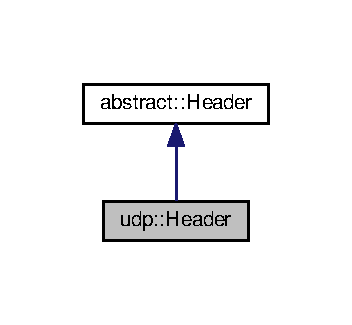
\includegraphics[width=169pt]{structudp_1_1Header__inherit__graph}
\end{center}
\end{figure}


Collaboration diagram for udp\+:\+:Header\+:\nopagebreak
\begin{figure}[H]
\begin{center}
\leavevmode
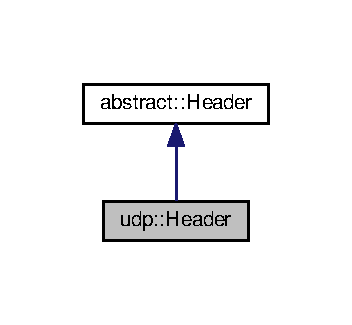
\includegraphics[width=169pt]{structudp_1_1Header__coll__graph}
\end{center}
\end{figure}
\subsection*{Public Member Functions}
\begin{DoxyCompactItemize}
\item 
\hyperlink{structudp_1_1Header_a47e86aabf149c64ede0cc55ed8888bff}{Header} ()
\begin{DoxyCompactList}\small\item\em Default constructor. \end{DoxyCompactList}\item 
\hyperlink{structudp_1_1Header_a4834b505432f80ca2eb9db6d51ab2c00}{Header} (const \hyperlink{structudp_1_1Header}{Header} \&o)
\begin{DoxyCompactList}\small\item\em Copy constructor. \end{DoxyCompactList}\item 
ushort \hyperlink{structudp_1_1Header_aeb0e9c82b2e6471758d8731ed590a502}{size} ()
\item 
const char $\ast$ \hyperlink{structudp_1_1Header_a9e39bb61a6c644edb6861f8fcb7b927d}{c\+\_\+str} ()
\begin{DoxyCompactList}\small\item\em Copy all the bytes of the instance in a memory block and return a pointer to that memory block. \end{DoxyCompactList}\end{DoxyCompactItemize}
\subsection*{Public Attributes}
\begin{DoxyCompactItemize}
\item 
ushort {\bfseries src\+\_\+port} = 0\hypertarget{structudp_1_1Header_ae751d4065b7ffd06ca2aee668efaea93}{}\label{structudp_1_1Header_ae751d4065b7ffd06ca2aee668efaea93}

\item 
ushort {\bfseries dest\+\_\+port} = 0\hypertarget{structudp_1_1Header_ac27f21b3a306cd9fbb82aa59183da569}{}\label{structudp_1_1Header_ac27f21b3a306cd9fbb82aa59183da569}

\item 
ushort {\bfseries length} = 0\hypertarget{structudp_1_1Header_abb666da1f6ca9da00addcf288b79dabe}{}\label{structudp_1_1Header_abb666da1f6ca9da00addcf288b79dabe}

\item 
ushort {\bfseries checksum} = 0\hypertarget{structudp_1_1Header_aeb4dde21af1f921c94c8fb1106dfbf05}{}\label{structudp_1_1Header_aeb4dde21af1f921c94c8fb1106dfbf05}

\end{DoxyCompactItemize}


\subsection{Detailed Description}
This struct declares an \hyperlink{structudp_1_1Segment}{udp\+::\+Segment} header. 

\begin{DoxyAuthor}{Author}
Laouen Louan Mayal Belloli 
\end{DoxyAuthor}
\begin{DoxyDate}{Date}
14 May 2017
\end{DoxyDate}
An \hyperlink{structudp_1_1Header}{udp\+::\+Header} has the next fields\+:
\begin{DoxyEnumerate}
\item src\+\_\+port\+: The local host socket port of the \hyperlink{structudp_1_1Segment}{udp\+::\+Segment}.
\item dest\+\_\+port\+: The local host socket ip of the \hyperlink{structudp_1_1Segment}{udp\+::\+Segment}.
\item length\+: The total length of the \hyperlink{structudp_1_1Segment}{udp\+::\+Segment}.
\item checksum\+: The checksum used to verify the \hyperlink{structudp_1_1Segment}{udp\+::\+Segment} has correctly arrived. 
\end{DoxyEnumerate}

\subsection{Constructor \& Destructor Documentation}
\index{udp\+::\+Header@{udp\+::\+Header}!Header@{Header}}
\index{Header@{Header}!udp\+::\+Header@{udp\+::\+Header}}
\subsubsection[{\texorpdfstring{Header()}{Header()}}]{\setlength{\rightskip}{0pt plus 5cm}udp\+::\+Header\+::\+Header (
\begin{DoxyParamCaption}
{}
\end{DoxyParamCaption}
)\hspace{0.3cm}{\ttfamily [inline]}}\hypertarget{structudp_1_1Header_a47e86aabf149c64ede0cc55ed8888bff}{}\label{structudp_1_1Header_a47e86aabf149c64ede0cc55ed8888bff}


Default constructor. 

Construct an empty new instance. \index{udp\+::\+Header@{udp\+::\+Header}!Header@{Header}}
\index{Header@{Header}!udp\+::\+Header@{udp\+::\+Header}}
\subsubsection[{\texorpdfstring{Header(const Header \&o)}{Header(const Header &o)}}]{\setlength{\rightskip}{0pt plus 5cm}udp\+::\+Header\+::\+Header (
\begin{DoxyParamCaption}
\item[{const {\bf Header} \&}]{o}
\end{DoxyParamCaption}
)\hspace{0.3cm}{\ttfamily [inline]}}\hypertarget{structudp_1_1Header_a4834b505432f80ca2eb9db6d51ab2c00}{}\label{structudp_1_1Header_a4834b505432f80ca2eb9db6d51ab2c00}


Copy constructor. 

Construct a new instance with a copy of the instance passed as parameter.


\begin{DoxyParams}{Parameters}
{\em o} & An \hyperlink{structudp_1_1Header}{udp\+::\+Header} to copy in the new instance. \\
\hline
\end{DoxyParams}


\subsection{Member Function Documentation}
\index{udp\+::\+Header@{udp\+::\+Header}!c\+\_\+str@{c\+\_\+str}}
\index{c\+\_\+str@{c\+\_\+str}!udp\+::\+Header@{udp\+::\+Header}}
\subsubsection[{\texorpdfstring{c\+\_\+str()}{c_str()}}]{\setlength{\rightskip}{0pt plus 5cm}const char$\ast$ udp\+::\+Header\+::c\+\_\+str (
\begin{DoxyParamCaption}
{}
\end{DoxyParamCaption}
)\hspace{0.3cm}{\ttfamily [inline]}}\hypertarget{structudp_1_1Header_a9e39bb61a6c644edb6861f8fcb7b927d}{}\label{structudp_1_1Header_a9e39bb61a6c644edb6861f8fcb7b927d}


Copy all the bytes of the instance in a memory block and return a pointer to that memory block. 

\begin{DoxyReturn}{Returns}
A const char $\ast$ that point to the memory block where the instance was capied. 
\end{DoxyReturn}
\index{udp\+::\+Header@{udp\+::\+Header}!size@{size}}
\index{size@{size}!udp\+::\+Header@{udp\+::\+Header}}
\subsubsection[{\texorpdfstring{size()}{size()}}]{\setlength{\rightskip}{0pt plus 5cm}ushort udp\+::\+Header\+::size (
\begin{DoxyParamCaption}
{}
\end{DoxyParamCaption}
)\hspace{0.3cm}{\ttfamily [inline]}}\hypertarget{structudp_1_1Header_aeb0e9c82b2e6471758d8731ed590a502}{}\label{structudp_1_1Header_aeb0e9c82b2e6471758d8731ed590a502}
\begin{DoxyReturn}{Returns}
Returns the instance size in bytes 
\end{DoxyReturn}


The documentation for this struct was generated from the following file\+:\begin{DoxyCompactItemize}
\item 
/home/lao/powerdevs/atomics/\+Network\+D\+E\+V\+S/structures/udp.\+h\end{DoxyCompactItemize}

\hypertarget{classinput__stream}{}\section{input\+\_\+stream$<$ I\+N\+P\+UT $>$ Class Template Reference}
\label{classinput__stream}\index{input\+\_\+stream$<$ I\+N\+P\+U\+T $>$@{input\+\_\+stream$<$ I\+N\+P\+U\+T $>$}}


Template meta model of an \hyperlink{classinput__stream}{input\+\_\+stream} model. Once instanciated, this model is initialized with a file\+\_\+path pointing to the file where is the input to generate and insert to the model. This model parses the file lines using the \hyperlink{classParser}{parser} class and generates a timed input that will be send through the output port number zero. The input stream uses the next\+\_\+timed\+\_\+input method from the \hyperlink{classParser}{parser} class in order to read the input with it asociated time as the first value of each line (see the \hyperlink{classParser}{parser} documentation).  




{\ttfamily \#include $<$input\+\_\+stream.\+h$>$}



Inheritance diagram for input\+\_\+stream$<$ I\+N\+P\+UT $>$\+:\nopagebreak
\begin{figure}[H]
\begin{center}
\leavevmode
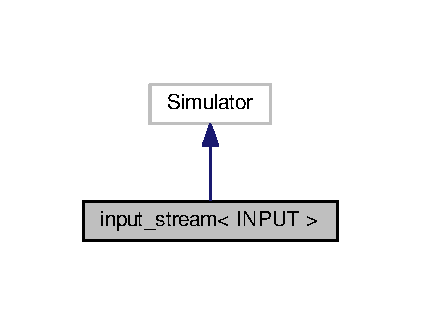
\includegraphics[width=202pt]{classinput__stream__inherit__graph}
\end{center}
\end{figure}


Collaboration diagram for input\+\_\+stream$<$ I\+N\+P\+UT $>$\+:\nopagebreak
\begin{figure}[H]
\begin{center}
\leavevmode
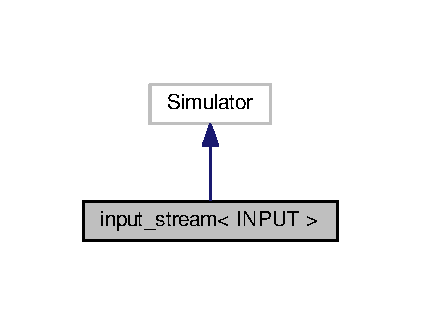
\includegraphics[width=202pt]{classinput__stream__coll__graph}
\end{center}
\end{figure}
\subsection*{Public Member Functions}
\begin{DoxyCompactItemize}
\item 
{\bfseries input\+\_\+stream} (const char $\ast$n)\hypertarget{classinput__stream_ac5075c6ed0a87da7a096fd44cbc4d113}{}\label{classinput__stream_ac5075c6ed0a87da7a096fd44cbc4d113}

\item 
void {\bfseries init} (double t,...)\hypertarget{classinput__stream_a7080ba1b96056747cbd0f836b692e319}{}\label{classinput__stream_a7080ba1b96056747cbd0f836b692e319}

\item 
double {\bfseries ta} (double t)\hypertarget{classinput__stream_a2646cf888bb02ff289b99c473420c474}{}\label{classinput__stream_a2646cf888bb02ff289b99c473420c474}

\item 
void {\bfseries dint} (double t)\hypertarget{classinput__stream_a6587dc4c03edab458b160fa9e0fc26a9}{}\label{classinput__stream_a6587dc4c03edab458b160fa9e0fc26a9}

\item 
void {\bfseries dext} (Event x, double t)\hypertarget{classinput__stream_add1e66ac8a04594931a57387681e6131}{}\label{classinput__stream_add1e66ac8a04594931a57387681e6131}

\item 
Event {\bfseries lambda} (double t)\hypertarget{classinput__stream_ac4ba4f32f1d91c8790b087c3020a4ccf}{}\label{classinput__stream_ac4ba4f32f1d91c8790b087c3020a4ccf}

\item 
void {\bfseries exit} ()\hypertarget{classinput__stream_a74fc7095691b7da697d8008ea783ae23}{}\label{classinput__stream_a74fc7095691b7da697d8008ea783ae23}

\end{DoxyCompactItemize}


\subsection{Detailed Description}
\subsubsection*{template$<$typename I\+N\+P\+UT$>$\\*
class input\+\_\+stream$<$ I\+N\+P\+U\+T $>$}

Template meta model of an \hyperlink{classinput__stream}{input\+\_\+stream} model. Once instanciated, this model is initialized with a file\+\_\+path pointing to the file where is the input to generate and insert to the model. This model parses the file lines using the \hyperlink{classParser}{parser} class and generates a timed input that will be send through the output port number zero. The input stream uses the next\+\_\+timed\+\_\+input method from the \hyperlink{classParser}{parser} class in order to read the input with it asociated time as the first value of each line (see the \hyperlink{classParser}{parser} documentation). 

\begin{DoxyAuthor}{Author}
Laouen Louan Mayal Belloli 
\end{DoxyAuthor}
\begin{DoxyDate}{Date}
14 May 2017
\end{DoxyDate}
This model must be inherited by a new class with the template D\+A\+TA parameter specified with the input type to generate.

The new class must follow the Power\+D\+E\+VS specifications and a .cpp file must exist even if it is an empty file in order to correctly compile the model from the Power\+D\+E\+VS I\+DE.

The next rules must be followed\+:
\begin{DoxyEnumerate}
\item This file must be included in the file where the new class is declared.
\item The new class name must be all lower case.
\item The new class must have in the first line the next comment\+: //\+C\+PP\+:network\+D\+E\+V\+S/new\+\_\+class\+\_\+name.\+cpp.
\item The file network\+D\+E\+V\+S/new\+\_\+class\+\_\+name.\+cpp must exist as an empty file.
\item The constructor of the new class must be specified in the public section as shown here\+: new\+\_\+class\+\_\+name(const char $\ast$n)\+: \hyperlink{classinput__stream}{input\+\_\+stream(n)} \{\};
\end{DoxyEnumerate}

The parameters to specifie in the Power\+D\+E\+VS I\+DE (right click in the atomic model -\/$>$ edit -\/$>$ parameters) are the nexts\+:

\tabulinesep=1mm
\begin{longtabu} spread 0pt [c]{*3{|X[-1]}|}
\hline
\rowcolor{\tableheadbgcolor}\PBS\centering {\bf name }&\PBS\centering {\bf type }&\PBS\centering {\bf description  }\\\cline{1-3}
\endfirsthead
\hline
\endfoot
\hline
\rowcolor{\tableheadbgcolor}\PBS\centering {\bf name }&\PBS\centering {\bf type }&\PBS\centering {\bf description  }\\\cline{1-3}
\endhead
\PBS\centering module name &\PBS\centering String &\PBS\centering a name used to tag the logs generated by this model \\\cline{1-3}
\PBS\centering file path &\PBS\centering String &\PBS\centering the file path from where to read the input \\\cline{1-3}
\end{longtabu}

\begin{DoxyTemplParams}{Template Parameters}
{\em D\+A\+TA} & The data type of the input to generate. Must implement the $>$$>$ operator. \\
\hline
\end{DoxyTemplParams}


The documentation for this class was generated from the following file\+:\begin{DoxyCompactItemize}
\item 
/home/lao/\+Documents/git/\+Network\+D\+E\+V\+S/template/input\+\_\+stream.\+h\end{DoxyCompactItemize}

\hypertarget{classip__control__src}{}\section{ip\+\_\+control\+\_\+src Class Reference}
\label{classip__control__src}\index{ip\+\_\+control\+\_\+src@{ip\+\_\+control\+\_\+src}}


A specialization of \hyperlink{classinput__stream}{input\+\_\+stream} template model to generate input of type \hyperlink{structip_1_1Control}{ip\+::\+Control} from a file.  




{\ttfamily \#include $<$ip\+\_\+control\+\_\+src.\+h$>$}



Inheritance diagram for ip\+\_\+control\+\_\+src\+:\nopagebreak
\begin{figure}[H]
\begin{center}
\leavevmode
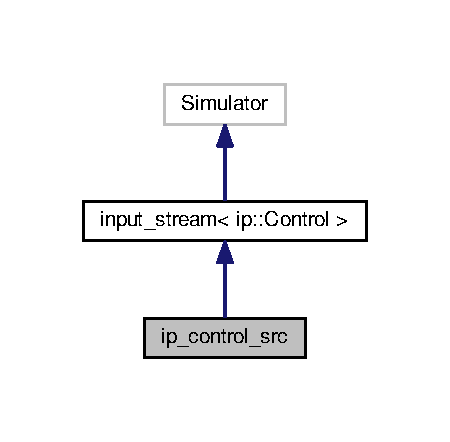
\includegraphics[width=216pt]{classip__control__src__inherit__graph}
\end{center}
\end{figure}


Collaboration diagram for ip\+\_\+control\+\_\+src\+:\nopagebreak
\begin{figure}[H]
\begin{center}
\leavevmode
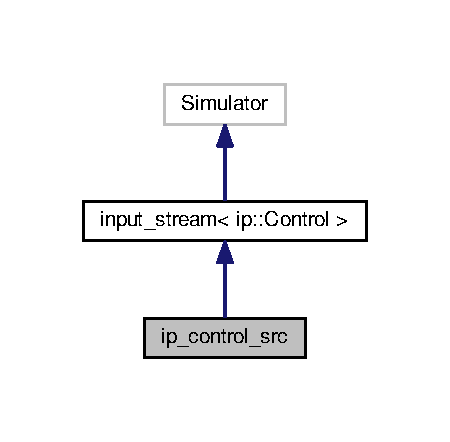
\includegraphics[width=216pt]{classip__control__src__coll__graph}
\end{center}
\end{figure}
\subsection*{Public Member Functions}
\begin{DoxyCompactItemize}
\item 
{\bfseries ip\+\_\+control\+\_\+src} (const char $\ast$n)\hypertarget{classip__control__src_a6046f82b5fd050f6ae6f24910f4a2a3c}{}\label{classip__control__src_a6046f82b5fd050f6ae6f24910f4a2a3c}

\end{DoxyCompactItemize}


\subsection{Detailed Description}
A specialization of \hyperlink{classinput__stream}{input\+\_\+stream} template model to generate input of type \hyperlink{structip_1_1Control}{ip\+::\+Control} from a file. 

\begin{DoxyAuthor}{Author}
Lauen Louan Mayal Belloli 
\end{DoxyAuthor}
\begin{DoxyDate}{Date}
14 May 2017 
\end{DoxyDate}


The documentation for this class was generated from the following file\+:\begin{DoxyCompactItemize}
\item 
/home/lao/\+Documents/git/\+Network\+D\+E\+V\+S/ip\+\_\+control\+\_\+src.\+h\end{DoxyCompactItemize}

\hypertarget{classip__datagram__sink}{}\section{ip\+\_\+datagram\+\_\+sink Class Reference}
\label{classip__datagram__sink}\index{ip\+\_\+datagram\+\_\+sink@{ip\+\_\+datagram\+\_\+sink}}


A specialization of \hyperlink{classoutput__stream}{output\+\_\+stream} template model to write in a file output messages of type \hyperlink{structip_1_1Datagram}{ip\+::\+Datagram}.  




{\ttfamily \#include $<$ip\+\_\+datagram\+\_\+sink.\+h$>$}



Inheritance diagram for ip\+\_\+datagram\+\_\+sink\+:\nopagebreak
\begin{figure}[H]
\begin{center}
\leavevmode
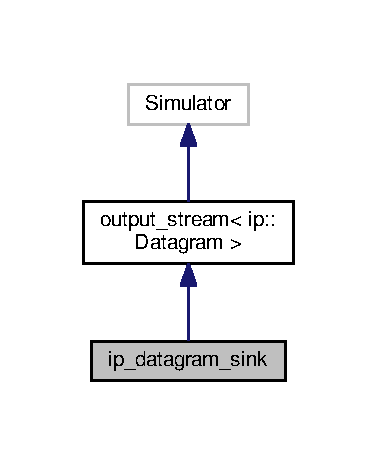
\includegraphics[width=181pt]{classip__datagram__sink__inherit__graph}
\end{center}
\end{figure}


Collaboration diagram for ip\+\_\+datagram\+\_\+sink\+:\nopagebreak
\begin{figure}[H]
\begin{center}
\leavevmode
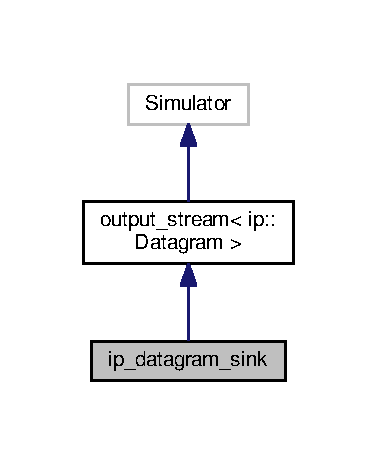
\includegraphics[width=181pt]{classip__datagram__sink__coll__graph}
\end{center}
\end{figure}
\subsection*{Public Member Functions}
\begin{DoxyCompactItemize}
\item 
{\bfseries ip\+\_\+datagram\+\_\+sink} (const char $\ast$n)\hypertarget{classip__datagram__sink_a660e2f26390312a94d8e4a2fbc0e4614}{}\label{classip__datagram__sink_a660e2f26390312a94d8e4a2fbc0e4614}

\end{DoxyCompactItemize}


\subsection{Detailed Description}
A specialization of \hyperlink{classoutput__stream}{output\+\_\+stream} template model to write in a file output messages of type \hyperlink{structip_1_1Datagram}{ip\+::\+Datagram}. 

\begin{DoxyAuthor}{Author}
Lauen Louan Mayal Belloli 
\end{DoxyAuthor}
\begin{DoxyDate}{Date}
14 May 2017 
\end{DoxyDate}


The documentation for this class was generated from the following file\+:\begin{DoxyCompactItemize}
\item 
/home/lao/powerdevs/atomics/\+Network\+D\+E\+V\+S/ip\+\_\+datagram\+\_\+sink.\+h\end{DoxyCompactItemize}

\hypertarget{classip__datagram__src}{}\section{ip\+\_\+datagram\+\_\+src Class Reference}
\label{classip__datagram__src}\index{ip\+\_\+datagram\+\_\+src@{ip\+\_\+datagram\+\_\+src}}


Inheritance diagram for ip\+\_\+datagram\+\_\+src\+:\nopagebreak
\begin{figure}[H]
\begin{center}
\leavevmode
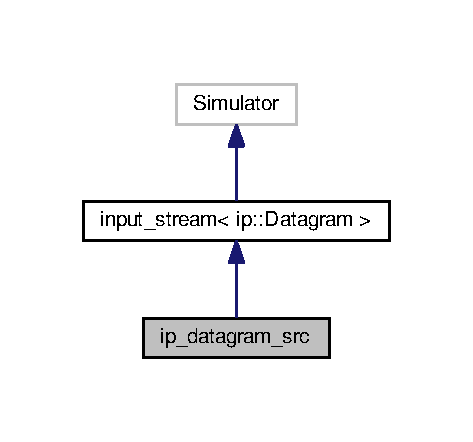
\includegraphics[width=227pt]{classip__datagram__src__inherit__graph}
\end{center}
\end{figure}


Collaboration diagram for ip\+\_\+datagram\+\_\+src\+:\nopagebreak
\begin{figure}[H]
\begin{center}
\leavevmode
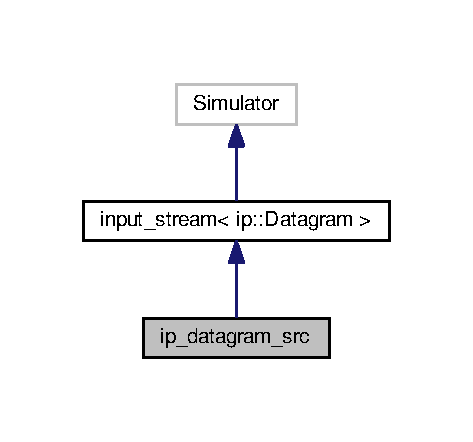
\includegraphics[width=227pt]{classip__datagram__src__coll__graph}
\end{center}
\end{figure}
\subsection*{Public Member Functions}
\begin{DoxyCompactItemize}
\item 
{\bfseries ip\+\_\+datagram\+\_\+src} (const char $\ast$n)\hypertarget{classip__datagram__src_a06b73f2700abc04cf41be7e0872e134e}{}\label{classip__datagram__src_a06b73f2700abc04cf41be7e0872e134e}

\end{DoxyCompactItemize}


The documentation for this class was generated from the following file\+:\begin{DoxyCompactItemize}
\item 
/home/lao/powerdevs/atomics/\+Network\+D\+E\+V\+S/ip\+\_\+datagram\+\_\+src.\+h\end{DoxyCompactItemize}

\hypertarget{classip__host__protocol}{}\section{ip\+\_\+host\+\_\+protocol Class Reference}
\label{classip__host__protocol}\index{ip\+\_\+host\+\_\+protocol@{ip\+\_\+host\+\_\+protocol}}


Inheritance diagram for ip\+\_\+host\+\_\+protocol\+:\nopagebreak
\begin{figure}[H]
\begin{center}
\leavevmode
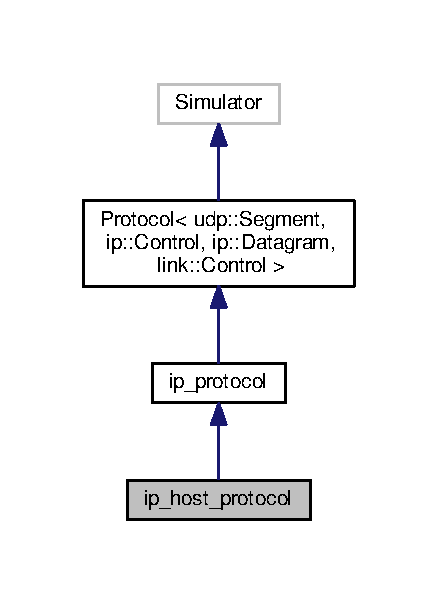
\includegraphics[width=350pt]{classip__host__protocol__inherit__graph}
\end{center}
\end{figure}


Collaboration diagram for ip\+\_\+host\+\_\+protocol\+:\nopagebreak
\begin{figure}[H]
\begin{center}
\leavevmode
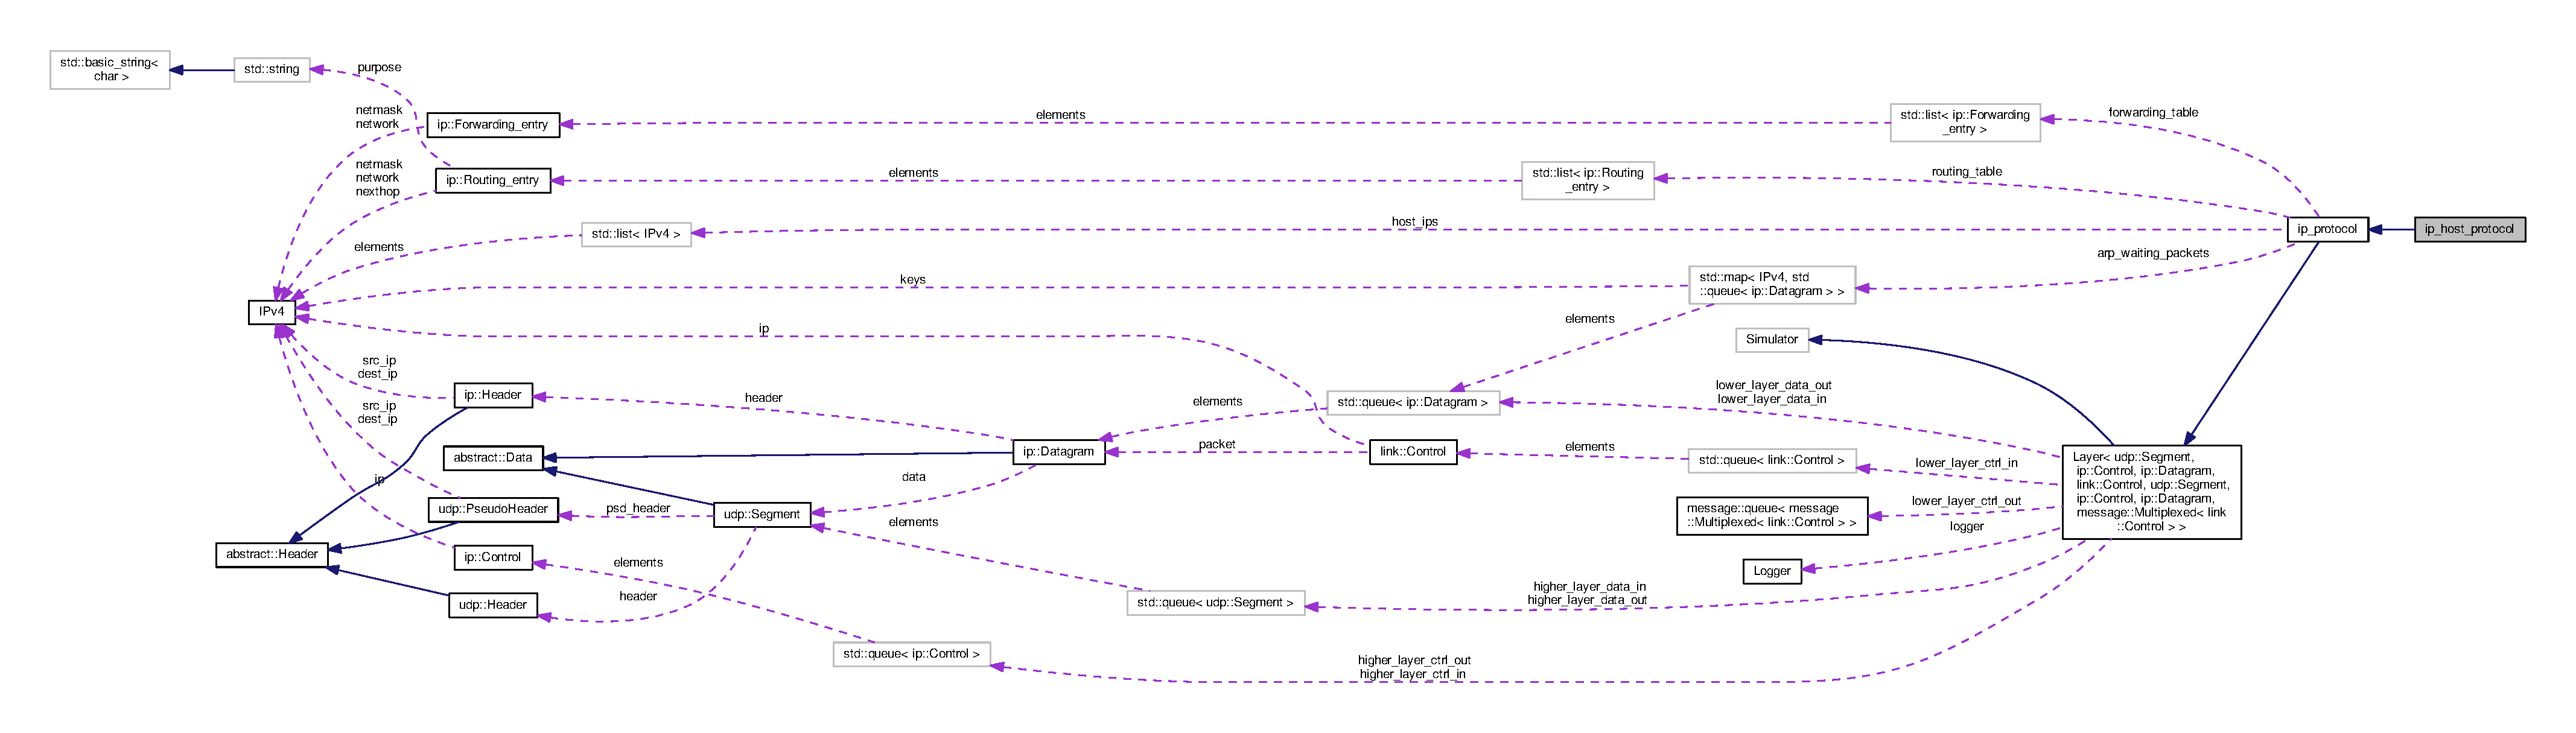
\includegraphics[width=350pt]{classip__host__protocol__coll__graph}
\end{center}
\end{figure}
\subsection*{Public Member Functions}
\begin{DoxyCompactItemize}
\item 
{\bfseries ip\+\_\+host\+\_\+protocol} (const char $\ast$n)\hypertarget{classip__host__protocol_a29412893a5845c69af6031eb6734e8c0}{}\label{classip__host__protocol_a29412893a5845c69af6031eb6734e8c0}

\item 
virtual void {\bfseries dinternal} (double)\hypertarget{classip__host__protocol_a2e2c43aeb81ae38702b7dec6f7df9227}{}\label{classip__host__protocol_a2e2c43aeb81ae38702b7dec6f7df9227}

\end{DoxyCompactItemize}
\subsection*{Additional Inherited Members}


The documentation for this class was generated from the following files\+:\begin{DoxyCompactItemize}
\item 
/home/lao/powerdevs/atomics/\+Network\+D\+E\+V\+S/ip\+\_\+host\+\_\+protocol.\+h\item 
/home/lao/powerdevs/atomics/\+Network\+D\+E\+V\+S/ip\+\_\+host\+\_\+protocol.\+cpp\end{DoxyCompactItemize}

\hypertarget{classip__protocol}{}\section{ip\+\_\+protocol Class Reference}
\label{classip__protocol}\index{ip\+\_\+protocol@{ip\+\_\+protocol}}


Inheritance diagram for ip\+\_\+protocol\+:\nopagebreak
\begin{figure}[H]
\begin{center}
\leavevmode
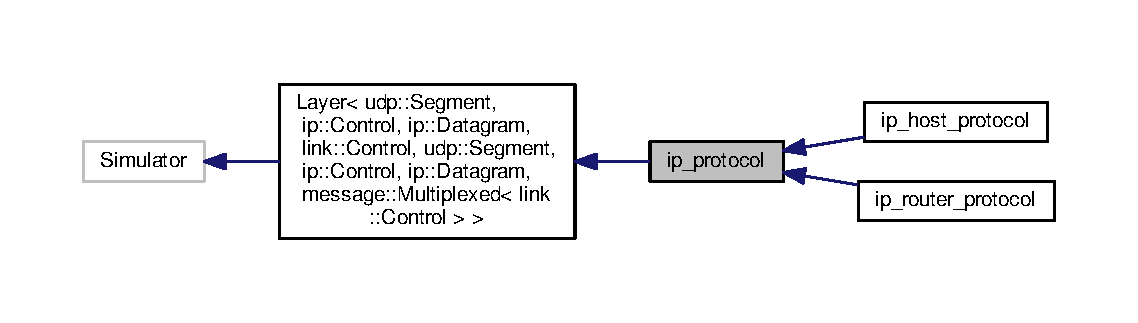
\includegraphics[width=280pt]{classip__protocol__inherit__graph}
\end{center}
\end{figure}


Collaboration diagram for ip\+\_\+protocol\+:\nopagebreak
\begin{figure}[H]
\begin{center}
\leavevmode
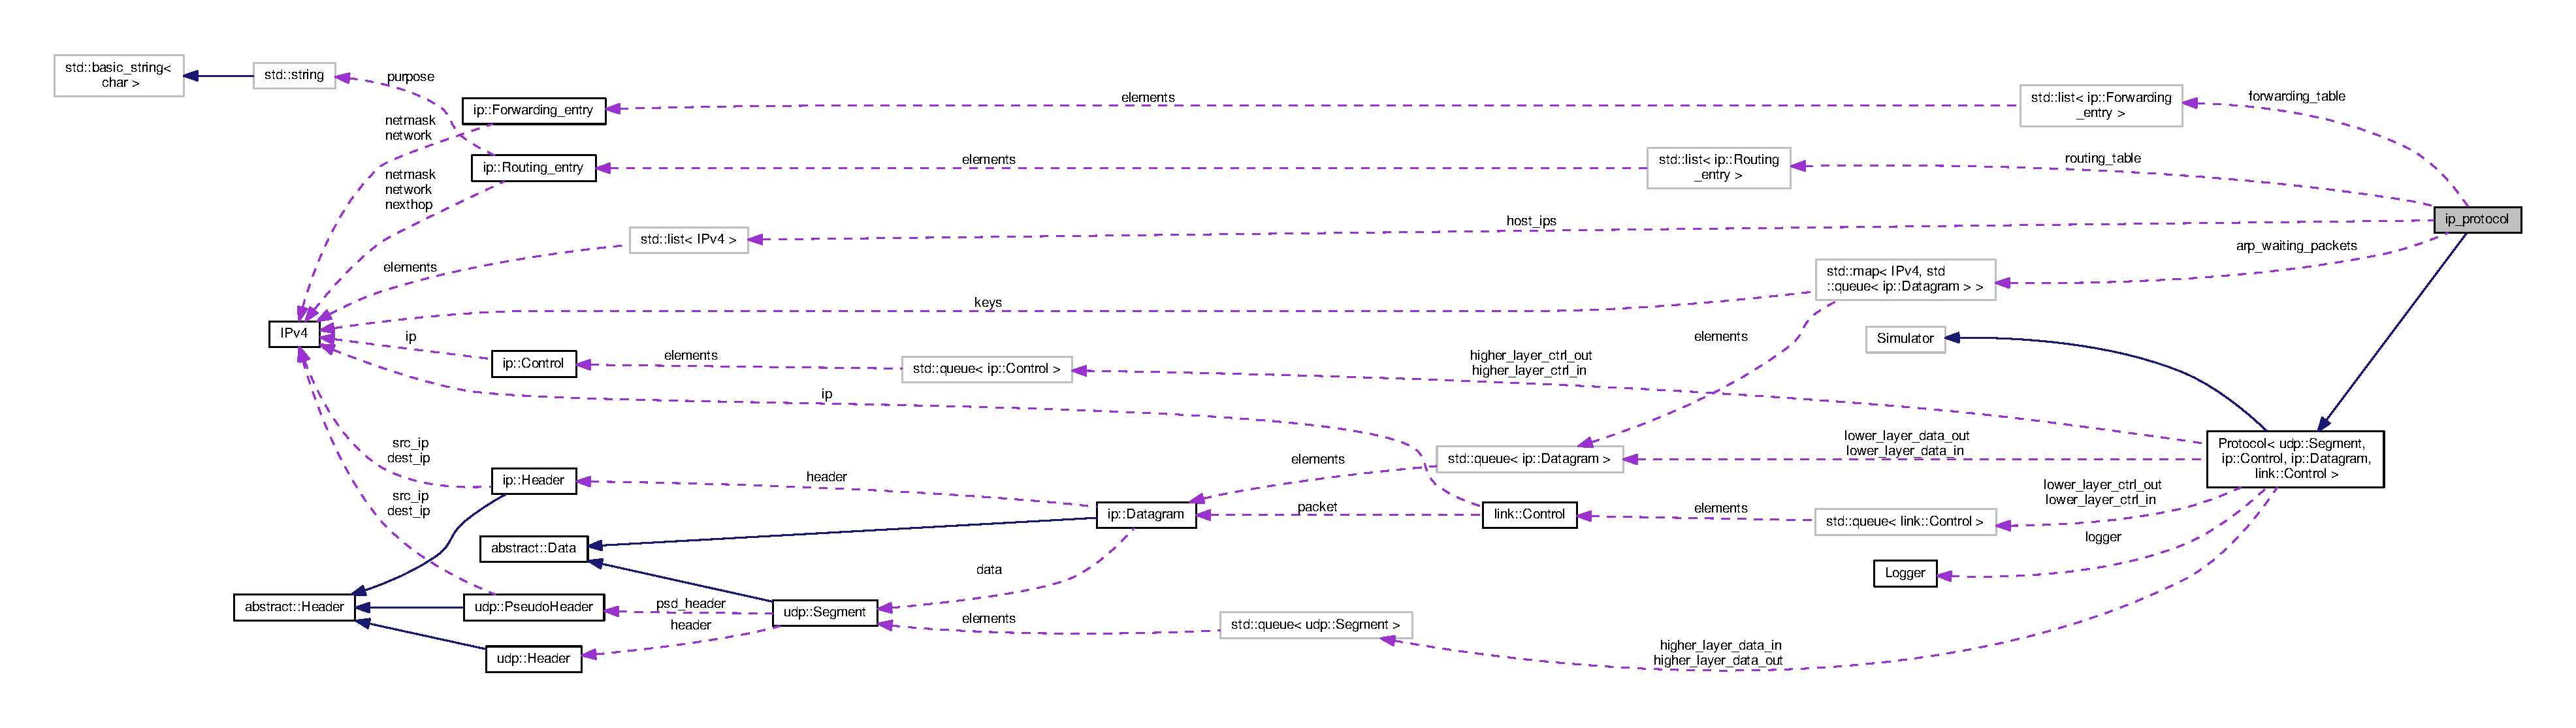
\includegraphics[width=350pt]{classip__protocol__coll__graph}
\end{center}
\end{figure}
\subsection*{Public Member Functions}
\begin{DoxyCompactItemize}
\item 
{\bfseries ip\+\_\+protocol} (const char $\ast$n)\hypertarget{classip__protocol_af3d5fa13a4175ab93d431ad38e7c3712}{}\label{classip__protocol_af3d5fa13a4175ab93d431ad38e7c3712}

\item 
void {\bfseries init} (double,...)\hypertarget{classip__protocol_a41b4678b7d525775ca4ed84dd4f8daac}{}\label{classip__protocol_a41b4678b7d525775ca4ed84dd4f8daac}

\item 
double {\bfseries ta} (double t)\hypertarget{classip__protocol_a799af7a028afc688255e9efe732e00f4}{}\label{classip__protocol_a799af7a028afc688255e9efe732e00f4}

\item 
Event {\bfseries lambda} (double)\hypertarget{classip__protocol_ae92e4088780f38a62419a202d53e2511}{}\label{classip__protocol_ae92e4088780f38a62419a202d53e2511}

\item 
void {\bfseries exit} ()\hypertarget{classip__protocol_aed94f19da59b71685e9d17de4febcd75}{}\label{classip__protocol_aed94f19da59b71685e9d17de4febcd75}

\item 
virtual void \hyperlink{classip__protocol_a5c4dd62ee8cffa83a592f29306686be9}{dinternal} (double)
\begin{DoxyCompactList}\small\item\em This method is virtual and must be overloaded with the protocol. \end{DoxyCompactList}\item 
virtual void \hyperlink{classip__protocol_a34e2cc9e802edf0ba1fdbcbcbee92f5b}{dexternal} (double)
\begin{DoxyCompactList}\small\item\em This method is virtual and can be overloaded with the protocol. \end{DoxyCompactList}\end{DoxyCompactItemize}
\subsection*{Protected Member Functions}
\begin{DoxyCompactItemize}
\item 
void {\bfseries route\+I\+P\+Datagram} (\hyperlink{structip_1_1Datagram}{ip\+::\+Datagram})\hypertarget{classip__protocol_ae49db3617f34c1765b8b3f64996fe7eb}{}\label{classip__protocol_ae49db3617f34c1765b8b3f64996fe7eb}

\item 
void {\bfseries arp} (\hyperlink{structip_1_1Datagram}{ip\+::\+Datagram}, \hyperlink{structIPv4}{I\+Pv4})\hypertarget{classip__protocol_a32a4c86b4f32594b60a3f7170421fb7e}{}\label{classip__protocol_a32a4c86b4f32594b60a3f7170421fb7e}

\item 
void {\bfseries process\+Link\+Control} (\hyperlink{structlink_1_1Control}{link\+::\+Control})\hypertarget{classip__protocol_a6c03ee07d8fa8c2b4a5f43732fb95c05}{}\label{classip__protocol_a6c03ee07d8fa8c2b4a5f43732fb95c05}

\item 
ushort {\bfseries calculate\+Checksum} (\hyperlink{structip_1_1Header}{ip\+::\+Header}) const \hypertarget{classip__protocol_a14d8f57ecf3e4e7b8c2fc5b98a782939}{}\label{classip__protocol_a14d8f57ecf3e4e7b8c2fc5b98a782939}

\item 
bool {\bfseries verifychecksum} (\hyperlink{structip_1_1Header}{ip\+::\+Header}) const \hypertarget{classip__protocol_aa730a2a5c453742c1a3bcc105bc839c0}{}\label{classip__protocol_aa730a2a5c453742c1a3bcc105bc839c0}

\item 
bool {\bfseries matches\+Host\+Ips} (\hyperlink{structIPv4}{I\+Pv4}) const \hypertarget{classip__protocol_ac83406e9e5d5e54b1a3afd4d5a4f53c9}{}\label{classip__protocol_ac83406e9e5d5e54b1a3afd4d5a4f53c9}

\item 
bool {\bfseries get\+Best\+Route} (\hyperlink{structIPv4}{I\+Pv4}, \hyperlink{structip_1_1Routing__entry}{ip\+::\+Routing\+\_\+entry} \&) const \hypertarget{classip__protocol_a391caec68e7eaf86659f0479763500ec}{}\label{classip__protocol_a391caec68e7eaf86659f0479763500ec}

\item 
bool {\bfseries is\+Best\+Route} (\hyperlink{structip_1_1Routing__entry}{ip\+::\+Routing\+\_\+entry}, \hyperlink{structip_1_1Routing__entry}{ip\+::\+Routing\+\_\+entry}) const \hypertarget{classip__protocol_a49ccaaab6a679045ddbff00f44ca49cc}{}\label{classip__protocol_a49ccaaab6a679045ddbff00f44ca49cc}

\item 
bool {\bfseries get\+Interface} (\hyperlink{structIPv4}{I\+Pv4}, ushort \&) const \hypertarget{classip__protocol_a15e87109b4478fe5028e3e67c11a20fb}{}\label{classip__protocol_a15e87109b4478fe5028e3e67c11a20fb}

\end{DoxyCompactItemize}
\subsection*{Protected Attributes}
\begin{DoxyCompactItemize}
\item 
std\+::list$<$ \hyperlink{structip_1_1Forwarding__entry}{ip\+::\+Forwarding\+\_\+entry} $>$ {\bfseries forwarding\+\_\+table}\hypertarget{classip__protocol_aaeb5d99cd92641500f0013e3822d56a1}{}\label{classip__protocol_aaeb5d99cd92641500f0013e3822d56a1}

\item 
std\+::map$<$ \hyperlink{structIPv4}{I\+Pv4}, std\+::queue$<$ \hyperlink{structip_1_1Datagram}{ip\+::\+Datagram} $>$ $>$ {\bfseries arp\+\_\+waiting\+\_\+packets}\hypertarget{classip__protocol_a284258e9e9050ae7e51b3864f5a953ce}{}\label{classip__protocol_a284258e9e9050ae7e51b3864f5a953ce}

\item 
std\+::list$<$ \hyperlink{structIPv4}{I\+Pv4} $>$ {\bfseries host\+\_\+ips}\hypertarget{classip__protocol_aa7d9cb9aba71a12d55cbb48ebb8023bf}{}\label{classip__protocol_aa7d9cb9aba71a12d55cbb48ebb8023bf}

\item 
std\+::list$<$ \hyperlink{structip_1_1Routing__entry}{ip\+::\+Routing\+\_\+entry} $>$ {\bfseries routing\+\_\+table}\hypertarget{classip__protocol_a10115583b02359dd2a5670d1ad15f491}{}\label{classip__protocol_a10115583b02359dd2a5670d1ad15f491}

\item 
double {\bfseries process\+\_\+udp\+\_\+segment\+\_\+time} = 70\hypertarget{classip__protocol_a70dbab92c8f81ef06fd54f3e8d7bd948}{}\label{classip__protocol_a70dbab92c8f81ef06fd54f3e8d7bd948}

\item 
double {\bfseries process\+\_\+ip\+\_\+datagram\+\_\+time} = 70\hypertarget{classip__protocol_a5a4799b4959601058134ada5e68535d9}{}\label{classip__protocol_a5a4799b4959601058134ada5e68535d9}

\item 
double {\bfseries process\+\_\+link\+\_\+control\+\_\+time} = 70\hypertarget{classip__protocol_a5d8f0b585621473601c220ad283a825f}{}\label{classip__protocol_a5d8f0b585621473601c220ad283a825f}

\item 
double {\bfseries send\+\_\+frame\+\_\+time} = 10\hypertarget{classip__protocol_a228a55f7b2c25fa8e3900893ccc87e41}{}\label{classip__protocol_a228a55f7b2c25fa8e3900893ccc87e41}

\end{DoxyCompactItemize}


\subsection{Member Function Documentation}
\index{ip\+\_\+protocol@{ip\+\_\+protocol}!dexternal@{dexternal}}
\index{dexternal@{dexternal}!ip\+\_\+protocol@{ip\+\_\+protocol}}
\subsubsection[{\texorpdfstring{dexternal(double)}{dexternal(double)}}]{\setlength{\rightskip}{0pt plus 5cm}virtual void ip\+\_\+protocol\+::dexternal (
\begin{DoxyParamCaption}
\item[{double}]{t}
\end{DoxyParamCaption}
)\hspace{0.3cm}{\ttfamily [inline]}, {\ttfamily [virtual]}}\hypertarget{classip__protocol_a34e2cc9e802edf0ba1fdbcbcbee92f5b}{}\label{classip__protocol_a34e2cc9e802edf0ba1fdbcbcbee92f5b}


This method is virtual and can be overloaded with the protocol. 

This method is called each time an external transition takes place.


\begin{DoxyParams}{Parameters}
{\em t} & The virtual global time of the simulation at which the method is triggered. \\
\hline
\end{DoxyParams}


Reimplemented from \hyperlink{classProtocol_a9995a053fa35d5cd45f609958c6529b2}{Protocol$<$ udp\+::\+Segment, ip\+::\+Control, ip\+::\+Datagram, link\+::\+Control $>$}.

\index{ip\+\_\+protocol@{ip\+\_\+protocol}!dinternal@{dinternal}}
\index{dinternal@{dinternal}!ip\+\_\+protocol@{ip\+\_\+protocol}}
\subsubsection[{\texorpdfstring{dinternal(double)}{dinternal(double)}}]{\setlength{\rightskip}{0pt plus 5cm}virtual void ip\+\_\+protocol\+::dinternal (
\begin{DoxyParamCaption}
\item[{double}]{t}
\end{DoxyParamCaption}
)\hspace{0.3cm}{\ttfamily [inline]}, {\ttfamily [virtual]}}\hypertarget{classip__protocol_a5c4dd62ee8cffa83a592f29306686be9}{}\label{classip__protocol_a5c4dd62ee8cffa83a592f29306686be9}


This method is virtual and must be overloaded with the protocol. 

This method is called while the input queues has messages to process and the procotol should be implemented here..


\begin{DoxyParams}{Parameters}
{\em t} & The virtual global time of the simulation at which the method is triggered. \\
\hline
\end{DoxyParams}


Reimplemented from \hyperlink{classProtocol_a9c6247fa4ea8524d1214fca4cacbd781}{Protocol$<$ udp\+::\+Segment, ip\+::\+Control, ip\+::\+Datagram, link\+::\+Control $>$}.



Reimplemented in \hyperlink{classip__router__protocol_a14cf3c7e1418ee8c6035b79626f99438}{ip\+\_\+router\+\_\+protocol}, and \hyperlink{classip__host__protocol_a2e2c43aeb81ae38702b7dec6f7df9227}{ip\+\_\+host\+\_\+protocol}.



The documentation for this class was generated from the following files\+:\begin{DoxyCompactItemize}
\item 
/home/lao/powerdevs/atomics/\+Network\+D\+E\+V\+S/ip\+\_\+protocol.\+h\item 
/home/lao/powerdevs/atomics/\+Network\+D\+E\+V\+S/ip\+\_\+protocol.\+cpp\end{DoxyCompactItemize}

\hypertarget{classip__router__protocol}{}\section{ip\+\_\+router\+\_\+protocol Class Reference}
\label{classip__router__protocol}\index{ip\+\_\+router\+\_\+protocol@{ip\+\_\+router\+\_\+protocol}}


Inheritance diagram for ip\+\_\+router\+\_\+protocol\+:\nopagebreak
\begin{figure}[H]
\begin{center}
\leavevmode
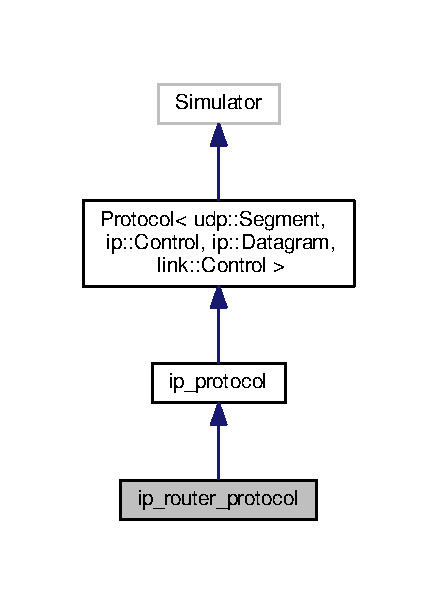
\includegraphics[width=350pt]{classip__router__protocol__inherit__graph}
\end{center}
\end{figure}


Collaboration diagram for ip\+\_\+router\+\_\+protocol\+:\nopagebreak
\begin{figure}[H]
\begin{center}
\leavevmode
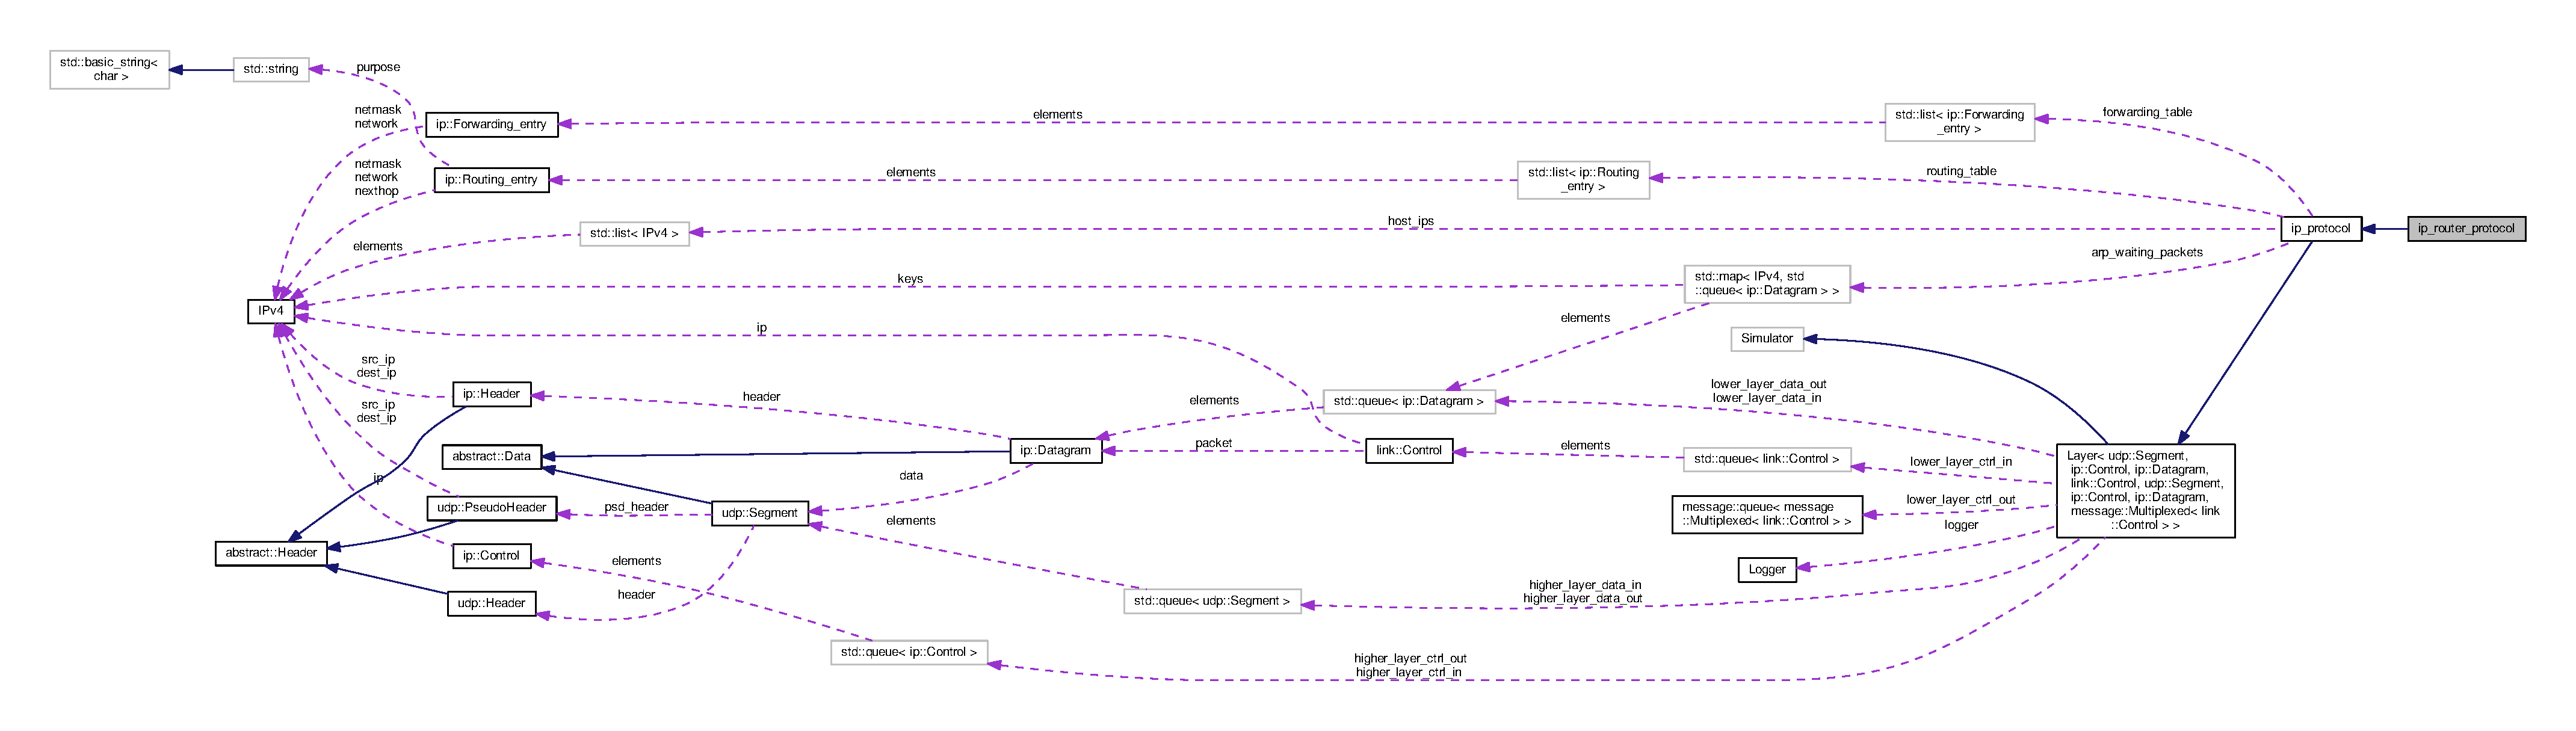
\includegraphics[width=350pt]{classip__router__protocol__coll__graph}
\end{center}
\end{figure}
\subsection*{Public Member Functions}
\begin{DoxyCompactItemize}
\item 
{\bfseries ip\+\_\+router\+\_\+protocol} (const char $\ast$n)\hypertarget{classip__router__protocol_ada17ebcf7f7b834d9c62133815d4669d}{}\label{classip__router__protocol_ada17ebcf7f7b834d9c62133815d4669d}

\item 
virtual void {\bfseries dinternal} (double)\hypertarget{classip__router__protocol_a14cf3c7e1418ee8c6035b79626f99438}{}\label{classip__router__protocol_a14cf3c7e1418ee8c6035b79626f99438}

\end{DoxyCompactItemize}
\subsection*{Additional Inherited Members}


The documentation for this class was generated from the following files\+:\begin{DoxyCompactItemize}
\item 
/home/lao/powerdevs/atomics/\+Network\+D\+E\+V\+S/ip\+\_\+router\+\_\+protocol.\+h\item 
/home/lao/powerdevs/atomics/\+Network\+D\+E\+V\+S/ip\+\_\+router\+\_\+protocol.\+cpp\end{DoxyCompactItemize}

\hypertarget{structIPv4}{}\section{I\+Pv4 Struct Reference}
\label{structIPv4}\index{I\+Pv4@{I\+Pv4}}


This struct declares a \hyperlink{structIPv4}{I\+Pv4} type for Network\+D\+E\+VS simulation purposes.  




{\ttfamily \#include $<$ipv4.\+h$>$}

\subsection*{Public Member Functions}
\begin{DoxyCompactItemize}
\item 
\hyperlink{structIPv4_ac1982a68d4cd0e2f83165659ec1c41fb}{I\+Pv4} ()
\begin{DoxyCompactList}\small\item\em Default constructor. \end{DoxyCompactList}\item 
\hyperlink{structIPv4_a08282c7d0d3411aee1135ba0195d27c6}{I\+Pv4} (const std\+::string \&other\+\_\+ip)
\begin{DoxyCompactList}\small\item\em Constructor from std\+::\+String. \end{DoxyCompactList}\item 
\hyperlink{structIPv4_a719104625fa0bd5890348ee1be6b370f}{I\+Pv4} (const char $\ast$other\+\_\+ip)
\begin{DoxyCompactList}\small\item\em Constructor from const char $\ast$. \end{DoxyCompactList}\item 
\hyperlink{structIPv4_ac8dddaa9a429dcffdd72c6adc5ebf742}{I\+Pv4} (ushort $\ast$other\+\_\+ip)
\begin{DoxyCompactList}\small\item\em Constructor from unsigned short $\ast$. \end{DoxyCompactList}\item 
\hyperlink{structIPv4_ad8d3deea36179f336b91123feea5dadd}{I\+Pv4} (const \hyperlink{structIPv4}{I\+Pv4} \&other\+\_\+ip)
\begin{DoxyCompactList}\small\item\em Copy constructor. \end{DoxyCompactList}\item 
bool \hyperlink{structIPv4_ae48386c1a1459ba91d3303139f93a345}{operator==} (const \hyperlink{structIPv4}{I\+Pv4} \&other) const 
\begin{DoxyCompactList}\small\item\em Equal comparator operator ==. \end{DoxyCompactList}\item 
bool \hyperlink{structIPv4_aca07a74ffaa34d0593425ea5523a31e7}{operator$<$} (const \hyperlink{structIPv4}{I\+Pv4} \&other) const 
\begin{DoxyCompactList}\small\item\em Lower than comparator. \end{DoxyCompactList}\item 
std\+::string \hyperlink{structIPv4_acb7ed5ccf7af572bbc32396dcd1fe3cb}{as\+\_\+string} () const 
\begin{DoxyCompactList}\small\item\em Returns a string formated as \textquotesingle{}a.\+b.\+c.\+d\textquotesingle{} with the \hyperlink{structIPv4}{I\+Pv4} value of the this. \end{DoxyCompactList}\item 
\hyperlink{structIPv4}{I\+Pv4} \hyperlink{structIPv4_a63975afd93012938a25911e670396cbe}{operator\&} (const \hyperlink{structIPv4}{I\+Pv4} \&other) const 
\begin{DoxyCompactList}\small\item\em Bitwise \& operator. \end{DoxyCompactList}\item 
\hyperlink{structIPv4}{I\+Pv4} \hyperlink{structIPv4_af7e0b46fd7a4515d5a0a61f93517774d}{operator$\vert$} (const \hyperlink{structIPv4}{I\+Pv4} \&other) const 
\begin{DoxyCompactList}\small\item\em Bitwise $\vert$ operator. \end{DoxyCompactList}\item 
int \hyperlink{structIPv4_a607922ab456f0f29a8b1ca5c48e3ed38}{size} () const 
\begin{DoxyCompactList}\small\item\em Return the size of an \hyperlink{structIPv4}{I\+Pv4} instance. \end{DoxyCompactList}\end{DoxyCompactItemize}
\subsection*{Public Attributes}
\begin{DoxyCompactItemize}
\item 
ushort {\bfseries ip} \mbox{[}4\mbox{]}\hypertarget{structIPv4_afa52210d2b97527f5e64cc307860983f}{}\label{structIPv4_afa52210d2b97527f5e64cc307860983f}

\end{DoxyCompactItemize}
\subsection*{Friends}
\begin{DoxyCompactItemize}
\item 
std\+::ostream \& \hyperlink{structIPv4_ab5644dcfa13678c430f256332e31c671}{operator$<$$<$} (std\+::ostream \&, const \hyperlink{structIPv4}{I\+Pv4} \&)
\begin{DoxyCompactList}\small\item\em $<$$<$ operator to print the \hyperlink{structIPv4}{I\+Pv4} value in a std\+::ostream \end{DoxyCompactList}\item 
std\+::istream \& \hyperlink{structIPv4_a47e7e07277bbcacf06f17b1c2fc59f7f}{operator$>$$>$} (std\+::istream \&, \hyperlink{structIPv4}{I\+Pv4} \&)
\begin{DoxyCompactList}\small\item\em \begin{quote}
\begin{quote}
operator to read an \hyperlink{structIPv4}{I\+Pv4} instance from a std\+::iestream. \end{quote}
\end{quote}
\end{DoxyCompactList}\end{DoxyCompactItemize}


\subsection{Detailed Description}
This struct declares a \hyperlink{structIPv4}{I\+Pv4} type for Network\+D\+E\+VS simulation purposes. 

\begin{DoxyAuthor}{Author}
Laouen Louan Mayal Belloli 
\end{DoxyAuthor}
\begin{DoxyDate}{Date}
14 May 2017
\end{DoxyDate}
It\textquotesingle{}s not meant to be a full \hyperlink{structIPv4}{I\+Pv4} struct, for that purpose, there is many external C++ libraries. This struct represent an \hyperlink{structIPv4}{I\+Pv4} as a unsigned short array of length 4 and it was designed to easely simulate Networks using the Network\+D\+E\+VS framework. 

\subsection{Constructor \& Destructor Documentation}
\index{I\+Pv4@{I\+Pv4}!I\+Pv4@{I\+Pv4}}
\index{I\+Pv4@{I\+Pv4}!I\+Pv4@{I\+Pv4}}
\subsubsection[{\texorpdfstring{I\+Pv4()}{IPv4()}}]{\setlength{\rightskip}{0pt plus 5cm}I\+Pv4\+::\+I\+Pv4 (
\begin{DoxyParamCaption}
{}
\end{DoxyParamCaption}
)\hspace{0.3cm}{\ttfamily [inline]}}\hypertarget{structIPv4_ac1982a68d4cd0e2f83165659ec1c41fb}{}\label{structIPv4_ac1982a68d4cd0e2f83165659ec1c41fb}


Default constructor. 

Initialices a new \hyperlink{structIPv4}{I\+Pv4} instance with 0.\+0.\+0.\+0 \index{I\+Pv4@{I\+Pv4}!I\+Pv4@{I\+Pv4}}
\index{I\+Pv4@{I\+Pv4}!I\+Pv4@{I\+Pv4}}
\subsubsection[{\texorpdfstring{I\+Pv4(const std\+::string \&other\+\_\+ip)}{IPv4(const std::string &other_ip)}}]{\setlength{\rightskip}{0pt plus 5cm}I\+Pv4\+::\+I\+Pv4 (
\begin{DoxyParamCaption}
\item[{const std\+::string \&}]{other\+\_\+ip}
\end{DoxyParamCaption}
)\hspace{0.3cm}{\ttfamily [inline]}}\hypertarget{structIPv4_a08282c7d0d3411aee1135ba0195d27c6}{}\label{structIPv4_a08282c7d0d3411aee1135ba0195d27c6}


Constructor from std\+::\+String. 

It construct a new \hyperlink{structIPv4}{I\+Pv4} instance using the std\+::string $>$$>$ operator to read values with string format \textquotesingle{}a.\+b.\+c.\+d\textquotesingle{} where 0 $<$= a,b,c,d $<$= 255 in decimal representation.


\begin{DoxyParams}{Parameters}
{\em other\+\_\+ip} & A string representing the \hyperlink{structIPv4}{I\+Pv4} to construct. \\
\hline
\end{DoxyParams}
\index{I\+Pv4@{I\+Pv4}!I\+Pv4@{I\+Pv4}}
\index{I\+Pv4@{I\+Pv4}!I\+Pv4@{I\+Pv4}}
\subsubsection[{\texorpdfstring{I\+Pv4(const char $\ast$other\+\_\+ip)}{IPv4(const char *other_ip)}}]{\setlength{\rightskip}{0pt plus 5cm}I\+Pv4\+::\+I\+Pv4 (
\begin{DoxyParamCaption}
\item[{const char $\ast$}]{other\+\_\+ip}
\end{DoxyParamCaption}
)\hspace{0.3cm}{\ttfamily [inline]}}\hypertarget{structIPv4_a719104625fa0bd5890348ee1be6b370f}{}\label{structIPv4_a719104625fa0bd5890348ee1be6b370f}


Constructor from const char $\ast$. 

This constructor uses a const char $\ast$ as the representation where to interpreat the \hyperlink{structIPv4}{I\+Pv4} value to create.


\begin{DoxyParams}{Parameters}
{\em other\+\_\+ip} & A const char $\ast$ that points to a representation of the \hyperlink{structIPv4}{I\+Pv4} in the next form\+: \textquotesingle{}a.\+b.\+c.\+d\textquotesingle{} where 0 $<$= a,b,c,d $<$= 255 in decimal representation. This constructor fails if the pointer is not pointing to four consecutives unsigned short values and the new instance is created with trash values. \\
\hline
\end{DoxyParams}
\index{I\+Pv4@{I\+Pv4}!I\+Pv4@{I\+Pv4}}
\index{I\+Pv4@{I\+Pv4}!I\+Pv4@{I\+Pv4}}
\subsubsection[{\texorpdfstring{I\+Pv4(ushort $\ast$other\+\_\+ip)}{IPv4(ushort *other_ip)}}]{\setlength{\rightskip}{0pt plus 5cm}I\+Pv4\+::\+I\+Pv4 (
\begin{DoxyParamCaption}
\item[{ushort $\ast$}]{other\+\_\+ip}
\end{DoxyParamCaption}
)\hspace{0.3cm}{\ttfamily [inline]}}\hypertarget{structIPv4_ac8dddaa9a429dcffdd72c6adc5ebf742}{}\label{structIPv4_ac8dddaa9a429dcffdd72c6adc5ebf742}


Constructor from unsigned short $\ast$. 

This constructor takes an unsigned short $\ast$ and reads from it four consecutives usigned short a,b,c and d to construct a new \hyperlink{structIPv4}{I\+Pv4} with value a.\+b.\+c.\+d.


\begin{DoxyParams}{Parameters}
{\em other\+\_\+ip} & An unsigned pointer short that must point to four consecutives unsigned short values used to construct the new \hyperlink{structIPv4}{I\+Pv4} instance. This constructor fails if the pointer is not pointing to four consecutives unsigned short values and the new instance is created with trash values. \\
\hline
\end{DoxyParams}
\index{I\+Pv4@{I\+Pv4}!I\+Pv4@{I\+Pv4}}
\index{I\+Pv4@{I\+Pv4}!I\+Pv4@{I\+Pv4}}
\subsubsection[{\texorpdfstring{I\+Pv4(const I\+Pv4 \&other\+\_\+ip)}{IPv4(const IPv4 &other_ip)}}]{\setlength{\rightskip}{0pt plus 5cm}I\+Pv4\+::\+I\+Pv4 (
\begin{DoxyParamCaption}
\item[{const {\bf I\+Pv4} \&}]{other\+\_\+ip}
\end{DoxyParamCaption}
)\hspace{0.3cm}{\ttfamily [inline]}}\hypertarget{structIPv4_ad8d3deea36179f336b91123feea5dadd}{}\label{structIPv4_ad8d3deea36179f336b91123feea5dadd}


Copy constructor. 

This constructor uses an \hyperlink{structIPv4}{I\+Pv4} instance to construct a copy of its value. This constructor is the one used by C++ in the \hyperlink{structIPv4}{I\+Pv4} default == operator.


\begin{DoxyParams}{Parameters}
{\em other\+\_\+ip} & An \hyperlink{structIPv4}{I\+Pv4} instance to be copied. \\
\hline
\end{DoxyParams}


\subsection{Member Function Documentation}
\index{I\+Pv4@{I\+Pv4}!as\+\_\+string@{as\+\_\+string}}
\index{as\+\_\+string@{as\+\_\+string}!I\+Pv4@{I\+Pv4}}
\subsubsection[{\texorpdfstring{as\+\_\+string() const }{as_string() const }}]{\setlength{\rightskip}{0pt plus 5cm}std\+::string I\+Pv4\+::as\+\_\+string (
\begin{DoxyParamCaption}
{}
\end{DoxyParamCaption}
) const\hspace{0.3cm}{\ttfamily [inline]}}\hypertarget{structIPv4_acb7ed5ccf7af572bbc32396dcd1fe3cb}{}\label{structIPv4_acb7ed5ccf7af572bbc32396dcd1fe3cb}


Returns a string formated as \textquotesingle{}a.\+b.\+c.\+d\textquotesingle{} with the \hyperlink{structIPv4}{I\+Pv4} value of the this. 

This method can be used to print the \hyperlink{structIPv4}{I\+Pv4} value, the format used to print the value in a string is consistent with the format expected by the std\+::string constructor. \begin{DoxyReturn}{Returns}
An std\+::string with the formated value. 
\end{DoxyReturn}
\index{I\+Pv4@{I\+Pv4}!operator\&@{operator\&}}
\index{operator\&@{operator\&}!I\+Pv4@{I\+Pv4}}
\subsubsection[{\texorpdfstring{operator\&(const I\+Pv4 \&other) const }{operator&(const IPv4 &other) const }}]{\setlength{\rightskip}{0pt plus 5cm}{\bf I\+Pv4} I\+Pv4\+::operator\& (
\begin{DoxyParamCaption}
\item[{const {\bf I\+Pv4} \&}]{other}
\end{DoxyParamCaption}
) const\hspace{0.3cm}{\ttfamily [inline]}}\hypertarget{structIPv4_a63975afd93012938a25911e670396cbe}{}\label{structIPv4_a63975afd93012938a25911e670396cbe}


Bitwise \& operator. 

This operator implement a bitwise \& operation between the value of the implicit this instance and the other instance passed as parameter and returns the value of the operation. The this instances is not modified. Example\+: 255.\+0.\+255.\+1 \& 0.\+245.\+255.\+2 = 0.\+0.\+255.\+0


\begin{DoxyParams}{Parameters}
{\em other} & An \hyperlink{structIPv4}{I\+Pv4} instance. \\
\hline
\end{DoxyParams}
\begin{DoxyReturn}{Returns}
An \hyperlink{structIPv4}{I\+Pv4} instance with the result of this \& other. 
\end{DoxyReturn}
\index{I\+Pv4@{I\+Pv4}!operator$<$@{operator$<$}}
\index{operator$<$@{operator$<$}!I\+Pv4@{I\+Pv4}}
\subsubsection[{\texorpdfstring{operator$<$(const I\+Pv4 \&other) const }{operator<(const IPv4 &other) const }}]{\setlength{\rightskip}{0pt plus 5cm}bool I\+Pv4\+::operator$<$ (
\begin{DoxyParamCaption}
\item[{const {\bf I\+Pv4} \&}]{other}
\end{DoxyParamCaption}
) const\hspace{0.3cm}{\ttfamily [inline]}}\hypertarget{structIPv4_aca07a74ffaa34d0593425ea5523a31e7}{}\label{structIPv4_aca07a74ffaa34d0593425ea5523a31e7}


Lower than comparator. 

This operator compares the implicit this instance agains the other instances passed as parameter to return whether the this is lower than the other or not. An \hyperlink{structIPv4}{I\+Pv4} A is lower than another \hyperlink{structIPv4}{I\+Pv4} B when the first different value from left to right is lower in the A instance than in the B instance.


\begin{DoxyParams}{Parameters}
{\em other} & The instance against what to compare the implicite instance. \\
\hline
\end{DoxyParams}
\begin{DoxyReturn}{Returns}
True if this is lower than other, False otherwise. 
\end{DoxyReturn}
\index{I\+Pv4@{I\+Pv4}!operator==@{operator==}}
\index{operator==@{operator==}!I\+Pv4@{I\+Pv4}}
\subsubsection[{\texorpdfstring{operator==(const I\+Pv4 \&other) const }{operator==(const IPv4 &other) const }}]{\setlength{\rightskip}{0pt plus 5cm}bool I\+Pv4\+::operator== (
\begin{DoxyParamCaption}
\item[{const {\bf I\+Pv4} \&}]{other}
\end{DoxyParamCaption}
) const\hspace{0.3cm}{\ttfamily [inline]}}\hypertarget{structIPv4_ae48386c1a1459ba91d3303139f93a345}{}\label{structIPv4_ae48386c1a1459ba91d3303139f93a345}


Equal comparator operator ==. 

This operator checks if the implicit \hyperlink{structIPv4}{I\+Pv4} instance and the other instance passed as parameter are equals or not. Two \hyperlink{structIPv4}{I\+Pv4} instances are equals when their four unsigned short values are equals.


\begin{DoxyParams}{Parameters}
{\em other} & The \hyperlink{structIPv4}{I\+Pv4} instance to compare the implicit this \hyperlink{structIPv4}{I\+Pv4} instance. \\
\hline
\end{DoxyParams}
\begin{DoxyReturn}{Returns}
True if both other and the this instance are equals, False otherwise. 
\end{DoxyReturn}
\index{I\+Pv4@{I\+Pv4}!operator\texttt{"|}@{operator\texttt{"|}}}
\index{operator\texttt{"|}@{operator\texttt{"|}}!I\+Pv4@{I\+Pv4}}
\subsubsection[{\texorpdfstring{operator\texttt{"|}(const I\+Pv4 \&other) const }{operator|(const IPv4 &other) const }}]{\setlength{\rightskip}{0pt plus 5cm}{\bf I\+Pv4} I\+Pv4\+::operator$\vert$ (
\begin{DoxyParamCaption}
\item[{const {\bf I\+Pv4} \&}]{other}
\end{DoxyParamCaption}
) const\hspace{0.3cm}{\ttfamily [inline]}}\hypertarget{structIPv4_af7e0b46fd7a4515d5a0a61f93517774d}{}\label{structIPv4_af7e0b46fd7a4515d5a0a61f93517774d}


Bitwise $\vert$ operator. 

This operator implement a bistwise $\vert$ operation between the value of the implicit this instance and the other instance passed as parameter nad returns the value of the operation. The this instance is not modified. Example 255.\+0.\+255.\+1 $\vert$ 0.\+245.\+255.\+2 = 255.\+245.\+255.\+3


\begin{DoxyParams}{Parameters}
{\em other} & An \hyperlink{structIPv4}{I\+Pv4} instance \\
\hline
\end{DoxyParams}
\begin{DoxyReturn}{Returns}
An \hyperlink{structIPv4}{I\+Pv4} instance with the result of this $\vert$ other. 
\end{DoxyReturn}
\index{I\+Pv4@{I\+Pv4}!size@{size}}
\index{size@{size}!I\+Pv4@{I\+Pv4}}
\subsubsection[{\texorpdfstring{size() const }{size() const }}]{\setlength{\rightskip}{0pt plus 5cm}int I\+Pv4\+::size (
\begin{DoxyParamCaption}
{}
\end{DoxyParamCaption}
) const\hspace{0.3cm}{\ttfamily [inline]}}\hypertarget{structIPv4_a607922ab456f0f29a8b1ca5c48e3ed38}{}\label{structIPv4_a607922ab456f0f29a8b1ca5c48e3ed38}


Return the size of an \hyperlink{structIPv4}{I\+Pv4} instance. 

The size is 4 $\ast$ sizeof(unsigned short), this size can be different depending on the used compiler. \begin{DoxyReturn}{Returns}
An integer with the compiler size of the \hyperlink{structIPv4}{I\+Pv4} type. 
\end{DoxyReturn}


\subsection{Friends And Related Function Documentation}
\index{I\+Pv4@{I\+Pv4}!operator$<$$<$@{operator$<$$<$}}
\index{operator$<$$<$@{operator$<$$<$}!I\+Pv4@{I\+Pv4}}
\subsubsection[{\texorpdfstring{operator$<$$<$}{operator<<}}]{\setlength{\rightskip}{0pt plus 5cm}std\+::ostream\& operator$<$$<$ (
\begin{DoxyParamCaption}
\item[{std\+::ostream \&}]{os, }
\item[{const {\bf I\+Pv4} \&}]{ip}
\end{DoxyParamCaption}
)\hspace{0.3cm}{\ttfamily [friend]}}\hypertarget{structIPv4_ab5644dcfa13678c430f256332e31c671}{}\label{structIPv4_ab5644dcfa13678c430f256332e31c671}


$<$$<$ operator to print the \hyperlink{structIPv4}{I\+Pv4} value in a std\+::ostream 

The format used to print the \hyperlink{structIPv4}{I\+Pv4} value is the same as the format used by the method \hyperlink{structIPv4_acb7ed5ccf7af572bbc32396dcd1fe3cb}{as\+\_\+string()}.


\begin{DoxyParams}{Parameters}
{\em os} & The std\+::ostream instance where to print the value. \\
\hline
{\em ip} & The \hyperlink{structIPv4}{I\+Pv4} instance to print in the os instance. \\
\hline
\end{DoxyParams}
\index{I\+Pv4@{I\+Pv4}!operator$>$$>$@{operator$>$$>$}}
\index{operator$>$$>$@{operator$>$$>$}!I\+Pv4@{I\+Pv4}}
\subsubsection[{\texorpdfstring{operator$>$$>$}{operator>>}}]{\setlength{\rightskip}{0pt plus 5cm}std\+::istream\& operator$>$$>$ (
\begin{DoxyParamCaption}
\item[{std\+::istream \&}]{is, }
\item[{{\bf I\+Pv4} \&}]{ip}
\end{DoxyParamCaption}
)\hspace{0.3cm}{\ttfamily [friend]}}\hypertarget{structIPv4_a47e7e07277bbcacf06f17b1c2fc59f7f}{}\label{structIPv4_a47e7e07277bbcacf06f17b1c2fc59f7f}


\begin{quote}
\begin{quote}
operator to read an \hyperlink{structIPv4}{I\+Pv4} instance from a std\+::iestream. \end{quote}
\end{quote}


The format in with the value must be represented in the std\+::iestream is the same as the format required in the std\+::string constructor.


\begin{DoxyParams}{Parameters}
{\em is} & The std\+::iestream used to read the new \hyperlink{structIPv4}{I\+Pv4} instance to create. \\
\hline
{\em ip} & The new instance to set with the value read from is. \\
\hline
\end{DoxyParams}


The documentation for this struct was generated from the following file\+:\begin{DoxyCompactItemize}
\item 
/home/lao/\+Documents/git/\+Network\+D\+E\+V\+S/structures/ipv4.\+h\end{DoxyCompactItemize}

\hypertarget{classLayer}{}\section{Layer$<$ DH, CH, DL, CL, D\+H2, C\+H2, D\+L2, C\+L2 $>$ Class Template Reference}
\label{classLayer}\index{Layer$<$ D\+H, C\+H, D\+L, C\+L, D\+H2, C\+H2, D\+L2, C\+L2 $>$@{Layer$<$ D\+H, C\+H, D\+L, C\+L, D\+H2, C\+H2, D\+L2, C\+L2 $>$}}


This class is a meta model that implements all the common behavior of a network devise layer from the O\+SI model and must be inherited to implement the protocol of the layer.  




{\ttfamily \#include $<$layer.\+h$>$}



Inheritance diagram for Layer$<$ DH, CH, DL, CL, D\+H2, C\+H2, D\+L2, C\+L2 $>$\+:\nopagebreak
\begin{figure}[H]
\begin{center}
\leavevmode
\includegraphics[width=222pt]{classLayer__inherit__graph}
\end{center}
\end{figure}


Collaboration diagram for Layer$<$ DH, CH, DL, CL, D\+H2, C\+H2, D\+L2, C\+L2 $>$\+:\nopagebreak
\begin{figure}[H]
\begin{center}
\leavevmode
\includegraphics[width=350pt]{classLayer__coll__graph}
\end{center}
\end{figure}
\subsection*{Public Member Functions}
\begin{DoxyCompactItemize}
\item 
{\bfseries Layer} (const char $\ast$n)\hypertarget{classLayer_a61263cb897fd7d091830e5591c9ae3b0}{}\label{classLayer_a61263cb897fd7d091830e5591c9ae3b0}

\item 
void {\bfseries dint} (double t)\hypertarget{classLayer_ac73462187fad467ee68767488f8cdf25}{}\label{classLayer_ac73462187fad467ee68767488f8cdf25}

\item 
void {\bfseries dext} (Event x, double t)\hypertarget{classLayer_a7e588f39547025f0483fc94a57fc9636}{}\label{classLayer_a7e588f39547025f0483fc94a57fc9636}

\item 
virtual void \hyperlink{classLayer_a1c82b14ba3efc37969f55c633a9b3173}{dinternal} (double t)
\begin{DoxyCompactList}\small\item\em This method is virtual and must be overloaded with the protocol. \end{DoxyCompactList}\item 
virtual void \hyperlink{classLayer_ae21ef24340c6c1f6cf20d66b5ab6a5f7}{dexternal} (double t)
\begin{DoxyCompactList}\small\item\em This method is virtual and can be overloaded with the protocol. \end{DoxyCompactList}\end{DoxyCompactItemize}
\subsection*{Protected Member Functions}
\begin{DoxyCompactItemize}
\item 
bool {\bfseries queued\+Msgs} () const \hypertarget{classLayer_aba0f1461c09e98abc9d28ab9fc438afb}{}\label{classLayer_aba0f1461c09e98abc9d28ab9fc438afb}

\end{DoxyCompactItemize}
\subsection*{Protected Attributes}
\begin{DoxyCompactItemize}
\item 
\hyperlink{classLogger}{Logger} {\bfseries logger}\hypertarget{classLayer_a537a1e57d0e9b69c857a89372e43e8c8}{}\label{classLayer_a537a1e57d0e9b69c857a89372e43e8c8}

\item 
std\+::queue$<$ DH $>$ {\bfseries higher\+\_\+layer\+\_\+data\+\_\+in}\hypertarget{classLayer_a087dc6b9f1a13ab134ec21bbcca1613a}{}\label{classLayer_a087dc6b9f1a13ab134ec21bbcca1613a}

\item 
std\+::queue$<$ DL $>$ {\bfseries lower\+\_\+layer\+\_\+data\+\_\+in}\hypertarget{classLayer_adb48b09eff4b15662593a8e5d6c937da}{}\label{classLayer_adb48b09eff4b15662593a8e5d6c937da}

\item 
std\+::queue$<$ CH $>$ {\bfseries higher\+\_\+layer\+\_\+ctrl\+\_\+in}\hypertarget{classLayer_a2ad38a89f17ce5ce6027cf9847f42f04}{}\label{classLayer_a2ad38a89f17ce5ce6027cf9847f42f04}

\item 
std\+::queue$<$ CL $>$ {\bfseries lower\+\_\+layer\+\_\+ctrl\+\_\+in}\hypertarget{classLayer_ac4cd7792653eab48d3b01a087ae9069a}{}\label{classLayer_ac4cd7792653eab48d3b01a087ae9069a}

\item 
\hyperlink{classmessage_1_1queue}{message\+::queue}$<$ D\+H2 $>$ {\bfseries higher\+\_\+layer\+\_\+data\+\_\+out} = 0\hypertarget{classLayer_a0695544b96e2e6f4473838d1ce79acea}{}\label{classLayer_a0695544b96e2e6f4473838d1ce79acea}

\item 
\hyperlink{classmessage_1_1queue}{message\+::queue}$<$ D\+L2 $>$ {\bfseries lower\+\_\+layer\+\_\+data\+\_\+out} = 2\hypertarget{classLayer_aed13b723a43c0e7e3e05cf9c25eef0ff}{}\label{classLayer_aed13b723a43c0e7e3e05cf9c25eef0ff}

\item 
\hyperlink{classmessage_1_1queue}{message\+::queue}$<$ C\+H2 $>$ {\bfseries higher\+\_\+layer\+\_\+ctrl\+\_\+out} = 1\hypertarget{classLayer_a135be5c42313bff23a18d1cda136f495}{}\label{classLayer_a135be5c42313bff23a18d1cda136f495}

\item 
\hyperlink{classmessage_1_1queue}{message\+::queue}$<$ C\+L2 $>$ {\bfseries lower\+\_\+layer\+\_\+ctrl\+\_\+out} = 3\hypertarget{classLayer_a5fdb4f5acc54930faa871a4fdc6ce688}{}\label{classLayer_a5fdb4f5acc54930faa871a4fdc6ce688}

\item 
Event {\bfseries output}\hypertarget{classLayer_a3701dfd2133046db9c6e5ee4280a0b59}{}\label{classLayer_a3701dfd2133046db9c6e5ee4280a0b59}

\item 
double {\bfseries next\+\_\+internal}\hypertarget{classLayer_a34f12ad31909eb23876f11bd414c5a87}{}\label{classLayer_a34f12ad31909eb23876f11bd414c5a87}

\item 
double {\bfseries last\+\_\+transition}\hypertarget{classLayer_a4159d408eff834a4e80439a0d05fcddd}{}\label{classLayer_a4159d408eff834a4e80439a0d05fcddd}

\item 
double {\bfseries infinity} = std\+::numeric\+\_\+limits$<$double$>$\+::max()\hypertarget{classLayer_a450c3707171bd64904e6a1fcd5c8de1a}{}\label{classLayer_a450c3707171bd64904e6a1fcd5c8de1a}

\item 
double {\bfseries send\+\_\+time} = 0.\+001\hypertarget{classLayer_adf1d2eddfe40d3b94bd98a10f6226999}{}\label{classLayer_adf1d2eddfe40d3b94bd98a10f6226999}

\end{DoxyCompactItemize}


\subsection{Detailed Description}
\subsubsection*{template$<$typename DH, typename CH, typename DL, typename CL, typename D\+H2 = DH, typename C\+H2 = CH, typename D\+L2 = DL, typename C\+L2 = CL$>$\\*
class Layer$<$ D\+H, C\+H, D\+L, C\+L, D\+H2, C\+H2, D\+L2, C\+L2 $>$}

This class is a meta model that implements all the common behavior of a network devise layer from the O\+SI model and must be inherited to implement the protocol of the layer. 

\begin{DoxyAuthor}{Author}
Laouen Louan Mayal Belloli 
\end{DoxyAuthor}
\begin{DoxyDate}{Date}
14 May 2017
\end{DoxyDate}
This model has four input port and four output ports to comunicate to the upper and lower layers of the O\+SI model using a different port for the data (Packet, Segment, Datagram, Frame, etc.) and for the control messages send between the layers due to the protocol they implement. The mapping between the input/output ports of a layer and the data kind that should be send through them is specified as next\+:

Input queues\+:
\begin{DoxyItemize}
\item std\+::queue$<$\+D\+H$>$ higher\+\_\+layer\+\_\+data\+\_\+in; // Input Port 0
\item std\+::queue$<$\+D\+L$>$ lower\+\_\+layer\+\_\+data\+\_\+in; // Input Port 1
\item std\+::queue$<$\+C\+H$>$ higher\+\_\+layer\+\_\+ctrl\+\_\+in; // Input Port 2
\item std\+::queue$<$\+C\+L$>$ lower\+\_\+layer\+\_\+ctrl\+\_\+in; // Input Port 3
\end{DoxyItemize}

Output queues\+:
\begin{DoxyItemize}
\item message\+::queue$<$\+D\+H2$>$ higher\+\_\+layer\+\_\+data\+\_\+out = 0; // Output Port 0
\item message\+::queue$<$\+D\+L2$>$ lower\+\_\+layer\+\_\+data\+\_\+out = 1; // Output Port 1
\item message\+::queue$<$\+C\+H2$>$ higher\+\_\+layer\+\_\+ctrl\+\_\+out = 3; // Output Port 2
\item message\+::queue$<$\+C\+L2$>$ lower\+\_\+layer\+\_\+ctrl\+\_\+out = 3; // Output Port 3
\end{DoxyItemize}

How the incoming messages are queued in the corresponding input queues and how the pushed messages in the output queues are send through the correct output ports is a task the protocol developer does not need to do because the it is implemented in the template model \hyperlink{classLayer}{Layer}.

The protocol developer only need to implement the dinternal method where the protocol must be implemented and must uses the queue with the methods front, pop and push to read incoming messages from the input queues and to send messages through the output ports to other layers.

Note\+: modelers familirized with D\+E\+VS and Power\+D\+E\+VS can use the dexternal method to implement some behavior when external transition is occuring.

The processing flow is the following\+:
\begin{DoxyEnumerate}
\item The model stays in I\+D\+LE until a message arrives.
\item When that happens, the dinternal method is used to process the message.
\item When dinternal finish the model uses the value stored in next\+\_\+internal to set how much virtual time (the simulated time) has take the protocol to process the dinternal. In the dinternal method this variable must be correctly set with a value grater than zero.
\item If there is messages in the output queues, the model iterate through all of them to send all of them.
\item If there is no messages in the input queues the model comes back to I\+D\+LE state.
\item If it still are messages in the input queues, the model repeat the whole process.
\end{DoxyEnumerate}

Note\+: The messages must be poped from the input queues by the protocol in the diternal method, if this does not happen, the model will trigger the dinternal method again until they are all empty.


\begin{DoxyTemplParams}{Template Parameters}
{\em DH} & The data type of the messages send trough output port 0 \\
\hline
{\em CH} & The data type of the messages send trough output port 1 \\
\hline
{\em DL} & The data type of the messages send trough output port 2 \\
\hline
{\em CL} & The data type of the messages send trough output port 3 \\
\hline
{\em D\+H2} & The data type of the messages received from the input port 0 (by default is the same as DH) \\
\hline
{\em C\+H2} & The data type of the messages received from the input port 1 (by default is the same as CH) \\
\hline
{\em D\+L2} & The data type of the messages received from the input port 2 (by default is the same as DL) \\
\hline
{\em C\+L2} & The data type of the messages received from the input port 3 (by default is the same as CL) \\
\hline
\end{DoxyTemplParams}


\subsection{Member Function Documentation}
\index{Layer@{Layer}!dexternal@{dexternal}}
\index{dexternal@{dexternal}!Layer@{Layer}}
\subsubsection[{\texorpdfstring{dexternal(double t)}{dexternal(double t)}}]{\setlength{\rightskip}{0pt plus 5cm}template$<$typename DH, typename CH, typename DL, typename CL, typename D\+H2 = DH, typename C\+H2 = CH, typename D\+L2 = DL, typename C\+L2 = CL$>$ virtual void {\bf Layer}$<$ DH, CH, DL, CL, D\+H2, C\+H2, D\+L2, C\+L2 $>$\+::dexternal (
\begin{DoxyParamCaption}
\item[{double}]{t}
\end{DoxyParamCaption}
)\hspace{0.3cm}{\ttfamily [inline]}, {\ttfamily [virtual]}}\hypertarget{classLayer_ae21ef24340c6c1f6cf20d66b5ab6a5f7}{}\label{classLayer_ae21ef24340c6c1f6cf20d66b5ab6a5f7}


This method is virtual and can be overloaded with the protocol. 

This method is called each time an external transition takes place.


\begin{DoxyParams}{Parameters}
{\em t} & The virtual global time of the simulation at which the method is triggered. \\
\hline
\end{DoxyParams}


Reimplemented in \hyperlink{classlink__protocol_a41b2cf20f21b9b5b7170f8f33fd56667}{link\+\_\+protocol}, \hyperlink{classdns__server_a3a6cdeea496be969d034af8a0bdb893f}{dns\+\_\+server}, \hyperlink{classip__protocol_a34e2cc9e802edf0ba1fdbcbcbee92f5b}{ip\+\_\+protocol}, and \hyperlink{classswitch__protocol_a93b0465ace315872626f2f04c29b55f3}{switch\+\_\+protocol}.

\index{Layer@{Layer}!dinternal@{dinternal}}
\index{dinternal@{dinternal}!Layer@{Layer}}
\subsubsection[{\texorpdfstring{dinternal(double t)}{dinternal(double t)}}]{\setlength{\rightskip}{0pt plus 5cm}template$<$typename DH, typename CH, typename DL, typename CL, typename D\+H2 = DH, typename C\+H2 = CH, typename D\+L2 = DL, typename C\+L2 = CL$>$ virtual void {\bf Layer}$<$ DH, CH, DL, CL, D\+H2, C\+H2, D\+L2, C\+L2 $>$\+::dinternal (
\begin{DoxyParamCaption}
\item[{double}]{t}
\end{DoxyParamCaption}
)\hspace{0.3cm}{\ttfamily [inline]}, {\ttfamily [virtual]}}\hypertarget{classLayer_a1c82b14ba3efc37969f55c633a9b3173}{}\label{classLayer_a1c82b14ba3efc37969f55c633a9b3173}


This method is virtual and must be overloaded with the protocol. 

This method is called while the input queues has messages to process and the procotol should be implemented here..


\begin{DoxyParams}{Parameters}
{\em t} & The virtual global time of the simulation at which the method is triggered. \\
\hline
\end{DoxyParams}


Reimplemented in \hyperlink{classlink__protocol_abae9797f2bf160152cf43bd011742d22}{link\+\_\+protocol}, \hyperlink{classdns__server_a51e296892a2de8776c83689f172a0797}{dns\+\_\+server}, \hyperlink{classip__protocol_a5c4dd62ee8cffa83a592f29306686be9}{ip\+\_\+protocol}, \hyperlink{classudp__protocol_aab75d26186e52fc49ba9f8b88fba0071}{udp\+\_\+protocol}, \hyperlink{classswitch__protocol_a7dd0e54d6b2a3683a5be387cffa99a22}{switch\+\_\+protocol}, \hyperlink{classip__router__protocol_a14cf3c7e1418ee8c6035b79626f99438}{ip\+\_\+router\+\_\+protocol}, and \hyperlink{classip__host__protocol_a2e2c43aeb81ae38702b7dec6f7df9227}{ip\+\_\+host\+\_\+protocol}.



The documentation for this class was generated from the following file\+:\begin{DoxyCompactItemize}
\item 
/home/lao/powerdevs/atomics/\+Network\+D\+E\+V\+S/template/layer.\+h\end{DoxyCompactItemize}

\hypertarget{classlink__control__sink}{}\section{link\+\_\+control\+\_\+sink Class Reference}
\label{classlink__control__sink}\index{link\+\_\+control\+\_\+sink@{link\+\_\+control\+\_\+sink}}


A specialization of \hyperlink{classoutput__stream}{output\+\_\+stream} template model to write in a file output messages of type \hyperlink{structlink_1_1Control}{link\+::\+Control}.  




{\ttfamily \#include $<$link\+\_\+control\+\_\+sink.\+h$>$}



Inheritance diagram for link\+\_\+control\+\_\+sink\+:\nopagebreak
\begin{figure}[H]
\begin{center}
\leavevmode
\includegraphics[width=183pt]{classlink__control__sink__inherit__graph}
\end{center}
\end{figure}


Collaboration diagram for link\+\_\+control\+\_\+sink\+:\nopagebreak
\begin{figure}[H]
\begin{center}
\leavevmode
\includegraphics[width=183pt]{classlink__control__sink__coll__graph}
\end{center}
\end{figure}
\subsection*{Public Member Functions}
\begin{DoxyCompactItemize}
\item 
{\bfseries link\+\_\+control\+\_\+sink} (const char $\ast$n)\hypertarget{classlink__control__sink_aaacf4e3b053a0b5c905199aa377ae59d}{}\label{classlink__control__sink_aaacf4e3b053a0b5c905199aa377ae59d}

\end{DoxyCompactItemize}


\subsection{Detailed Description}
A specialization of \hyperlink{classoutput__stream}{output\+\_\+stream} template model to write in a file output messages of type \hyperlink{structlink_1_1Control}{link\+::\+Control}. 

\begin{DoxyAuthor}{Author}
Lauen Louan Mayal Belloli 
\end{DoxyAuthor}
\begin{DoxyDate}{Date}
14 May 2017 
\end{DoxyDate}


The documentation for this class was generated from the following file\+:\begin{DoxyCompactItemize}
\item 
/home/lao/powerdevs/atomics/\+Network\+D\+E\+V\+S/link\+\_\+control\+\_\+sink.\+h\end{DoxyCompactItemize}

\hypertarget{classlink__control__src}{}\section{link\+\_\+control\+\_\+src Class Reference}
\label{classlink__control__src}\index{link\+\_\+control\+\_\+src@{link\+\_\+control\+\_\+src}}


Inheritance diagram for link\+\_\+control\+\_\+src\+:
\nopagebreak
\begin{figure}[H]
\begin{center}
\leavevmode
\includegraphics[width=177pt]{classlink__control__src__inherit__graph}
\end{center}
\end{figure}


Collaboration diagram for link\+\_\+control\+\_\+src\+:
\nopagebreak
\begin{figure}[H]
\begin{center}
\leavevmode
\includegraphics[width=177pt]{classlink__control__src__coll__graph}
\end{center}
\end{figure}
\subsection*{Public Member Functions}
\begin{DoxyCompactItemize}
\item 
{\bfseries link\+\_\+control\+\_\+src} (const char $\ast$n)\hypertarget{classlink__control__src_a79f13f3b34d4d89a5c2b040a49468e60}{}\label{classlink__control__src_a79f13f3b34d4d89a5c2b040a49468e60}

\end{DoxyCompactItemize}


The documentation for this class was generated from the following file\+:\begin{DoxyCompactItemize}
\item 
/home/lao/powerdevs/atomics/\+Network\+D\+E\+V\+S/link\+\_\+control\+\_\+src.\+h\end{DoxyCompactItemize}

\hypertarget{classlink__frame__sink}{}\section{link\+\_\+frame\+\_\+sink Class Reference}
\label{classlink__frame__sink}\index{link\+\_\+frame\+\_\+sink@{link\+\_\+frame\+\_\+sink}}


Inheritance diagram for link\+\_\+frame\+\_\+sink\+:\nopagebreak
\begin{figure}[H]
\begin{center}
\leavevmode
\includegraphics[width=183pt]{classlink__frame__sink__inherit__graph}
\end{center}
\end{figure}


Collaboration diagram for link\+\_\+frame\+\_\+sink\+:\nopagebreak
\begin{figure}[H]
\begin{center}
\leavevmode
\includegraphics[width=183pt]{classlink__frame__sink__coll__graph}
\end{center}
\end{figure}
\subsection*{Public Member Functions}
\begin{DoxyCompactItemize}
\item 
{\bfseries link\+\_\+frame\+\_\+sink} (const char $\ast$n)\hypertarget{classlink__frame__sink_a34ab220d2e602bf129b3ca2ca893f00f}{}\label{classlink__frame__sink_a34ab220d2e602bf129b3ca2ca893f00f}

\end{DoxyCompactItemize}


The documentation for this class was generated from the following file\+:\begin{DoxyCompactItemize}
\item 
/home/lao/powerdevs/atomics/\+Network\+D\+E\+V\+S/link\+\_\+frame\+\_\+sink.\+h\end{DoxyCompactItemize}

\hypertarget{classlink__frame__src}{}\section{link\+\_\+frame\+\_\+src Class Reference}
\label{classlink__frame__src}\index{link\+\_\+frame\+\_\+src@{link\+\_\+frame\+\_\+src}}


A specialization of \hyperlink{classinput__stream}{input\+\_\+stream} template model to generate input of type \hyperlink{structlink_1_1Frame}{link\+::\+Frame} from a file.  




{\ttfamily \#include $<$link\+\_\+frame\+\_\+src.\+h$>$}



Inheritance diagram for link\+\_\+frame\+\_\+src\+:\nopagebreak
\begin{figure}[H]
\begin{center}
\leavevmode
\includegraphics[width=177pt]{classlink__frame__src__inherit__graph}
\end{center}
\end{figure}


Collaboration diagram for link\+\_\+frame\+\_\+src\+:\nopagebreak
\begin{figure}[H]
\begin{center}
\leavevmode
\includegraphics[width=177pt]{classlink__frame__src__coll__graph}
\end{center}
\end{figure}
\subsection*{Public Member Functions}
\begin{DoxyCompactItemize}
\item 
{\bfseries link\+\_\+frame\+\_\+src} (const char $\ast$n)\hypertarget{classlink__frame__src_a00b6c188c3a83d67f80bcf1a227c230c}{}\label{classlink__frame__src_a00b6c188c3a83d67f80bcf1a227c230c}

\end{DoxyCompactItemize}


\subsection{Detailed Description}
A specialization of \hyperlink{classinput__stream}{input\+\_\+stream} template model to generate input of type \hyperlink{structlink_1_1Frame}{link\+::\+Frame} from a file. 

\begin{DoxyAuthor}{Author}
Lauen Louan Mayal Belloli 
\end{DoxyAuthor}
\begin{DoxyDate}{Date}
14 May 2017 
\end{DoxyDate}


The documentation for this class was generated from the following file\+:\begin{DoxyCompactItemize}
\item 
/home/lao/powerdevs/atomics/\+Network\+D\+E\+V\+S/link\+\_\+frame\+\_\+src.\+h\end{DoxyCompactItemize}

\hypertarget{classlink__protocol}{}\section{link\+\_\+protocol Class Reference}
\label{classlink__protocol}\index{link\+\_\+protocol@{link\+\_\+protocol}}


Inheritance diagram for link\+\_\+protocol\+:\nopagebreak
\begin{figure}[H]
\begin{center}
\leavevmode
\includegraphics[width=201pt]{classlink__protocol__inherit__graph}
\end{center}
\end{figure}


Collaboration diagram for link\+\_\+protocol\+:\nopagebreak
\begin{figure}[H]
\begin{center}
\leavevmode
\includegraphics[width=350pt]{classlink__protocol__coll__graph}
\end{center}
\end{figure}
\subsection*{Public Member Functions}
\begin{DoxyCompactItemize}
\item 
{\bfseries link\+\_\+protocol} (const char $\ast$n)\hypertarget{classlink__protocol_a29cc4e9d4a32ffaaebfcce0fe38af213}{}\label{classlink__protocol_a29cc4e9d4a32ffaaebfcce0fe38af213}

\item 
void {\bfseries init} (double,...)\hypertarget{classlink__protocol_a0d537bb129776e711f0523a2efc6540d}{}\label{classlink__protocol_a0d537bb129776e711f0523a2efc6540d}

\item 
double {\bfseries ta} (double t)\hypertarget{classlink__protocol_a0a9558cd1b752b9d01d98ae656b095e0}{}\label{classlink__protocol_a0a9558cd1b752b9d01d98ae656b095e0}

\item 
Event {\bfseries lambda} (double)\hypertarget{classlink__protocol_ad8e4ff0a5ac9c6057d105cacc43bab98}{}\label{classlink__protocol_ad8e4ff0a5ac9c6057d105cacc43bab98}

\item 
void {\bfseries exit} ()\hypertarget{classlink__protocol_a1439b43d737cccf1839915a46825bf35}{}\label{classlink__protocol_a1439b43d737cccf1839915a46825bf35}

\item 
virtual void \hyperlink{classlink__protocol_a41b2cf20f21b9b5b7170f8f33fd56667}{dexternal} (double t)
\begin{DoxyCompactList}\small\item\em This method is virtual and can be overloaded with the protocol. \end{DoxyCompactList}\item 
virtual void \hyperlink{classlink__protocol_abae9797f2bf160152cf43bd011742d22}{dinternal} (double t)
\begin{DoxyCompactList}\small\item\em This method is virtual and must be overloaded with the protocol. \end{DoxyCompactList}\end{DoxyCompactItemize}
\subsection*{Additional Inherited Members}


\subsection{Member Function Documentation}
\index{link\+\_\+protocol@{link\+\_\+protocol}!dexternal@{dexternal}}
\index{dexternal@{dexternal}!link\+\_\+protocol@{link\+\_\+protocol}}
\subsubsection[{\texorpdfstring{dexternal(double t)}{dexternal(double t)}}]{\setlength{\rightskip}{0pt plus 5cm}void link\+\_\+protocol\+::dexternal (
\begin{DoxyParamCaption}
\item[{double}]{t}
\end{DoxyParamCaption}
)\hspace{0.3cm}{\ttfamily [virtual]}}\hypertarget{classlink__protocol_a41b2cf20f21b9b5b7170f8f33fd56667}{}\label{classlink__protocol_a41b2cf20f21b9b5b7170f8f33fd56667}


This method is virtual and can be overloaded with the protocol. 

This method is called each time an external transition takes place.


\begin{DoxyParams}{Parameters}
{\em t} & The virtual global time of the simulation at which the method is triggered. \\
\hline
\end{DoxyParams}


Reimplemented from \hyperlink{classProtocol_a9995a053fa35d5cd45f609958c6529b2}{Protocol$<$ ip\+::\+Datagram, link\+::\+Control, link\+::\+Frame, int $>$}.

\index{link\+\_\+protocol@{link\+\_\+protocol}!dinternal@{dinternal}}
\index{dinternal@{dinternal}!link\+\_\+protocol@{link\+\_\+protocol}}
\subsubsection[{\texorpdfstring{dinternal(double t)}{dinternal(double t)}}]{\setlength{\rightskip}{0pt plus 5cm}void link\+\_\+protocol\+::dinternal (
\begin{DoxyParamCaption}
\item[{double}]{t}
\end{DoxyParamCaption}
)\hspace{0.3cm}{\ttfamily [virtual]}}\hypertarget{classlink__protocol_abae9797f2bf160152cf43bd011742d22}{}\label{classlink__protocol_abae9797f2bf160152cf43bd011742d22}


This method is virtual and must be overloaded with the protocol. 

This method is called while the input queues has messages to process and the procotol should be implemented here..


\begin{DoxyParams}{Parameters}
{\em t} & The virtual global time of the simulation at which the method is triggered. \\
\hline
\end{DoxyParams}


Reimplemented from \hyperlink{classProtocol_a9c6247fa4ea8524d1214fca4cacbd781}{Protocol$<$ ip\+::\+Datagram, link\+::\+Control, link\+::\+Frame, int $>$}.



The documentation for this class was generated from the following files\+:\begin{DoxyCompactItemize}
\item 
/home/lao/powerdevs/atomics/\+Network\+D\+E\+V\+S/link\+\_\+protocol.\+h\item 
/home/lao/powerdevs/atomics/\+Network\+D\+E\+V\+S/link\+\_\+protocol.\+cpp\end{DoxyCompactItemize}

\hypertarget{classLogger}{}\section{Logger Class Reference}
\label{classLogger}\index{Logger@{Logger}}


This class print formated std\+::string in the pdevs.\+log file used by the Power\+D\+E\+VS simulator.  




{\ttfamily \#include $<$logger.\+h$>$}

\subsection*{Public Member Functions}
\begin{DoxyCompactItemize}
\item 
\hyperlink{classLogger_abc41bfb031d896170c7675fa96a6b30c}{Logger} ()
\begin{DoxyCompactList}\small\item\em Default constructor. \end{DoxyCompactList}\item 
\hyperlink{classLogger_af302c98a9648b87bd0f4e2369f36b373}{Logger} (std\+::string other\+\_\+module\+\_\+name)
\begin{DoxyCompactList}\small\item\em Constructor with module name. \end{DoxyCompactList}\item 
void \hyperlink{classLogger_a99b49a8748bc611e40c21017b8cf7c4c}{set\+Module\+Name} (std\+::string other\+\_\+module\+\_\+name)
\begin{DoxyCompactList}\small\item\em It set a new module name. \end{DoxyCompactList}\item 
void \hyperlink{classLogger_a2cd14398535681e7bf23212e52172bb6}{log} (std\+::string msg) const 
\begin{DoxyCompactList}\small\item\em Prints log messages. \end{DoxyCompactList}\item 
void \hyperlink{classLogger_a1e7cec2e73916bef9d29da5ca9885db4}{info} (std\+::string msg) const 
\begin{DoxyCompactList}\small\item\em Prints info messages. \end{DoxyCompactList}\item 
void \hyperlink{classLogger_a4809dd30829396100b8ba0549c30516c}{debug} (std\+::string msg) const 
\begin{DoxyCompactList}\small\item\em Prints info messages. \end{DoxyCompactList}\item 
void \hyperlink{classLogger_aad5f47bafa7057b35d81f8191900bde2}{error} (std\+::string msg) const 
\begin{DoxyCompactList}\small\item\em Prints info messages. \end{DoxyCompactList}\end{DoxyCompactItemize}


\subsection{Detailed Description}
This class print formated std\+::string in the pdevs.\+log file used by the Power\+D\+E\+VS simulator. 

\begin{DoxyAuthor}{Author}
Laouen Louan Mayal Belloli 
\end{DoxyAuthor}
\begin{DoxyDate}{Date}
14 May 2017
\end{DoxyDate}
The logger divides the logs in four types\+: logs, info, debug and error.
\begin{DoxyItemize}
\item logs\+: Irrelevant for the model state in the simulation, but relevant for other purposes.
\item info\+: Relevan information from the model states in the simulation.
\item debug\+: Messages used to debug de model in runtime.
\item error\+: Messages used to print runtime catched errors. The meaning of each log kind can be gived by the modeler and it does not have to folow the previuos suggestion. This allows the modeler to divide the messages to log in four kinds and to decide with kind of message. When running simulations it can turn on or off any the four kinds of log. The logger also has a module name that is set in the constructor or after. In each log the logger also prints the log kind and the module name in order to better identify which model has printed each message. \begin{DoxyReturn}{Returns}
\mbox{[}description\mbox{]} 
\end{DoxyReturn}

\end{DoxyItemize}

\subsection{Constructor \& Destructor Documentation}
\index{Logger@{Logger}!Logger@{Logger}}
\index{Logger@{Logger}!Logger@{Logger}}
\subsubsection[{\texorpdfstring{Logger()}{Logger()}}]{\setlength{\rightskip}{0pt plus 5cm}Logger\+::\+Logger (
\begin{DoxyParamCaption}
{}
\end{DoxyParamCaption}
)\hspace{0.3cm}{\ttfamily [inline]}}\hypertarget{classLogger_abc41bfb031d896170c7675fa96a6b30c}{}\label{classLogger_abc41bfb031d896170c7675fa96a6b30c}


Default constructor. 

It construct a new instance of \hyperlink{classLogger}{Logger} without module name. \index{Logger@{Logger}!Logger@{Logger}}
\index{Logger@{Logger}!Logger@{Logger}}
\subsubsection[{\texorpdfstring{Logger(std\+::string other\+\_\+module\+\_\+name)}{Logger(std::string other_module_name)}}]{\setlength{\rightskip}{0pt plus 5cm}Logger\+::\+Logger (
\begin{DoxyParamCaption}
\item[{std\+::string}]{other\+\_\+module\+\_\+name}
\end{DoxyParamCaption}
)\hspace{0.3cm}{\ttfamily [inline]}}\hypertarget{classLogger_af302c98a9648b87bd0f4e2369f36b373}{}\label{classLogger_af302c98a9648b87bd0f4e2369f36b373}


Constructor with module name. 

This constructor takes as parameter a std\+::string that it is used to set the module name that will be printed with each log.


\begin{DoxyParams}{Parameters}
{\em other\+\_\+module\+\_\+name} & A std\+::string with the module name that will use this instance to print logs. \\
\hline
\end{DoxyParams}


\subsection{Member Function Documentation}
\index{Logger@{Logger}!debug@{debug}}
\index{debug@{debug}!Logger@{Logger}}
\subsubsection[{\texorpdfstring{debug(std\+::string msg) const }{debug(std::string msg) const }}]{\setlength{\rightskip}{0pt plus 5cm}void Logger\+::debug (
\begin{DoxyParamCaption}
\item[{std\+::string}]{msg}
\end{DoxyParamCaption}
) const\hspace{0.3cm}{\ttfamily [inline]}}\hypertarget{classLogger_a4809dd30829396100b8ba0549c30516c}{}\label{classLogger_a4809dd30829396100b8ba0549c30516c}


Prints info messages. 

If \#define show\+\_\+debug is not commented, this method prints messages under the \mbox{[}D\+E\+B\+UG\mbox{]} tag. If \#define show\+\_\+debug is commented, thos method does nothing.


\begin{DoxyParams}{Parameters}
{\em msg} & The std\+::string to print \\
\hline
\end{DoxyParams}
\index{Logger@{Logger}!error@{error}}
\index{error@{error}!Logger@{Logger}}
\subsubsection[{\texorpdfstring{error(std\+::string msg) const }{error(std::string msg) const }}]{\setlength{\rightskip}{0pt plus 5cm}void Logger\+::error (
\begin{DoxyParamCaption}
\item[{std\+::string}]{msg}
\end{DoxyParamCaption}
) const\hspace{0.3cm}{\ttfamily [inline]}}\hypertarget{classLogger_aad5f47bafa7057b35d81f8191900bde2}{}\label{classLogger_aad5f47bafa7057b35d81f8191900bde2}


Prints info messages. 

If \#define show\+\_\+error is not commented, this method prints messages under the \mbox{[}E\+R\+R\+OR\mbox{]} tag. If \#define show\+\_\+error is commented, thos method does nothing.


\begin{DoxyParams}{Parameters}
{\em msg} & The std\+::string to print \\
\hline
\end{DoxyParams}
\index{Logger@{Logger}!info@{info}}
\index{info@{info}!Logger@{Logger}}
\subsubsection[{\texorpdfstring{info(std\+::string msg) const }{info(std::string msg) const }}]{\setlength{\rightskip}{0pt plus 5cm}void Logger\+::info (
\begin{DoxyParamCaption}
\item[{std\+::string}]{msg}
\end{DoxyParamCaption}
) const\hspace{0.3cm}{\ttfamily [inline]}}\hypertarget{classLogger_a1e7cec2e73916bef9d29da5ca9885db4}{}\label{classLogger_a1e7cec2e73916bef9d29da5ca9885db4}


Prints info messages. 

If \#define show\+\_\+info is not commented, this method prints messages under the \mbox{[}I\+N\+FO\mbox{]} tag. If \#define show\+\_\+info is commented, thos method does nothing.


\begin{DoxyParams}{Parameters}
{\em msg} & The std\+::string to print \\
\hline
\end{DoxyParams}
\index{Logger@{Logger}!log@{log}}
\index{log@{log}!Logger@{Logger}}
\subsubsection[{\texorpdfstring{log(std\+::string msg) const }{log(std::string msg) const }}]{\setlength{\rightskip}{0pt plus 5cm}void Logger\+::log (
\begin{DoxyParamCaption}
\item[{std\+::string}]{msg}
\end{DoxyParamCaption}
) const\hspace{0.3cm}{\ttfamily [inline]}}\hypertarget{classLogger_a2cd14398535681e7bf23212e52172bb6}{}\label{classLogger_a2cd14398535681e7bf23212e52172bb6}


Prints log messages. 

If \#define show\+\_\+log is not commented, this method prints messages under the \mbox{[}L\+OG\mbox{]} tag. If \#define show\+\_\+log is commented, thos method does nothing.


\begin{DoxyParams}{Parameters}
{\em msg} & The std\+::string to print \\
\hline
\end{DoxyParams}
\index{Logger@{Logger}!set\+Module\+Name@{set\+Module\+Name}}
\index{set\+Module\+Name@{set\+Module\+Name}!Logger@{Logger}}
\subsubsection[{\texorpdfstring{set\+Module\+Name(std\+::string other\+\_\+module\+\_\+name)}{setModuleName(std::string other_module_name)}}]{\setlength{\rightskip}{0pt plus 5cm}void Logger\+::set\+Module\+Name (
\begin{DoxyParamCaption}
\item[{std\+::string}]{other\+\_\+module\+\_\+name}
\end{DoxyParamCaption}
)\hspace{0.3cm}{\ttfamily [inline]}}\hypertarget{classLogger_a99b49a8748bc611e40c21017b8cf7c4c}{}\label{classLogger_a99b49a8748bc611e40c21017b8cf7c4c}


It set a new module name. 

This method allows to set the module name after the instance construction or to modify the current module name of the instance


\begin{DoxyParams}{Parameters}
{\em other\+\_\+module\+\_\+name} & A std\+::string with the new module name that will use this instance to print logs \\
\hline
\end{DoxyParams}


The documentation for this class was generated from the following file\+:\begin{DoxyCompactItemize}
\item 
/home/lao/\+Documents/git/\+Network\+D\+E\+V\+S/libs/logger.\+h\end{DoxyCompactItemize}

\hypertarget{structMAC}{}\section{M\+AC Struct Reference}
\label{structMAC}\index{M\+AC@{M\+AC}}


This struct declares a \hyperlink{structMAC}{M\+AC} type for Networks\+D\+E\+VS simulation purposes.  




{\ttfamily \#include $<$mac.\+h$>$}

\subsection*{Public Member Functions}
\begin{DoxyCompactItemize}
\item 
\hyperlink{structMAC_a3fefccc59b40a218773b21b5280adb88}{M\+AC} ()
\begin{DoxyCompactList}\small\item\em Default constructor. \end{DoxyCompactList}\item 
\hyperlink{structMAC_ae2de91cf5744ce0232220d4f06943120}{M\+AC} (const std\+::string \&other\+\_\+mac)
\begin{DoxyCompactList}\small\item\em Constructor from std\+::\+String. \end{DoxyCompactList}\item 
\hyperlink{structMAC_a44b3c74ae71c8a4d25e2fe260087053c}{M\+AC} (const char $\ast$other\+\_\+mac)
\begin{DoxyCompactList}\small\item\em Constructor from const char $\ast$. \end{DoxyCompactList}\item 
\hyperlink{structMAC_a2d66b00eb9a189233549d2454932c321}{M\+AC} (ushort $\ast$other\+\_\+mac)
\begin{DoxyCompactList}\small\item\em Constructor from unsigned short $\ast$. \end{DoxyCompactList}\item 
\hyperlink{structMAC_a04498a5c27f36df601f83604da888f3e}{M\+AC} (const \hyperlink{structMAC}{M\+AC} \&other\+\_\+mac)
\begin{DoxyCompactList}\small\item\em Copy constructor. \end{DoxyCompactList}\item 
bool \hyperlink{structMAC_afb8130f7b3c42662da0530acec672009}{operator==} (const \hyperlink{structMAC}{M\+AC} \&other) const 
\begin{DoxyCompactList}\small\item\em Equal comparator operator == against other \hyperlink{structMAC}{M\+AC} instance. \end{DoxyCompactList}\item 
bool \hyperlink{structMAC_a3258f3f12ea229dce32a912c2d6f02ff}{operator==} (const std\+::string \&other\+\_\+string) const 
\begin{DoxyCompactList}\small\item\em Equal comparator operator == against a std\+::string. \end{DoxyCompactList}\item 
bool \hyperlink{structMAC_a6f58d8e7e0ce6ed738aa633e8357ba29}{operator$<$} (const \hyperlink{structMAC}{M\+AC} \&other) const 
\begin{DoxyCompactList}\small\item\em Lower than comparator. \end{DoxyCompactList}\item 
bool \hyperlink{structMAC_ab292ef694024f72d65bde931e6f41b53}{operator$<$} (const std\+::string \&other\+\_\+string) const 
\begin{DoxyCompactList}\small\item\em Lower than comparator. \end{DoxyCompactList}\item 
std\+::string \hyperlink{structMAC_aa298c6eb1ca7114f8a126e260a40548a}{as\+\_\+string} () const 
\begin{DoxyCompactList}\small\item\em Returns a string formated as \textquotesingle{}a\+:b;c\+:d\+:e\+:f\textquotesingle{} with the \hyperlink{structMAC}{M\+AC} value of the implicit this. where a,b,c,d,e and f are printed in hexadecimal format. \end{DoxyCompactList}\item 
\hyperlink{structMAC}{M\+AC} \hyperlink{structMAC_a7faadff868aa091167276de4bb83f173}{operator\&} (const \hyperlink{structMAC}{M\+AC} \&other) const 
\begin{DoxyCompactList}\small\item\em Bitwise \& operator. \end{DoxyCompactList}\item 
\hyperlink{structMAC}{M\+AC} \hyperlink{structMAC_aa49ae253b26728ec7dd0c434b286a058}{operator$\vert$} (const \hyperlink{structMAC}{M\+AC} \&other) const 
\begin{DoxyCompactList}\small\item\em Bitwise $\vert$ operator. \end{DoxyCompactList}\end{DoxyCompactItemize}
\subsection*{Public Attributes}
\begin{DoxyCompactItemize}
\item 
ushort {\bfseries addr} \mbox{[}6\mbox{]}\hypertarget{structMAC_ab531c8e187a772159d8bcb887ed482a8}{}\label{structMAC_ab531c8e187a772159d8bcb887ed482a8}

\end{DoxyCompactItemize}
\subsection*{Friends}
\begin{DoxyCompactItemize}
\item 
std\+::ostream \& \hyperlink{structMAC_a72c483e874958475fa33b97cda3db056}{operator$<$$<$} (std\+::ostream \&, const \hyperlink{structMAC}{M\+AC} \&)
\begin{DoxyCompactList}\small\item\em $<$$<$ operator to print the \hyperlink{structMAC}{M\+AC} value in a std\+::ostream \end{DoxyCompactList}\item 
std\+::istream \& \hyperlink{structMAC_ad48783b1ca0c6721e6e001a32dfc6d05}{operator$>$$>$} (std\+::istream \&, \hyperlink{structMAC}{M\+AC} \&)
\begin{DoxyCompactList}\small\item\em \begin{quote}
\begin{quote}
operator to read an \hyperlink{structMAC}{M\+AC} instance from a std\+::iestream. \end{quote}
\end{quote}
\end{DoxyCompactList}\end{DoxyCompactItemize}


\subsection{Detailed Description}
This struct declares a \hyperlink{structMAC}{M\+AC} type for Networks\+D\+E\+VS simulation purposes. 

\begin{DoxyAuthor}{Author}
Laouen Louan Mayal Belloli 
\end{DoxyAuthor}
\begin{DoxyDate}{Date}
14 May 2017
\end{DoxyDate}
It\textquotesingle{}s not meant to be a full \hyperlink{structMAC}{M\+AC} type and it does not implement any low leve \hyperlink{structMAC}{M\+AC} implementation. This struct represent a \hyperlink{structMAC}{M\+AC} Address as a unsigned short array of length 6 and it was designed to easely simulate networks using the Network\+D\+E\+VS framework. 

\subsection{Constructor \& Destructor Documentation}
\index{M\+AC@{M\+AC}!M\+AC@{M\+AC}}
\index{M\+AC@{M\+AC}!M\+AC@{M\+AC}}
\subsubsection[{\texorpdfstring{M\+A\+C()}{MAC()}}]{\setlength{\rightskip}{0pt plus 5cm}M\+A\+C\+::\+M\+AC (
\begin{DoxyParamCaption}
{}
\end{DoxyParamCaption}
)\hspace{0.3cm}{\ttfamily [inline]}}\hypertarget{structMAC_a3fefccc59b40a218773b21b5280adb88}{}\label{structMAC_a3fefccc59b40a218773b21b5280adb88}


Default constructor. 

This method construct a new \hyperlink{structMAC}{M\+AC} instance with value 0\+:0\+:0\+:0\+:0\+:0 \index{M\+AC@{M\+AC}!M\+AC@{M\+AC}}
\index{M\+AC@{M\+AC}!M\+AC@{M\+AC}}
\subsubsection[{\texorpdfstring{M\+A\+C(const std\+::string \&other\+\_\+mac)}{MAC(const std::string &other_mac)}}]{\setlength{\rightskip}{0pt plus 5cm}M\+A\+C\+::\+M\+AC (
\begin{DoxyParamCaption}
\item[{const std\+::string \&}]{other\+\_\+mac}
\end{DoxyParamCaption}
)\hspace{0.3cm}{\ttfamily [inline]}}\hypertarget{structMAC_ae2de91cf5744ce0232220d4f06943120}{}\label{structMAC_ae2de91cf5744ce0232220d4f06943120}


Constructor from std\+::\+String. 

It construct a new \hyperlink{structMAC}{M\+AC} instance using the std\+::string $>$$>$ operator to read values with string format \textquotesingle{}a\+:b\+:c\+:d\+:e\+:f\textquotesingle{} where 0 $<$= a,b,c,d,e,f $<$= 255 in hexadecimal representation.


\begin{DoxyParams}{Parameters}
{\em other\+\_\+mac} & A string representing the \hyperlink{structMAC}{M\+AC} to construct. \\
\hline
\end{DoxyParams}
\index{M\+AC@{M\+AC}!M\+AC@{M\+AC}}
\index{M\+AC@{M\+AC}!M\+AC@{M\+AC}}
\subsubsection[{\texorpdfstring{M\+A\+C(const char $\ast$other\+\_\+mac)}{MAC(const char *other_mac)}}]{\setlength{\rightskip}{0pt plus 5cm}M\+A\+C\+::\+M\+AC (
\begin{DoxyParamCaption}
\item[{const char $\ast$}]{other\+\_\+mac}
\end{DoxyParamCaption}
)\hspace{0.3cm}{\ttfamily [inline]}}\hypertarget{structMAC_a44b3c74ae71c8a4d25e2fe260087053c}{}\label{structMAC_a44b3c74ae71c8a4d25e2fe260087053c}


Constructor from const char $\ast$. 

This constructor uses a const char $\ast$ as the representation where to interpreat the \hyperlink{structMAC}{M\+AC} value to create.


\begin{DoxyParams}{Parameters}
{\em other\+\_\+mac} & A const char $\ast$ that points to a representation of the \hyperlink{structMAC}{M\+AC} in the next form\+: \textquotesingle{}a\+:b\+:c\+:d\+:e\+:f\textquotesingle{} where 0 $<$= a,b,c,d,e,f $<$= 255 in hexadecimal representation. This constructor fails if the pointer is not pointing to six consecutives unsigned short values and the new instance is created with trash values. \\
\hline
\end{DoxyParams}
\index{M\+AC@{M\+AC}!M\+AC@{M\+AC}}
\index{M\+AC@{M\+AC}!M\+AC@{M\+AC}}
\subsubsection[{\texorpdfstring{M\+A\+C(ushort $\ast$other\+\_\+mac)}{MAC(ushort *other_mac)}}]{\setlength{\rightskip}{0pt plus 5cm}M\+A\+C\+::\+M\+AC (
\begin{DoxyParamCaption}
\item[{ushort $\ast$}]{other\+\_\+mac}
\end{DoxyParamCaption}
)\hspace{0.3cm}{\ttfamily [inline]}}\hypertarget{structMAC_a2d66b00eb9a189233549d2454932c321}{}\label{structMAC_a2d66b00eb9a189233549d2454932c321}


Constructor from unsigned short $\ast$. 

This constructor takes an unsigned short $\ast$ and reads from it six consecutives usigned short a,b,c,d,e and f to construct a new \hyperlink{structMAC}{M\+AC} with value a\+:b\+:c\+:d\+:e\+:f.


\begin{DoxyParams}{Parameters}
{\em other\+\_\+mac} & An unsigned short pointer that must point to six consecutives unsigned short values used to construct the new \hyperlink{structMAC}{M\+AC} instance. This constructor fails if the pointer is not pointing to six consecutives unsigned short values and the new instance is created with trash values. \\
\hline
\end{DoxyParams}
\index{M\+AC@{M\+AC}!M\+AC@{M\+AC}}
\index{M\+AC@{M\+AC}!M\+AC@{M\+AC}}
\subsubsection[{\texorpdfstring{M\+A\+C(const M\+A\+C \&other\+\_\+mac)}{MAC(const MAC &other_mac)}}]{\setlength{\rightskip}{0pt plus 5cm}M\+A\+C\+::\+M\+AC (
\begin{DoxyParamCaption}
\item[{const {\bf M\+AC} \&}]{other\+\_\+mac}
\end{DoxyParamCaption}
)\hspace{0.3cm}{\ttfamily [inline]}}\hypertarget{structMAC_a04498a5c27f36df601f83604da888f3e}{}\label{structMAC_a04498a5c27f36df601f83604da888f3e}


Copy constructor. 

This constructor uses an \hyperlink{structMAC}{M\+AC} instance to construct a copy of its value. This constructor is the one used by C++ in the \hyperlink{structMAC}{M\+AC} default == operator.


\begin{DoxyParams}{Parameters}
{\em other\+\_\+mac} & A \hyperlink{structMAC}{M\+AC} instance to be copied. \\
\hline
\end{DoxyParams}


\subsection{Member Function Documentation}
\index{M\+AC@{M\+AC}!as\+\_\+string@{as\+\_\+string}}
\index{as\+\_\+string@{as\+\_\+string}!M\+AC@{M\+AC}}
\subsubsection[{\texorpdfstring{as\+\_\+string() const }{as_string() const }}]{\setlength{\rightskip}{0pt plus 5cm}std\+::string M\+A\+C\+::as\+\_\+string (
\begin{DoxyParamCaption}
{}
\end{DoxyParamCaption}
) const\hspace{0.3cm}{\ttfamily [inline]}}\hypertarget{structMAC_aa298c6eb1ca7114f8a126e260a40548a}{}\label{structMAC_aa298c6eb1ca7114f8a126e260a40548a}


Returns a string formated as \textquotesingle{}a\+:b;c\+:d\+:e\+:f\textquotesingle{} with the \hyperlink{structMAC}{M\+AC} value of the implicit this. where a,b,c,d,e and f are printed in hexadecimal format. 

This method can be used to print the \hyperlink{structMAC}{M\+AC} value, the format used to print the value in a string is consistent with the format expected by the std\+::string constructor. The \begin{DoxyReturn}{Returns}
An std\+::string with the formated value. 
\end{DoxyReturn}
\index{M\+AC@{M\+AC}!operator\&@{operator\&}}
\index{operator\&@{operator\&}!M\+AC@{M\+AC}}
\subsubsection[{\texorpdfstring{operator\&(const M\+A\+C \&other) const }{operator&(const MAC &other) const }}]{\setlength{\rightskip}{0pt plus 5cm}{\bf M\+AC} M\+A\+C\+::operator\& (
\begin{DoxyParamCaption}
\item[{const {\bf M\+AC} \&}]{other}
\end{DoxyParamCaption}
) const\hspace{0.3cm}{\ttfamily [inline]}}\hypertarget{structMAC_a7faadff868aa091167276de4bb83f173}{}\label{structMAC_a7faadff868aa091167276de4bb83f173}


Bitwise \& operator. 

This operator implement a bitwise \& operation between the value of the implicit this instance and the other instance passed as parameter and returns the value of the operation. The this instances is not modified. Example\+: FF\+:0\+:FF\+:1\+:F0\+:0F \& 0\+:A\+D.\+F\+F.\+2\+:0F\+:F0 = 0\+:0\+:FF\+:0\+:0\+:0


\begin{DoxyParams}{Parameters}
{\em other} & A \hyperlink{structMAC}{M\+AC} instance. \\
\hline
\end{DoxyParams}
\begin{DoxyReturn}{Returns}
A \hyperlink{structMAC}{M\+AC} instance with the result of this \& other. 
\end{DoxyReturn}
\index{M\+AC@{M\+AC}!operator$<$@{operator$<$}}
\index{operator$<$@{operator$<$}!M\+AC@{M\+AC}}
\subsubsection[{\texorpdfstring{operator$<$(const M\+A\+C \&other) const }{operator<(const MAC &other) const }}]{\setlength{\rightskip}{0pt plus 5cm}bool M\+A\+C\+::operator$<$ (
\begin{DoxyParamCaption}
\item[{const {\bf M\+AC} \&}]{other}
\end{DoxyParamCaption}
) const\hspace{0.3cm}{\ttfamily [inline]}}\hypertarget{structMAC_a6f58d8e7e0ce6ed738aa633e8357ba29}{}\label{structMAC_a6f58d8e7e0ce6ed738aa633e8357ba29}


Lower than comparator. 

This operator compares the implicit this instance agains the other instances passed as parameter to return whether the this is lower than the other or not. A \hyperlink{structMAC}{M\+AC} A is lower than another \hyperlink{structMAC}{M\+AC} B when the first different value from left to right is lower in the A instance than in the B instance.


\begin{DoxyParams}{Parameters}
{\em other} & The instance against what to compare the implicite instance. \\
\hline
\end{DoxyParams}
\begin{DoxyReturn}{Returns}
True if this is lower than other, False otherwise. 
\end{DoxyReturn}
\index{M\+AC@{M\+AC}!operator$<$@{operator$<$}}
\index{operator$<$@{operator$<$}!M\+AC@{M\+AC}}
\subsubsection[{\texorpdfstring{operator$<$(const std\+::string \&other\+\_\+string) const }{operator<(const std::string &other_string) const }}]{\setlength{\rightskip}{0pt plus 5cm}bool M\+A\+C\+::operator$<$ (
\begin{DoxyParamCaption}
\item[{const std\+::string \&}]{other\+\_\+string}
\end{DoxyParamCaption}
) const\hspace{0.3cm}{\ttfamily [inline]}}\hypertarget{structMAC_ab292ef694024f72d65bde931e6f41b53}{}\label{structMAC_ab292ef694024f72d65bde931e6f41b53}


Lower than comparator. 

This operator compares the implicit this instance agains the \hyperlink{structMAC}{M\+AC} value represented by the std\+::string other passed as parameter to return whether the this is lower than the other or not. To do so, it first construct a new \hyperlink{structMAC}{M\+AC} instance using the std\+::string constructor and after that it compares the two instances.


\begin{DoxyParams}{Parameters}
{\em other\+\_\+string} & A string with a \hyperlink{structMAC}{M\+AC} representation that allows to construct a new \hyperlink{structMAC}{M\+AC} instance to be compared against the implicit this \hyperlink{structMAC}{M\+AC} instance. \\
\hline
\end{DoxyParams}
\begin{DoxyReturn}{Returns}
True if this is lower than other, False otherwise. 
\end{DoxyReturn}
\index{M\+AC@{M\+AC}!operator==@{operator==}}
\index{operator==@{operator==}!M\+AC@{M\+AC}}
\subsubsection[{\texorpdfstring{operator==(const M\+A\+C \&other) const }{operator==(const MAC &other) const }}]{\setlength{\rightskip}{0pt plus 5cm}bool M\+A\+C\+::operator== (
\begin{DoxyParamCaption}
\item[{const {\bf M\+AC} \&}]{other}
\end{DoxyParamCaption}
) const\hspace{0.3cm}{\ttfamily [inline]}}\hypertarget{structMAC_afb8130f7b3c42662da0530acec672009}{}\label{structMAC_afb8130f7b3c42662da0530acec672009}


Equal comparator operator == against other \hyperlink{structMAC}{M\+AC} instance. 

This operator checks if the implicit \hyperlink{structMAC}{M\+AC} instance and the other instance passed as parameter are equals or not. Two \hyperlink{structMAC}{M\+AC} instances are equals when their six unsigned short values are equals.


\begin{DoxyParams}{Parameters}
{\em other} & The \hyperlink{structMAC}{M\+AC} instance to compare the implicit this \hyperlink{structMAC}{M\+AC} instance. \\
\hline
\end{DoxyParams}
\begin{DoxyReturn}{Returns}
True if both other and the this instance are equals, False otherwise. 
\end{DoxyReturn}
\index{M\+AC@{M\+AC}!operator==@{operator==}}
\index{operator==@{operator==}!M\+AC@{M\+AC}}
\subsubsection[{\texorpdfstring{operator==(const std\+::string \&other\+\_\+string) const }{operator==(const std::string &other_string) const }}]{\setlength{\rightskip}{0pt plus 5cm}bool M\+A\+C\+::operator== (
\begin{DoxyParamCaption}
\item[{const std\+::string \&}]{other\+\_\+string}
\end{DoxyParamCaption}
) const\hspace{0.3cm}{\ttfamily [inline]}}\hypertarget{structMAC_a3258f3f12ea229dce32a912c2d6f02ff}{}\label{structMAC_a3258f3f12ea229dce32a912c2d6f02ff}


Equal comparator operator == against a std\+::string. 

This operator checks whether the implicit \hyperlink{structMAC}{M\+AC} instance and the \hyperlink{structMAC}{M\+AC} value represented by the std\+::string passed as parameter are equals or not. To do so, it first construct a new \hyperlink{structMAC}{M\+AC} instance using the std\+::string constructor and after that it compare the two \hyperlink{structMAC}{M\+AC} instances using the == operator with them.


\begin{DoxyParams}{Parameters}
{\em other\+\_\+string} & A string with a \hyperlink{structMAC}{M\+AC} representation that allows to construct a new \hyperlink{structMAC}{M\+AC} instance to be compared against the implicit this \hyperlink{structMAC}{M\+AC} instance. \\
\hline
\end{DoxyParams}
\begin{DoxyReturn}{Returns}
True if both the represented \hyperlink{structMAC}{M\+AC} by other and the this instance are equals, False otherwise. 
\end{DoxyReturn}
\index{M\+AC@{M\+AC}!operator\texttt{"|}@{operator\texttt{"|}}}
\index{operator\texttt{"|}@{operator\texttt{"|}}!M\+AC@{M\+AC}}
\subsubsection[{\texorpdfstring{operator\texttt{"|}(const M\+A\+C \&other) const }{operator|(const MAC &other) const }}]{\setlength{\rightskip}{0pt plus 5cm}{\bf M\+AC} M\+A\+C\+::operator$\vert$ (
\begin{DoxyParamCaption}
\item[{const {\bf M\+AC} \&}]{other}
\end{DoxyParamCaption}
) const\hspace{0.3cm}{\ttfamily [inline]}}\hypertarget{structMAC_aa49ae253b26728ec7dd0c434b286a058}{}\label{structMAC_aa49ae253b26728ec7dd0c434b286a058}


Bitwise $\vert$ operator. 

This operator implement a bistwise $\vert$ operation between the value of the implicit this instance and the other instance passed as parameter nad returns the value of the operation. The this instance is not modified. Example FF\+:0\+:FF\+:1\+:F0\+:0F $\vert$ 0\+:A\+D.\+F\+F.\+2\+:0F\+:F0 = F\+F\+:\+A\+D\+:\+FF\+:3\+:FF\+:FF


\begin{DoxyParams}{Parameters}
{\em other} & A \hyperlink{structMAC}{M\+AC} instance \\
\hline
\end{DoxyParams}
\begin{DoxyReturn}{Returns}
A \hyperlink{structMAC}{M\+AC} instance with the result of this $\vert$ other. 
\end{DoxyReturn}


\subsection{Friends And Related Function Documentation}
\index{M\+AC@{M\+AC}!operator$<$$<$@{operator$<$$<$}}
\index{operator$<$$<$@{operator$<$$<$}!M\+AC@{M\+AC}}
\subsubsection[{\texorpdfstring{operator$<$$<$}{operator<<}}]{\setlength{\rightskip}{0pt plus 5cm}std\+::ostream\& operator$<$$<$ (
\begin{DoxyParamCaption}
\item[{std\+::ostream \&}]{os, }
\item[{const {\bf M\+AC} \&}]{mac}
\end{DoxyParamCaption}
)\hspace{0.3cm}{\ttfamily [friend]}}\hypertarget{structMAC_a72c483e874958475fa33b97cda3db056}{}\label{structMAC_a72c483e874958475fa33b97cda3db056}


$<$$<$ operator to print the \hyperlink{structMAC}{M\+AC} value in a std\+::ostream 

The format used to print the \hyperlink{structMAC}{M\+AC} value is the same as the format used by the method \hyperlink{structMAC_aa298c6eb1ca7114f8a126e260a40548a}{as\+\_\+string()}.


\begin{DoxyParams}{Parameters}
{\em os} & The std\+::ostream instance where to print the value. \\
\hline
{\em ip} & The \hyperlink{structMAC}{M\+AC} instance to print in the os instance. \\
\hline
\end{DoxyParams}
\index{M\+AC@{M\+AC}!operator$>$$>$@{operator$>$$>$}}
\index{operator$>$$>$@{operator$>$$>$}!M\+AC@{M\+AC}}
\subsubsection[{\texorpdfstring{operator$>$$>$}{operator>>}}]{\setlength{\rightskip}{0pt plus 5cm}std\+::istream\& operator$>$$>$ (
\begin{DoxyParamCaption}
\item[{std\+::istream \&}]{is, }
\item[{{\bf M\+AC} \&}]{mac}
\end{DoxyParamCaption}
)\hspace{0.3cm}{\ttfamily [friend]}}\hypertarget{structMAC_ad48783b1ca0c6721e6e001a32dfc6d05}{}\label{structMAC_ad48783b1ca0c6721e6e001a32dfc6d05}


\begin{quote}
\begin{quote}
operator to read an \hyperlink{structMAC}{M\+AC} instance from a std\+::iestream. \end{quote}
\end{quote}


The format in with the value must be represented in the std\+::iestream is the same as the format required in the std\+::string constructor.


\begin{DoxyParams}{Parameters}
{\em is} & The std\+::iestream used to read the new \hyperlink{structMAC}{M\+AC} instance to create. \\
\hline
{\em ip} & The new instance to set with the value read from is. \\
\hline
\end{DoxyParams}


The documentation for this struct was generated from the following file\+:\begin{DoxyCompactItemize}
\item 
/home/lao/\+Documents/git/\+Network\+D\+E\+V\+S/structures/mac.\+h\end{DoxyCompactItemize}

\hypertarget{structmessage_1_1Multiplexed}{}\section{message\+:\+:Multiplexed$<$ M\+SG $>$ Struct Template Reference}
\label{structmessage_1_1Multiplexed}\index{message\+::\+Multiplexed$<$ M\+S\+G $>$@{message\+::\+Multiplexed$<$ M\+S\+G $>$}}


Encapsualtes a message of type M\+SG and a interface number together.  




{\ttfamily \#include $<$message\+\_\+queue.\+h$>$}



Collaboration diagram for message\+:\+:Multiplexed$<$ M\+SG $>$\+:\nopagebreak
\begin{figure}[H]
\begin{center}
\leavevmode
\includegraphics[width=192pt]{structmessage_1_1Multiplexed__coll__graph}
\end{center}
\end{figure}
\subsection*{Public Member Functions}
\begin{DoxyCompactItemize}
\item 
{\bfseries Multiplexed} (M\+SG other\+\_\+message, ushort other\+\_\+interface)\hypertarget{structmessage_1_1Multiplexed_ac93f435186dd43948070bfe4dbe5fcd2}{}\label{structmessage_1_1Multiplexed_ac93f435186dd43948070bfe4dbe5fcd2}

\end{DoxyCompactItemize}
\subsection*{Public Attributes}
\begin{DoxyCompactItemize}
\item 
M\+SG {\bfseries message}\hypertarget{structmessage_1_1Multiplexed_afa6592047ba3b8ca1d82000e862dd8a8}{}\label{structmessage_1_1Multiplexed_afa6592047ba3b8ca1d82000e862dd8a8}

\item 
ushort {\bfseries interface}\hypertarget{structmessage_1_1Multiplexed_a3c1897b89f1649045e2ab89ad9007c7f}{}\label{structmessage_1_1Multiplexed_a3c1897b89f1649045e2ab89ad9007c7f}

\end{DoxyCompactItemize}


\subsection{Detailed Description}
\subsubsection*{template$<$typename M\+SG$>$\\*
struct message\+::\+Multiplexed$<$ M\+S\+G $>$}

Encapsualtes a message of type M\+SG and a interface number together. 

\begin{DoxyAuthor}{Author}
Laouen Louan Mayal Belloli 
\end{DoxyAuthor}
\begin{DoxyDate}{Date}
14 May 2017
\end{DoxyDate}
This data type is used by the multiplexer model. The model expect as messages of type \hyperlink{structmessage_1_1Multiplexed}{message\+::\+Multiplexed} and it uses the interface number to select the correct output port where to send the message that comes in the \hyperlink{structmessage_1_1Multiplexed}{Multiplexed} instance.


\begin{DoxyTemplParams}{Template Parameters}
{\em M\+SG} & Data type of the message to be carry by the multiplexed instance. \\
\hline
\end{DoxyTemplParams}


The documentation for this struct was generated from the following file\+:\begin{DoxyCompactItemize}
\item 
/home/lao/\+Documents/git/\+Network\+D\+E\+V\+S/libs/message\+\_\+queue.\+h\end{DoxyCompactItemize}

\hypertarget{classmultiplexer}{}\section{multiplexer$<$ M\+SG $>$ Class Template Reference}
\label{classmultiplexer}\index{multiplexer$<$ M\+S\+G $>$@{multiplexer$<$ M\+S\+G $>$}}


Template meta model of a multiplexer that receives a M\+SG in one of the inputs port and returns a message\+::multiplexer$<$\+M\+S\+G$>$ that encapsulate the M\+SG seting the port where it has arrives as the interface field of the multiplexed instance. The multiplexed instance is send through the output port number zero.  




{\ttfamily \#include $<$multiplexer.\+h$>$}



Inheritance diagram for multiplexer$<$ M\+SG $>$\+:\nopagebreak
\begin{figure}[H]
\begin{center}
\leavevmode
\includegraphics[width=184pt]{classmultiplexer__inherit__graph}
\end{center}
\end{figure}


Collaboration diagram for multiplexer$<$ M\+SG $>$\+:\nopagebreak
\begin{figure}[H]
\begin{center}
\leavevmode
\includegraphics[width=184pt]{classmultiplexer__coll__graph}
\end{center}
\end{figure}
\subsection*{Public Member Functions}
\begin{DoxyCompactItemize}
\item 
{\bfseries multiplexer} (const char $\ast$n)\hypertarget{classmultiplexer_ad773958bed4b562944c5aa64b51c12e2}{}\label{classmultiplexer_ad773958bed4b562944c5aa64b51c12e2}

\item 
void {\bfseries init} (double t,...)\hypertarget{classmultiplexer_a89d1c7d0d014b6341342bb115b629b39}{}\label{classmultiplexer_a89d1c7d0d014b6341342bb115b629b39}

\item 
double {\bfseries ta} (double t)\hypertarget{classmultiplexer_aad0217a5272cb0ddedbe8f0f09cc848e}{}\label{classmultiplexer_aad0217a5272cb0ddedbe8f0f09cc848e}

\item 
void {\bfseries dint} (double t)\hypertarget{classmultiplexer_a79ad103daf7edca1b9a531cf5357454d}{}\label{classmultiplexer_a79ad103daf7edca1b9a531cf5357454d}

\item 
void {\bfseries dext} (Event x, double t)\hypertarget{classmultiplexer_ab4e33e3c6ee03872ced6d8f74c59d3b5}{}\label{classmultiplexer_ab4e33e3c6ee03872ced6d8f74c59d3b5}

\item 
Event {\bfseries lambda} (double t)\hypertarget{classmultiplexer_ac40185474d904e50800239c9fa12ccbb}{}\label{classmultiplexer_ac40185474d904e50800239c9fa12ccbb}

\item 
void {\bfseries exit} ()\hypertarget{classmultiplexer_afe429c64e63b74d16ec39fb1292b971a}{}\label{classmultiplexer_afe429c64e63b74d16ec39fb1292b971a}

\end{DoxyCompactItemize}


\subsection{Detailed Description}
\subsubsection*{template$<$typename M\+SG$>$\\*
class multiplexer$<$ M\+S\+G $>$}

Template meta model of a multiplexer that receives a M\+SG in one of the inputs port and returns a message\+::multiplexer$<$\+M\+S\+G$>$ that encapsulate the M\+SG seting the port where it has arrives as the interface field of the multiplexed instance. The multiplexed instance is send through the output port number zero. 

\begin{DoxyAuthor}{Author}
Laouen Louan Mayal Belloli 
\end{DoxyAuthor}
\begin{DoxyDate}{Date}
14 May 2017
\end{DoxyDate}
This model must be inherited by a new class with the template M\+SG parameter specified with the message type to multiplex.

The new class must follow the Power\+D\+E\+VS specifications and a .cpp file must exist even if it is an empty file in order to correctly compile the model from the Power\+D\+E\+VS I\+DE.

The next rules must be followed\+:
\begin{DoxyEnumerate}
\item This file must be included in the file where the new class is declared.
\item The new class name must be all lower case.
\item The new class must have in the first line the next comment\+: //\+C\+PP\+:network\+D\+E\+V\+S/new\+\_\+class\+\_\+name.\+cpp.
\item The file network\+D\+E\+V\+S/new\+\_\+class\+\_\+name.\+cpp must exist as an empty file.
\item The constructor of the new class must be specified in the public section as shown here\+: new\+\_\+class\+\_\+name(const char $\ast$n)\+: \hyperlink{classmultiplexer}{multiplexer(n)} \{\};
\end{DoxyEnumerate}

The parameters to specifie in the Power\+D\+E\+VS I\+DE (right click in the atomic model -\/$>$ edit -\/$>$ parameters) are the nexts\+:

\tabulinesep=1mm
\begin{longtabu} spread 0pt [c]{*3{|X[-1]}|}
\hline
\rowcolor{\tableheadbgcolor}\PBS\centering {\bf name }&\PBS\centering {\bf type }&\PBS\centering {\bf description  }\\\cline{1-3}
\endfirsthead
\hline
\endfoot
\hline
\rowcolor{\tableheadbgcolor}\PBS\centering {\bf name }&\PBS\centering {\bf type }&\PBS\centering {\bf description  }\\\cline{1-3}
\endhead
\PBS\centering module name &\PBS\centering String &\PBS\centering a name used to tag the logs generated by this model \\\cline{1-3}
\end{longtabu}

\begin{DoxyTemplParams}{Template Parameters}
{\em M\+SG} & The data type of the expected message that must encapsulate in a \hyperlink{structmessage_1_1Multiplexed}{message\+::\+Multiplexed} message and send through the output port zero. \\
\hline
\end{DoxyTemplParams}


The documentation for this class was generated from the following file\+:\begin{DoxyCompactItemize}
\item 
/home/lao/\+Documents/git/\+Network\+D\+E\+V\+S/template/multiplexer.\+h\end{DoxyCompactItemize}

\hypertarget{classmultiplexer__switch}{}\section{multiplexer\+\_\+switch Class Reference}
\label{classmultiplexer__switch}\index{multiplexer\+\_\+switch@{multiplexer\+\_\+switch}}


Inheritance diagram for multiplexer\+\_\+switch\+:
\nopagebreak
\begin{figure}[H]
\begin{center}
\leavevmode
\includegraphics[width=178pt]{classmultiplexer__switch__inherit__graph}
\end{center}
\end{figure}


Collaboration diagram for multiplexer\+\_\+switch\+:
\nopagebreak
\begin{figure}[H]
\begin{center}
\leavevmode
\includegraphics[width=178pt]{classmultiplexer__switch__coll__graph}
\end{center}
\end{figure}
\subsection*{Public Member Functions}
\begin{DoxyCompactItemize}
\item 
{\bfseries multiplexer\+\_\+switch} (const char $\ast$n)\hypertarget{classmultiplexer__switch_a65f29980d531ee7d46506763ac9631c1}{}\label{classmultiplexer__switch_a65f29980d531ee7d46506763ac9631c1}

\end{DoxyCompactItemize}


The documentation for this class was generated from the following file\+:\begin{DoxyCompactItemize}
\item 
/home/lao/powerdevs/atomics/\+Network\+D\+E\+V\+S/multiplexer\+\_\+switch.\+h\end{DoxyCompactItemize}

\hypertarget{classoutput__stream}{}\section{output\+\_\+stream$<$ D\+A\+TA $>$ Class Template Reference}
\label{classoutput__stream}\index{output\+\_\+stream$<$ D\+A\+T\+A $>$@{output\+\_\+stream$<$ D\+A\+T\+A $>$}}


Inheritance diagram for output\+\_\+stream$<$ D\+A\+TA $>$\+:\nopagebreak
\begin{figure}[H]
\begin{center}
\leavevmode
\includegraphics[width=204pt]{classoutput__stream__inherit__graph}
\end{center}
\end{figure}


Collaboration diagram for output\+\_\+stream$<$ D\+A\+TA $>$\+:\nopagebreak
\begin{figure}[H]
\begin{center}
\leavevmode
\includegraphics[width=204pt]{classoutput__stream__coll__graph}
\end{center}
\end{figure}
\subsection*{Public Member Functions}
\begin{DoxyCompactItemize}
\item 
{\bfseries output\+\_\+stream} (const char $\ast$n)\hypertarget{classoutput__stream_a7f886e28fa127c83d740a1460201989f}{}\label{classoutput__stream_a7f886e28fa127c83d740a1460201989f}

\item 
void {\bfseries init} (double t,...)\hypertarget{classoutput__stream_a2e26da84f458d7f2dd4a4ae6c3ef7c04}{}\label{classoutput__stream_a2e26da84f458d7f2dd4a4ae6c3ef7c04}

\item 
double {\bfseries ta} (double t)\hypertarget{classoutput__stream_ae304fdfee60d5aa1a69035236911e569}{}\label{classoutput__stream_ae304fdfee60d5aa1a69035236911e569}

\item 
void {\bfseries dint} (double t)\hypertarget{classoutput__stream_a566afa2f41b8e37e2d5a20e98dd7756f}{}\label{classoutput__stream_a566afa2f41b8e37e2d5a20e98dd7756f}

\item 
void {\bfseries dext} (Event x, double t)\hypertarget{classoutput__stream_ac00feadae41dc26511742d557e502864}{}\label{classoutput__stream_ac00feadae41dc26511742d557e502864}

\item 
Event {\bfseries lambda} (double t)\hypertarget{classoutput__stream_a5136f3bb17d67bb82266d0c5ec092a41}{}\label{classoutput__stream_a5136f3bb17d67bb82266d0c5ec092a41}

\item 
void {\bfseries exit} ()\hypertarget{classoutput__stream_a190253159ea0776ff7436e7a729253fd}{}\label{classoutput__stream_a190253159ea0776ff7436e7a729253fd}

\end{DoxyCompactItemize}


The documentation for this class was generated from the following file\+:\begin{DoxyCompactItemize}
\item 
/home/lao/powerdevs/atomics/\+Network\+D\+E\+V\+S/template/output\+\_\+stream.\+h\end{DoxyCompactItemize}

\hypertarget{structdns_1_1Packet}{}\section{dns\+:\+:Packet Struct Reference}
\label{structdns_1_1Packet}\index{dns\+::\+Packet@{dns\+::\+Packet}}


Collaboration diagram for dns\+:\+:Packet\+:
\nopagebreak
\begin{figure}[H]
\begin{center}
\leavevmode
\includegraphics[width=169pt]{structdns_1_1Packet__coll__graph}
\end{center}
\end{figure}
\subsection*{Public Member Functions}
\begin{DoxyCompactItemize}
\item 
{\bfseries Packet} (const \hyperlink{structdns_1_1Packet}{Packet} \&other)\hypertarget{structdns_1_1Packet_a7cc92466b5291c0f4773092084836495}{}\label{structdns_1_1Packet_a7cc92466b5291c0f4773092084836495}

\item 
{\bfseries Packet} (const char $\ast$const data)\hypertarget{structdns_1_1Packet_a90c293bc5bc7bad9c47be19d6060b82a}{}\label{structdns_1_1Packet_a90c293bc5bc7bad9c47be19d6060b82a}

\item 
void {\bfseries add\+Question\+Resource} (\hyperlink{structdns_1_1ResourceRecord}{Resource\+Record} r)\hypertarget{structdns_1_1Packet_ac9e9b7e48afc984d949b0062feef13fe}{}\label{structdns_1_1Packet_ac9e9b7e48afc984d949b0062feef13fe}

\item 
void {\bfseries add\+Answer\+Resource} (\hyperlink{structdns_1_1ResourceRecord}{Resource\+Record} r)\hypertarget{structdns_1_1Packet_aa5e426126e1b03f0ca2e874bd7453864}{}\label{structdns_1_1Packet_aa5e426126e1b03f0ca2e874bd7453864}

\item 
void {\bfseries add\+Authoritative\+Resource} (\hyperlink{structdns_1_1ResourceRecord}{Resource\+Record} r)\hypertarget{structdns_1_1Packet_ac7aac0fb6f1d988b6e74f6dae4c0dd8a}{}\label{structdns_1_1Packet_ac7aac0fb6f1d988b6e74f6dae4c0dd8a}

\item 
void {\bfseries add\+Aditional\+Resource} (\hyperlink{structdns_1_1ResourceRecord}{Resource\+Record} r)\hypertarget{structdns_1_1Packet_a384c1b1338b232cd10808b8e94817a98}{}\label{structdns_1_1Packet_a384c1b1338b232cd10808b8e94817a98}

\item 
const char $\ast$ {\bfseries c\+\_\+str} () const \hypertarget{structdns_1_1Packet_abe5254f0b79f2f3d41cee8a1b6654c6d}{}\label{structdns_1_1Packet_abe5254f0b79f2f3d41cee8a1b6654c6d}

\item 
int {\bfseries size} () const \hypertarget{structdns_1_1Packet_a8edc861125aa062b29793fa0c5ff435a}{}\label{structdns_1_1Packet_a8edc861125aa062b29793fa0c5ff435a}

\item 
std\+::string {\bfseries as\+\_\+string} () const \hypertarget{structdns_1_1Packet_ac8d0b87762ca208e97da4d0dddd39adb}{}\label{structdns_1_1Packet_ac8d0b87762ca208e97da4d0dddd39adb}

\end{DoxyCompactItemize}
\subsection*{Public Attributes}
\begin{DoxyCompactItemize}
\item 
\hyperlink{structdns_1_1Header}{Header} {\bfseries header}\hypertarget{structdns_1_1Packet_ace5e0371bc023efa2b4cd9ba82489052}{}\label{structdns_1_1Packet_ace5e0371bc023efa2b4cd9ba82489052}

\item 
std\+::list$<$ \hyperlink{structdns_1_1ResourceRecord}{Resource\+Record} $>$ {\bfseries questions}\hypertarget{structdns_1_1Packet_a5631816949452064bfef6add1307a84a}{}\label{structdns_1_1Packet_a5631816949452064bfef6add1307a84a}

\item 
std\+::list$<$ \hyperlink{structdns_1_1ResourceRecord}{Resource\+Record} $>$ {\bfseries answers}\hypertarget{structdns_1_1Packet_aacd3022640b60706f6be45c497a5ca15}{}\label{structdns_1_1Packet_aacd3022640b60706f6be45c497a5ca15}

\item 
std\+::list$<$ \hyperlink{structdns_1_1ResourceRecord}{Resource\+Record} $>$ {\bfseries authoritatives}\hypertarget{structdns_1_1Packet_a07495fe7b4c452b136da01b155c2f608}{}\label{structdns_1_1Packet_a07495fe7b4c452b136da01b155c2f608}

\item 
std\+::list$<$ \hyperlink{structdns_1_1ResourceRecord}{Resource\+Record} $>$ {\bfseries aditionals}\hypertarget{structdns_1_1Packet_aafa573148fd6ea9451c6f7db16676f25}{}\label{structdns_1_1Packet_aafa573148fd6ea9451c6f7db16676f25}

\end{DoxyCompactItemize}


The documentation for this struct was generated from the following file\+:\begin{DoxyCompactItemize}
\item 
/home/lao/powerdevs/atomics/\+Network\+D\+E\+V\+S/structures/dns.\+h\end{DoxyCompactItemize}

\hypertarget{structlink_1_1arp_1_1Packet}{}\section{link\+:\+:arp\+:\+:Packet Struct Reference}
\label{structlink_1_1arp_1_1Packet}\index{link\+::arp\+::\+Packet@{link\+::arp\+::\+Packet}}


Inheritance diagram for link\+:\+:arp\+:\+:Packet\+:\nopagebreak
\begin{figure}[H]
\begin{center}
\leavevmode
\includegraphics[width=168pt]{structlink_1_1arp_1_1Packet__inherit__graph}
\end{center}
\end{figure}


Collaboration diagram for link\+:\+:arp\+:\+:Packet\+:\nopagebreak
\begin{figure}[H]
\begin{center}
\leavevmode
\includegraphics[width=350pt]{structlink_1_1arp_1_1Packet__coll__graph}
\end{center}
\end{figure}
\subsection*{Public Member Functions}
\begin{DoxyCompactItemize}
\item 
{\bfseries Packet} (const \hyperlink{structlink_1_1arp_1_1Packet}{Packet} \&other)\hypertarget{structlink_1_1arp_1_1Packet_a96f29d607c34ae169c28e5d01b111905}{}\label{structlink_1_1arp_1_1Packet_a96f29d607c34ae169c28e5d01b111905}

\item 
std\+::string {\bfseries as\+\_\+string} () const \hypertarget{structlink_1_1arp_1_1Packet_a52f7b2c60b11900664c7be8965d7846b}{}\label{structlink_1_1arp_1_1Packet_a52f7b2c60b11900664c7be8965d7846b}

\end{DoxyCompactItemize}
\subsection*{Public Attributes}
\begin{DoxyCompactItemize}
\item 
ushort {\bfseries Hardware\+\_\+type}\hypertarget{structlink_1_1arp_1_1Packet_a4fb93340388bea40969170a5a2e1f4f4}{}\label{structlink_1_1arp_1_1Packet_a4fb93340388bea40969170a5a2e1f4f4}

\item 
ushort {\bfseries Protocol\+\_\+type}\hypertarget{structlink_1_1arp_1_1Packet_a00e2b61f149f7df6ad5b08d242bea08c}{}\label{structlink_1_1arp_1_1Packet_a00e2b61f149f7df6ad5b08d242bea08c}

\item 
u\+\_\+char {\bfseries H\+Len}\hypertarget{structlink_1_1arp_1_1Packet_a850a1f332321ea6076981be8e2e4d15c}{}\label{structlink_1_1arp_1_1Packet_a850a1f332321ea6076981be8e2e4d15c}

\item 
u\+\_\+char {\bfseries P\+Len}\hypertarget{structlink_1_1arp_1_1Packet_a7488f2b73c81586d55d7fe02ecb69ef9}{}\label{structlink_1_1arp_1_1Packet_a7488f2b73c81586d55d7fe02ecb69ef9}

\item 
ushort {\bfseries Operation}\hypertarget{structlink_1_1arp_1_1Packet_ae6940f788252606c75c3b4f02041861f}{}\label{structlink_1_1arp_1_1Packet_ae6940f788252606c75c3b4f02041861f}

\item 
\hyperlink{structMAC}{M\+AC} {\bfseries Source\+\_\+\+Hardware\+\_\+\+Address}\hypertarget{structlink_1_1arp_1_1Packet_a84fee1bcba8d27362e702b2bd7f16821}{}\label{structlink_1_1arp_1_1Packet_a84fee1bcba8d27362e702b2bd7f16821}

\item 
\hyperlink{structIPv4}{I\+Pv4} {\bfseries Source\+\_\+\+Protocol\+\_\+\+Address}\hypertarget{structlink_1_1arp_1_1Packet_ac75d6824d8c56ecbb76b7e790b67460a}{}\label{structlink_1_1arp_1_1Packet_ac75d6824d8c56ecbb76b7e790b67460a}

\item 
\hyperlink{structMAC}{M\+AC} {\bfseries Target\+\_\+\+Hardware\+\_\+\+Address}\hypertarget{structlink_1_1arp_1_1Packet_a8bec0bf5665f0a96869879264e42b779}{}\label{structlink_1_1arp_1_1Packet_a8bec0bf5665f0a96869879264e42b779}

\item 
\hyperlink{structIPv4}{I\+Pv4} {\bfseries Target\+\_\+\+Protocol\+\_\+\+Address}\hypertarget{structlink_1_1arp_1_1Packet_ab9b74fc0d03a4bb39f44b30bfedf8c40}{}\label{structlink_1_1arp_1_1Packet_ab9b74fc0d03a4bb39f44b30bfedf8c40}

\end{DoxyCompactItemize}


The documentation for this struct was generated from the following file\+:\begin{DoxyCompactItemize}
\item 
/home/lao/powerdevs/atomics/\+Network\+D\+E\+V\+S/structures/link.\+h\end{DoxyCompactItemize}

\hypertarget{classParser}{}\section{Parser$<$ I\+N\+P\+UT $>$ Class Template Reference}
\label{classParser}\index{Parser$<$ I\+N\+P\+U\+T $>$@{Parser$<$ I\+N\+P\+U\+T $>$}}


A \hyperlink{classParser}{Parser} that reads inputs of type I\+N\+P\+UT from files, construct the corresponding I\+N\+P\+UT instance and returns it.  




{\ttfamily \#include $<$parser.\+h$>$}

\subsection*{Public Member Functions}
\begin{DoxyCompactItemize}
\item 
\hyperlink{classParser_a0d63531cd89ae4d7ce378034d4ab60ca}{Parser} ()
\begin{DoxyCompactList}\small\item\em Default constructor. \end{DoxyCompactList}\item 
\hyperlink{classParser_a4bbe998721c17d2dcb114f61cb4eeab5}{Parser} (const char $\ast$file\+\_\+path)
\begin{DoxyCompactList}\small\item\em Constructor that opens a file. \end{DoxyCompactList}\item 
\hyperlink{classParser_a41b13636c64430a962617bb508249663}{$\sim$\+Parser} ()
\begin{DoxyCompactList}\small\item\em Destructor of the class. \end{DoxyCompactList}\item 
bool \hyperlink{classParser_a0d45645eefd19e2872e7c9a9b9134017}{open\+\_\+file} (const char $\ast$file\+\_\+path)
\begin{DoxyCompactList}\small\item\em Opens a file to read input from. \end{DoxyCompactList}\item 
bool \hyperlink{classParser_aef3ae8c9c1b087574fa78376435df690}{file\+\_\+open} ()
\begin{DoxyCompactList}\small\item\em Checks whether a file was correctly opened or not. \end{DoxyCompactList}\item 
std\+::pair$<$ double, I\+N\+P\+UT $>$ \hyperlink{classParser_af5a8a76005b69198563da309a7a169e3}{next\+\_\+timed\+\_\+input} ()
\begin{DoxyCompactList}\small\item\em Reads the next line of the file and parses the first value as the time and the res of the line as the I\+N\+P\+UT. \end{DoxyCompactList}\item 
I\+N\+P\+UT \hyperlink{classParser_a08d758d3b93b3854ac21dc3e81c27345}{next\+\_\+input} ()
\begin{DoxyCompactList}\small\item\em Reads the next line of the file and parses the whole line as the I\+N\+P\+UT. \end{DoxyCompactList}\end{DoxyCompactItemize}


\subsection{Detailed Description}
\subsubsection*{template$<$class I\+N\+P\+UT$>$\\*
class Parser$<$ I\+N\+P\+U\+T $>$}

A \hyperlink{classParser}{Parser} that reads inputs of type I\+N\+P\+UT from files, construct the corresponding I\+N\+P\+UT instance and returns it. 

\begin{DoxyAuthor}{Author}
Laouen Louan Mayal Belloli 
\end{DoxyAuthor}
\begin{DoxyDate}{Date}
14 May 2017
\end{DoxyDate}
The Parsers uses the $>$$>$ operator and the I\+N\+P\+UT type must implement this operator, otherwise it fails in compile time. The \hyperlink{classParser}{Parser} reads one input for each line of the file, thus, the $>$$>$ operator must parse a valid instance from a single line, otherwise it fails in runtime. The file can include at the begining of each line a double presition floating number and ask the parser to read that first number as a simulation virtual time to asociate with the input.


\begin{DoxyTemplParams}{Template Parameters}
{\em I\+N\+P\+UT} & Data type of the input to parse from the file. \\
\hline
\end{DoxyTemplParams}


\subsection{Constructor \& Destructor Documentation}
\index{Parser@{Parser}!Parser@{Parser}}
\index{Parser@{Parser}!Parser@{Parser}}
\subsubsection[{\texorpdfstring{Parser()}{Parser()}}]{\setlength{\rightskip}{0pt plus 5cm}template$<$class I\+N\+P\+UT$>$ {\bf Parser}$<$ I\+N\+P\+UT $>$\+::{\bf Parser} (
\begin{DoxyParamCaption}
{}
\end{DoxyParamCaption}
)\hspace{0.3cm}{\ttfamily [inline]}}\hypertarget{classParser_a0d63531cd89ae4d7ce378034d4ab60ca}{}\label{classParser_a0d63531cd89ae4d7ce378034d4ab60ca}


Default constructor. 

This constructor does not open any file and a file must be opened before trying to read any input. \index{Parser@{Parser}!Parser@{Parser}}
\index{Parser@{Parser}!Parser@{Parser}}
\subsubsection[{\texorpdfstring{Parser(const char $\ast$file\+\_\+path)}{Parser(const char *file_path)}}]{\setlength{\rightskip}{0pt plus 5cm}template$<$class I\+N\+P\+UT$>$ {\bf Parser}$<$ I\+N\+P\+UT $>$\+::{\bf Parser} (
\begin{DoxyParamCaption}
\item[{const char $\ast$}]{file\+\_\+path}
\end{DoxyParamCaption}
)\hspace{0.3cm}{\ttfamily [inline]}}\hypertarget{classParser_a4bbe998721c17d2dcb114f61cb4eeab5}{}\label{classParser_a4bbe998721c17d2dcb114f61cb4eeab5}


Constructor that opens a file. 

This constructor initializes a parser instance opening a file and if this contructor is used, the parser is ready to read input unless the open file process fails.


\begin{DoxyParams}{Parameters}
{\em file\+\_\+path} & A const char $\ast$ with the path of the file to open. \\
\hline
\end{DoxyParams}
\index{Parser@{Parser}!````~Parser@{$\sim$\+Parser}}
\index{````~Parser@{$\sim$\+Parser}!Parser@{Parser}}
\subsubsection[{\texorpdfstring{$\sim$\+Parser()}{~Parser()}}]{\setlength{\rightskip}{0pt plus 5cm}template$<$class I\+N\+P\+UT$>$ {\bf Parser}$<$ I\+N\+P\+UT $>$\+::$\sim${\bf Parser} (
\begin{DoxyParamCaption}
{}
\end{DoxyParamCaption}
)\hspace{0.3cm}{\ttfamily [inline]}}\hypertarget{classParser_a41b13636c64430a962617bb508249663}{}\label{classParser_a41b13636c64430a962617bb508249663}


Destructor of the class. 

This method is called when the instance is destroyed and if the there is a opened file, it closes the file. 

\subsection{Member Function Documentation}
\index{Parser@{Parser}!file\+\_\+open@{file\+\_\+open}}
\index{file\+\_\+open@{file\+\_\+open}!Parser@{Parser}}
\subsubsection[{\texorpdfstring{file\+\_\+open()}{file_open()}}]{\setlength{\rightskip}{0pt plus 5cm}template$<$class I\+N\+P\+UT$>$ bool {\bf Parser}$<$ I\+N\+P\+UT $>$\+::file\+\_\+open (
\begin{DoxyParamCaption}
{}
\end{DoxyParamCaption}
)\hspace{0.3cm}{\ttfamily [inline]}}\hypertarget{classParser_aef3ae8c9c1b087574fa78376435df690}{}\label{classParser_aef3ae8c9c1b087574fa78376435df690}


Checks whether a file was correctly opened or not. 

If this method returns False the methods next\+\_\+timed\+\_\+input and next\+\_\+input can not be used.

\begin{DoxyReturn}{Returns}
True is a fila was correctly opened, False otherwise. 
\end{DoxyReturn}
\index{Parser@{Parser}!next\+\_\+input@{next\+\_\+input}}
\index{next\+\_\+input@{next\+\_\+input}!Parser@{Parser}}
\subsubsection[{\texorpdfstring{next\+\_\+input()}{next_input()}}]{\setlength{\rightskip}{0pt plus 5cm}template$<$class I\+N\+P\+UT$>$ I\+N\+P\+UT {\bf Parser}$<$ I\+N\+P\+UT $>$\+::next\+\_\+input (
\begin{DoxyParamCaption}
{}
\end{DoxyParamCaption}
)\hspace{0.3cm}{\ttfamily [inline]}}\hypertarget{classParser_a08d758d3b93b3854ac21dc3e81c27345}{}\label{classParser_a08d758d3b93b3854ac21dc3e81c27345}


Reads the next line of the file and parses the whole line as the I\+N\+P\+UT. 

The line must contain the whole I\+N\+P\+UT representation to parse, if not the case it fails.

\begin{DoxyReturn}{Returns}
An I\+N\+P\+UT instance with the value of the parsed line. 
\end{DoxyReturn}
\index{Parser@{Parser}!next\+\_\+timed\+\_\+input@{next\+\_\+timed\+\_\+input}}
\index{next\+\_\+timed\+\_\+input@{next\+\_\+timed\+\_\+input}!Parser@{Parser}}
\subsubsection[{\texorpdfstring{next\+\_\+timed\+\_\+input()}{next_timed_input()}}]{\setlength{\rightskip}{0pt plus 5cm}template$<$class I\+N\+P\+UT$>$ std\+::pair$<$double,I\+N\+P\+UT$>$ {\bf Parser}$<$ I\+N\+P\+UT $>$\+::next\+\_\+timed\+\_\+input (
\begin{DoxyParamCaption}
{}
\end{DoxyParamCaption}
)\hspace{0.3cm}{\ttfamily [inline]}}\hypertarget{classParser_af5a8a76005b69198563da309a7a169e3}{}\label{classParser_af5a8a76005b69198563da309a7a169e3}


Reads the next line of the file and parses the first value as the time and the res of the line as the I\+N\+P\+UT. 

This methods fails if the first element of the line is not a valid double presition float value representation. The rest of the line must contain te whole I\+N\+P\+UT representation to parse, if not the case, it also fails.

\begin{DoxyReturn}{Returns}
a std\+::pair$<$double,\+I\+N\+P\+U\+T$>$ where the first parameter is the parsed time and the second parameter is the parsed input. 
\end{DoxyReturn}
\index{Parser@{Parser}!open\+\_\+file@{open\+\_\+file}}
\index{open\+\_\+file@{open\+\_\+file}!Parser@{Parser}}
\subsubsection[{\texorpdfstring{open\+\_\+file(const char $\ast$file\+\_\+path)}{open_file(const char *file_path)}}]{\setlength{\rightskip}{0pt plus 5cm}template$<$class I\+N\+P\+UT$>$ bool {\bf Parser}$<$ I\+N\+P\+UT $>$\+::open\+\_\+file (
\begin{DoxyParamCaption}
\item[{const char $\ast$}]{file\+\_\+path}
\end{DoxyParamCaption}
)\hspace{0.3cm}{\ttfamily [inline]}}\hypertarget{classParser_a0d45645eefd19e2872e7c9a9b9134017}{}\label{classParser_a0d45645eefd19e2872e7c9a9b9134017}


Opens a file to read input from. 


\begin{DoxyParams}{Parameters}
{\em file\+\_\+path} & A const char $\ast$ with the path of the file to open. \\
\hline
\end{DoxyParams}
\begin{DoxyReturn}{Returns}
True if the file was correctly opened, False otherwise. 
\end{DoxyReturn}


The documentation for this class was generated from the following file\+:\begin{DoxyCompactItemize}
\item 
/home/lao/powerdevs/atomics/\+Network\+D\+E\+V\+S/libs/parser.\+h\end{DoxyCompactItemize}

\hypertarget{structudp_1_1PseudoHeader}{}\section{udp\+:\+:Pseudo\+Header Struct Reference}
\label{structudp_1_1PseudoHeader}\index{udp\+::\+Pseudo\+Header@{udp\+::\+Pseudo\+Header}}


Inheritance diagram for udp\+:\+:Pseudo\+Header\+:\nopagebreak
\begin{figure}[H]
\begin{center}
\leavevmode
\includegraphics[width=183pt]{structudp_1_1PseudoHeader__inherit__graph}
\end{center}
\end{figure}


Collaboration diagram for udp\+:\+:Pseudo\+Header\+:
\nopagebreak
\begin{figure}[H]
\begin{center}
\leavevmode
\includegraphics[width=224pt]{structudp_1_1PseudoHeader__coll__graph}
\end{center}
\end{figure}
\subsection*{Public Member Functions}
\begin{DoxyCompactItemize}
\item 
{\bfseries Pseudo\+Header} (const \hyperlink{structudp_1_1PseudoHeader}{Pseudo\+Header} \&o)\hypertarget{structudp_1_1PseudoHeader_a16395f2d397c61eb38d6b6ead67137c0}{}\label{structudp_1_1PseudoHeader_a16395f2d397c61eb38d6b6ead67137c0}

\item 
ushort {\bfseries size} ()\hypertarget{structudp_1_1PseudoHeader_a13d65dbc9db37dce995b37d5aacaaa36}{}\label{structudp_1_1PseudoHeader_a13d65dbc9db37dce995b37d5aacaaa36}

\item 
const char $\ast$ {\bfseries c\+\_\+str} ()\hypertarget{structudp_1_1PseudoHeader_a89fa524fdc3fe6c2cf151e5c31c1bbcc}{}\label{structudp_1_1PseudoHeader_a89fa524fdc3fe6c2cf151e5c31c1bbcc}

\end{DoxyCompactItemize}
\subsection*{Public Attributes}
\begin{DoxyCompactItemize}
\item 
\hyperlink{structIPv4}{I\+Pv4} {\bfseries src\+\_\+ip}\hypertarget{structudp_1_1PseudoHeader_aafc5eb8cfafb7ce922e1678c359f55bb}{}\label{structudp_1_1PseudoHeader_aafc5eb8cfafb7ce922e1678c359f55bb}

\item 
\hyperlink{structIPv4}{I\+Pv4} {\bfseries dest\+\_\+ip}\hypertarget{structudp_1_1PseudoHeader_abebb8b9c17774287930affd0c3c471a8}{}\label{structudp_1_1PseudoHeader_abebb8b9c17774287930affd0c3c471a8}

\item 
u\+\_\+char {\bfseries zeros} = 0x0\hypertarget{structudp_1_1PseudoHeader_a51cdc408b4e23b6d8dc3d835dcef9291}{}\label{structudp_1_1PseudoHeader_a51cdc408b4e23b6d8dc3d835dcef9291}

\item 
u\+\_\+char {\bfseries protocol} = 0x0\hypertarget{structudp_1_1PseudoHeader_adcacf0d1e8481cd171121f3668f7c240}{}\label{structudp_1_1PseudoHeader_adcacf0d1e8481cd171121f3668f7c240}

\item 
ushort {\bfseries udp\+\_\+lenght} = 0\hypertarget{structudp_1_1PseudoHeader_adc2636cd18c48abaadc658453ff1b019}{}\label{structudp_1_1PseudoHeader_adc2636cd18c48abaadc658453ff1b019}

\end{DoxyCompactItemize}


The documentation for this struct was generated from the following file\+:\begin{DoxyCompactItemize}
\item 
/home/lao/powerdevs/atomics/\+Network\+D\+E\+V\+S/structures/udp.\+h\end{DoxyCompactItemize}

\hypertarget{classmessage_1_1queue}{}\section{message\+:\+:queue$<$ M\+SG $>$ Struct Template Reference}
\label{classmessage_1_1queue}\index{message\+::queue$<$ M\+S\+G $>$@{message\+::queue$<$ M\+S\+G $>$}}


Implement a queue to output messages through ports in Power\+D\+E\+VS models.  




{\ttfamily \#include $<$message\+\_\+queue.\+h$>$}

\subsection*{Public Member Functions}
\begin{DoxyCompactItemize}
\item 
\hyperlink{classmessage_1_1queue_ac166e11137e5addc2f81b672c9b55c4d}{queue} ()
\begin{DoxyCompactList}\small\item\em Default constructor that does no specifies neither port nor interface numbers. \end{DoxyCompactList}\item 
\hyperlink{classmessage_1_1queue_a6d303f8450ddfc4f1cffd80e94e25f0a}{queue} (ushort other\+\_\+default\+\_\+port)
\begin{DoxyCompactList}\small\item\em Constructor with port number. \end{DoxyCompactList}\item 
\hyperlink{classmessage_1_1queue_a34787cab8e5205524bbebe4343033c62}{queue} (ushort other\+\_\+default\+\_\+port, ushort other\+\_\+default\+\_\+interface)
\begin{DoxyCompactList}\small\item\em Constructor with port and interface number. \end{DoxyCompactList}\item 
void \hyperlink{classmessage_1_1queue_a6b5fbac4cdd0c3a563e3d8f8422e2cb1}{clear} ()\hypertarget{classmessage_1_1queue_a6b5fbac4cdd0c3a563e3d8f8422e2cb1}{}\label{classmessage_1_1queue_a6b5fbac4cdd0c3a563e3d8f8422e2cb1}

\begin{DoxyCompactList}\small\item\em removes all the pushed messages from the queue. \end{DoxyCompactList}\item 
void \hyperlink{classmessage_1_1queue_ae84717161f68aa5fee8b158afe7e9a75}{set\+\_\+multiplexed} (bool other\+\_\+multiplexer)
\begin{DoxyCompactList}\small\item\em Interface to set a new value for the multiplexed attribute used to determines if messages must be send multiplexed or not. \end{DoxyCompactList}\item 
void \hyperlink{classmessage_1_1queue_a473ab65bba7f707e59710b22343a62bf}{push} (const M\+SG \&message, ushort interface, ushort port)
\begin{DoxyCompactList}\small\item\em Adds a new message at the end of the queue seting a specific interface and port numbers where to send the message when poped. \end{DoxyCompactList}\item 
void \hyperlink{classmessage_1_1queue_a961d33eeb52a8733669c74c18289e6bb}{push} (const M\+SG \&message, ushort interface)
\begin{DoxyCompactList}\small\item\em Adds a new message at the end of the queue seting a specific interface and uses the default port to send the message when poped. \end{DoxyCompactList}\item 
void \hyperlink{classmessage_1_1queue_a295edb53a69103cd3c6607cf40546c20}{push} (const M\+SG \&message)
\begin{DoxyCompactList}\small\item\em Adds a new message at the end of the queue seting the default interface and the default port to send the message when poped. \end{DoxyCompactList}\item 
Event \hyperlink{classmessage_1_1queue_a8ebd25ce589eca4dd4b1afde687df705}{pop} ()
\begin{DoxyCompactList}\small\item\em Removes the next element from the queue in F\+I\+FO order and returns the Power\+D\+E\+VS Event instance to send the message. \end{DoxyCompactList}\item 
Event \hyperlink{classmessage_1_1queue_a5fb6a671faf783c7bd13caa69451ca84}{send} (const M\+SG \&message, ushort port)
\begin{DoxyCompactList}\small\item\em This method does not push the message in the queue and instead it directly generates a Power\+D\+E\+VS Event instance with a pointer to the message asociated with the port number passed as parameter and the and the default\+\_\+interface. \end{DoxyCompactList}\item 
Event \hyperlink{classmessage_1_1queue_a95abcec7e979fbc1233204c5d87865b1}{send} (const M\+SG \&message, ushort interface, ushort port)
\begin{DoxyCompactList}\small\item\em This method does not push the message in the queue and instead it directly generates a Power\+D\+E\+VS Event instance with a pointer to the message asociated with the port and interface numbers passed as parameter. \end{DoxyCompactList}\item 
bool \hyperlink{classmessage_1_1queue_ab03011f8c323c553b3f8b6d5c84ae9db}{empty} ()
\begin{DoxyCompactList}\small\item\em Checks whether the \hyperlink{classmessage_1_1queue}{message\+::queue} is empty or not. \end{DoxyCompactList}\end{DoxyCompactItemize}


\subsection{Detailed Description}
\subsubsection*{template$<$typename M\+SG$>$\\*
struct message\+::queue$<$ M\+S\+G $>$}

Implement a queue to output messages through ports in Power\+D\+E\+VS models. 

\begin{DoxyAuthor}{Author}
Laouen Louan Mayal Belloli 
\end{DoxyAuthor}
\begin{DoxyDate}{Date}
14 May 2017
\end{DoxyDate}
Each instance of a queue is asociated with a port and interface number and every message that is pushed into the queue will be sent through that port if no output port is explicitated in the push method. If the multiplexed attribute is true, then the message is send as multiplexed using the interface number. This queue handles the void $\ast$ requested by the Power\+D\+E\+VS keeping the pointed object alive until the next pop is done and the message was already delivered to the corresponding model or models. \hyperlink{classmessage_1_1queue}{message\+::queue} allows to push multiple messages to be send and send them one by one using the pop method that returns a Power\+D\+E\+VS valid Event instance ready to be sent in the lambda function with the next message in the queue and the port set in it.


\begin{DoxyTemplParams}{Template Parameters}
{\em M\+SG} & Data type of the messages that will output the queue \\
\hline
\end{DoxyTemplParams}


\subsection{Constructor \& Destructor Documentation}
\index{message\+::queue@{message\+::queue}!queue@{queue}}
\index{queue@{queue}!message\+::queue@{message\+::queue}}
\subsubsection[{\texorpdfstring{queue()}{queue()}}]{\setlength{\rightskip}{0pt plus 5cm}template$<$typename M\+SG$>$ {\bf message\+::queue}$<$ M\+SG $>$\+::{\bf queue} (
\begin{DoxyParamCaption}
{}
\end{DoxyParamCaption}
)\hspace{0.3cm}{\ttfamily [inline]}}\hypertarget{classmessage_1_1queue_ac166e11137e5addc2f81b672c9b55c4d}{}\label{classmessage_1_1queue_ac166e11137e5addc2f81b672c9b55c4d}


Default constructor that does no specifies neither port nor interface numbers. 

defaul values are\+: port = 0. interface = 0; multiplexed = true. \index{message\+::queue@{message\+::queue}!queue@{queue}}
\index{queue@{queue}!message\+::queue@{message\+::queue}}
\subsubsection[{\texorpdfstring{queue(ushort other\+\_\+default\+\_\+port)}{queue(ushort other_default_port)}}]{\setlength{\rightskip}{0pt plus 5cm}template$<$typename M\+SG$>$ {\bf message\+::queue}$<$ M\+SG $>$\+::{\bf queue} (
\begin{DoxyParamCaption}
\item[{ushort}]{other\+\_\+default\+\_\+port}
\end{DoxyParamCaption}
)\hspace{0.3cm}{\ttfamily [inline]}}\hypertarget{classmessage_1_1queue_a6d303f8450ddfc4f1cffd80e94e25f0a}{}\label{classmessage_1_1queue_a6d303f8450ddfc4f1cffd80e94e25f0a}


Constructor with port number. 

This constructor initialize a new \hyperlink{classmessage_1_1queue}{message\+::queue} instance with a default port number that will be used each time a message is pushed without passing a port number as parameter. Defaul values are\+: interface = 0; multiplexed = true.


\begin{DoxyParams}{Parameters}
{\em other\+\_\+default\+\_\+port} & A unsigned short that specifies the default port number. \\
\hline
\end{DoxyParams}
\index{message\+::queue@{message\+::queue}!queue@{queue}}
\index{queue@{queue}!message\+::queue@{message\+::queue}}
\subsubsection[{\texorpdfstring{queue(ushort other\+\_\+default\+\_\+port, ushort other\+\_\+default\+\_\+interface)}{queue(ushort other_default_port, ushort other_default_interface)}}]{\setlength{\rightskip}{0pt plus 5cm}template$<$typename M\+SG$>$ {\bf message\+::queue}$<$ M\+SG $>$\+::{\bf queue} (
\begin{DoxyParamCaption}
\item[{ushort}]{other\+\_\+default\+\_\+port, }
\item[{ushort}]{other\+\_\+default\+\_\+interface}
\end{DoxyParamCaption}
)\hspace{0.3cm}{\ttfamily [inline]}}\hypertarget{classmessage_1_1queue_a34787cab8e5205524bbebe4343033c62}{}\label{classmessage_1_1queue_a34787cab8e5205524bbebe4343033c62}


Constructor with port and interface number. 

This constructor initialize a new \hyperlink{classmessage_1_1queue}{message\+::queue} instance with default port and interface numbers that will be used each time a message is pushed without passing any port and interface numbers as parameter. Defaul values are\+: multiplexed = true.


\begin{DoxyParams}{Parameters}
{\em other\+\_\+default\+\_\+port} & A unsigned short that specifies the default port number. \\
\hline
{\em other\+\_\+default\+\_\+interface} & A unsigned short that specifies the default interface number. \\
\hline
\end{DoxyParams}


\subsection{Member Function Documentation}
\index{message\+::queue@{message\+::queue}!empty@{empty}}
\index{empty@{empty}!message\+::queue@{message\+::queue}}
\subsubsection[{\texorpdfstring{empty()}{empty()}}]{\setlength{\rightskip}{0pt plus 5cm}template$<$typename M\+SG$>$ bool {\bf message\+::queue}$<$ M\+SG $>$\+::empty (
\begin{DoxyParamCaption}
{}
\end{DoxyParamCaption}
)\hspace{0.3cm}{\ttfamily [inline]}}\hypertarget{classmessage_1_1queue_ab03011f8c323c553b3f8b6d5c84ae9db}{}\label{classmessage_1_1queue_ab03011f8c323c553b3f8b6d5c84ae9db}


Checks whether the \hyperlink{classmessage_1_1queue}{message\+::queue} is empty or not. 

\begin{DoxyReturn}{Returns}
True if the message\+:queue is empty, False otherwise. 
\end{DoxyReturn}
\index{message\+::queue@{message\+::queue}!pop@{pop}}
\index{pop@{pop}!message\+::queue@{message\+::queue}}
\subsubsection[{\texorpdfstring{pop()}{pop()}}]{\setlength{\rightskip}{0pt plus 5cm}template$<$typename M\+SG$>$ Event {\bf message\+::queue}$<$ M\+SG $>$\+::pop (
\begin{DoxyParamCaption}
{}
\end{DoxyParamCaption}
)\hspace{0.3cm}{\ttfamily [inline]}}\hypertarget{classmessage_1_1queue_a8ebd25ce589eca4dd4b1afde687df705}{}\label{classmessage_1_1queue_a8ebd25ce589eca4dd4b1afde687df705}


Removes the next element from the queue in F\+I\+FO order and returns the Power\+D\+E\+VS Event instance to send the message. 

The removed object is stored in memory until the next pop is made to ensure the void $\ast$ used by the simulator does point to a valid memory place.

\begin{DoxyReturn}{Returns}
A Power\+D\+E\+VS Event instance that contains the poped message asociated with the port used to push the message in the queue. 
\end{DoxyReturn}
\index{message\+::queue@{message\+::queue}!push@{push}}
\index{push@{push}!message\+::queue@{message\+::queue}}
\subsubsection[{\texorpdfstring{push(const M\+S\+G \&message, ushort interface, ushort port)}{push(const MSG &message, ushort interface, ushort port)}}]{\setlength{\rightskip}{0pt plus 5cm}template$<$typename M\+SG$>$ void {\bf message\+::queue}$<$ M\+SG $>$\+::push (
\begin{DoxyParamCaption}
\item[{const M\+SG \&}]{message, }
\item[{ushort}]{interface, }
\item[{ushort}]{port}
\end{DoxyParamCaption}
)\hspace{0.3cm}{\ttfamily [inline]}}\hypertarget{classmessage_1_1queue_a473ab65bba7f707e59710b22343a62bf}{}\label{classmessage_1_1queue_a473ab65bba7f707e59710b22343a62bf}


Adds a new message at the end of the queue seting a specific interface and port numbers where to send the message when poped. 


\begin{DoxyParams}{Parameters}
{\em message} & A M\+SG message to push. \\
\hline
{\em interface} & An unsigned short that specifies the interface number where to multiplex the message when poped. \\
\hline
{\em port} & An unsigned short that specifies the interfaz number where to send the message when poped. \\
\hline
\end{DoxyParams}
\index{message\+::queue@{message\+::queue}!push@{push}}
\index{push@{push}!message\+::queue@{message\+::queue}}
\subsubsection[{\texorpdfstring{push(const M\+S\+G \&message, ushort interface)}{push(const MSG &message, ushort interface)}}]{\setlength{\rightskip}{0pt plus 5cm}template$<$typename M\+SG$>$ void {\bf message\+::queue}$<$ M\+SG $>$\+::push (
\begin{DoxyParamCaption}
\item[{const M\+SG \&}]{message, }
\item[{ushort}]{interface}
\end{DoxyParamCaption}
)\hspace{0.3cm}{\ttfamily [inline]}}\hypertarget{classmessage_1_1queue_a961d33eeb52a8733669c74c18289e6bb}{}\label{classmessage_1_1queue_a961d33eeb52a8733669c74c18289e6bb}


Adds a new message at the end of the queue seting a specific interface and uses the default port to send the message when poped. 


\begin{DoxyParams}{Parameters}
{\em message} & A M\+SG message to push. \\
\hline
{\em interface} & An unsigned short that specifies the interfaz number where to multiplex the message when poped. \\
\hline
\end{DoxyParams}
\index{message\+::queue@{message\+::queue}!push@{push}}
\index{push@{push}!message\+::queue@{message\+::queue}}
\subsubsection[{\texorpdfstring{push(const M\+S\+G \&message)}{push(const MSG &message)}}]{\setlength{\rightskip}{0pt plus 5cm}template$<$typename M\+SG$>$ void {\bf message\+::queue}$<$ M\+SG $>$\+::push (
\begin{DoxyParamCaption}
\item[{const M\+SG \&}]{message}
\end{DoxyParamCaption}
)\hspace{0.3cm}{\ttfamily [inline]}}\hypertarget{classmessage_1_1queue_a295edb53a69103cd3c6607cf40546c20}{}\label{classmessage_1_1queue_a295edb53a69103cd3c6607cf40546c20}


Adds a new message at the end of the queue seting the default interface and the default port to send the message when poped. 


\begin{DoxyParams}{Parameters}
{\em message} & A M\+SG message to push. \\
\hline
\end{DoxyParams}
\index{message\+::queue@{message\+::queue}!send@{send}}
\index{send@{send}!message\+::queue@{message\+::queue}}
\subsubsection[{\texorpdfstring{send(const M\+S\+G \&message, ushort port)}{send(const MSG &message, ushort port)}}]{\setlength{\rightskip}{0pt plus 5cm}template$<$typename M\+SG$>$ Event {\bf message\+::queue}$<$ M\+SG $>$\+::send (
\begin{DoxyParamCaption}
\item[{const M\+SG \&}]{message, }
\item[{ushort}]{port}
\end{DoxyParamCaption}
)\hspace{0.3cm}{\ttfamily [inline]}}\hypertarget{classmessage_1_1queue_a5fb6a671faf783c7bd13caa69451ca84}{}\label{classmessage_1_1queue_a5fb6a671faf783c7bd13caa69451ca84}


This method does not push the message in the queue and instead it directly generates a Power\+D\+E\+VS Event instance with a pointer to the message asociated with the port number passed as parameter and the and the default\+\_\+interface. 

This metod behave as a pop where the poped message is the one passed as parameter, the message pointer is handled in the same way a poped message pointer is handled. This method can be used to avoid the message be pushed if the one is a priority over all pushed mesasges.


\begin{DoxyParams}{Parameters}
{\em message} & A M\+SG to be send. \\
\hline
{\em port} & A unsigned short that indicates the port where to send the message. \\
\hline
\end{DoxyParams}
\begin{DoxyReturn}{Returns}
A Power\+D\+E\+VS Event instance that contains the message asociated with the port number passed as parameter. 
\end{DoxyReturn}
\index{message\+::queue@{message\+::queue}!send@{send}}
\index{send@{send}!message\+::queue@{message\+::queue}}
\subsubsection[{\texorpdfstring{send(const M\+S\+G \&message, ushort interface, ushort port)}{send(const MSG &message, ushort interface, ushort port)}}]{\setlength{\rightskip}{0pt plus 5cm}template$<$typename M\+SG$>$ Event {\bf message\+::queue}$<$ M\+SG $>$\+::send (
\begin{DoxyParamCaption}
\item[{const M\+SG \&}]{message, }
\item[{ushort}]{interface, }
\item[{ushort}]{port}
\end{DoxyParamCaption}
)\hspace{0.3cm}{\ttfamily [inline]}}\hypertarget{classmessage_1_1queue_a95abcec7e979fbc1233204c5d87865b1}{}\label{classmessage_1_1queue_a95abcec7e979fbc1233204c5d87865b1}


This method does not push the message in the queue and instead it directly generates a Power\+D\+E\+VS Event instance with a pointer to the message asociated with the port and interface numbers passed as parameter. 

This metod behave as a pop where the poped message is the one passed as parameter, the message pointer is handled in the same way a poped message pointer is handled. This method can be used to avoid the message be pushed if the one is a priority over all pushed mesasges.


\begin{DoxyParams}{Parameters}
{\em message} & A M\+SG to be send. \\
\hline
{\em interface} & A unsigned short that indicates the interface to multiplex the message. \\
\hline
{\em port} & A unsigned short that indicates the port where to send the message. \\
\hline
\end{DoxyParams}
\begin{DoxyReturn}{Returns}
A Power\+D\+E\+VS Event instance that contains the message asociated with the port number passed as parameter. 
\end{DoxyReturn}
\index{message\+::queue@{message\+::queue}!set\+\_\+multiplexed@{set\+\_\+multiplexed}}
\index{set\+\_\+multiplexed@{set\+\_\+multiplexed}!message\+::queue@{message\+::queue}}
\subsubsection[{\texorpdfstring{set\+\_\+multiplexed(bool other\+\_\+multiplexer)}{set_multiplexed(bool other_multiplexer)}}]{\setlength{\rightskip}{0pt plus 5cm}template$<$typename M\+SG$>$ void {\bf message\+::queue}$<$ M\+SG $>$\+::set\+\_\+multiplexed (
\begin{DoxyParamCaption}
\item[{bool}]{other\+\_\+multiplexer}
\end{DoxyParamCaption}
)\hspace{0.3cm}{\ttfamily [inline]}}\hypertarget{classmessage_1_1queue_ae84717161f68aa5fee8b158afe7e9a75}{}\label{classmessage_1_1queue_ae84717161f68aa5fee8b158afe7e9a75}


Interface to set a new value for the multiplexed attribute used to determines if messages must be send multiplexed or not. 


\begin{DoxyParams}{Parameters}
{\em other\+\_\+multiplexer} & A boolean that will be set as the new multiplexed attribute value. \\
\hline
\end{DoxyParams}


The documentation for this struct was generated from the following file\+:\begin{DoxyCompactItemize}
\item 
/home/lao/powerdevs/atomics/\+Network\+D\+E\+V\+S/libs/message\+\_\+queue.\+h\end{DoxyCompactItemize}

\hypertarget{structswp_1_1recvQ__slot}{}\section{swp\+:\+:recv\+Q\+\_\+slot$<$ M\+SG $>$ Struct Template Reference}
\label{structswp_1_1recvQ__slot}\index{swp\+::recv\+Q\+\_\+slot$<$ M\+S\+G $>$@{swp\+::recv\+Q\+\_\+slot$<$ M\+S\+G $>$}}
\subsection*{Public Attributes}
\begin{DoxyCompactItemize}
\item 
Seqno {\bfseries Seq\+Num}\hypertarget{structswp_1_1recvQ__slot_a4a2c4cf9141945c17a8f8f786e2c4af6}{}\label{structswp_1_1recvQ__slot_a4a2c4cf9141945c17a8f8f786e2c4af6}

\item 
M\+SG {\bfseries msg}\hypertarget{structswp_1_1recvQ__slot_a4df4f027822cffdb873cc49eb2d55619}{}\label{structswp_1_1recvQ__slot_a4df4f027822cffdb873cc49eb2d55619}

\end{DoxyCompactItemize}


The documentation for this struct was generated from the following file\+:\begin{DoxyCompactItemize}
\item 
/home/lao/powerdevs/atomics/\+Network\+D\+E\+V\+S/structures/swp.\+h\end{DoxyCompactItemize}

\hypertarget{structdns_1_1ResourceRecord}{}\section{dns\+:\+:Resource\+Record Struct Reference}
\label{structdns_1_1ResourceRecord}\index{dns\+::\+Resource\+Record@{dns\+::\+Resource\+Record}}


This structs represent a \hyperlink{structdns_1_1ResourceRecord}{Resource\+Record} that contains information of a query or answer of a dns\+::domain\+Name.  




{\ttfamily \#include $<$dns.\+h$>$}



Collaboration diagram for dns\+:\+:Resource\+Record\+:
\nopagebreak
\begin{figure}[H]
\begin{center}
\leavevmode
\includegraphics[width=249pt]{structdns_1_1ResourceRecord__coll__graph}
\end{center}
\end{figure}
\subsection*{Public Member Functions}
\begin{DoxyCompactItemize}
\item 
\hyperlink{structdns_1_1ResourceRecord_a6949837726969a3a556bc4be792c48db}{Resource\+Record} ()
\begin{DoxyCompactList}\small\item\em Default Constructor. \end{DoxyCompactList}\item 
\hyperlink{structdns_1_1ResourceRecord_a1d953b0a89f6e04b6d28072d776eb3dd}{Resource\+Record} (const \hyperlink{structdns_1_1ResourceRecord}{Resource\+Record} \&other)
\begin{DoxyCompactList}\small\item\em Copy constructor. \end{DoxyCompactList}\item 
\hyperlink{structdns_1_1ResourceRecord_a0d9cb7a786c964487cd16191fee9c8de}{Resource\+Record} (const char $\ast$const data)
\begin{DoxyCompactList}\small\item\em Contructor from const char$\ast$. \end{DoxyCompactList}\item 
const char $\ast$ \hyperlink{structdns_1_1ResourceRecord_a44230c7a2543fcf77060eed526d76fa1}{c\+\_\+str} () const 
\begin{DoxyCompactList}\small\item\em Copy all the bytes of the instance in a memory block and return a pointer to that memory block. \end{DoxyCompactList}\item 
int \hyperlink{structdns_1_1ResourceRecord_ac686d613eaa1567545ec4cb599d22e32}{size} () const 
\item 
std\+::string \hyperlink{structdns_1_1ResourceRecord_acbc8eaef9fb71167e40565cbc8f17a0d}{as\+\_\+string} () const 
\begin{DoxyCompactList}\small\item\em It print the value of the instance in a human redable version on a std\+::string. \end{DoxyCompactList}\end{DoxyCompactItemize}
\subsection*{Public Attributes}
\begin{DoxyCompactItemize}
\item 
\hyperlink{structdns_1_1DomainName}{Domain\+Name} {\bfseries name}\hypertarget{structdns_1_1ResourceRecord_ad0df62525540c1e2a9dcfc6b08e938bc}{}\label{structdns_1_1ResourceRecord_ad0df62525540c1e2a9dcfc6b08e938bc}

\item 
\hyperlink{namespacedns_a2f53daa27510b0ea61122af921bb66c7}{Type} {\bfseries Q\+Type}\hypertarget{structdns_1_1ResourceRecord_a16b19c9f45bfd089ef50089eda442076}{}\label{structdns_1_1ResourceRecord_a16b19c9f45bfd089ef50089eda442076}

\item 
\hyperlink{structIPv4}{I\+Pv4} {\bfseries A\+Value}\hypertarget{structdns_1_1ResourceRecord_a1c93ffe71aba5a8893f38a08fdec766f}{}\label{structdns_1_1ResourceRecord_a1c93ffe71aba5a8893f38a08fdec766f}

\item 
\hyperlink{structdns_1_1DomainName}{Domain\+Name} {\bfseries N\+S\+Value}\hypertarget{structdns_1_1ResourceRecord_a66c5d870f1a6328e6e1c26845102be6a}{}\label{structdns_1_1ResourceRecord_a66c5d870f1a6328e6e1c26845102be6a}

\item 
\hyperlink{namespacedns_a90321cc8e6ade0bea4be3fee56d3cef2}{Class} {\bfseries Q\+Class}\hypertarget{structdns_1_1ResourceRecord_a08dc70151680f4d765e9ce3896352154}{}\label{structdns_1_1ResourceRecord_a08dc70151680f4d765e9ce3896352154}

\item 
ushort {\bfseries T\+TL}\hypertarget{structdns_1_1ResourceRecord_a7c540bed9cace85ce331bf596a6827e4}{}\label{structdns_1_1ResourceRecord_a7c540bed9cace85ce331bf596a6827e4}

\end{DoxyCompactItemize}


\subsection{Detailed Description}
This structs represent a \hyperlink{structdns_1_1ResourceRecord}{Resource\+Record} that contains information of a query or answer of a dns\+::domain\+Name. 

\begin{DoxyAuthor}{Author}
Laouen Louan Mayal Belloli 
\end{DoxyAuthor}
\begin{DoxyDate}{Date}
14 May 2017
\end{DoxyDate}
This struct stores the next information\+:
\begin{DoxyItemize}
\item name\+: \hyperlink{structdns_1_1DomainName}{dns\+::\+Domain\+Name} that is query.
\item Qtype\+: The type of answer that was returned by a server.
\item A\+Value\+: If the answer is of type A, the \hyperlink{structIPv4}{I\+Pv4} value of the response.
\item N\+S\+Value\+: Of the answer is of type NS, the \hyperlink{structdns_1_1DomainName}{dns\+::\+Domain\+Name} value of a server to send the query.
\item Q\+Class\+: The class of query.
\item T\+TL\+: The Time To Live of the response in cache. 
\end{DoxyItemize}

\subsection{Constructor \& Destructor Documentation}
\index{dns\+::\+Resource\+Record@{dns\+::\+Resource\+Record}!Resource\+Record@{Resource\+Record}}
\index{Resource\+Record@{Resource\+Record}!dns\+::\+Resource\+Record@{dns\+::\+Resource\+Record}}
\subsubsection[{\texorpdfstring{Resource\+Record()}{ResourceRecord()}}]{\setlength{\rightskip}{0pt plus 5cm}dns\+::\+Resource\+Record\+::\+Resource\+Record (
\begin{DoxyParamCaption}
{}
\end{DoxyParamCaption}
)\hspace{0.3cm}{\ttfamily [inline]}}\hypertarget{structdns_1_1ResourceRecord_a6949837726969a3a556bc4be792c48db}{}\label{structdns_1_1ResourceRecord_a6949837726969a3a556bc4be792c48db}


Default Constructor. 

Construct an empty new instance of \hyperlink{structdns_1_1ResourceRecord}{dns\+::\+Resource\+Record}. \index{dns\+::\+Resource\+Record@{dns\+::\+Resource\+Record}!Resource\+Record@{Resource\+Record}}
\index{Resource\+Record@{Resource\+Record}!dns\+::\+Resource\+Record@{dns\+::\+Resource\+Record}}
\subsubsection[{\texorpdfstring{Resource\+Record(const Resource\+Record \&other)}{ResourceRecord(const ResourceRecord &other)}}]{\setlength{\rightskip}{0pt plus 5cm}dns\+::\+Resource\+Record\+::\+Resource\+Record (
\begin{DoxyParamCaption}
\item[{const {\bf Resource\+Record} \&}]{other}
\end{DoxyParamCaption}
)\hspace{0.3cm}{\ttfamily [inline]}}\hypertarget{structdns_1_1ResourceRecord_a1d953b0a89f6e04b6d28072d776eb3dd}{}\label{structdns_1_1ResourceRecord_a1d953b0a89f6e04b6d28072d776eb3dd}


Copy constructor. 


\begin{DoxyParams}{Parameters}
{\em other} & A dns\+::\+Resource\+Recod to copy in the new instance. \\
\hline
\end{DoxyParams}
\index{dns\+::\+Resource\+Record@{dns\+::\+Resource\+Record}!Resource\+Record@{Resource\+Record}}
\index{Resource\+Record@{Resource\+Record}!dns\+::\+Resource\+Record@{dns\+::\+Resource\+Record}}
\subsubsection[{\texorpdfstring{Resource\+Record(const char $\ast$const data)}{ResourceRecord(const char *const data)}}]{\setlength{\rightskip}{0pt plus 5cm}dns\+::\+Resource\+Record\+::\+Resource\+Record (
\begin{DoxyParamCaption}
\item[{const char $\ast$const}]{data}
\end{DoxyParamCaption}
)\hspace{0.3cm}{\ttfamily [inline]}}\hypertarget{structdns_1_1ResourceRecord_a0d9cb7a786c964487cd16191fee9c8de}{}\label{structdns_1_1ResourceRecord_a0d9cb7a786c964487cd16191fee9c8de}


Contructor from const char$\ast$. 

This constructor takes a const char $\ast$ pointing to a memory block that contains a representation of a dns\+::\+Record\+Resource as the one obtained by the c\+\_\+str method of this class.


\begin{DoxyParams}{Parameters}
{\em data} & A const char$\ast$ pointing to the correctly formated memory block \\
\hline
\end{DoxyParams}


\subsection{Member Function Documentation}
\index{dns\+::\+Resource\+Record@{dns\+::\+Resource\+Record}!as\+\_\+string@{as\+\_\+string}}
\index{as\+\_\+string@{as\+\_\+string}!dns\+::\+Resource\+Record@{dns\+::\+Resource\+Record}}
\subsubsection[{\texorpdfstring{as\+\_\+string() const }{as_string() const }}]{\setlength{\rightskip}{0pt plus 5cm}std\+::string dns\+::\+Resource\+Record\+::as\+\_\+string (
\begin{DoxyParamCaption}
{}
\end{DoxyParamCaption}
) const\hspace{0.3cm}{\ttfamily [inline]}}\hypertarget{structdns_1_1ResourceRecord_acbc8eaef9fb71167e40565cbc8f17a0d}{}\label{structdns_1_1ResourceRecord_acbc8eaef9fb71167e40565cbc8f17a0d}


It print the value of the instance in a human redable version on a std\+::string. 

\begin{DoxyReturn}{Returns}
A std\+::string with the instance value printed on it. 
\end{DoxyReturn}
\index{dns\+::\+Resource\+Record@{dns\+::\+Resource\+Record}!c\+\_\+str@{c\+\_\+str}}
\index{c\+\_\+str@{c\+\_\+str}!dns\+::\+Resource\+Record@{dns\+::\+Resource\+Record}}
\subsubsection[{\texorpdfstring{c\+\_\+str() const }{c_str() const }}]{\setlength{\rightskip}{0pt plus 5cm}const char$\ast$ dns\+::\+Resource\+Record\+::c\+\_\+str (
\begin{DoxyParamCaption}
{}
\end{DoxyParamCaption}
) const\hspace{0.3cm}{\ttfamily [inline]}}\hypertarget{structdns_1_1ResourceRecord_a44230c7a2543fcf77060eed526d76fa1}{}\label{structdns_1_1ResourceRecord_a44230c7a2543fcf77060eed526d76fa1}


Copy all the bytes of the instance in a memory block and return a pointer to that memory block. 

This method can be used to store a \hyperlink{structdns_1_1ResourceRecord}{dns\+::\+Resource\+Record} as an array of chars and be reconstructed with the const char $\ast$ constructor later.

\begin{DoxyReturn}{Returns}
A const char $\ast$ that point to the memory block where the instance was capied. 
\end{DoxyReturn}
\index{dns\+::\+Resource\+Record@{dns\+::\+Resource\+Record}!size@{size}}
\index{size@{size}!dns\+::\+Resource\+Record@{dns\+::\+Resource\+Record}}
\subsubsection[{\texorpdfstring{size() const }{size() const }}]{\setlength{\rightskip}{0pt plus 5cm}int dns\+::\+Resource\+Record\+::size (
\begin{DoxyParamCaption}
{}
\end{DoxyParamCaption}
) const\hspace{0.3cm}{\ttfamily [inline]}}\hypertarget{structdns_1_1ResourceRecord_ac686d613eaa1567545ec4cb599d22e32}{}\label{structdns_1_1ResourceRecord_ac686d613eaa1567545ec4cb599d22e32}
\begin{DoxyReturn}{Returns}
An int with the instance size in bytes. 
\end{DoxyReturn}


The documentation for this struct was generated from the following file\+:\begin{DoxyCompactItemize}
\item 
/home/lao/powerdevs/atomics/\+Network\+D\+E\+V\+S/structures/dns.\+h\end{DoxyCompactItemize}

\hypertarget{structip_1_1Routing__entry}{}\section{ip\+:\+:Routing\+\_\+entry Struct Reference}
\label{structip_1_1Routing__entry}\index{ip\+::\+Routing\+\_\+entry@{ip\+::\+Routing\+\_\+entry}}


Collaboration diagram for ip\+:\+:Routing\+\_\+entry\+:
\nopagebreak
\begin{figure}[H]
\begin{center}
\leavevmode
\includegraphics[width=171pt]{structip_1_1Routing__entry__coll__graph}
\end{center}
\end{figure}
\subsection*{Public Member Functions}
\begin{DoxyCompactItemize}
\item 
{\bfseries Routing\+\_\+entry} (\hyperlink{structIPv4}{I\+Pv4} other\+\_\+network, \hyperlink{structIPv4}{I\+Pv4} other\+\_\+netmask, \hyperlink{structIPv4}{I\+Pv4} other\+\_\+nexthop, int other\+\_\+metric, std\+::string other\+\_\+purpose)\hypertarget{structip_1_1Routing__entry_aa74e68d82782de83e6adaee3307d71c3}{}\label{structip_1_1Routing__entry_aa74e68d82782de83e6adaee3307d71c3}

\item 
{\bfseries Routing\+\_\+entry} (const \hyperlink{structip_1_1Routing__entry}{Routing\+\_\+entry} \&other)\hypertarget{structip_1_1Routing__entry_af365ea3a7377448bdaf58dd82795bfa1}{}\label{structip_1_1Routing__entry_af365ea3a7377448bdaf58dd82795bfa1}

\item 
bool {\bfseries same\+Subnet} (\hyperlink{structIPv4}{I\+Pv4} des\+\_\+ip) const \hypertarget{structip_1_1Routing__entry_ae756d25da9d7cda6c2fe7aed59284b18}{}\label{structip_1_1Routing__entry_ae756d25da9d7cda6c2fe7aed59284b18}

\item 
std\+::string {\bfseries as\+\_\+string} () const \hypertarget{structip_1_1Routing__entry_ace4715a82faf3918f5cc75d1eb361f00}{}\label{structip_1_1Routing__entry_ace4715a82faf3918f5cc75d1eb361f00}

\end{DoxyCompactItemize}
\subsection*{Public Attributes}
\begin{DoxyCompactItemize}
\item 
\hyperlink{structIPv4}{I\+Pv4} {\bfseries network}\hypertarget{structip_1_1Routing__entry_a71f05d75bccb8d9c22279d7dd85ae8d4}{}\label{structip_1_1Routing__entry_a71f05d75bccb8d9c22279d7dd85ae8d4}

\item 
\hyperlink{structIPv4}{I\+Pv4} {\bfseries netmask}\hypertarget{structip_1_1Routing__entry_ada2fd8977a73fe53ba46e33d27ff2aa6}{}\label{structip_1_1Routing__entry_ada2fd8977a73fe53ba46e33d27ff2aa6}

\item 
\hyperlink{structIPv4}{I\+Pv4} {\bfseries nexthop}\hypertarget{structip_1_1Routing__entry_a0cc799eaa340a36f5ee85b0ae481a89d}{}\label{structip_1_1Routing__entry_a0cc799eaa340a36f5ee85b0ae481a89d}

\item 
int {\bfseries metric}\hypertarget{structip_1_1Routing__entry_ae1716d85035bef832f0efb163834a654}{}\label{structip_1_1Routing__entry_ae1716d85035bef832f0efb163834a654}

\item 
std\+::string {\bfseries purpose}\hypertarget{structip_1_1Routing__entry_a2ab5f00c9e3a4b2a707e236a82f9a2ce}{}\label{structip_1_1Routing__entry_a2ab5f00c9e3a4b2a707e236a82f9a2ce}

\end{DoxyCompactItemize}


The documentation for this struct was generated from the following file\+:\begin{DoxyCompactItemize}
\item 
/home/lao/powerdevs/atomics/\+Network\+D\+E\+V\+S/structures/ip.\+h\end{DoxyCompactItemize}

\hypertarget{structudp_1_1Segment}{}\section{udp\+:\+:Segment Struct Reference}
\label{structudp_1_1Segment}\index{udp\+::\+Segment@{udp\+::\+Segment}}


Inheritance diagram for udp\+:\+:Segment\+:
\nopagebreak
\begin{figure}[H]
\begin{center}
\leavevmode
\includegraphics[width=159pt]{structudp_1_1Segment__inherit__graph}
\end{center}
\end{figure}


Collaboration diagram for udp\+:\+:Segment\+:
\nopagebreak
\begin{figure}[H]
\begin{center}
\leavevmode
\includegraphics[width=350pt]{structudp_1_1Segment__coll__graph}
\end{center}
\end{figure}
\subsection*{Public Member Functions}
\begin{DoxyCompactItemize}
\item 
{\bfseries Segment} (const \hyperlink{structudp_1_1Segment}{Segment} \&o)\hypertarget{structudp_1_1Segment_acc1762aaf9872190d9021a574123122c}{}\label{structudp_1_1Segment_acc1762aaf9872190d9021a574123122c}

\item 
ushort {\bfseries headers\+\_\+size} ()\hypertarget{structudp_1_1Segment_ad3b9b073288d5aa58c503caa76c6481b}{}\label{structudp_1_1Segment_ad3b9b073288d5aa58c503caa76c6481b}

\item 
const char $\ast$ {\bfseries headers\+\_\+c\+\_\+str} ()\hypertarget{structudp_1_1Segment_a0e04a50568add9be05b2f4b6bd93fd13}{}\label{structudp_1_1Segment_a0e04a50568add9be05b2f4b6bd93fd13}

\item 
void {\bfseries set\+Payload} (const \hyperlink{structdns_1_1Packet}{dns\+::\+Packet} \&packet)\hypertarget{structudp_1_1Segment_abe03349ffcc6719961fdc447d930dd37}{}\label{structudp_1_1Segment_abe03349ffcc6719961fdc447d930dd37}

\end{DoxyCompactItemize}
\subsection*{Public Attributes}
\begin{DoxyCompactItemize}
\item 
\hyperlink{structudp_1_1PseudoHeader}{Pseudo\+Header} {\bfseries psd\+\_\+header}\hypertarget{structudp_1_1Segment_a56820c56012f0171ee1eb6015b26cafe}{}\label{structudp_1_1Segment_a56820c56012f0171ee1eb6015b26cafe}

\item 
\hyperlink{structudp_1_1Header}{Header} {\bfseries header}\hypertarget{structudp_1_1Segment_a835a6997845d3f83c668ac6fd8faa880}{}\label{structudp_1_1Segment_a835a6997845d3f83c668ac6fd8faa880}

\item 
char {\bfseries payload} \mbox{[}512\mbox{]}\hypertarget{structudp_1_1Segment_a93987612417850d7e464a9062dfb0789}{}\label{structudp_1_1Segment_a93987612417850d7e464a9062dfb0789}

\end{DoxyCompactItemize}


The documentation for this struct was generated from the following file\+:\begin{DoxyCompactItemize}
\item 
/home/lao/powerdevs/atomics/\+Network\+D\+E\+V\+S/structures/udp.\+h\end{DoxyCompactItemize}

\hypertarget{structswp_1_1sendQ__slot}{}\section{swp\+:\+:send\+Q\+\_\+slot$<$ M\+SG $>$ Struct Template Reference}
\label{structswp_1_1sendQ__slot}\index{swp\+::send\+Q\+\_\+slot$<$ M\+S\+G $>$@{swp\+::send\+Q\+\_\+slot$<$ M\+S\+G $>$}}


This strict declares a \hyperlink{structswp_1_1sendQ__slot}{send\+Q\+\_\+slot} as explained in the book\+: Computer Networks A system approach -\/ 2011.  




{\ttfamily \#include $<$swp.\+h$>$}

\subsection*{Public Attributes}
\begin{DoxyCompactItemize}
\item 
double {\bfseries timeout}\hypertarget{structswp_1_1sendQ__slot_ac7f48feba5a37de64a0350e713009631}{}\label{structswp_1_1sendQ__slot_ac7f48feba5a37de64a0350e713009631}

\item 
M\+SG {\bfseries msg}\hypertarget{structswp_1_1sendQ__slot_aabf605e66a139fd95bc1fd7f608bb6ba}{}\label{structswp_1_1sendQ__slot_aabf605e66a139fd95bc1fd7f608bb6ba}

\item 
Seqno {\bfseries Seq\+Num}\hypertarget{structswp_1_1sendQ__slot_a88d9b195d48145a5722fe9034b9942df}{}\label{structswp_1_1sendQ__slot_a88d9b195d48145a5722fe9034b9942df}

\end{DoxyCompactItemize}


\subsection{Detailed Description}
\subsubsection*{template$<$typename M\+SG$>$\\*
struct swp\+::send\+Q\+\_\+slot$<$ M\+S\+G $>$}

This strict declares a \hyperlink{structswp_1_1sendQ__slot}{send\+Q\+\_\+slot} as explained in the book\+: Computer Networks A system approach -\/ 2011. 

\begin{DoxyAuthor}{Author}
Laouen Louan Mayal Belloli 
\end{DoxyAuthor}
\begin{DoxyDate}{Date}
14 May 2017
\end{DoxyDate}
This implementation differs from the one of the book because this was changed to work with D\+E\+VS and Power\+D\+E\+VS.


\begin{DoxyTemplParams}{Template Parameters}
{\em M\+SG} & the datatype of the send messages. \\
\hline
\end{DoxyTemplParams}


The documentation for this struct was generated from the following file\+:\begin{DoxyCompactItemize}
\item 
/home/lao/\+Documents/git/\+Network\+D\+E\+V\+S/structures/swp.\+h\end{DoxyCompactItemize}

\hypertarget{structudp_1_1Socket}{}\section{udp\+:\+:Socket Struct Reference}
\label{structudp_1_1Socket}\index{udp\+::\+Socket@{udp\+::\+Socket}}


This struct handles a socket states.  




{\ttfamily \#include $<$socket.\+h$>$}



Collaboration diagram for udp\+:\+:Socket\+:\nopagebreak
\begin{figure}[H]
\begin{center}
\leavevmode
\includegraphics[width=158pt]{structudp_1_1Socket__coll__graph}
\end{center}
\end{figure}
\subsection*{Public Types}
\begin{DoxyCompactItemize}
\item 
enum {\bfseries Status} \{ {\bfseries I\+D\+LE}, 
{\bfseries C\+O\+N\+N\+E\+C\+T\+ED}, 
{\bfseries B\+O\+U\+ND}, 
{\bfseries L\+I\+S\+T\+E\+N\+I\+NG}
 \}\hypertarget{structudp_1_1Socket_a210a8bbcc2ed79b2afdb2c36604bf6fc}{}\label{structudp_1_1Socket_a210a8bbcc2ed79b2afdb2c36604bf6fc}

\end{DoxyCompactItemize}
\subsection*{Public Member Functions}
\begin{DoxyCompactItemize}
\item 
\hyperlink{structudp_1_1Socket_ad92a350104ea7238042779c996de2aa0}{Socket} ()
\begin{DoxyCompactList}\small\item\em Default constructor. \end{DoxyCompactList}\item 
\hyperlink{structudp_1_1Socket_af970d688bc9492294402136069f9deab}{Socket} (int aid)
\begin{DoxyCompactList}\small\item\em Constructor binded to an application ID. \end{DoxyCompactList}\item 
\hyperlink{structudp_1_1Socket_ae9419b8ecda7eb7862991fa114243004}{Socket} (ushort o\+\_\+local\+\_\+port, \hyperlink{structIPv4}{I\+Pv4} o\+\_\+local\+\_\+ip, int o\+\_\+app\+\_\+id)
\begin{DoxyCompactList}\small\item\em Bind constructor. \end{DoxyCompactList}\item 
\hyperlink{structudp_1_1Socket_a9d54379d1f4fa64928070142ad04267c}{Socket} (ushort o\+\_\+local\+\_\+port, \hyperlink{structIPv4}{I\+Pv4} o\+\_\+local\+\_\+ip, ushort o\+\_\+remote\+\_\+port, \hyperlink{structIPv4}{I\+Pv4} o\+\_\+remote\+\_\+ip, int o\+\_\+app\+\_\+id)
\begin{DoxyCompactList}\small\item\em Connect constructor. \end{DoxyCompactList}\item 
\hyperlink{structudp_1_1Socket_abf163ce63fbd305ed2593996b52c3737}{Socket} (const \hyperlink{structudp_1_1Socket}{Socket} \&o)
\begin{DoxyCompactList}\small\item\em Copy constructor. \end{DoxyCompactList}\item 
bool \hyperlink{structudp_1_1Socket_a176759a6b6a7423af91341f72a979bfc}{connected} ()
\begin{DoxyCompactList}\small\item\em Checks whether the socket is in status connected or not. \end{DoxyCompactList}\item 
bool \hyperlink{structudp_1_1Socket_a0374f88bf7dfc202518c06e9056ccb3c}{bound} ()
\begin{DoxyCompactList}\small\item\em Checks whether the socket is in status bound or not. \end{DoxyCompactList}\item 
void \hyperlink{structudp_1_1Socket_a375f5ff098b53082a034563b18cebf08}{start\+Reading} ()
\begin{DoxyCompactList}\small\item\em Sets the socket in reading mode to accept the next incoming \hyperlink{structudp_1_1Segment}{udp\+::\+Segment} to the socket. \end{DoxyCompactList}\item 
void \hyperlink{structudp_1_1Socket_a56dffa316e5cb39326e418ff1bb92cf0}{start\+Reading\+From} (ushort port, \hyperlink{structIPv4}{I\+Pv4} ip)
\begin{DoxyCompactList}\small\item\em Sets the socket in reading mode to accept the next incoming \hyperlink{structudp_1_1Segment}{udp\+::\+Segment} to the socket coming from the specific remote socket. \end{DoxyCompactList}\item 
void \hyperlink{structudp_1_1Socket_ac2660137ceca93fe8e49037cf2627195}{stop\+Reading} ()\hypertarget{structudp_1_1Socket_ac2660137ceca93fe8e49037cf2627195}{}\label{structudp_1_1Socket_ac2660137ceca93fe8e49037cf2627195}

\begin{DoxyCompactList}\small\item\em Stop reading mode. No U\+D\+P\+::\+Segment is accepted. \end{DoxyCompactList}\item 
bool \hyperlink{structudp_1_1Socket_a689917ee204053203b09b7c74c872186}{valid\+Local\+Address} (ushort port, \hyperlink{structIPv4}{I\+Pv4} ip)
\begin{DoxyCompactList}\small\item\em Checks whether the passed port and IP are the same as the socket local port and IP. \end{DoxyCompactList}\item 
bool \hyperlink{structudp_1_1Socket_a15a198ff05352aecfb66c27956429b4c}{valid\+Remote\+Address} (ushort port, \hyperlink{structIPv4}{I\+Pv4} ip)
\begin{DoxyCompactList}\small\item\em Checks whether the passed port and IP are the same as the socket remote port and IP. \end{DoxyCompactList}\item 
bool \hyperlink{structudp_1_1Socket_ae0adf9be402d19720ad59dfccd57fb99}{accept} (ushort local\+\_\+port, \hyperlink{structIPv4}{I\+Pv4} local\+\_\+ip, ushort remote\+\_\+port, \hyperlink{structIPv4}{I\+Pv4} remote\+\_\+ip)
\begin{DoxyCompactList}\small\item\em Checks whether the socket accepts udp\+::\+Segments from the remote socket with remote and local ips specified in the parameters. \end{DoxyCompactList}\end{DoxyCompactItemize}
\subsection*{Public Attributes}
\begin{DoxyCompactItemize}
\item 
ushort {\bfseries local\+\_\+port} = 0\hypertarget{structudp_1_1Socket_a9e707b4535b96737511e71b3f5603568}{}\label{structudp_1_1Socket_a9e707b4535b96737511e71b3f5603568}

\item 
ushort {\bfseries remote\+\_\+port} = 0\hypertarget{structudp_1_1Socket_a1ee80e71898b38176c69f28d71dafc71}{}\label{structudp_1_1Socket_a1ee80e71898b38176c69f28d71dafc71}

\item 
\hyperlink{structIPv4}{I\+Pv4} {\bfseries local\+\_\+ip}\hypertarget{structudp_1_1Socket_a540d11e152b828544286156c0c7c5cf2}{}\label{structudp_1_1Socket_a540d11e152b828544286156c0c7c5cf2}

\item 
\hyperlink{structIPv4}{I\+Pv4} {\bfseries remote\+\_\+ip}\hypertarget{structudp_1_1Socket_afb4311751f2fe800085edc726f1c29f6}{}\label{structudp_1_1Socket_afb4311751f2fe800085edc726f1c29f6}

\item 
int {\bfseries app\+\_\+id}\hypertarget{structudp_1_1Socket_a381ca87c16323934dc91465c404062bb}{}\label{structudp_1_1Socket_a381ca87c16323934dc91465c404062bb}

\item 
Status {\bfseries state} = Status\+::\+I\+D\+LE\hypertarget{structudp_1_1Socket_a11a9fa6524bc2a95144d35d16c62e86b}{}\label{structudp_1_1Socket_a11a9fa6524bc2a95144d35d16c62e86b}

\item 
bool {\bfseries reading} = false\hypertarget{structudp_1_1Socket_a350bf97114515c291e254256933247e2}{}\label{structudp_1_1Socket_a350bf97114515c291e254256933247e2}

\item 
bool {\bfseries reading\+\_\+from} = false\hypertarget{structudp_1_1Socket_a925962404f3489233d3d17c16ec58dd4}{}\label{structudp_1_1Socket_a925962404f3489233d3d17c16ec58dd4}

\end{DoxyCompactItemize}


\subsection{Detailed Description}
This struct handles a socket states. 

\begin{DoxyAuthor}{Author}
Laouen Louan Mayal Belloli 
\end{DoxyAuthor}
\begin{DoxyDate}{Date}
14 May 2017
\end{DoxyDate}
If the socket is connected to a remoto host, the socket has the remote ip and port must be defined defined.

The U\+DP protocol uses this struct to manage all its socket states. 

\subsection{Constructor \& Destructor Documentation}
\index{udp\+::\+Socket@{udp\+::\+Socket}!Socket@{Socket}}
\index{Socket@{Socket}!udp\+::\+Socket@{udp\+::\+Socket}}
\subsubsection[{\texorpdfstring{Socket()}{Socket()}}]{\setlength{\rightskip}{0pt plus 5cm}udp\+::\+Socket\+::\+Socket (
\begin{DoxyParamCaption}
{}
\end{DoxyParamCaption}
)\hspace{0.3cm}{\ttfamily [inline]}}\hypertarget{structudp_1_1Socket_ad92a350104ea7238042779c996de2aa0}{}\label{structudp_1_1Socket_ad92a350104ea7238042779c996de2aa0}


Default constructor. 

Construct an empty instance. \index{udp\+::\+Socket@{udp\+::\+Socket}!Socket@{Socket}}
\index{Socket@{Socket}!udp\+::\+Socket@{udp\+::\+Socket}}
\subsubsection[{\texorpdfstring{Socket(int aid)}{Socket(int aid)}}]{\setlength{\rightskip}{0pt plus 5cm}udp\+::\+Socket\+::\+Socket (
\begin{DoxyParamCaption}
\item[{int}]{aid}
\end{DoxyParamCaption}
)\hspace{0.3cm}{\ttfamily [inline]}}\hypertarget{structudp_1_1Socket_af970d688bc9492294402136069f9deab}{}\label{structudp_1_1Socket_af970d688bc9492294402136069f9deab}


Constructor binded to an application ID. 

Construct a new socket with application ID specified in the parameter.


\begin{DoxyParams}{Parameters}
{\em aid} & An int with the app ID binded to the socket \\
\hline
\end{DoxyParams}
\index{udp\+::\+Socket@{udp\+::\+Socket}!Socket@{Socket}}
\index{Socket@{Socket}!udp\+::\+Socket@{udp\+::\+Socket}}
\subsubsection[{\texorpdfstring{Socket(ushort o\+\_\+local\+\_\+port, I\+Pv4 o\+\_\+local\+\_\+ip, int o\+\_\+app\+\_\+id)}{Socket(ushort o_local_port, IPv4 o_local_ip, int o_app_id)}}]{\setlength{\rightskip}{0pt plus 5cm}udp\+::\+Socket\+::\+Socket (
\begin{DoxyParamCaption}
\item[{ushort}]{o\+\_\+local\+\_\+port, }
\item[{{\bf I\+Pv4}}]{o\+\_\+local\+\_\+ip, }
\item[{int}]{o\+\_\+app\+\_\+id}
\end{DoxyParamCaption}
)\hspace{0.3cm}{\ttfamily [inline]}}\hypertarget{structudp_1_1Socket_ae9419b8ecda7eb7862991fa114243004}{}\label{structudp_1_1Socket_ae9419b8ecda7eb7862991fa114243004}


Bind constructor. 

Construct a socket specifying its local ip and port and the bound application ID.


\begin{DoxyParams}{Parameters}
{\em o\+\_\+local\+\_\+port} & An unsigned short with the socket local port. \\
\hline
{\em o\+\_\+local\+\_\+ip} & An \hyperlink{structIPv4}{I\+Pv4} with the socket local ip. \\
\hline
{\em o\+\_\+app\+\_\+id} & An int with the application ID. \\
\hline
\end{DoxyParams}
\index{udp\+::\+Socket@{udp\+::\+Socket}!Socket@{Socket}}
\index{Socket@{Socket}!udp\+::\+Socket@{udp\+::\+Socket}}
\subsubsection[{\texorpdfstring{Socket(ushort o\+\_\+local\+\_\+port, I\+Pv4 o\+\_\+local\+\_\+ip, ushort o\+\_\+remote\+\_\+port, I\+Pv4 o\+\_\+remote\+\_\+ip, int o\+\_\+app\+\_\+id)}{Socket(ushort o_local_port, IPv4 o_local_ip, ushort o_remote_port, IPv4 o_remote_ip, int o_app_id)}}]{\setlength{\rightskip}{0pt plus 5cm}udp\+::\+Socket\+::\+Socket (
\begin{DoxyParamCaption}
\item[{ushort}]{o\+\_\+local\+\_\+port, }
\item[{{\bf I\+Pv4}}]{o\+\_\+local\+\_\+ip, }
\item[{ushort}]{o\+\_\+remote\+\_\+port, }
\item[{{\bf I\+Pv4}}]{o\+\_\+remote\+\_\+ip, }
\item[{int}]{o\+\_\+app\+\_\+id}
\end{DoxyParamCaption}
)\hspace{0.3cm}{\ttfamily [inline]}}\hypertarget{structudp_1_1Socket_a9d54379d1f4fa64928070142ad04267c}{}\label{structudp_1_1Socket_a9d54379d1f4fa64928070142ad04267c}


Connect constructor. 

Construct a new socket connect to local and remote ips an ports. It also bounds the socket to an application ID.


\begin{DoxyParams}{Parameters}
{\em o\+\_\+local\+\_\+port} & An unsigned short with the socket local port. \\
\hline
{\em o\+\_\+local\+\_\+ip} & \hyperlink{structIPv4}{I\+Pv4} with the socket local ip. \\
\hline
{\em o\+\_\+remote\+\_\+port} & An unsigned short with the socket remote port. \\
\hline
{\em o\+\_\+remote\+\_\+ip} & \hyperlink{structIPv4}{I\+Pv4} with the socket remote ip. \\
\hline
{\em o\+\_\+app\+\_\+id} & An int woth the application ID. \\
\hline
\end{DoxyParams}
\index{udp\+::\+Socket@{udp\+::\+Socket}!Socket@{Socket}}
\index{Socket@{Socket}!udp\+::\+Socket@{udp\+::\+Socket}}
\subsubsection[{\texorpdfstring{Socket(const Socket \&o)}{Socket(const Socket &o)}}]{\setlength{\rightskip}{0pt plus 5cm}udp\+::\+Socket\+::\+Socket (
\begin{DoxyParamCaption}
\item[{const {\bf Socket} \&}]{o}
\end{DoxyParamCaption}
)\hspace{0.3cm}{\ttfamily [inline]}}\hypertarget{structudp_1_1Socket_abf163ce63fbd305ed2593996b52c3737}{}\label{structudp_1_1Socket_abf163ce63fbd305ed2593996b52c3737}


Copy constructor. 

Construct a new instance with a copy of the instance passed as parameter.


\begin{DoxyParams}{Parameters}
{\em o} & An \hyperlink{structudp_1_1Socket}{udp\+::\+Socket} to copy in the new instance. \\
\hline
\end{DoxyParams}


\subsection{Member Function Documentation}
\index{udp\+::\+Socket@{udp\+::\+Socket}!accept@{accept}}
\index{accept@{accept}!udp\+::\+Socket@{udp\+::\+Socket}}
\subsubsection[{\texorpdfstring{accept(ushort local\+\_\+port, I\+Pv4 local\+\_\+ip, ushort remote\+\_\+port, I\+Pv4 remote\+\_\+ip)}{accept(ushort local_port, IPv4 local_ip, ushort remote_port, IPv4 remote_ip)}}]{\setlength{\rightskip}{0pt plus 5cm}bool udp\+::\+Socket\+::accept (
\begin{DoxyParamCaption}
\item[{ushort}]{local\+\_\+port, }
\item[{{\bf I\+Pv4}}]{local\+\_\+ip, }
\item[{ushort}]{remote\+\_\+port, }
\item[{{\bf I\+Pv4}}]{remote\+\_\+ip}
\end{DoxyParamCaption}
)\hspace{0.3cm}{\ttfamily [inline]}}\hypertarget{structudp_1_1Socket_ae0adf9be402d19720ad59dfccd57fb99}{}\label{structudp_1_1Socket_ae0adf9be402d19720ad59dfccd57fb99}


Checks whether the socket accepts udp\+::\+Segments from the remote socket with remote and local ips specified in the parameters. 

The remote and local sockets parameters refers to the current socket and not to the remote one.


\begin{DoxyParams}{Parameters}
{\em local\+\_\+port} & An unsigned short with the port to be compared agains the socket local port. \\
\hline
{\em local\+\_\+ip} & An \hyperlink{structIPv4}{I\+Pv4} with the ip to be compared agains the socket local ip. \\
\hline
{\em remote\+\_\+port} & An unsigned short with the port to be compared agains the socket remote port. \\
\hline
{\em remote\+\_\+ip} & An \hyperlink{structIPv4}{I\+Pv4} with the ip to be compared agains the socket remote ip. \\
\hline
\end{DoxyParams}
\begin{DoxyReturn}{Returns}
True if the remote scoket information refers to a socket for which the current socket is reading udp\+::\+Segments, False otherwise. 
\end{DoxyReturn}
\index{udp\+::\+Socket@{udp\+::\+Socket}!bound@{bound}}
\index{bound@{bound}!udp\+::\+Socket@{udp\+::\+Socket}}
\subsubsection[{\texorpdfstring{bound()}{bound()}}]{\setlength{\rightskip}{0pt plus 5cm}bool udp\+::\+Socket\+::bound (
\begin{DoxyParamCaption}
{}
\end{DoxyParamCaption}
)\hspace{0.3cm}{\ttfamily [inline]}}\hypertarget{structudp_1_1Socket_a0374f88bf7dfc202518c06e9056ccb3c}{}\label{structudp_1_1Socket_a0374f88bf7dfc202518c06e9056ccb3c}


Checks whether the socket is in status bound or not. 

\begin{DoxyReturn}{Returns}
True if the socket is bound, False otherwise. 
\end{DoxyReturn}
\index{udp\+::\+Socket@{udp\+::\+Socket}!connected@{connected}}
\index{connected@{connected}!udp\+::\+Socket@{udp\+::\+Socket}}
\subsubsection[{\texorpdfstring{connected()}{connected()}}]{\setlength{\rightskip}{0pt plus 5cm}bool udp\+::\+Socket\+::connected (
\begin{DoxyParamCaption}
{}
\end{DoxyParamCaption}
)\hspace{0.3cm}{\ttfamily [inline]}}\hypertarget{structudp_1_1Socket_a176759a6b6a7423af91341f72a979bfc}{}\label{structudp_1_1Socket_a176759a6b6a7423af91341f72a979bfc}


Checks whether the socket is in status connected or not. 

\begin{DoxyReturn}{Returns}
True if the socket is connected, False otherwise. 
\end{DoxyReturn}
\index{udp\+::\+Socket@{udp\+::\+Socket}!start\+Reading@{start\+Reading}}
\index{start\+Reading@{start\+Reading}!udp\+::\+Socket@{udp\+::\+Socket}}
\subsubsection[{\texorpdfstring{start\+Reading()}{startReading()}}]{\setlength{\rightskip}{0pt plus 5cm}void udp\+::\+Socket\+::start\+Reading (
\begin{DoxyParamCaption}
{}
\end{DoxyParamCaption}
)\hspace{0.3cm}{\ttfamily [inline]}}\hypertarget{structudp_1_1Socket_a375f5ff098b53082a034563b18cebf08}{}\label{structudp_1_1Socket_a375f5ff098b53082a034563b18cebf08}


Sets the socket in reading mode to accept the next incoming \hyperlink{structudp_1_1Segment}{udp\+::\+Segment} to the socket. 

If the socket is in state bound, the socket accept all the \hyperlink{structudp_1_1Segment}{udp\+::\+Segment} directed to the local ip and port. If the socket is in state connected, it accept only \hyperlink{structudp_1_1Segment}{udp\+::\+Segment} from remote socket as the one specified in the socket. \index{udp\+::\+Socket@{udp\+::\+Socket}!start\+Reading\+From@{start\+Reading\+From}}
\index{start\+Reading\+From@{start\+Reading\+From}!udp\+::\+Socket@{udp\+::\+Socket}}
\subsubsection[{\texorpdfstring{start\+Reading\+From(ushort port, I\+Pv4 ip)}{startReadingFrom(ushort port, IPv4 ip)}}]{\setlength{\rightskip}{0pt plus 5cm}void udp\+::\+Socket\+::start\+Reading\+From (
\begin{DoxyParamCaption}
\item[{ushort}]{port, }
\item[{{\bf I\+Pv4}}]{ip}
\end{DoxyParamCaption}
)\hspace{0.3cm}{\ttfamily [inline]}}\hypertarget{structudp_1_1Socket_a56dffa316e5cb39326e418ff1bb92cf0}{}\label{structudp_1_1Socket_a56dffa316e5cb39326e418ff1bb92cf0}


Sets the socket in reading mode to accept the next incoming \hyperlink{structudp_1_1Segment}{udp\+::\+Segment} to the socket coming from the specific remote socket. 

The \hyperlink{structudp_1_1Segment}{udp\+::\+Segment} that arrives for the socket must comes from a remote soket with the port and IP passed as parameters. \index{udp\+::\+Socket@{udp\+::\+Socket}!valid\+Local\+Address@{valid\+Local\+Address}}
\index{valid\+Local\+Address@{valid\+Local\+Address}!udp\+::\+Socket@{udp\+::\+Socket}}
\subsubsection[{\texorpdfstring{valid\+Local\+Address(ushort port, I\+Pv4 ip)}{validLocalAddress(ushort port, IPv4 ip)}}]{\setlength{\rightskip}{0pt plus 5cm}bool udp\+::\+Socket\+::valid\+Local\+Address (
\begin{DoxyParamCaption}
\item[{ushort}]{port, }
\item[{{\bf I\+Pv4}}]{ip}
\end{DoxyParamCaption}
)\hspace{0.3cm}{\ttfamily [inline]}}\hypertarget{structudp_1_1Socket_a689917ee204053203b09b7c74c872186}{}\label{structudp_1_1Socket_a689917ee204053203b09b7c74c872186}


Checks whether the passed port and IP are the same as the socket local port and IP. 


\begin{DoxyParams}{Parameters}
{\em port} & An unsigned short with the port to check. \\
\hline
{\em ip} & An \hyperlink{structIPv4}{I\+Pv4} with the IP to check.\\
\hline
\end{DoxyParams}
\begin{DoxyReturn}{Returns}
True if both, port and ip are the same as the socket local port and ip. 
\end{DoxyReturn}
\index{udp\+::\+Socket@{udp\+::\+Socket}!valid\+Remote\+Address@{valid\+Remote\+Address}}
\index{valid\+Remote\+Address@{valid\+Remote\+Address}!udp\+::\+Socket@{udp\+::\+Socket}}
\subsubsection[{\texorpdfstring{valid\+Remote\+Address(ushort port, I\+Pv4 ip)}{validRemoteAddress(ushort port, IPv4 ip)}}]{\setlength{\rightskip}{0pt plus 5cm}bool udp\+::\+Socket\+::valid\+Remote\+Address (
\begin{DoxyParamCaption}
\item[{ushort}]{port, }
\item[{{\bf I\+Pv4}}]{ip}
\end{DoxyParamCaption}
)\hspace{0.3cm}{\ttfamily [inline]}}\hypertarget{structudp_1_1Socket_a15a198ff05352aecfb66c27956429b4c}{}\label{structudp_1_1Socket_a15a198ff05352aecfb66c27956429b4c}


Checks whether the passed port and IP are the same as the socket remote port and IP. 


\begin{DoxyParams}{Parameters}
{\em port} & An unsigned short with the port to check. \\
\hline
{\em ip} & An \hyperlink{structIPv4}{I\+Pv4} with the IP to check.\\
\hline
\end{DoxyParams}
\begin{DoxyReturn}{Returns}
True if both, port and ip are the same as the socket remote port and ip. 
\end{DoxyReturn}


The documentation for this struct was generated from the following file\+:\begin{DoxyCompactItemize}
\item 
/home/lao/\+Documents/git/\+Network\+D\+E\+V\+S/structures/socket.\+h\end{DoxyCompactItemize}

\hypertarget{structswp_1_1State}{}\section{swp\+:\+:State$<$ M\+SG $>$ Struct Template Reference}
\label{structswp_1_1State}\index{swp\+::\+State$<$ M\+S\+G $>$@{swp\+::\+State$<$ M\+S\+G $>$}}


Collaboration diagram for swp\+:\+:State$<$ M\+SG $>$\+:
\nopagebreak
\begin{figure}[H]
\begin{center}
\leavevmode
\includegraphics[width=350pt]{structswp_1_1State__coll__graph}
\end{center}
\end{figure}
\subsection*{Public Member Functions}
\begin{DoxyCompactItemize}
\item 
\hyperlink{structswp_1_1State_acb33f7cd743bda0db9c1b7b92cf2b2ea}{State} ()
\begin{DoxyCompactList}\small\item\em Default constructor. \end{DoxyCompactList}\item 
\hyperlink{structswp_1_1State_a2eb6824bd9f7bfa5e84b402ce3915334}{State} (const \hyperlink{structswp_1_1State}{State} \&other)
\begin{DoxyCompactList}\small\item\em Copy constructor. \end{DoxyCompactList}\item 
bool \hyperlink{structswp_1_1State_ad932ee3326683cbee09e8a8b36f26b9b}{send\+Windows\+Is\+Full} () const 
\begin{DoxyCompactList}\small\item\em Checks whether no more M\+S\+Gs can be send until a new Ack arrives. \end{DoxyCompactList}\item 
bool \hyperlink{structswp_1_1State_a5a9c617b0cf8b06e442d10b6e3d98143}{there\+Is\+Frame\+To\+Send} () const 
\begin{DoxyCompactList}\small\item\em Checks whether there is M\+S\+Gs waiting to be send. \end{DoxyCompactList}\item 
void \hyperlink{structswp_1_1State_adc781763914d3d1de3ff5c462f1f76ef}{send\+Frame} (\hyperlink{structlink_1_1Frame}{link\+::\+Frame} frame)\hypertarget{structswp_1_1State_adc781763914d3d1de3ff5c462f1f76ef}{}\label{structswp_1_1State_adc781763914d3d1de3ff5c462f1f76ef}

\begin{DoxyCompactList}\small\item\em Sends a \hyperlink{structlink_1_1Frame}{link\+::\+Frame}. \end{DoxyCompactList}\item 
void \hyperlink{structswp_1_1State_a02c83f258bba472f268c119768147def}{reset} ()\hypertarget{structswp_1_1State_a02c83f258bba472f268c119768147def}{}\label{structswp_1_1State_a02c83f258bba472f268c119768147def}

\begin{DoxyCompactList}\small\item\em Resets the instance values to start from the begining. \end{DoxyCompactList}\end{DoxyCompactItemize}
\subsection*{Public Attributes}
\begin{DoxyCompactItemize}
\item 
std\+::queue$<$ \hyperlink{structlink_1_1Frame}{link\+::\+Frame} $>$ {\bfseries frames\+To\+Send}\hypertarget{structswp_1_1State_a8aecc749b9261a8e195f1b696d36f908}{}\label{structswp_1_1State_a8aecc749b9261a8e195f1b696d36f908}

\item 
Seqno {\bfseries L\+AR}\hypertarget{structswp_1_1State_adef64f556048387f44d3f9261b2c51d7}{}\label{structswp_1_1State_adef64f556048387f44d3f9261b2c51d7}

\item 
Seqno {\bfseries L\+FS}\hypertarget{structswp_1_1State_a2a248b3278b4532afe93aaf16e3525c9}{}\label{structswp_1_1State_a2a248b3278b4532afe93aaf16e3525c9}

\item 
std\+::list$<$ \hyperlink{structswp_1_1sendQ__slot}{send\+Q\+\_\+slot}$<$ M\+SG $>$ $>$ {\bfseries sendQ}\hypertarget{structswp_1_1State_abeeef59fd22a2dca5dee970c887eadea}{}\label{structswp_1_1State_abeeef59fd22a2dca5dee970c887eadea}

\item 
Seqno {\bfseries L\+FR}\hypertarget{structswp_1_1State_a90f4fb4d0ccf4822c7e6ac21d38178f6}{}\label{structswp_1_1State_a90f4fb4d0ccf4822c7e6ac21d38178f6}

\item 
std\+::list$<$ \hyperlink{structswp_1_1recvQ__slot}{recv\+Q\+\_\+slot}$<$ M\+SG $>$ $>$ {\bfseries recvQ}\hypertarget{structswp_1_1State_a542ea95d27936e5d09a417c5aa36eb19}{}\label{structswp_1_1State_a542ea95d27936e5d09a417c5aa36eb19}

\end{DoxyCompactItemize}


\subsection{Constructor \& Destructor Documentation}
\index{swp\+::\+State@{swp\+::\+State}!State@{State}}
\index{State@{State}!swp\+::\+State@{swp\+::\+State}}
\subsubsection[{\texorpdfstring{State()}{State()}}]{\setlength{\rightskip}{0pt plus 5cm}template$<$typename M\+SG$>$ {\bf swp\+::\+State}$<$ M\+SG $>$\+::{\bf State} (
\begin{DoxyParamCaption}
{}
\end{DoxyParamCaption}
)\hspace{0.3cm}{\ttfamily [inline]}}\hypertarget{structswp_1_1State_acb33f7cd743bda0db9c1b7b92cf2b2ea}{}\label{structswp_1_1State_acb33f7cd743bda0db9c1b7b92cf2b2ea}


Default constructor. 

Construct a restarted instance. \index{swp\+::\+State@{swp\+::\+State}!State@{State}}
\index{State@{State}!swp\+::\+State@{swp\+::\+State}}
\subsubsection[{\texorpdfstring{State(const State \&other)}{State(const State &other)}}]{\setlength{\rightskip}{0pt plus 5cm}template$<$typename M\+SG$>$ {\bf swp\+::\+State}$<$ M\+SG $>$\+::{\bf State} (
\begin{DoxyParamCaption}
\item[{const {\bf State}$<$ M\+SG $>$ \&}]{other}
\end{DoxyParamCaption}
)\hspace{0.3cm}{\ttfamily [inline]}}\hypertarget{structswp_1_1State_a2eb6824bd9f7bfa5e84b402ce3915334}{}\label{structswp_1_1State_a2eb6824bd9f7bfa5e84b402ce3915334}


Copy constructor. 

Create a copy of the instance passed as parameter in the new instace.


\begin{DoxyParams}{Parameters}
{\em other} & The \hyperlink{structswp_1_1State}{swp\+::\+State} to copy in the new instance. \\
\hline
\end{DoxyParams}


\subsection{Member Function Documentation}
\index{swp\+::\+State@{swp\+::\+State}!send\+Windows\+Is\+Full@{send\+Windows\+Is\+Full}}
\index{send\+Windows\+Is\+Full@{send\+Windows\+Is\+Full}!swp\+::\+State@{swp\+::\+State}}
\subsubsection[{\texorpdfstring{send\+Windows\+Is\+Full() const }{sendWindowsIsFull() const }}]{\setlength{\rightskip}{0pt plus 5cm}template$<$typename M\+SG$>$ bool {\bf swp\+::\+State}$<$ M\+SG $>$\+::send\+Windows\+Is\+Full (
\begin{DoxyParamCaption}
{}
\end{DoxyParamCaption}
) const\hspace{0.3cm}{\ttfamily [inline]}}\hypertarget{structswp_1_1State_ad932ee3326683cbee09e8a8b36f26b9b}{}\label{structswp_1_1State_ad932ee3326683cbee09e8a8b36f26b9b}


Checks whether no more M\+S\+Gs can be send until a new Ack arrives. 

\begin{DoxyReturn}{Returns}
True if no more M\+S\+Gs can be send, False otherwise. 
\end{DoxyReturn}
\index{swp\+::\+State@{swp\+::\+State}!there\+Is\+Frame\+To\+Send@{there\+Is\+Frame\+To\+Send}}
\index{there\+Is\+Frame\+To\+Send@{there\+Is\+Frame\+To\+Send}!swp\+::\+State@{swp\+::\+State}}
\subsubsection[{\texorpdfstring{there\+Is\+Frame\+To\+Send() const }{thereIsFrameToSend() const }}]{\setlength{\rightskip}{0pt plus 5cm}template$<$typename M\+SG$>$ bool {\bf swp\+::\+State}$<$ M\+SG $>$\+::there\+Is\+Frame\+To\+Send (
\begin{DoxyParamCaption}
{}
\end{DoxyParamCaption}
) const\hspace{0.3cm}{\ttfamily [inline]}}\hypertarget{structswp_1_1State_a5a9c617b0cf8b06e442d10b6e3d98143}{}\label{structswp_1_1State_a5a9c617b0cf8b06e442d10b6e3d98143}


Checks whether there is M\+S\+Gs waiting to be send. 

\begin{DoxyReturn}{Returns}
True if there is M\+S\+Gs to send, False otherwise. 
\end{DoxyReturn}


The documentation for this struct was generated from the following file\+:\begin{DoxyCompactItemize}
\item 
/home/lao/powerdevs/atomics/\+Network\+D\+E\+V\+S/structures/swp.\+h\end{DoxyCompactItemize}

\hypertarget{classswitch__protocol}{}\section{switch\+\_\+protocol Class Reference}
\label{classswitch__protocol}\index{switch\+\_\+protocol@{switch\+\_\+protocol}}


Inheritance diagram for switch\+\_\+protocol\+:\nopagebreak
\begin{figure}[H]
\begin{center}
\leavevmode
\includegraphics[width=210pt]{classswitch__protocol__inherit__graph}
\end{center}
\end{figure}


Collaboration diagram for switch\+\_\+protocol\+:\nopagebreak
\begin{figure}[H]
\begin{center}
\leavevmode
\includegraphics[width=350pt]{classswitch__protocol__coll__graph}
\end{center}
\end{figure}
\subsection*{Public Member Functions}
\begin{DoxyCompactItemize}
\item 
{\bfseries switch\+\_\+protocol} (const char $\ast$n)\hypertarget{classswitch__protocol_a037a81b094ccb233381c4ec1946ddf9e}{}\label{classswitch__protocol_a037a81b094ccb233381c4ec1946ddf9e}

\item 
void {\bfseries init} (double,...)\hypertarget{classswitch__protocol_a30d2fd8c73d49279d47575ead34b814b}{}\label{classswitch__protocol_a30d2fd8c73d49279d47575ead34b814b}

\item 
double {\bfseries ta} (double)\hypertarget{classswitch__protocol_aeeb0a3aff7b4adc03f328b3b22eba76f}{}\label{classswitch__protocol_aeeb0a3aff7b4adc03f328b3b22eba76f}

\item 
Event {\bfseries lambda} (double)\hypertarget{classswitch__protocol_a359850b42911d74507b5a9bc3de689ea}{}\label{classswitch__protocol_a359850b42911d74507b5a9bc3de689ea}

\item 
void {\bfseries exit} ()\hypertarget{classswitch__protocol_a508f4ca6ad0341274a3b274a2610fb8c}{}\label{classswitch__protocol_a508f4ca6ad0341274a3b274a2610fb8c}

\item 
virtual void \hyperlink{classswitch__protocol_a7dd0e54d6b2a3683a5be387cffa99a22}{dinternal} (double)
\begin{DoxyCompactList}\small\item\em This method is virtual and must be overloaded with the protocol. \end{DoxyCompactList}\item 
virtual void \hyperlink{classswitch__protocol_a93b0465ace315872626f2f04c29b55f3}{dexternal} (double)
\begin{DoxyCompactList}\small\item\em This method is virtual and can be overloaded with the protocol. \end{DoxyCompactList}\end{DoxyCompactItemize}
\subsection*{Additional Inherited Members}


\subsection{Member Function Documentation}
\index{switch\+\_\+protocol@{switch\+\_\+protocol}!dexternal@{dexternal}}
\index{dexternal@{dexternal}!switch\+\_\+protocol@{switch\+\_\+protocol}}
\subsubsection[{\texorpdfstring{dexternal(double)}{dexternal(double)}}]{\setlength{\rightskip}{0pt plus 5cm}void switch\+\_\+protocol\+::dexternal (
\begin{DoxyParamCaption}
\item[{double}]{t}
\end{DoxyParamCaption}
)\hspace{0.3cm}{\ttfamily [virtual]}}\hypertarget{classswitch__protocol_a93b0465ace315872626f2f04c29b55f3}{}\label{classswitch__protocol_a93b0465ace315872626f2f04c29b55f3}


This method is virtual and can be overloaded with the protocol. 

This method is called each time an external transition takes place.


\begin{DoxyParams}{Parameters}
{\em t} & The virtual global time of the simulation at which the method is triggered. \\
\hline
\end{DoxyParams}


Reimplemented from \hyperlink{classLayer_ae21ef24340c6c1f6cf20d66b5ab6a5f7}{Layer$<$ int, int, message\+::\+Multiplexed$<$ link\+::\+Frame $>$, int $>$}.

\index{switch\+\_\+protocol@{switch\+\_\+protocol}!dinternal@{dinternal}}
\index{dinternal@{dinternal}!switch\+\_\+protocol@{switch\+\_\+protocol}}
\subsubsection[{\texorpdfstring{dinternal(double)}{dinternal(double)}}]{\setlength{\rightskip}{0pt plus 5cm}void switch\+\_\+protocol\+::dinternal (
\begin{DoxyParamCaption}
\item[{double}]{t}
\end{DoxyParamCaption}
)\hspace{0.3cm}{\ttfamily [virtual]}}\hypertarget{classswitch__protocol_a7dd0e54d6b2a3683a5be387cffa99a22}{}\label{classswitch__protocol_a7dd0e54d6b2a3683a5be387cffa99a22}


This method is virtual and must be overloaded with the protocol. 

This method is called while the input queues has messages to process and the procotol should be implemented here..


\begin{DoxyParams}{Parameters}
{\em t} & The virtual global time of the simulation at which the method is triggered. \\
\hline
\end{DoxyParams}


Reimplemented from \hyperlink{classLayer_a1c82b14ba3efc37969f55c633a9b3173}{Layer$<$ int, int, message\+::\+Multiplexed$<$ link\+::\+Frame $>$, int $>$}.



The documentation for this class was generated from the following files\+:\begin{DoxyCompactItemize}
\item 
/home/lao/powerdevs/atomics/\+Network\+D\+E\+V\+S/switch\+\_\+protocol.\+h\item 
/home/lao/powerdevs/atomics/\+Network\+D\+E\+V\+S/switch\+\_\+protocol.\+cpp\end{DoxyCompactItemize}

\hypertarget{classswp__protocol}{}\section{swp\+\_\+protocol Class Reference}
\label{classswp__protocol}\index{swp\+\_\+protocol@{swp\+\_\+protocol}}
\subsection*{Public Member Functions}
\begin{DoxyCompactItemize}
\item 
void {\bfseries init} (\hyperlink{structMAC}{M\+AC} other\+\_\+mac, std\+::string module\+\_\+name)\hypertarget{classswp__protocol_ac75ad403a0e67ee52f55845a5649daf8}{}\label{classswp__protocol_ac75ad403a0e67ee52f55845a5649daf8}

\item 
bool {\bfseries there\+Is\+Frame\+To\+Send} ()\hypertarget{classswp__protocol_a573d06b53b641a8f9354956e1aae8d42}{}\label{classswp__protocol_a573d06b53b641a8f9354956e1aae8d42}

\item 
bool {\bfseries timeout\+Triggered} ()\hypertarget{classswp__protocol_ae5bb244e5dd8eb44cd2550ca270ee80b}{}\label{classswp__protocol_ae5bb244e5dd8eb44cd2550ca270ee80b}

\item 
void {\bfseries timeout} ()\hypertarget{classswp__protocol_af7e9869bf57452799f53effa6cb02ddd}{}\label{classswp__protocol_af7e9869bf57452799f53effa6cb02ddd}

\item 
double {\bfseries nex\+Timeout} ()\hypertarget{classswp__protocol_ae9dca95b848d2c6c3c2f429152ae0929}{}\label{classswp__protocol_ae9dca95b848d2c6c3c2f429152ae0929}

\item 
void {\bfseries update\+Timeouts} (double t)\hypertarget{classswp__protocol_abe07df0326dbf0b8d5c1a59b1e4f6dc7}{}\label{classswp__protocol_abe07df0326dbf0b8d5c1a59b1e4f6dc7}

\item 
void {\bfseries send\+Frame} (\hyperlink{structlink_1_1Frame}{link\+::\+Frame} frame)\hypertarget{classswp__protocol_a6d5c49fbcaf4d540ee065b862df339ae}{}\label{classswp__protocol_a6d5c49fbcaf4d540ee065b862df339ae}

\item 
void {\bfseries send} ()\hypertarget{classswp__protocol_a25a7db2cad83583871ae98437b360847}{}\label{classswp__protocol_a25a7db2cad83583871ae98437b360847}

\item 
void {\bfseries process\+Frame} (\hyperlink{structlink_1_1Frame}{link\+::\+Frame} frame)\hypertarget{classswp__protocol_a37f388591cdea5b3cac8a7bf3a829e2b}{}\label{classswp__protocol_a37f388591cdea5b3cac8a7bf3a829e2b}

\item 
void {\bfseries set\+Module\+Name} (std\+::string module\+\_\+name)\hypertarget{classswp__protocol_aad7851e8e2708a8e23eaf1a6fa8637c8}{}\label{classswp__protocol_aad7851e8e2708a8e23eaf1a6fa8637c8}

\end{DoxyCompactItemize}
\subsection*{Public Attributes}
\begin{DoxyCompactItemize}
\item 
std\+::queue$<$ \hyperlink{structlink_1_1Frame}{link\+::\+Frame} $>$ {\bfseries accepted\+\_\+frames}\hypertarget{classswp__protocol_a6ca21ef352c5c0386941af7ff47f889c}{}\label{classswp__protocol_a6ca21ef352c5c0386941af7ff47f889c}

\item 
std\+::queue$<$ \hyperlink{structlink_1_1Frame}{link\+::\+Frame} $>$ {\bfseries to\+\_\+send\+\_\+frames}\hypertarget{classswp__protocol_a83ea71f30f8d84f1248a48615ec3e869}{}\label{classswp__protocol_a83ea71f30f8d84f1248a48615ec3e869}

\item 
double {\bfseries send\+\_\+time} = 0.\+001\hypertarget{classswp__protocol_a03c28f33ff015cccdccf7f082e7cd981}{}\label{classswp__protocol_a03c28f33ff015cccdccf7f082e7cd981}

\item 
double {\bfseries infinity} = std\+::numeric\+\_\+limits$<$double$>$\+::max()\hypertarget{classswp__protocol_a267d11a0dbb19b5699670232d802c93c}{}\label{classswp__protocol_a267d11a0dbb19b5699670232d802c93c}

\end{DoxyCompactItemize}


The documentation for this class was generated from the following files\+:\begin{DoxyCompactItemize}
\item 
/home/lao/powerdevs/atomics/\+Network\+D\+E\+V\+S/swp\+\_\+protocol.\+h\item 
/home/lao/powerdevs/atomics/\+Network\+D\+E\+V\+S/swp\+\_\+protocol.\+cpp\end{DoxyCompactItemize}

\hypertarget{classudp__control__sink}{}\section{udp\+\_\+control\+\_\+sink Class Reference}
\label{classudp__control__sink}\index{udp\+\_\+control\+\_\+sink@{udp\+\_\+control\+\_\+sink}}


A specialization of \hyperlink{classoutput__stream}{output\+\_\+stream} template model to write in a file output messages of type \hyperlink{structudp_1_1Control}{udp\+::\+Control}.  




{\ttfamily \#include $<$udp\+\_\+control\+\_\+sink.\+h$>$}



Inheritance diagram for udp\+\_\+control\+\_\+sink\+:\nopagebreak
\begin{figure}[H]
\begin{center}
\leavevmode
\includegraphics[width=184pt]{classudp__control__sink__inherit__graph}
\end{center}
\end{figure}


Collaboration diagram for udp\+\_\+control\+\_\+sink\+:\nopagebreak
\begin{figure}[H]
\begin{center}
\leavevmode
\includegraphics[width=184pt]{classudp__control__sink__coll__graph}
\end{center}
\end{figure}
\subsection*{Public Member Functions}
\begin{DoxyCompactItemize}
\item 
{\bfseries udp\+\_\+control\+\_\+sink} (const char $\ast$n)\hypertarget{classudp__control__sink_a3a5224e02175e0a55590ad1d7009fd61}{}\label{classudp__control__sink_a3a5224e02175e0a55590ad1d7009fd61}

\end{DoxyCompactItemize}


\subsection{Detailed Description}
A specialization of \hyperlink{classoutput__stream}{output\+\_\+stream} template model to write in a file output messages of type \hyperlink{structudp_1_1Control}{udp\+::\+Control}. 

\begin{DoxyAuthor}{Author}
Lauen Louan Mayal Belloli 
\end{DoxyAuthor}
\begin{DoxyDate}{Date}
14 May 2017 
\end{DoxyDate}


The documentation for this class was generated from the following file\+:\begin{DoxyCompactItemize}
\item 
/home/lao/powerdevs/atomics/\+Network\+D\+E\+V\+S/udp\+\_\+control\+\_\+sink.\+h\end{DoxyCompactItemize}

\hypertarget{classudp__control__src}{}\section{udp\+\_\+control\+\_\+src Class Reference}
\label{classudp__control__src}\index{udp\+\_\+control\+\_\+src@{udp\+\_\+control\+\_\+src}}


Inheritance diagram for udp\+\_\+control\+\_\+src\+:\nopagebreak
\begin{figure}[H]
\begin{center}
\leavevmode
\includegraphics[width=184pt]{classudp__control__src__inherit__graph}
\end{center}
\end{figure}


Collaboration diagram for udp\+\_\+control\+\_\+src\+:\nopagebreak
\begin{figure}[H]
\begin{center}
\leavevmode
\includegraphics[width=184pt]{classudp__control__src__coll__graph}
\end{center}
\end{figure}
\subsection*{Public Member Functions}
\begin{DoxyCompactItemize}
\item 
{\bfseries udp\+\_\+control\+\_\+src} (const char $\ast$n)\hypertarget{classudp__control__src_a40abd75549f525a16f006a54a9ffb87b}{}\label{classudp__control__src_a40abd75549f525a16f006a54a9ffb87b}

\end{DoxyCompactItemize}


The documentation for this class was generated from the following file\+:\begin{DoxyCompactItemize}
\item 
/home/lao/powerdevs/atomics/\+Network\+D\+E\+V\+S/udp\+\_\+control\+\_\+src.\+h\end{DoxyCompactItemize}

\hypertarget{classudp__protocol}{}\section{udp\+\_\+protocol Class Reference}
\label{classudp__protocol}\index{udp\+\_\+protocol@{udp\+\_\+protocol}}


{\ttfamily \#include $<$udp\+\_\+protocol.\+h$>$}



Inheritance diagram for udp\+\_\+protocol\+:\nopagebreak
\begin{figure}[H]
\begin{center}
\leavevmode
\includegraphics[width=196pt]{classudp__protocol__inherit__graph}
\end{center}
\end{figure}


Collaboration diagram for udp\+\_\+protocol\+:\nopagebreak
\begin{figure}[H]
\begin{center}
\leavevmode
\includegraphics[width=350pt]{classudp__protocol__coll__graph}
\end{center}
\end{figure}
\subsection*{Public Member Functions}
\begin{DoxyCompactItemize}
\item 
{\bfseries udp\+\_\+protocol} (const char $\ast$n)\hypertarget{classudp__protocol_ad529c38561902f0f24188598318df947}{}\label{classudp__protocol_ad529c38561902f0f24188598318df947}

\item 
void {\bfseries init} (double,...)\hypertarget{classudp__protocol_a8fc19f814928610c72872e3637be865a}{}\label{classudp__protocol_a8fc19f814928610c72872e3637be865a}

\item 
double {\bfseries ta} (double t)\hypertarget{classudp__protocol_a5b8647bdf5061a99f99f2ff69c881c54}{}\label{classudp__protocol_a5b8647bdf5061a99f99f2ff69c881c54}

\item 
Event {\bfseries lambda} (double)\hypertarget{classudp__protocol_a98590d58898aef5a38664e1eeeac5b34}{}\label{classudp__protocol_a98590d58898aef5a38664e1eeeac5b34}

\item 
void {\bfseries exit} ()\hypertarget{classudp__protocol_a10236c5fc7df21f08c5d31f9941a69e2}{}\label{classudp__protocol_a10236c5fc7df21f08c5d31f9941a69e2}

\item 
virtual void \hyperlink{classudp__protocol_aab75d26186e52fc49ba9f8b88fba0071}{dinternal} (double)
\begin{DoxyCompactList}\small\item\em This method is virtual and must be overloaded with the protocol. \end{DoxyCompactList}\end{DoxyCompactItemize}
\subsection*{Additional Inherited Members}


\subsection{Detailed Description}
references\+:
\begin{DoxyItemize}
\item \href{https://www.ietf.org/rfc/rfc768.txt}{\tt https\+://www.\+ietf.\+org/rfc/rfc768.\+txt}
\item \href{https://en.wikibooks.org/wiki/Communication_Networks/TCP_and_UDP_Protocols}{\tt https\+://en.\+wikibooks.\+org/wiki/\+Communication\+\_\+\+Networks/\+T\+C\+P\+\_\+and\+\_\+\+U\+D\+P\+\_\+\+Protocols}
\item \href{https://tools.ietf.org/html/rfc1071}{\tt https\+://tools.\+ietf.\+org/html/rfc1071} 
\end{DoxyItemize}

\subsection{Member Function Documentation}
\index{udp\+\_\+protocol@{udp\+\_\+protocol}!dinternal@{dinternal}}
\index{dinternal@{dinternal}!udp\+\_\+protocol@{udp\+\_\+protocol}}
\subsubsection[{\texorpdfstring{dinternal(double)}{dinternal(double)}}]{\setlength{\rightskip}{0pt plus 5cm}void udp\+\_\+protocol\+::dinternal (
\begin{DoxyParamCaption}
\item[{double}]{t}
\end{DoxyParamCaption}
)\hspace{0.3cm}{\ttfamily [virtual]}}\hypertarget{classudp__protocol_aab75d26186e52fc49ba9f8b88fba0071}{}\label{classudp__protocol_aab75d26186e52fc49ba9f8b88fba0071}


This method is virtual and must be overloaded with the protocol. 

This method is called while the input queues has messages to process and the procotol should be implemented here..


\begin{DoxyParams}{Parameters}
{\em t} & The virtual global time of the simulation at which the method is triggered. \\
\hline
\end{DoxyParams}


Reimplemented from \hyperlink{classLayer_a1c82b14ba3efc37969f55c633a9b3173}{Layer$<$ dns\+::\+Packet, udp\+::\+Control, udp\+::\+Segment, ip\+::\+Control $>$}.



The documentation for this class was generated from the following files\+:\begin{DoxyCompactItemize}
\item 
/home/lao/\+Documents/git/\+Network\+D\+E\+V\+S/udp\+\_\+protocol.\+h\item 
/home/lao/\+Documents/git/\+Network\+D\+E\+V\+S/udp\+\_\+protocol.\+cpp\end{DoxyCompactItemize}

\hypertarget{classudp__segment__sink}{}\section{udp\+\_\+segment\+\_\+sink Class Reference}
\label{classudp__segment__sink}\index{udp\+\_\+segment\+\_\+sink@{udp\+\_\+segment\+\_\+sink}}


Inheritance diagram for udp\+\_\+segment\+\_\+sink\+:
\nopagebreak
\begin{figure}[H]
\begin{center}
\leavevmode
\includegraphics[width=184pt]{classudp__segment__sink__inherit__graph}
\end{center}
\end{figure}


Collaboration diagram for udp\+\_\+segment\+\_\+sink\+:
\nopagebreak
\begin{figure}[H]
\begin{center}
\leavevmode
\includegraphics[width=184pt]{classudp__segment__sink__coll__graph}
\end{center}
\end{figure}
\subsection*{Public Member Functions}
\begin{DoxyCompactItemize}
\item 
{\bfseries udp\+\_\+segment\+\_\+sink} (const char $\ast$n)\hypertarget{classudp__segment__sink_a61bd73218f0cb2ea949aada272f37fde}{}\label{classudp__segment__sink_a61bd73218f0cb2ea949aada272f37fde}

\end{DoxyCompactItemize}


The documentation for this class was generated from the following file\+:\begin{DoxyCompactItemize}
\item 
/home/lao/powerdevs/atomics/\+Network\+D\+E\+V\+S/udp\+\_\+segment\+\_\+sink.\+h\end{DoxyCompactItemize}

\hypertarget{classudp__segment__src}{}\section{udp\+\_\+segment\+\_\+src Class Reference}
\label{classudp__segment__src}\index{udp\+\_\+segment\+\_\+src@{udp\+\_\+segment\+\_\+src}}


A specialization of \hyperlink{classinput__stream}{input\+\_\+stream} template model to generate input of type \hyperlink{structudp_1_1Segment}{udp\+::\+Segment} from a file.  




{\ttfamily \#include $<$udp\+\_\+segment\+\_\+src.\+h$>$}



Inheritance diagram for udp\+\_\+segment\+\_\+src\+:\nopagebreak
\begin{figure}[H]
\begin{center}
\leavevmode
\includegraphics[width=184pt]{classudp__segment__src__inherit__graph}
\end{center}
\end{figure}


Collaboration diagram for udp\+\_\+segment\+\_\+src\+:\nopagebreak
\begin{figure}[H]
\begin{center}
\leavevmode
\includegraphics[width=184pt]{classudp__segment__src__coll__graph}
\end{center}
\end{figure}
\subsection*{Public Member Functions}
\begin{DoxyCompactItemize}
\item 
{\bfseries udp\+\_\+segment\+\_\+src} (const char $\ast$n)\hypertarget{classudp__segment__src_a22edeab46f4ea63b712b4236d773848a}{}\label{classudp__segment__src_a22edeab46f4ea63b712b4236d773848a}

\end{DoxyCompactItemize}


\subsection{Detailed Description}
A specialization of \hyperlink{classinput__stream}{input\+\_\+stream} template model to generate input of type \hyperlink{structudp_1_1Segment}{udp\+::\+Segment} from a file. 

\begin{DoxyAuthor}{Author}
Lauen Louan Mayal Belloli 
\end{DoxyAuthor}
\begin{DoxyDate}{Date}
14 May 2017 
\end{DoxyDate}


The documentation for this class was generated from the following file\+:\begin{DoxyCompactItemize}
\item 
/home/lao/\+Documents/git/\+Network\+D\+E\+V\+S/udp\+\_\+segment\+\_\+src.\+h\end{DoxyCompactItemize}

\hypertarget{structdns_1_1Zone}{}\section{dns\+:\+:Zone Struct Reference}
\label{structdns_1_1Zone}\index{dns\+::\+Zone@{dns\+::\+Zone}}


Collaboration diagram for dns\+:\+:Zone\+:
\nopagebreak
\begin{figure}[H]
\begin{center}
\leavevmode
\includegraphics[width=234pt]{structdns_1_1Zone__coll__graph}
\end{center}
\end{figure}
\subsection*{Public Member Functions}
\begin{DoxyCompactItemize}
\item 
bool {\bfseries empty} () const \hypertarget{structdns_1_1Zone_ad33a2d40f6301c559907d66f1c86d64e}{}\label{structdns_1_1Zone_ad33a2d40f6301c559907d66f1c86d64e}

\item 
std\+::string {\bfseries as\+\_\+string} () const \hypertarget{structdns_1_1Zone_a424d36efa5adc9e4f4b7e6073ade3763}{}\label{structdns_1_1Zone_a424d36efa5adc9e4f4b7e6073ade3763}

\item 
bool {\bfseries is\+Zone\+Of} (\hyperlink{structdns_1_1DomainName}{dns\+::\+Domain\+Name} d) const \hypertarget{structdns_1_1Zone_adbd4dcf69ed0f8ce57831b9231220463}{}\label{structdns_1_1Zone_adbd4dcf69ed0f8ce57831b9231220463}

\end{DoxyCompactItemize}
\subsection*{Public Attributes}
\begin{DoxyCompactItemize}
\item 
\hyperlink{structdns_1_1ResourceRecord}{dns\+::\+Resource\+Record} {\bfseries name\+\_\+server}\hypertarget{structdns_1_1Zone_ae9df275611f589f84e48c2f4bf05c751}{}\label{structdns_1_1Zone_ae9df275611f589f84e48c2f4bf05c751}

\item 
\hyperlink{structdns_1_1ResourceRecord}{dns\+::\+Resource\+Record} {\bfseries authoritative}\hypertarget{structdns_1_1Zone_a11cd8c23701e8f1a7e43d90a5cc51acc}{}\label{structdns_1_1Zone_a11cd8c23701e8f1a7e43d90a5cc51acc}

\end{DoxyCompactItemize}


The documentation for this struct was generated from the following file\+:\begin{DoxyCompactItemize}
\item 
/home/lao/powerdevs/atomics/\+Network\+D\+E\+V\+S/structures/dns.\+h\end{DoxyCompactItemize}

%--- End generated contents ---

% Index
\backmatter
\newpage
\phantomsection
\clearemptydoublepage
\addcontentsline{toc}{chapter}{Index}
\printindex

\end{document}
